\documentclass[a4paper,12pt]{book}
\title{In the mood for food: Markov-modulated models for animal foraging}
\author{Lachlan Bridges}
\date{January 2019}
\def\degree{Master of Philosophy}
\def\discipline{Applied Mathematics}

% Any packages should go here

\newlength\longest
\usepackage{mymacros}
\usepackage{thesis}

\usepackage[twoside,bindingoffset=6mm,left=30mm,right=30mm,top=30mm,bottom=30mm,headheight=15pt]{geometry}
\linespread{1.2}

% What style to use and what file to use for the bibliography
\usepackage[backend=biber,bibstyle=nature,citestyle=numeric-comp,maxbibnames=99,doi=false,url=false,giveninits=true,hyperref]{biblatex}
\DeclareNameAlias{sortname}{family-given}
\DeclareNameAlias{default}{given-family}
\addbibresource{bibliography/thesis.bib}

\begin{document}
\frontmatter

\pagestyle{empty}
\maketitle
%!TEX root = ../thesis.tex
\chapter{Signed statement}
{\parindent=0pt\parskip=3ex

I certify that this work contains no material which has been accepted for the award of any other degree or diploma in my name, in any university or other tertiary institution and, to the best of my knowledge and belief, contains no material previously published or written by another person, except where due reference has been made in the text.
In addition, I certify that no part of this work will, in the future, be used in a submission in my name, for any other degree or diploma in any university or other tertiary institution without the prior approval of the University of Adelaide and where applicable, any partner institution responsible for the joint-award of this degree.

I give permission for the digital version of my thesis to be made available on the web, via the University’s digital research repository, the Library Search and also through web search engines, unless permission has been granted by the University to restrict access for a period of time.

I acknowledge the support I have received for my research through the provision of an Australian Government Research Training Program Scholarship.


Signed: \dotfill\quad 
Date: \dotfill

}
%!TEX root = ../thesis.tex
\begin{chapter}{Abstract}
\label{ch:abstract}
Early theoretical models of animal foraging determined that L\'{e}vy flights were an optimal search strategy in a number of different scenarios.
However, a new family of strategies known as \emph{intermittent} or \emph{regime-switching} strategies have been found to provide a higher search efficiency.
In this thesis, we investigate regime-switching strategies using Markov-modulated random walks. Our model allows a forager to have any number of different search strategies that it switches between according to some Markov chain.
We derive an expression for the efficiency of a Markov-modulated random walk, and develop discrete approximations in order to solve our model numerically.
We are able to show that many of the existing strategies investigated throughout the literature, such as giving-up time strategies, can be seen as a special case of a Markov-modulated random walk strategy.
We are also able to approximate a search model with hidden-targets, where a forager can only locate targets while in a certain state.
Using our new expression for the efficiency we recover some existing results from the literature as well as find some new results for the optimal search strategy under various circumstances.
Finally, we outline a very simple two-dimensional model, in which food patches are distributed according to a homogeneous spatial Poisson process.
We make some simplifying assumptions about the chance of finding food when backtracking, and find an upper bound on the efficiency of a search.
We show that taking into account some backtracking makes the model too difficult to solve, and use simulations to investigate the accuracy of our model.
\end{chapter}



%!TEX root = ../thesis.tex

\begin{chapter}{Acknowledgements}
\label{ch:acknowledgements}
I must sincerely thank my supervisors, Giang Nguyen and Nigel Bean, for all of their help and guidance throughout the last two years of research, and for the numerous drafts they have read.
Not only are they both excellent mathematicians, but patient teachers, and warm and friendly people.
I always found great value in our meetings, as well as great enjoyment.

I would also like to give an extra thanks to Giang, for her encouragement and assistance over the last three and a half years.
She has always gone above and beyond when assisting me, whether it be helping with applications, summer research, or encouraging me to present my work at conferences.
Without her help I would have never began my masters, and would certainly not be where I am today.

It would be remiss of me not to thank my family and friends that have all supported me in various ways.
In particular, I am grateful to my wife Fern, my sister Emily, and my brother Nick, as well as Ludovica, Cameron, Michael, and Ben.

Last and certainly not least, I would like to express the utmost gratitude to my parents, Heather and Geoff, for all of their love and support throughout my entire academic journey. 
\end{chapter}


\tableofcontents
\addcontentsline{toc}{chapter}{\listfigurename}
\listoffigures
%\listoftables


%%%%%% DEDICATION %%%%%%
\newpage
\vspace*{8cm}
{\begin{center}\begin{huge}  \emph{Dedicated to Fern.} \end{huge} \end{center}}
\vfill
\epigraph{A loving heart is the beginning of all knowledge.}{Thomas Carlyle}
\newpage
%%%%%%%%%%%%%%%%%%%%%%%%
\mainmatter
\pagestyle{fancy}


% Chapter 1: Introduction
\begin{chapter}{Introduction \label{sec:introduction}}
%!TEX root = ../thesis.tex

The study of animal movement is an incredibly broad topic, spanning multiple disciplines, with many unanswered questions. Results from studying the movement behaviour of animals have found applications in a number of different areas, and not always in fields related to animals.

Animals move for a seemingly endless number of reasons. Usually, they move in order to find food to eat, or a partner to mate with, but other reasons exist. Sheep begin running when they see other sheep running. They may also move in order to escape the clutches of a pursuing predator. 
Some animals move for fun, like dolphins playing games together.
Regardless of the true reasons for why an animal moves the way it does, which we may never know, the reproductive fitness of an animal is certainly affected by how it decides to move.

Natural selection should imply that animals evolve to move in a way that improves their reproductive fitness, whether they know it or not. 
This is the key reasoning that optimal foraging theory is built upon. 
Since the ability to forage for food is a good proxy for an animal's overall reproductive fitness, it is hypothesised that the optimal foraging strategy, in theory, should be the strategy used in practice.

Traditionally, animal foraging theory has been a branch of ecology, and has investigated the effect of qualitative decision rules, such as the choice of diet \cite{Raubenheimer_2018}. 
More recently, animal foraging theory has been investigated using a more quantitative approach, generally employing stochastic processes to model animal movement.  Stochastic optimal foraging theory, as it is sometimes referred to, is the field of study that investigates the optimal search strategy for a general forager which lacks complete information about its current environment, and does not have any memory capabilities. Stochastic optimal foraging theory complements the study of ordinary optimal foraging theory, in which the forager makes decisions based on complete information about its environment \cite{Bartumeus_2013}. In reality, animals fall in between the two, having some, though not complete, information about the environment.

In its most general sense, the study of animal foraging is interested in how different movement patterns can affect the frequency of biological encounters. An animal searching for food should aim to maximise the number of biological encounters, whereas an animal fleeing a predator should aim to minimise the number of encounters. For this reason, many of the models built with animals in mind are still valid for other things such as micro-organisms \cite{Benichou_2007}, genetic material \cite{Hoyle_2007}, and even swarm robots \cite{Sahin_2005}. Because of this, results originally found when investigating animals have been used to investigate how pollen diffuses \cite{Shaw_2006}, to program swarm robots to move efficiently \cite{Sahin_2005}, to design fisheries \cite{Richard_2018}, and have even been used in medicine \cite{Codling_2008}.

One of the earliest papers in stochastic optimal foraging theory was published in 1995 \cite{Cole_1995}, and showed that the distance of relocations for a type of fruitfly had a heavy-tailed distribution. 
There is some discrepancy over the exact definition of a heavy-tailed distribution, although in the animal foraging literature it is consistently used to mean not having finite variance, and we will use this definition going forward. This means that there is a reasonable probability of very large values occurring. In the context of the distance of animals relocating, this means that there are some instances of animals making very large relocations. Search strategies of this kind are known as L\'{e}vy flights, and have been an important area of research throughout the topic of animal foraging.

There is a common analogy often used \cite{Viswanathan_2009} to give an intuitive explanation as to why L\'{e}vy flight searches may be more efficient. Anyone that has ever lost something in their house has likely performed a search that resembles a L\'{e}vy flight. Imagine you are about to leave the house but you cannot find your car keys. You would search the room you are in, making small relocations around the room, while intensively searching in various places. After some time, you may realise that you left your keys in the kitchen. You run to the kitchen, which is a large relocation, before beginning your intensive search again. This scenario somewhat resembles a L\'{e}vy flight, with large steps occurring each time you change rooms, making the distribution of steps heavy-tailed. A random walk with light-tailed distribution of steps would instead take small steps throughout the whole search, including as you change rooms, meaning you would spend as much time searching the hallway between rooms as the rooms themselves. This type of search would correspond to something known as Brownian motion. 

Considering the above example, the efficiency of a L\'{e}vy flight over a Brownian motion seems fairly intuitive, not just for finding car keys, but for searching in general. This leads into one of the big advantages of stochastic optimal foraging theory over traditional foraging theory. By considering a general forager that is fully unaware of its surrounding, we are able to find results that may apply to any animal, or even any non-animal searcher, rather than finding results that only apply to a specific environment. For example, the L\'{e}vy flight may be an inherently better search strategy than a Brownian motion in many different scenarios.

A paper in 1999 \cite{Viswanathan_1999} devised a theoretical model to investigate the optimal search strategy for a forager. The strategies considered were random walks with steps drawn from a power-law distribution. Depending on the parameter $\mu$ of the power-law distribution, the steps may or may not be heavy-tailed, meaning qualitatively different strategies may occur with simply a change in the value of $\mu$. Thanks to this property, the power-law distribution has been used very frequently throughout the stochastic optimal foraging theory literature. The theoretical model allowed for two different scenarios: destructive and non-destructive foraging, under which the food once located is, or is not, destroyed. The optimal strategy for destructive foraging was found to occur when $\mu \to 1$, which corresponds to the forager selecting a very large step-size, meaning it will travel in a straight line, with no changes in direction until it reaches food. For non-destructive foraging, the optimal strategy was to use $\mu \approx 2$, which corresponds to a L\'{e}vy flight search strategy.

After the first two papers that found empirical evidence for L\'{e}vy flights in animal movements \cite{Cole_1995,Viswanathan_1996}, many other papers were published, mostly using the same methodology, but investigating different animals. Evidence of L\'{e}vy flights was found for almost all of the animals investigated, included spider-monkeys, fish, and even human hunter-gatherers. However, various papers (\cite{Benhamou_1989,Edwards_2011}, etc) have disputed the empirical evidence of L\'{e}vy flights, criticizing some of the methods used in other papers, as well as revisiting earlier results using larger datasets.


Many other theoretical papers also built upon the original theoretical model \cite{Viswanathan_1999}. Various extensions looked at including foraging for targets that are moving \cite{Bartumeus_2002}, foraging for targets in higher dimensions \cite{Santos_2005}, foraging for targets that are hidden while the forager is moving too fast \cite{Benichou_2005}, and targets with a delay before they can be revisited again \cite{Raposo_2003}.

More recently, a new type of strategy has been investigated, referred to as a giving-up time strategy, which involves switching between two different search modes. Initially a forager begins performing an intensive search according to a Brownian motion before giving up and performing ballistic motion, which corresponds to walking in a straight line, until food is located. These search strategies have been shown to outperform any kind of non-switching strategy, including the L\'{e}vy flight strategy, which was once thought to be the theoretical optimal. Various results have been found for these strategies, such as the optimal giving up time \cite{Plank_2008}. Others have also investigated a fixed giving-up time and found the optimal strategy to use after giving up, rather than just a ballistic motion. There is, as yet, no paper that has optimised over both the extensive strategy and the giving-up time.



For a long period of time, most of the stochastic foraging literature revolved around L\'{e}vy flights, since these were thought to be optimal. Once giving-up time and other switching strategies were considered, the focus then turned to investigating these. However, currently only strategies that switch between two different strategies have been looked into, with no investigation into switching between three or more modes. Generalising the switching strategies to more than two modes is a primary aim of this thesis.

We generalise the idea of a switching search strategy by considering Markov-modulated random walk strategies. A Markov-modulated random walk is a random walk, with the distribution of the steps of the random walk changing depending on the current state of some Markov chain. This effectively means that the forager switches between multiple different random walk search strategies, according to a Markov chain. Determining an analytic expression for the efficiency of a Markov-modulated random walk strategy, solving it numerically, and investigating the results forms the bulk of this thesis, from \cref{sec:1Dmodel,sec:1d_discrete,sec:1d_results}.


In \cref{sec:background}, we discuss some of the background required to understand the rest of the thesis. We outline some useful theorems that we will need, along with the definitions and results required to understand them. We outline some of the key terms used in the literature, and discuss other variations on them, in order to keep consistency when discussing the literature review. \Cref{sec:background} concludes with a literature review, in which we discuss some of the important papers in stochastic foraging, as well as papers that devise extensions to the basic model. We discuss and interpret some of the key results found, including the optimal strategies for various models, as well as the conclusions of the composite strategies.

\Cref{sec:1Dmodel} begins with an investigation into a somewhat recent model for animal foraging in one dimension by Bartumeus \etal \cite{Bartumeus_2013}. The authors were able to derive an analytic expression for the efficiency of a forager searching using a random walk with any choice of step-length distribution. We prove some key results from this paper for which proofs were not included. We then extend the model to allow for Markov-modulated random walk search strategies, with any number of states. This means we allow for a forager to switch between any number of different search strategies according to a discrete-time Markov chain. We derive an analytic expression for the efficiency of any Markov-modulated random walk strategy, as well as the expected number of steps in each state of a strategy. The results of this \lcnamecref{sec:1Dmodel} may be considered the most important results of this thesis.

In \cref{sec:1d_discrete} we take our model from \Cref{sec:1Dmodel} and discretise the search space, allowing us to find numerical solutions. We derive discretised approximations of our results from \Cref{sec:1d_discrete}. This \lcnamecref{sec:1d_discrete} also helps to further demonstrate some of the difficulties found throughout our derivation of the Markov-modulated random walk results in \Cref{sec:1Dmodel}.

In \Cref{sec:1d_results} we make use of the results found throughout \Cref{sec:1Dmodel,sec:1d_discrete} to recover some results from the literature as well as find some new results. We discuss how various strategies throughout the literature can be considered as a specific case of a Markov-modulated random walk, with certain parameters. We show specifically how we can recover unmodulated random walk strategies, giving-up time strategies, some vision-switching strategies, and show that our results match existing results. Finally, we optimise over all of the parameters of our Markov-modulated random walk, finding new results for optimal search strategies.

\Cref{sec:2dmodel} is mostly independent of the previous chapters, in which we devise a simple two-dimensional model in order to obtain some analytic results for the optimal search strategy. We consider food targets that are distributed according to a spatial Poisson process, and thus the probability of finding food is proportional to the amount of space that a forager searches. We initially consider a model in which targets may be found upon reexploring a previously explored area, which we refer to as the zeroth-order approximation. We discuss the first-order model, in which area that was searched more than one step ago may contain targets. Analytic results for the first-order model require a discussion of the geometry of the overlap between consecutive steps, and this eventually results in a model that is too hard to solve. We perform numerical simulations of the zeroth-order, first-order, and infinite-order model, which is the exact model, and are able to show that the first-order model does not provide a very accurate approximation for the infinite-order model anyway. Thus, this \lcnamecref{sec:2dmodel} provides some basic results for two-dimensional models, while also showing some of the difficulties that arise when trying to obtain analytic results in two dimensions.

Finally, in \cref{sec:conclusion}, we discuss the significance of our results, and examine which results match and which contradict the existing results. We also discuss some possible avenues of future research that have been opened up thanks to this research, as well as possible extensions to our models.








\end{chapter}

% Chapter 2: Background
\begin{chapter}{Background \label{sec:background}}
%!TEX root = ../thesis.tex
\begin{section}{Technical concepts \label{sec:tc}}

In this section we review the technical concepts needed for this thesis. We do not attempt to give detailed summaries of these topics, but rather present some of the key theorems that will be used along with some basic definitions and results required to understand these theorems.

\begin{subsection}{Probability Theory}
	\label{sec:tc:pt}
	Although this thesis, for the most part, does not require a measure-theoretic formalisation of probability theory, we require knowledge of what both a measure space and a $\sigma$-finite measure space is, in order to understand some of the key theorems we shall use.
	This motivates us to discuss some of the basic definitions from measure-theoretic probability.
	\begin{definition}
		If $\Omega$ is a given set, then a \emph{$\sigma$-field} $\mathcal{F}$ on $\Omega$ is a collection of subsets satisfying the following conditions:
		\begin{enumerate}
			\item $\Omega \in \mathcal{F}$,
			\item If $A \in \mathcal{F}$ then $A^c \in \mathcal{F}$,
			\item If a countable sequence $A_1,A_2,\dots \in \mathcal{F}$ then
			\[\bigcup_{i \geq 1} A_i \in \mathcal{F}. \]
		\end{enumerate}
		We call the pair $(\Omega, \mathcal{F})$ a \emph{measurable space}.
	\end{definition}

	\begin{definition}
	Given two measurable spaces $(\Omega_1,\mathcal{F}_1)$ and $(\Omega_2,\mathcal{F}_2)$, a function $X: \Omega_1 \to \Omega_2$ is said to be \emph{measurable} if for every $A \in \mathcal{F}_2$ we have $X^{-1}(A) \in \mathcal{F}_1$.
	\end{definition}

\begin{theorem}
	\label{thm:measurablefunctionproduct}
	If $f$ and $g$ are both measurable functions, then the product of these functions, $fg$, is also measurable.
\end{theorem}
	\begin{definition}
		Let $\Omega$ be a sample space and $\mathcal{F}$ be a $\sigma$-algebra on $\Omega$. A function $\mu: \mathcal{F} \to \mathbb{R} \cup \{-\infty,\infty\}$ is called a \emph{measure} if it satisfies the following properties 
			\begin{enumerate}
			\item $\mu(A) \geq 0$, for all $A$ in $\mathcal{F}$, 
			\item $\mu(\emptyset) = 0$,
			\item For all countable collections $\{A_i\}_{i=1}^\infty$ of pairwise disjoint sets in $\mathcal{F}$,
			\begin{equation*}
			\mu \left(\bigcup_{k=1}^\infty A_k \right)  = \sum_{k=1}^\infty \mu(A_k).
			\end{equation*}
		\end{enumerate}
	\end{definition}
	A natural extension to a measure is the probability measure.
	\begin{definition}
		A measure on a sample space $\Omega$ is called a \emph{probability measure} if the total measure is one, that is $\mu(\Omega) = 1$.
	\end{definition}
	\iffalse
	\begin{definition}[Probability measure]
		A \emph{probability measure} $\P$ on a measurable space $(\Omega, \mathcal{F})$ is a function $\P:\mathcal{F}\to [0,1]$ such that
		\begin{enumerate}
			\item $\P(\Omega) = 1$.
			\item For every infinite sequence $A_1,A_2,\dots \in \mathcal{F}$,
			\[\P\left(\bigcup_i A_i \right) \leq \sum_i \P(A_i). \]
			\item For every mutually exclusive infinite sequence $A_1,A_2,\dots \in \mathcal{F}$,
			\[\P\left(\bigcup_i A_i \right) = \sum_i \P(A_i). \]
		\end{enumerate}
	\end{definition}
	\begin{definition}[Probability space]
		A \emph{probability space} is a triplet $(\Omega,\mathcal{F},\P)$, where $\Omega$ is a sample space $\mathcal{F}$ is a $\sigma$-field on $\Omega$, and $\P:\mathcal{F}\to [0,1]$ is a probability measure on $(\Omega,\mathcal{F})$.
	\end{definition}
\begin{definition}
	An \emph{event} $A \in \mathcal{F}$, has a probability $\P(A)$ of occurring. We say the event happens \emph{almost surely} (a.s.) if $\P(A) = 1$.
\end{definition}
\fi


\iffalse
\begin{definition}
	Given a collection $G$ of subsets of $\Omega$, where $G$ is not necessarily a $\sigma$-field, there is always at least one $\sigma$-field which contains $G$. We define 
	\[\mathcal{F}(G) := \bigcap_{k} \mathcal{F}_k, \]
	where $\{\mathcal{F}_k\}$ are all $\sigma$-fields that contain $G$. We say that the $\sigma$-field $\mathcal{F}(G)$ is \emph{generated} by $G$.
\end{definition}
\begin{definition}[Borel $\sigma$-field]
	The \emph{Borel $\sigma$-field} on $\Omega$, denoted $\mathcal{B}_{\Omega}$, is the $\sigma$-field generated by the set of all closed intervals $[a,b] \in \Omega$.
\end{definition}

Commonly used Borel $\sigma$-fields are $\mathcal{B}_{[0,1]}$, $\mathcal{B}_{\mathbb{R}}$, and $\mathcal{B}_{\mathbb{R}^d}$ which are the Borel $\sigma$-fields on $[0,1]$, $\mathbb{R}$, and $\mathbb{R}^d$, respectively.

\begin{definition}[Random variable]
Let $X$ be a measurable function from the measurable space $(\Omega_1,\mathcal{F}_1)$ to the measurable space $(\mathbb{R},\mathcal{B}_{\mathbb{R}})$, where $\mathcal{B}_{\mathbb{R}}$ is the Borel $\sigma$-field on $\mathbb{R}$, then we say that $X$ is a \emph{random variable}.
\end{definition}
If the second measurable space is instead $(\mathbb{R}^d, \mathcal{B}_{\mathbb{R}^d})$, then we say that $X$ is a \emph{$d$-dimensional random vector}.

\begin{definition}[Probability distribution]
	Given a probability space $(\Omega, \mathcal{F},\P)$ and a random variable $X : \Omega \to \mathbb{R}$, the associated \emph{probability distribution} is defined to be the function $F: \mathbb{R} \to [0,1]$ given by
	\[F(x): \P(\omega \in \Omega : X(\omega) \leq x). \]
	If $F(x)$ is differentiable, then its derivative
	\[f(x): = \frac{d}{dx} F(x) \]
	is called a \emph{density function}.
\end{definition}
\fi
\begin{definition}
	Let $\mu$ be a measure on the measurable space $(\Omega,\mathcal{F})$. Then we say that $(\Omega,\mathcal{F},\mu)$ is a \emph{measure space}.
\end{definition}
\begin{definition}
	A measure $\mu$ on a measurable space $(\Omega,\mathcal{F})$ is called a \emph{finite measure} if it satisfies
	\begin{equation*}
	\mu(A) < \infty,
	\end{equation*}
	for all $A \in \mathcal{F}$.
\end{definition}

\begin{definition}
	\label{def:sigmafinitemeasure}
	Let $\mu$ be a measure on the measurable space $(\Omega,\mathcal{F})$. We say that $\mu$ is a \emph{$\sigma$-finite measure} if the set $\Omega$ is the countable union of sets with finite measure.
\end{definition}
For example, the Lebesgue measure on the real numbers is a $\sigma$-finite measure but not a finite measure. To see this, consider an interval $[k,k+1)$ which has a measure of $1$, since the Lebesgue measure for an interval is defined as its width, $\mu([a,b]) = b-a$. The real numbers can be constructed by a countable union of intervals of this form, and so by \cref{def:sigmafinitemeasure} is $\sigma$-finite. However, the Lebesgue measure of the real numbers, $\mu\left( (-\infty,\infty) \right)$ is not finite.

Another example we can consider is the counting measure, which for any finite set is the number of elements in that set. Clearly, this measure is neither finite nor $\sigma$-finite for $\mathbb{R}$. However, the set $\mathbb{N}$ is countable and the counting measure is $\sigma$-finite.
\begin{definition}
	If $\mu$ is a $\sigma$-finite measure, then we say that $(\Omega,\mathcal{F},\mu)$ is a \emph{$\sigma$-finite measure space}.
\end{definition}
Finally, we present a theorem that will be used frequently throughout the thesis, which uses the definitions presented above.
\begin{theorem}[Tonelli's Theorem]
	\label{thm:tonellistheorem}
	If $(X,\mathcal{A},\mu)$ and $(Y,\mathcal{B},\nu)$ are $\sigma$-finite measure spaces and $f:X \times Y \to [0,\infty)$ is non-negative and measurable, where $X \times Y$ is given the product measure (which is unique since $X$ and $Y$ are $\sigma$-finite), then
	\begin{equation*}
	\label{eq:tonelli}
	\int_X \left( \int_Y f(x,y)\nu(dy) \right) \mu(dx) = \int_Y \left( \int_X f(x,y)\mu(dx) \right) \nu(dy) = \int_{X \times Y} f d \mu \times \nu.
	\end{equation*}
\end{theorem}
	\Myref{thm:tonellistheorem} allows us to rearrange the order of integration or summation under certain circumstances. 
	Using some of the above definitions, we can show some specific circumstances in which Tonelli's theorem will hold, in order to avoid discussion of measure-theory throughout the thesis.
	
	\begin{corollary}
		\label{thm:switchintegrals}
		If $g(x,y)$ and $h(x,y)$ are two non-negative and measurable functions on $X \times Y$ where $X=[a,b]$ and $Y=[c,d]$ for some $a,b,c,d \in \mathbb{R}$, then
		\begin{equation*}
		\int_{a}^b \int_c^d g(x,y)h(x,y)dydx = \int_{c}^d \int_{a}^b g(x,y)h(x,y)dxdy.
		\end{equation*}
	\end{corollary}
\begin{proof}

	Both $g(x,y)$ and $h(x,y)$ are non-negative and measurable and so if we define $f(x,y) = g(x,y)h(x,y)$, then $f(x,y)$ will be a non-negative and measurable function, according to \cref{thm:measurablefunctionproduct}. Both $(X,\mathcal{B}_{X})$ and $(Y,\mathcal{B}_{Y})$ are measurable spaces, where $\mathcal{B}_{X}$ and $\mathcal{B}_{Y}$ are the Borel $\sigma$-algebras generated by $[a,b]$ and $[c,d]$ respectively. Then, we can construct $(X,\mathcal{B}_{X}, \mu)$ and $(Y,\mathcal{B}_{Y},\mu)$ where $\mu$ is the Lebesgue measure, which are both $\sigma$-finite measure spaces. Therefore, we can apply \myref{thm:tonellistheorem} to arrive at the desired result.
\end{proof}
	Note that a \ac{PDF} by definition will be a non-negative and measurable function, so if $g(x,y)$ and $h(x,y)$ are both \acp{PDF} they must both satisfy the conditions of \cref{thm:switchintegrals}.
\begin{corollary}
	\label{thm:switchsummations}
	If $g(x,y)$ and $h(x,y)$ are two non-negative and measurable functions on $X \times Y$ where $X$ and $Y$ are both subsets of the natural numbers, then
	\begin{equation*}
	\sum_{X} \sum_Y g(x,y)h(x,y) = \sum_{Y} \sum_{X} g(x,y)h(x,y).
	\end{equation*}
\end{corollary}
	\begin{proof}
	The proof is exactly the same as that of \cref{thm:switchintegrals}, but we instead define $\mu$ as the counting measure.
\end{proof}
For example, using \cref{thm:switchsummations} we could get the following
\begin{equation*}
\sum_{x=0}^\infty \sum_{y=0}^n g(x,y)h(x,y) = \sum_{y=0}^n \sum_{x=0}^\infty g(x,y)h(x,y).
\end{equation*}
\begin{corollary}
	\label{thm:switchsummationintegral}
If $g(x,y)$ and $h(x,y)$ are two non-negative and measurable functions on $X \times Y$ where $X = [a,b]$ for $a,b \in \mathbb{R}$ and $Y$ is s subset of the natural numbers, then
\begin{equation*}
\sum_{Y} \int_a^b g(x,y)h(x,y)dx = \int_{a}^b \sum_{Y} g(x,y)h(x,y)dx.
\end{equation*}
\end{corollary}
This \lcnamecref{thm:switchsummationintegral} is simply a combination of \cref{thm:switchintegrals,thm:switchsummations}, allowing us to switch the the ordering of integrals and summations.

Note that \Myref{thm:tonellistheorem} can be applied multiple times in order to rearrange an expression on more than two measure spaces, as long as the same conditions are met such as the functions all being non-negative and measurable. This also means that \cref{thm:switchintegrals,thm:switchsummations,thm:switchsummationintegral} can be applied to switch the order of integration and summation of an arbitrary number of non-negative and measurable functions.

\end{subsection}
\subsection{Stochastic processes}

Now, we discuss some basic stochastic processes that will be used throughout this thesis, as well as some of their properties.
Most important is the random walk.

\begin{definition}
	\label{def:tc:stochastic:randomwalk}
	Let $\{X_k\}_{k=1}^\infty$ be a sequence of independent, identically distributed random variables. For every positive $n$, we denote
	\begin{equation*}
	 S_n = \sum_{k=1}^n X_k.
	 \end{equation*}
	The sequence $\{S_n\}_{n=1}^\infty$ is called a \emph{random walk}.
\end{definition}

In other words, a random walk is a stochastic process describing a path of successive random steps on some mathematical space.
In \cref{sec:1dRW} we use random walks to represent the movement of an animal, with the distribution of $X_k$ affecting the strategy that is used.
Although the random walk is a discrete-time process, it has a strong relationship to some continuous-time processes, such as the Wiener process, which is also referred to as Brownian motion.
\begin{definition}
	A Brownian motion $\mathcal{B} = \{B_t\}_{t\geq 0}$ with variance $\sigma^2$ is a stochastic process that satisfies the following properties:
	\begin{enumerate}
		\item $B_0 = 0$ almost surely.
		\item $\mathcal{B}$ has independent increments: for $0 \leq t_1 < \dots < t_k < \infty$ and $x_1,x_2,\dots,x_k \in \mathbb{R}$,
		\begin{align*}
		\Pr &\left( B_{t_2}-B_{t_1} \leq x_1, B_{t_3}-B_{t_2} \leq x_2, \dots, B_{t_k} - B_{t_{k-1}} \leq x_{k-1} \right)\\
		 &= \prod_{2 \leq i \leq k} \Pr \left(B_{t_i} - B_{t_{i-1}} \leq x_{i-1} \right).
		 \end{align*}
		 \item For every $0 \leq s \leq t$, $B_t - B_s \sim N(0,\sigma^2(t-s))$ --- stationary, Gaussian increments with variance $\sigma^2(t-s)$.
		 \item $\mathcal{B}$ has continuous sample paths, almost surely.
	\end{enumerate}
We use $\mathcal{B}\left(\mu,\sigma^2\right)$ to denote a Brownian motion with drift $\mu$ and variance $\sigma^2$, where the drift represents the expected increase or decrease per unit time. A Brownian motion with a drift of $0$ and a variance of $1$, denoted $\mathcal{B}(0,1)$, is known as a \emph{standard Brownian motion}.
\end{definition}

Recall the \ac{CLT}, which gives conditions under which a sequence of properly normalised random variables will converge to a normal distribution.
\begin{theorem}[Central Limit Theorem]
	If $\E{X_1} = \mu$, $\Var{X_1} = \sigma^2 \in (0,\infty)$, and $S_n = X_1 + \dots +X_n$, with $X_i$ i.i.d., then
	\begin{equation*}
	\frac{S_n - n \mu}{\sqrt{n}\sigma} \to N(0,1) \text{ as }n \to \infty
	\end{equation*}
	in distribution.
\end{theorem}
Note that the \ac{CLT} requires a finite variance, and so will not apply to heavy-tailed distributions. We now introduce a functional extension of the \ac{CLT}, which can be used to investigate the continuous-time limit of a random walk.

\begin{theorem}[Donsker's Theorem]	
	\label{thm:donskers_theorem}
Consider a random walk, $S_n$, with i.i.d. steps $X_i$ such that $\E{X_i} = 0$ and $\Var{X_i}=1$. We define
\begin{equation}
W^{(n)}(t): = \frac{S_{\floor{nt}}}{\sqrt{n}}.
\end{equation}
Then, Donsker's invariance principle \cite{Donsker_1952} states that 
$W^{(n)}(1) \to \mathcal{B}$ in distribution as $n \to \infty$, where $\mathcal{B}$ denotes a standard Brownian motion.
\end{theorem}

%The Skorokhod space $\mathcal{D}[0,1]$ is simply the collection of càdlàg (right continuous with left limits) functions on the domain $[0,1]$. 

Now, although an expectation of $0$ and variance of $1$ is required for this to apply, in general we can rescale our random variable as long as these are not infinite.
Thus, just like the \ac{CLT}, Donsker's Theorem is not valid for heavy-tailed distributions.
In the following example, we consider an unbounded power-law distribution and show at what values Donsker's Theorem will apply, and how we can rescale to make the variance $1$.

\begin{example}
	\label{ex:donskers}
	Let $X$ be a random variable with unbounded power-law distribution centred about $0$, which has density function
	\begin{equation*}
	p(x) = \frac{\mu-1}{2 x_{\min}}\left(\frac{\lvert x \rvert }{x_{\min}}\right)^{-\mu}, \quad \lvert x \rvert \in [x_{\min},\infty), \quad x_{\min} > 0, \quad \mu > 1.
	\end{equation*}
	The $m$th moment of $X$ is given by
	\begin{align*}
	\E{X^m} &= \int_{-\infty}^{-x_{\min}}x^m p(x) dx + \int_{x_{\min}}^\infty x^m p(x) dx\\
	&= \frac{\mu-1}{2} x_{\min}^{\mu-1} \left( \int_{-\infty}^{-x_{\min}} x^m(-x)^{-\mu} dx + \int_{x_{\min}}^\infty x^{-\mu +m} dx \right).
	\end{align*}
	Then, if $m < \mu - 1$, we get
	\begin{align*}
	\E{X^m} &= \frac{\mu-1}{2} x_{\min}^{\mu-1} \left ( \left[\frac{x^{m+1}(-x)^{-\mu}}{-\mu+m+1}\right]^{-x_{\min}}_{-\infty} +\left[\frac{x^{-\mu+m+1}}{-\mu+m+1}\right]_{x_{\min}}^{\infty} \right)\\
		&= \frac{\mu-1}{2(\mu-1-m)} \left( x_{\min}^{m} + (-x_{\min})^{m} \right).
	\end{align*}
	For $m \geq \mu - 1$, the $m$th moment is undefined. Based on the above, the first moment is $\E{X}=0$ for all $\mu \geq 2$. The second moment, and hence the variance, will be
	\begin{equation*}
	\Var{X} = \E{X^2} = \begin{cases}
	\displaystyle \frac{\mu-1}{\mu-3} x_{\min}^2 \quad &\text{for } \mu > 3,\\
	\text{undefined} \quad &\text{for }\mu \leq 3.
	\end{cases}
	\end{equation*}
	
	Since $\E{X}=0$, we do not need to shift $X$, although we do need to scale $X$ to account for $\Var{X} \neq 1$. For $\mu > 3$, we define
	\begin{equation*}
	Y:= \sqrt{\frac{\mu-3}{\mu-1} x_{\min}^{-2}} X,
	\end{equation*}
	so $\E{Y}=0$ and $\Var{Y}=1$. Therefore, using Donsker's Theorem, a random walk $S^{(y)}_n$ with i.i.d steps, $Y_i$, will converge in distribution to a standard Brownian motion.
	
	Thus, we can also say that the random walk $S^{(x)}_n$ with i.i.d steps, $X_i$, will converge in distribution to the Brownian motion  $\mathcal{B}\left(0,  \frac{\mu-1}{\mu-3} x_{\min}^2  \right)$ for $\mu > 3$. Similarly, when $\mu=3$, $S_n^{(x)}$ will converge in distribution to the Brownian motion $\mathcal{B}\left(0,  2 \log(x_{\min}) x_{\min}^2  \right)$.
\end{example}

As we have just shown in \cref{ex:donskers}, the unbounded power-law distribution converges to a Brownian motion for $\mu \geq 3$, but does not for $1 < \mu < 3$ since the distribution will be heavy-tailed.


\subsection{Point processes}
In \cref{sec:2dmodel}, we investigate a two-dimensional model where food targets are randomly distributed over a two-dimensional space.
Point processes are collections of points on some mathematical space, and are often used to model physical objects that can be represented as a point in space.
Thus, point processes are an obvious choice to represent our food targets.
Further, we use the simplest and most ubiquitous point process, which is the Poisson point processes.

\begin{definition}
	A \emph{Poisson point process} is a collection of points randomly located on some underlying mathematical space, where the number of points in one subregion is independent of the number of points in any other disjoint subregion. We call this property \emph{complete randomness}.
\end{definition}
	
	For a Poisson point process, the number of points, $N$, in a bounded region is given by a Poisson distribution:
	\[\Pr(N=n) = \frac{\Lambda^n}{n!}e^{-\Lambda}, \]
	where the parameter $\Lambda$ is determined by the region. The parameter $\Lambda$ is also the expected value of $N$.

A further simplification we can make is to consider homogeneous Poisson point processes.

\begin{definition}
	If a Poisson point process has a parameter of the form $\Lambda = \nu \lambda$, where $\nu$ is Lebesgue measure, and $\lambda$ is a constant, then we say that the Poisson point process is \emph{homogeneous} or \emph{stationary}.
\end{definition}
Since Lebesgue measure assigns length, area, or volume to a set, then $\lambda$ can be considered the mean number of points per some unit, usually length, area, or volume, depending on the underlying mathematical space.

For our purposes, we only consider Poisson point processes that are two-dimensional.

\begin{definition}
	\label{def:spatialpoisson}
	A \emph{spatial Poisson point process}, $\mathcal{N}$, is a Poisson point process defined in the plane $\mathbb{R}^2$.
\end{definition}


\subsection{Linear operators and norms}
Throughout \cref{sec:1Dmodel}, we use linear operators to deal with each step that a forager takes. We also need to prove some properties about operators, such as their norm. This motivates us to give a brief summary of linear operators and norms.
\begin{definition}
	Given a vector space $V$, a \emph{norm} on $V$ is a non-negative scalar function $f:V\to [0,\infty)$ with the properties:
	For all $a \in \mathbb{R}$ and all $\vec{u}$, $\vec{v} \in V$,
	\begin{enumerate}
		\item $f(\vec{u}+\vec{v}) \leq f(\vec{u}) + f(\vec{v})$,
		\item $f(a\vec{v}) = \left| a\right| f(\vec{v})$,
		\item If $f(\vec{v}) = 0$ then $\vec{v}=\vec{0}$.
	\end{enumerate}
\end{definition}
A norm assigns some positive length or size to vectors that are in a vector space, except for the zero vector which is assigned zero.
Some of the most widely used norms are the $1$-norm, $2$-norm, and $\infty$-norm, which are all cases of the $p$-norm.
\begin{definition}
	The $p$-norm, denoted $\norm{\cdot}_p$ of a vector $\vec{v} \in V$ is defined as
	\begin{equation*}
	\norm{\vec{x}}_p = \left( \lvert x_1 \rvert^p + \cdots + \lvert x_n \rvert^p \right)^{1/p}
	\end{equation*}
	for $p \geq 1$, $\vec{x} \in \mathbb{R}^n$, $V = \mathbb{R}^p$.
\end{definition}

Then, the $1$-norm is
\begin{equation*}
\norm{\vec{x}}_1 = \lvert x_1 \rvert + \cdots + \lvert x_n \rvert,
\end{equation*}
the $2$-norm is
\begin{equation*}
\norm{\vec{x}}_2 = \sqrt{\lvert x_1 \rvert^2 + \cdots + \lvert x_n \rvert^2},
\end{equation*}
and the $\infty$-norm is
\begin{equation*}
\norm{\vec{x}}_\infty = \lim_{p \to \infty} \norm{\vec{x}}_p  =\max_{1 \leq i \leq n} \lvert x_i \rvert.
\end{equation*}

We can also talk about the norm of a matrix rather than a vector.

\begin{definition}
	Given a real matrix $A$, a matrix norm $\norm{A}$ is a non-negative number associated with $A$ having the properties
	\begin{enumerate}
		\item $\norm{A} \geq 0$ with equality iff $A = 0$,
		\item $\norm{kA} = \lvert k \rvert \norm{A}$ for any scalar $k$,
		\item $\norm{A+B} \leq \norm{A} + \norm{B}$,
	\end{enumerate}
\end{definition}

As with the vector norm, their exists a matrix $p$-norm.
\begin{definition}
	The $p$-norm of a matrix, denoted $\norm{\cdot}_p$, is defined as
	\begin{equation*}
	\norm{\vec{x}}_p = \max_{\norm{x}_p=1} \norm{ A \vec{x} }_p,
	\end{equation*}
	for $p \geq 1$, and where $\norm{\vec{x}}_p$ is the vector $p$-norm.
\end{definition}
The $1$-norm is the maximum absolute column sum, 
\begin{equation*}
\norm{A}_1 = \max_{1 \leq j \leq m} \sum_{i=1}^n \lvert a_{ij} \rvert,
\end{equation*}
where $A$ has dimensions $n \times m$, and the $\infty$-norm is the maximum absolute row sum,
\begin{equation*}
\norm{A}_\infty = \max_{1 \leq i \leq n}\sum_{j=1}^m \lvert a_{ij} \rvert.
\end{equation*}

A natural generalisation of the $p$-norm for finite-dimensional vector spaces is the $L^p$-norm for function spaces.

\begin{definition}
	On a measure space $(X,\mathcal{F},\mu)$, the $L^p$-norm of a function $f: X \to \mathbb{R}$ is 
	\begin{equation*}
	\norm{f}_{L^p} = \left(\int_X \lvert f \rvert^p d \mu \right)^{1/p} .
	\end{equation*}
\end{definition}


\begin{definition}
	\label{def:linear_map}
	Let $V$ and $W$ be vector spaces. A function $f: V \to W$ is said to be a \emph{linear map} (or linear transformation) if for any two vectors $\vec{u}, \vec{v} \in V$ and any scalar $c \in \mathbb{R}$ the following conditions are satisfied:
	\begin{enumerate}
		\item $f(\vec{u}+\vec{v}) = f(\vec{u}) + f(\vec{v})$,
		\item $f(c\vec{u}) = cf(\vec{u})$.
	\end{enumerate}
\end{definition}
For example, an integral over some interval $I$ is a linear map from the space of all real-valued integrable functions on $I$ to $\mathbb{R}$. The expectation of a random variable is also a linear map, but the variance of a random variable is not since it is not linear.
\begin{definition}
	\label{def:linear_operator}
	A \emph{linear operator} is a linear map as defined in \cref{def:linear_map}, with $V=W$.
\end{definition}

\begin{definition}
	\label{def:bounded_linear_operator}
	A \emph{bounded} linear operator is a linear operator $T: X \to Y$ for which there exists an $M\geq 0$ such that
	\begin{equation}
	\frac{\norm{Tv}_Y}{\norm{v}_X} \leq M < \infty.
	\end{equation}
\end{definition}

\begin{definition}
	\label{def:neumannseries}
	A Neumann series is a series of the form
	\[\sum_{k=0}^\infty T^k,\]
	where $T$ is an operator and $T^k$ represents $k$ consecutive operations of $T$. Under certain conditions, the convergence of a Neumann series is guaranteed. We discuss this further in \cref{thm:neumann_convergence}
\end{definition}
We can also consider the norm of an operator.
\begin{definition}
	\label{def:operator_norm}
	The operator norm of a linear operator $T:V\to W$ is given by
	\begin{equation*}
	\normop{T} = \sup \left\{\frac{\norm{Tv}}{\norm{v}} : v \in V \text{ with } v \neq 0\right\},
	\end{equation*}
	where the numerator's norm is on $W$ and the denominator's norm is on $V$.
\end{definition}
There are other equivalent definitions of the operator norm, such as
\begin{equation*}
\normop{T} = \inf \left\{ c \geq 0 :  \norm{Tv} \leq c \norm{v} \text{ for all }v \in V   \right\},
\end{equation*}
although we will use the \cref{def:operator_norm} throughout this thesis. Note that each pair of norms on $V$ and $W$ will induce an operator norm.

Intuitively, the operator norm tells us the ``size'' of $T$ by how much it ``stretches'' a vector in the ``biggest'' case.
When $V$ and $W$ are function spaces case we generally use $L^p$-norms in \Cref{def:operator_norm}.
If the operator norm is less than $1$, it will always shrink the vector it is acting on.
Thus, it makes sense that the operator norm will tell us about the convergence of a Neumann series.

\begin{theorem}
	\label{thm:neumann_convergence}
	If $V$ is a Banach space, and the linear operator $T: V \to W$ has $\normop{T} <1$, then convergence of the Neumann series $\sum_{k=1}^\infty T^k $ is guaranteed \cite{Suzuki_1976}.
\end{theorem}

To make sense of this \lcnamecref{thm:neumann_convergence}, we first need to know what a Banach space is.
\begin{definition}
	A Banach space is a complete normed vector space.
\end{definition}
That is, a Banach space is a vector space with a norm defined on it, and is complete in the sense that a Cauchy sequence of vectors always converges to a well-defined limit in the space.
For example, $\mathbb{R}^n$ together with the $p$-norm is a Banach space. Similarly, the Riesz–Fischer theorem \cite{Dunford_1958} tells us that $L^p$ spaces are complete. For the entirety of our thesis we will be considering spaces that are known to be Banach spaces, and so only need to show that the operator norm is less than $1$ to establish convergence.

Establishing the convergence of a Neumann series is important throughout this thesis, since it will allow us to write our expressions without an infinite summation, as the following theorem demonstrates.
\begin{theorem}
	\label{thm:neumannseries}
	Suppose that $T$ is a bounded linear operator on the normed vector space space $V$. If the Neumann series for $T$ converges in the operator norm, then $\Id - T$ is invertible and its inverse is the series
	\[(\Id - T)^{-1} = \sum_{k=0}^\infty T^k, \]
	where $\Id$ is the identity operator in $V$.
\end{theorem}
For a simple, and non-rigorous explanation of why this \lcnamecref{thm:neumannseries} is true, we can consider the partial sums given by
\[S_n := \sum_{k=0}^n T^k.\]
If $T$ converges in the operator norm, then
\begin{align*}
\lim_{n \to \infty} (\Id - T)S_n &= \lim_{n \to \infty} \left( \sum_{k=0}^n T^k - \sum_{k=0}^n T^{k+1} \right)\\
&=\lim_{n \to \infty} \left( \Id - T^{n+1}\right)\\
&=\Id,
\end{align*}
where we used the fact that $\lim_{n \to \infty} T^{n+1} = 0$ if $\normop{T}<1$.
Rearranging gives us
\begin{equation*}
\lim_{n \to \infty} S_n = (\Id - T)^{-1}.
\end{equation*}

We now present a \lcnamecref{thm:composeoperators} about the operator norm of a composition of operators.
\begin{theorem}
	\label{thm:composeoperators}
	If $V$, $W$, and $X$ are three normed spaces and $A: V \to W$ and $B: W\to X$ are bounded operators, then
	\begin{equation*}
	\normop{BA} \leq \normop{B}\normop{A}.
	\end{equation*} 
\end{theorem}

A concept that we also use is the adjoint of an operator.
\begin{definition}
	For a linear operator $A:V\to W$, the \emph{adjoint} operator, denoted $A^*:W\to V$, is an operator that satisfies
	\begin{equation*}
	\langle Av, w \rangle = \langle v, A^* w \rangle,
	\end{equation*}
	for all $v \in V$ and $w \in W$, where $V$ and $W$ are vector spaces with inner products, and $\langle \cdot,\cdot \rangle$ denotes the inner product.
\end{definition}

The following theorem follows from the uniqueness of the adjoint operator.
\begin{theorem}
	For a linear operator $A:V \to W$ with adjoint $A^*:W \to V$ and $B:W\to X$ with adjoint $B^*:X \to W$, 
	\begin{equation*}
	\left(AB\right)^* = B^* A^*.
	\end{equation*}
\end{theorem}

\begin{definition}
	A linear operator $A$ is \emph{self-adjoint} if $A=A^*$.
\end{definition}

Throughout this thesis, the operators that we consider are either matrices or integral operators, and so we discuss some relevant properties of these now.

\begin{theorem}
	The adjoint of a real-valued matrix $A$ is given by its matrix transpose, $A^\top$.
\end{theorem}
\begin{corollary}
	A symmetric matrix is self-adjoint.
\end{corollary}

The integral operators that we use throughout this thesis take the form of a specific integral equation, known as a Fredholm integral.

\begin{definition}
	A Fredholm operator, $A$, takes the form
	\begin{equation}
	\label{eq:fredholm}
	[Af](t)  = \int_a^b K(t,s)f(s)ds,
	\end{equation}
	where $K(t,s)$ is continuous and is referred to as the kernel.
\end{definition}
\begin{theorem}
	The adjoint of the Fredholm operator, $A$, defined in \cref{eq:fredholm} is given by
	\begin{equation*}
	[A^* f](t)  = \int_a^b \overline{K(s,t)}f(s)ds			,
	\end{equation*}
	where $\overline{K(s,t)}$ is the complex conjugate.
\end{theorem}
\begin{corollary}
	\label{thm:fredholmselfadjoint}
	A Fredholm operator with a Hermitian kernel, that is $\overline{K(s,t)} = K(t,s)$, is a self-adjoint operator.
\end{corollary}

We present two more properties about the operator norm of adjoint operators, which we will use multiple times throughout \cref{sec:1Dmodel,sec:1d_discrete}.

\begin{theorem}
	\label{thm:adjointnorm}
	If $A:V\to V$ is a linear operator and $A^* : V \to V$ is its adjoint, then:
	\begin{itemize}
		\item $\normop{A} = \normop{A^*}$,
		\item $\normop{A A^*} = \normop{A}\normop{A^*}$.
	\end{itemize} 
\end{theorem}

Finally, we use these properties to prove a \lcnamecref{thm:selfadjointcomposed} that we will use in this thesis.

\begin{theorem}
	\label{thm:selfadjointcomposed}
	For some self-adjoint linear operator $A:V\to V$, the operator composed with itself $2^n$ times is also self-adjoint where $n$ is a positive integer. That is,
	\begin{equation*}
	A^{2^n} = (A^{2^n})^*.
	\end{equation*}
\end{theorem}
\begin{proof}
	We prove this by induction. For $n=1$, we get
	\begin{equation*}
	A^2 = A A = A^* A^* = (A^*)^2.
	\end{equation*}
	We assume that $A^{2^n} = (A^{2^n})^*$ for some $n>1$ and now consider $A^{2^{n+1}}$.
	\begin{align*}
	A^{2^{n+1}} &= A^{2^n} A^{2^n}\\
	&= \left(A^{2^n}\right)^* \left(A^{2^n}\right)^*\\
	&= \left(A^{2^{n+1}}\right)^*,
	\end{align*}
	where the second line follows from the induction hypothesis. 
\end{proof}
The following \lcnamecref{thm:composedopnorm} follows from \cref{thm:selfadjointcomposed,thm:adjointnorm}.
\begin{corollary}
	\label{thm:composedopnorm}
	For some self-adjoint linear operator $A:V \to V$, $\normop{A^{2^n}} = \normop{A}^{2^n}$, where $n$ is a positive integer.
\end{corollary}
\iffalse
\begin{definition}
	\label{def:levyprocess}
	A right-continuous process $X_t$, $t \in \R_+$, with stationary independent increments is called a Levy process.
\end{definition}

\begin{theorem}
	\label{thm:lindeberg-levy}
	If $\sigma^2 = \Var{Y_1} < \infty$, then
	\[ \frac{S_n - \E{S_n}}{\sqrt{n}} \to Z \sim N(0,\sigma^2)\]
	in distribution as $n \to \infty$.
\end{theorem}

\begin{theorem}
	\label{thm:donker}
	If $\sigma^2 = \Var{Y_1} < \infty$, then for $t\geq 0$
	\[X_t^{(n)} = \frac{S_{[nt]} - \E{S_{[nt]}}}{\sqrt{n}} \to X_t \sim N(0,\sigma^2 t)\]
		in distribution.
		Furthermore, $X^{(n)} \to X$ where $X$ is Brownian motion with diffusion coefficienct $\sigma$.
\end{theorem}

\begin{theorem}
	\label{thm:Doeblin}
	If $\alpha=\sup\left\{ \beta \geq 0 : \E{|Y_1|^\beta} < \infty \right\} \in (0,2]$ and $\E{Y_1} = 0$ for $\alpha > 1$, then (under a weak regularity condition)
	\[ \frac{S_n}{n^{1/\alpha} l(n)} \to Z\]
	in distribution, as $n \to \infty$ for a slow varying $l$. $Z$ has a so-called stable distribution.
\end{theorem}

\begin{theorem}
	\label{thm:stablelevy}
	If $\alpha=\sup\left\{ \beta \geq 0 : \E{|Y_1|^\beta} < \infty \right\} \in (0,2]$ and $\E{Y_1} = 0$ for $\alpha > 1$, then (under a weak regularity condition)
	\[ X_t^{(n)} = \frac{S_{[nt]}}{n^{1/\alpha} l(n)} \to X_t\]
	in distribution, as $n \to \infty$ Also, $X^{(n)} \to X$ is a so-called stable Levy process.
\end{theorem}

\begin{theorem}
	\label{thm:Knintchine}
	Let $Y_k^{(n)}$, $k=1,\dots,n$, be i.i.d. with distribution changing with $n \geq 1$, and such that
	\[ Y_1^{(n)} \to 0,\]
	in probability, as $n \to \infty$.
	If $S_n^{(n)} \to Z$ in distribution, then $Z$ has a so-called infinitely divisible distribution.
\end{theorem}

\begin{theorem}
	\label{thm:skorohod}
	In Theorem~\ref{thm:Knintchine}, $k\geq 1$, $n\geq 1$,
	\[X_t^{(n)} = S_{[nt]}^{(n)} \to X_t\]
	in distribution, as $n \to \infty$.
	Furthermore, $X^{(n)} \to X$ where $X$ is a Levy process.
\end{theorem}


If you have an arbitrary set Ω
and counting measure thereupon, the counting measure is σ-finite if and only if the set Ω is countable.

\fi

\subsection{Phase-type distributions}

When we investigate composite strategies that use a giving-up time in \cref{sec:1dMMRW_GUT}, the distribution of the giving-up time depends on how we construct our transition matrix. Once the forager has given up, no further transitions occur, and so the transition matrix has one absorbing state with the rest being transient. This motivates the use of discrete phase-type distributions, which we now introduce. The following definition comes from Latouche and Ramaswami \cite{Latouche_1999}.


\begin{definition}
	\label{def:phase-type_dist}
	Let $Z$ be a discrete-time Markov chain on the states $\{0,\dots,n\}$ with initial probability vector $(\tau_0,\vec{\tau})$ and transition matrix
	\begin{equation*}
	P = \begin{bmatrix}
	1 & \vec{0} \\ 
	\vec{t} & T
	\end{bmatrix},
	\end{equation*}
	where $\vec{\tau}$ is a row vector of size $n$, $T$ is an $n \times n$ matrix, $\vec{t}$ is a column vector of size $n$, and $\vec{0}$ is a row vector of zeros of length $n$. We have $T_{ij} \geq 0$ and $t_i \geq 0$ for $1 \leq i,j \leq n$ with $\vec{t} + T \vec{1} = \vec{1}$, where $\vec{1}$ is column vector of length $n$ filled with $1$s.
	
	The distribution of the time $X$ until absorption into the absorbing state $0$ is called the discrete phase-type distribution with representation $(\vec{\tau}, T)$, and we denote the distribution $PH(\vec{\tau},T)$.
\end{definition}

Some examples of the discrete phase-type distribution are geometric, mixture of geometric, and negative-binomial distributions, with exponential, hyperexponential, and Erlang distributions, respectively, as continuous analogues.

\begin{theorem}
	\label{thm:PH-dense}
	The phase-type distribution is dense in the field of all positive-valued distributions.
\end{theorem}

Due to \cref{thm:PH-dense}, we can represent any positive-valued distribution using phase-type distributions. However, the phase-type distribution is light-tailed, and so representing a heavy-tailed distribution is only an approximation, although we can make this approximation as precise as we like, at the expense of large matrices.

\begin{subsection}{Technical terms in foraging \label{sec:foraging_terms}}
	
Numerous terms and conventions have formed throughout the history of animal foraging theory. In this section we outline some of the main terms, as well as discuss alternatives that are used. The definitions below are the terms that we use in this thesis, in order to maintain consistency between the existing literature in \cref{sec:litreview} and our results. 
	
	\begin{definition}
		\label{def:food_target}
		A \emph{food target}, or simply \emph{target}, is some item --- usually food --- that a forager is searching for. All food targets are treated as equal and indistinguishable. 
		\end{definition}
	A food target is also sometimes referred to as a \emph{food patch}, although food patch may also be used to refer to an area with multiple targets in close proximity to each other.
	
	\begin{definition}
		The forager's \emph{radius of vision}, often denoted $r_v$, is the distance within which a forager can detect food in any direction. It does not necessarily have to be based on the forager's vision --- any form of detection is still referred to as the radius of vision.
	\end{definition}
	The radius of vision is often referred to by various similar names such as \emph{vision radius} or \emph{perception range}.
	
	\begin{definition}
		\emph{Destructive foraging} is foraging under which food targets cannot be revisited more than once.
	\end{definition}
	Destructive foraging represents a food patch being destroyed after it has been eaten. For example, foraging for an animal carcass may be considered as destructive foraging.
	\begin{definition}
	\emph{Non-destructive foraging} is foraging under which food patches can be revisited multiple times. 
	\end{definition}
	This represents a food patch that is not destroyed after being eaten. For example, foraging for fruit trees may represent non-destructive foraging.
	
	\begin{definition}
		A \emph{step} or \emph{relocation step} refers to a continuous movement from one point to another by a forager, as opposed to a single physical step. During a step, a forager cannot decide to change its length and/or direction, and must wait until the end of a step. 
	\end{definition}
	A step is often also referred to as a \emph{flight}.
	
	\begin{definition}
		The length of a step is called the \emph{step-length}. 
	\end{definition}

	\begin{definition}
	The probability distribution of the step-lengths is called the \emph{step-length distribution}.
	\end{definition}	
	
	\begin{definition}
	A \emph{L\'{e}vy flight} is a random walk in which the step-length distribution is heavy-tailed and the time between steps is either instantaneous or at equally spaced time intervals, and thus not dependent on the length of a step. To be a true L\'{e}vy flight, the direction of steps must be uniformly distributed in all possible directions.
	\end{definition}
	
	\begin{definition}
		A \emph{L\'{e}vy walk} is a random walk in which the step-length distribution is heavy-tailed and the time between the steps is related to the length of the step. To be a true L\'{e}vy walk, the direction of steps must be uniformly distributed in all possible directions.
	\end{definition}

	The terms L\'{e}vy walk and L\'{e}vy flight are often (incorrectly) used interchangeably throughout the animal foraging literature. One reason for this confusion developing is that many papers do not consider the time between the steps, but rather only the length, and so there is effectively no difference between the two terms.
	
	Usually, in order to obtain a L\'{e}vy flight a power-law distribution with $1 < \mu \leq 3$ is used as the step-length distribution, although any heavy-tailed distribution can be used. The advantage of using a power-law distribution when investigation L\'{e}vy flights is that depending on the parameter $\mu$, a power-law distribution may be either heavy-tailed ($1 < \mu <3$) or light-tailed ($\mu \geq 3$), and hence will either be a L\'{e}vy flight or a Brownian motion. We generate power-law random walks with various parameters in \cref{fig:RandomWalk-PowerLaw} to demonstrate this.
	
	\begin{figure}[H]
		\centering
		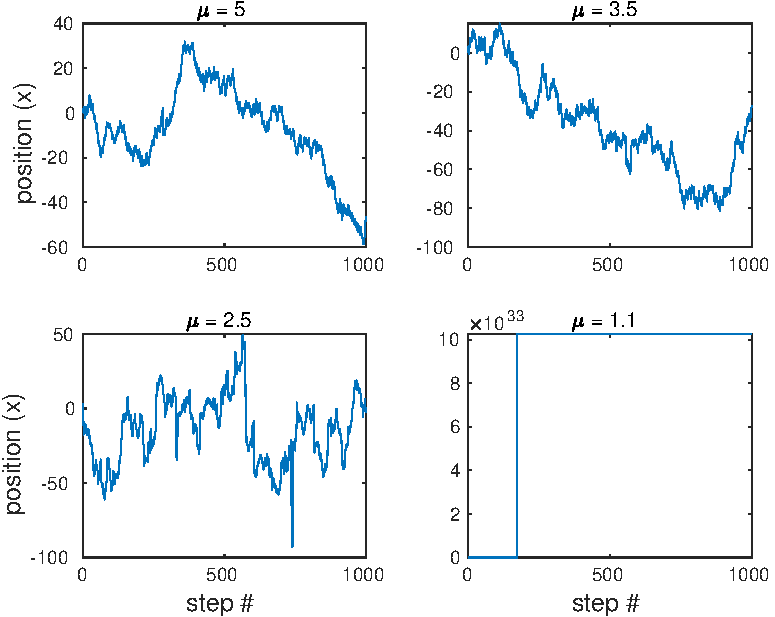
\includegraphics[width=0.8\textwidth]{RandomWalk-PowerLaw}
		\caption[Comparison of different choices of parameter for a random walk with power-law distributed steps]{A realisation of a random walk with power-law step-length distribution, simulated over $1000$ time steps for $x_{\min}=1$ and four different choices of parameter $\mu$. The top-left ($\mu=5$) and top-right ($\mu=3.5$) plots correspond to Brownian motion in the scaling-limit, and the bottom-left ($\mu=2.5$) and bottom-right ($\mu=1.1$) are L\'{e}vy flights.}
		\label{fig:RandomWalk-PowerLaw}
	\end{figure}

\end{subsection}


\end{section}
\FloatBarrier
%\input{chapter-background/technicalterms}
%!TEX root = ../thesis.tex

\begin{section}{Literature Review \label{sec:litreview}}


\iffalse The search for food is one of the most important factors when investigating animal behaviour, and when considering where an animal travels, it is often the most important factor \cite{}. Animal foraging patterns are often not just patterns of how an animal searches for food, but actually provide insight into an animal's overall movement pattern. The study of how effective an animal's foraging strategy is can act as a very good proxy as to how likely an animal is to survive \cite{}. 

It is this reasoning with which the field of Optimal Foraging Theory hypothesises that animal's should have evolved to use a foraging strategy that is highly optimised. We make it clear that we expect highly optimised models to arise, rather than the most optimal strategy itself, since animal foraging strategies are not indicative of reproduction rate, but rather, the survival rate - and are only a proxy at that.

\fi
James \etal \cite{James_2011} gave a thorough overview of stochastic optimal foraging theory in 2011, and discussed both the latest results as well as the history of the field.
Our literature review follows a similar structure to their paper, by first examining in detail a few of the early papers in the field, before discussing various extensions that have been made to the basic model.
Since this thesis does not investigate any actual movement data, but rather focusses on the theoretical side of the problem, we emphasise the findings and methods of papers that focus on theoretical models. Furthermore, we place the heaviest emphasis on papers that consider various regime-switching strategies or where model parameters such as the radius of vision may vary.

\subsection{Early evidence for L\'{e}vy flight foraging strategies}

\subsubsection{Empirical evidence in favour of L\'{e}vy flights}

The earliest evidence of L\'{e}vy flights in foraging data came in the form of scale-invariance in the activity periods of Drosophila, a genus of fruitfly.
Cole \cite{Cole_1995} examined the activity periods of said Drosophila, and observed that they appeared to be undergoing activity constantly.
Upon magnification, this constant activity turned out to be multiple bouts of activity, with short bouts of inactivity between.
Further magnification revealed that these smaller bouts of activity were once again made up of even smaller episodes of activity with inactivity between these, suggesting a self-similar structure.
By plotting on a log-log plot the total number of intervals of inactivity as a function of the length of time required to consider a period inactive, a slope of $-1.37 \pm 0.12$ was found, and thus it was concluded that the temporal distribution of the activity of fruitflies has a fractal structure.
The slope being less than $-1$ implied that the larger the threshold of time that is used to discern between activity and inactivity is, the total amount of time spent inactive increases.
Finally, Cole concluded that if we assumed the flies moved at a constant rate during active phases, then the fractal switching of movement activity would translate into fractal space use, producing a L\'{e}vy flight. 

Viswanathan \etal \cite{Viswanathan_1996} investigated the presence of long-range correlations in the movement data of wandering albatrosses by considering a random walk, $Y(t)$, to represent the net displacement of an albatross.
The \emph{mean square displacement} of the albatross is given by 
\[F(t) = \sqrt{ \E{ \Delta Y(t))^2 } - \E{ \Delta Y(t) }^2}, \]
where $\Delta Y(t) := Y(t_0+t) - Y(t_0)$.

An uncorrelated random walk, or a Markov process for a sufficiently large $t$, would result in
\[F(t) \sim t^\alpha, \]
with $\alpha = 1/2$, due to the Central Limit Theorem \cite{Viswanathan_1996}.
The mean square displacement, when plotted on a log-log plot against time, demonstrated a power law relationship with $\alpha = 0.84 \pm 0.2 \neq 1/2$, implying that long-range correlations do, in fact, exist in the wandering albatross data.
By plotting the sum of the power spectra against the time period used on a linear plot, and against the frequency on a log-log plot, they were able to further confirm the existence of long-range correlations as well as scale invariance.
To determine the origin of the scale invariance, the authors plotted the distribution of flight-time intervals on a log-log plot, and found that the data approximately fitted a power-law distribution, with a slope of $\mu \approx 2$. 

The authors also used numerical simulations to determine the mean square displacement fluctuations that would be observed under a L\'{e}vy flight model in which the probability density for a flight time, $t$, is given by
\[p(t) \sim (t + 1)^{-\mu} ,\]
where the `$+1$' is introduced to account for the bird spending exactly one unit of time each time it lands.
Fixing $\mu = 2$ in this model, based on the observed slope from the flight-time data of wandering albatrosses, the mean square displacement was found via numerical simulations.
The simulation of this model yielded long-range correlations with $\alpha = 0.8 \pm 0.05$, which was consistent with the long-range correlation found from the data. 

The reasons for the landing points of wandering albatrosses being spatially scale-invariant was speculated on by Viswanathan \etal \cite{Viswanathan_1996}, with one possible reason being that the distribution of food is also scale invariant.
Another possible explanation is related to the lifetime distribution of the thermal columns that birds use to produce lift.
A potential advantage may also be found by considering foragers that operate as a flock, rather than an individual.
An individual L\'{e}vy walker visits $t$ new sites in the time that an individual Brownian walker visits $t/\ln t$ sites, whereas a flock or swarm comprised of $N$ L\'{e}vy walkers finds $Nt$ sites, while a swarm of Brownian walkers visit $t \ln(N/\ln t)$, making the improved efficiency of the L\'{e}vy flight pattern considerable when dealing with large flocks.
Since evidence of L\'{e}vy flights was found for albatrosses, the authors suggest further work should be done examining other animals for L\'{e}vy flight patterns.

Using the same methods as previous papers \cite{Cole_1995,Viswanathan_1996}, Viswanathan \etal \cite{Viswanathan_1999} investigated the foraging behaviour of bees, wandering albatrosses, both fenced and unfenced deer, and amoeba.  Using log-log plots and line of best fit, the flight-length distribution was found to fit a power-law distribution with $\mu \approx 2$, which matched the theoretical optimal strategy that they found.
The amoeba data was found to fit a power-law with $2 \leq \mu \leq 2.5$, which also corresponds to a L\'{e}vy walk.

Recent reanalysis of the empirical evidence has contradicted some of these conclusion. In particular, Edwards \etal \cite{Edwards_2011} devised a \ac{MLE} method to determine more rigorously whether movement data fits a particular distribution. Using this, they revisited many of the original animals that were investigated using higher resolution datasets and found that most did not undergo L\'{e}vy flights. Towards the end of the literature review we discuss the more recent statistical methods, the reanalyses of the empirical results, and some further problems with data analysis in the field of animal foraging, in further detail.

\subsubsection{Basic theoretical models for animal foraging}

Following the empirical evidence of L\'{e}vy flights, Viswanathan \etal \cite{Viswanathan_1999} investigated what search strategy provides a theoretical optimal for a simplified model.
Their model was two-dimensional and they looked at both \emph{destructive} and \emph{non-destructive foraging}.
The \emph{search efficiency} was defined to be
\begin{equation*}
\eta = \frac{1}{\E{\ell}N},
\end{equation*}
where $\E{\ell}$ is the mean flight distance, and $N$ is the mean number of steps taken to find food.
The step lengths taken by foragers were drawn from a power-law distribution.
By assuming the \emph{mean free path} between successive targets, which we denote as $\lambda$, are all equal, and denoting the forager's \emph{radius of vision} as $r_v$, the mean flight distance was expressed as 
\begin{equation*}
\E{\ell} = \frac{\int_{r_v}^{\lambda}\ell^{1-\mu}d\ell+ \lambda \int_{\lambda}^{\infty}\ell^{-\mu}d\ell}{\int_{r_v}^\infty \ell^{-\mu}d\ell},
\end{equation*}
which can be solved exactly.
The mean number of steps taken to find a target is denoted either $N_d$ or $N_n$, for destructive and non-destructive foraging, respectively. 

To solve for $N_d$, the authors defined $\mu-1$ as the fractal dimension of the sites, and then used an existing result \cite{Geisel_1985} to determine that the mean number of steps until a target is found to scale as $N_d \approx (\lambda/r_v)^{\mu-1}$, for $1 \leq \mu \leq 3$, which is valid for the destructive case.
If $\mu \geq 3$, which corresponds to Brownian motion, then the mean steps scale as $N_d \approx (\lambda/r_v)^2$.
To solve for non-destructive foraging, they showed that $N_n \approx N_d^{1/2}$ using a one-dimensional Brownian walker.
More specifically, a Brownian walker at the middle of an interval has $N_d = \lambda^2/(2D)$, where $D$ is the diffusion constant, and a Brownian walker at some small distance, $r_0$, from the edge of an interval has $N_n= (\lambda-r_0)r_0/(2D)$.
This implies that $N_n \approx N_d^{1/2}$, and the authors assumed that this relation remains true even for $\mu < 3$, and thus arrived at $N_n \approx (\lambda/r_v)^{(\mu-1)/2}$ for $1 \leq \mu \leq 3$.

Then, with their approximate expressions for the efficiency, Viswanathan \etal \cite{Viswanathan_1999} determined the most efficient strategy for a range of different scenarios.
When target sites are plentiful, $\lambda \leq r_v$ and so $N_d \approx N_{n} \approx 1$, meaning the efficiency is independent of search strategy.
For sparse targets, the efficiency for destructive foraging was found to asymptotically increase as $\mu \to 1$, corresponding to ballistic motion.
For non-destructive foraging when targets are sparse, an optimum was shown to exist at $\mu = 2 - \delta$, where $\delta \approx [\ln(\lambda/r_v)]^{-2}$, which corresponds to a L\'{e}vy flight.

Viswanathan \etal \cite{Viswanathan_1999} verified the validity of their conclusions by performing numerical simulations, which were found to match the analytic approximations they had derived.
Further, the fact that the optimal strategy for non-destructive foraging matched previous empirical results \cite{Cole_1995,Viswanathan_1996} strengthened the validity of the model.
Thus, their model seemed to be simple enough to obtain some analytic results, while still being complex enough to consider various different scenarios and maintain realism.
This paper became one of the foundations of stochastic animal foraging theory, with many papers building upon this model.

Bartumeus \etal \cite{Bartumeus_2013} considered a one-dimensional foraging model, which they showed can be reduced to a single interval with absorbing boundaries at either end representing food targets. They considered a forager doing a random walk with an arbitrary step-length distribution, and found an exact expression for the expected total length until food is found, and hence the foraging efficiency. Some of the results of this paper already existed \cite{Buldyrev_2001_avetime,Buldyrev_2001_prop}, although not in the context of animal foraging. They confirmed the optimal efficiency of a power-law random walk occurs at $\mu=2$, representing a L\'{e}vy walk.

\subsubsection{Further empirical investigation and methodology}

The evidence of L\'{e}vy flights in animal foraging data \cite{Cole_1995,Viswanathan_1996,Viswanathan_1999} sparked an interest in investigating the step-length distribution of many different species of animals, with many papers following these first three.
Most species investigated were found to have some evidence of L\'{e}vy flight movement paths (e.g. \cite{Marell_2002,Ayala_Orozco_2004,Reynolds_2007_moths,Reynolds_2007_bees,Sims_2008}), although this was not the case for every species (e.g. \cite{Austin_2004}). 

Much of the investigation of animal movement data used the same methods as the original L\'{e}vy flight papers of Cole \cite{Cole_1995}, and Viswanathan \etal \cite{Viswanathan_1996}.
The most commonly used technique was plotting the distribution of step-lengths on a log-log plot to determine the parameter of the power-law distribution.
Mårell \etal \cite{Marell_2002} investigated semidomesticated female reindeer, for which the line of best fit on a log-log plot of the step-length distribution had a slope of $\mu=1.8$ or $\mu=2$ depending on the time-scale.
Ayala-Orozco \etal \cite{Ayala_Orozco_2004} studied the movement patterns of free-ranging spider monkeys and found that the fitted power-law distribution has parameter $\mu=2.18$.
Austin \etal \cite{Austin_2004} found that only 15.3\% of grey seals had movement data that fit a negative power law distribution based upon regression lines on a log-log plot, and suggested that the lack of evidence for L\'{e}vy flight may be indicative of non-randomly distributed food items.
Sims \etal \cite{Sims_2008} used a log-log plot to determine the power-law parameters for penguins ($\mu=1.7$, $r^2 = 0.91$), sharks ($\mu=2.4$, $r^2=0.90$), as well as sea turtles and various bony fish, which had parameters between that of penguins and sharks.
Reynolds \etal \cite{Reynolds_2009_fractional} investigated Drosophila again, and found that a power-law distribution with a parameter of $\mu \approx 2$ provided the best fit.
Reynolds \etal \cite{Reynolds_2007_moths} found the frequency distribution of the appetitive Agrotis segetum moths to fit a power-law distribution with $\mu=1.5$.
This value of $\mu$ is consistent with the optimal parameter for a biased L\'{e}vy flight, which has $1 < \mu \leq 2$.
Reynolds \etal \cite{Reynolds_2007_moths} reasoned that a biased strategy occurred due to the way the experiment was conducted, with the detection of pheromones depending on whether or not the target was upwind or downwind.

Some other methods were also used in investigating animal movement data.
Reynolds \etal \cite{Reynolds_2007_bees} considered the mean square displacement of the flight lengths of honey bees, $F(t)$,  finding $F(t) \propto t^\alpha$, where $\alpha=0.85 \neq 0.5$, which is indicative of long-term power-law correlation.
This scale-free behaviour is consistent with a L\'{e}vy walk with $\mu \approx 2$, and the scaling exponent found can be reproduced with a truncated L\'{e}vy flight with $\mu = 2$.
Sims \etal \cite{Sims_2008} also plotted the mean square displacement of the displacement of various sea creatures, and found values of $\alpha$ between $0.80$ and $1.24$, which implies a long-term correlation and indicates scale-invariance in the movement pattern.
Ayala-Orozco \etal \cite{Ayala_Orozco_2004} also considered an exponential distribution ($r^2=0.79$) for the step-length distribution, although the power-law ($r^2=0.89$) was shown to provide a better fit.
Mårell \etal \cite{Marell_2002} found the fractal dimension in reindeer movement lengths to be between $1.0$ and $1.5$, with the time-scale having no effect.
The fractal dimension of Brownian motion is $2$, and thus they concluded that Brownian motion was not a good fit for reindeer movement, which implies that a L\'{e}vy flight may be a better fit.

Evidence was also found for heavy-tailed distributions in various other aspects of animal movement, beyond just the distribution of step-lengths.
Ayala-Orozco \etal \cite{Ayala_Orozco_2004} found evidence of a heavy-tailed distribution of waiting times in the movement of spider monkeys, with a power-law distribution ($\mu = 1.7$, $r^2 = 0.86$) providing the best fit.
Sims \etal \cite{Sims_2008} examined horizontal krill density in the current of a water column passing an echosounder.
The frequency distribution of changes in krill density was plotted on a log-log plot, and found to fit a power-law distribution with $\mu=1.7$.
Since krill is consumed by some of the predators from the study, this finding suggested that the existence of L\'{e}vy flight behaviour in predator movement may be in response to prey distribution. 

Sims \etal \cite{Sims_2008} suggested two possible explanations for the existence of L\'{e}vy flight behaviour in animal foraging movement: animal search patterns are adapted to stochastically optimise their search for food and are essentially `blind' at the spatio-temporal scale that they search at, or search patterns that are apparently optimal simply arise as a function of the distribution of the prey.
The authors provided further support for the latter explanation, by showing that L\'{e}vy walk search strategies have advantages in landscapes with fractal prey distributions compared to other prey distributions.
Through numerical simulations of vertical diving movement, the encounter rate of both L\'{e}vy walks and random searches in both L\'{e}vy and fractal prey fields are tested, finding that L\'{e}vy walks in L\'{e}vy environments had encounter rates 14\% higher than in random environments.

\subsection{Extensions to the basic foraging model}

\subsubsection{Foraging for moving targets}

Bartumeus \etal \cite{Bartumeus_2002} considered the case of foraging for moving targets, which can be thought of as a \emph{predator} searching for moving \emph{prey}.
The authors performed a simulation study of a single forager and a single moving target in one-dimension on an interval of length $L$, with periodic boundary conditions, this domain is equivalent to a circle with perimeter $L$.
Varying the size of the system, $L$, effectively varies the density of food targets.
Both the searcher and the target move with a constant velocity, and each step $j$ that they take is in a random direction and of length $\ell_j$, where $\ell_j$ is chosen from a power-law distribution.
Efficiency was defined to be the encounter rate per unit distance travelled by the searcher.
The ratio of \emph{searcher velocity} to \emph{target velocity} was denoted $v$, and the ratio of size --- usually representing either physical size or detection radius --- between the searcher and the target was $r$.
Both the target and the searcher adopt either Brownian ($\mu=3$) or L\'{e}vy ($\mu=2$) searches.
The simulation was repeated, and after an encounter the target is destroyed and a new one created in a random location.
As the system size gets larger, the relative efficiency of a L\'{e}vy walk search compared to a Brownian search increases.
When the targets move according to a Brownian motion, a L\'{e}vy walk search is the most efficient, except for the extreme case of very large (approximately $r\geq 10$) and fast moving targets (approximately $v \geq 10$).
However, when the food targets follow a L\'{e}vy walk, a Brownian search often outperforms a L\'{e}vy search; for example, when target density is high ($L = 25$), Brownian search outperforms L\'{e}vy search when $r>1$ and $v>1$.
The authors found that with Brownian targets, size ratio and velocity ratio are both equally important, but with L\'{e}vy targets, velocity ratio is more important than size ratio.

James \etal \cite{James_2008} continued investigating this same model of moving searcher and target, and confirmed the results that a L\'{e}vy search outperforms a Brownian search for Brownian targets, with its relative advantage greater when $v$ is smaller.
However, the authors did not restrict themselves to just $\mu=3$ and $\mu=2$ for the searcher as Bartumeus \etal \cite{Bartumeus_2002} did, but instead investigated an entire spectrum of values from $\mu=1$ to $\mu=3$, with the food target following either a ballistic path ($\mu\to 1$), L\'{e}vy walk ($\mu=2$), or Brownian motion ($\mu=3$).
They found that a ballistic search actually outperforms both a L\'{e}vy search and a Brownian search in all but one case --- the unrealistic case when the searcher and target have identical speeds ($v=1$) and travel in the same direction, never encountering one another.
The authors also derived an analytic expression for the mean efficiency of a ballistic search, $\eta$, based on a geometric approach
\begin{equation*}
\eta = \begin{cases}
2(1-v^2)/L \quad \text{for } v \leq 1,\\
[2(v^2 - 1)]/(Lv) \quad \text{for }v \geq 1.
\end{cases}
\end{equation*}
James \etal \cite{James_2008} also extended the model by considering many moving targets, each moving independently of each other, which they argued is a more accurate approximation of a higher-dimensional setting.
They assumed the searcher begins at $0$, and considered the case of evenly-spaced targets at $(2n-1)L/2$, $n\in \mathbb{Z}$, as well as the case with uniformly distributed targets, both cases having the same target density.
A predator using a ballistic search was once again shown to be more efficient than either a Brownian or L\'{e}vy search.

Faustino \etal \cite{Faustino_2007} considered the same model as James \etal \cite{James_2008}, although only the case of $v=1$, and rather than using a pure power-law distribution, they instead used a truncated power-law distribution.
The optimal search strategy was found to be when $\mu=1$, which does not break down in this case as it did in James \etal \cite{James_2008}, since it is not actually ballistic motion.
James \etal \cite{James_2008} declared that the efficiency of this truncated power-law search with $\mu=1$ is the same as the ballistic search when $v \geq 1$, and is outperformed by the ballistic search when $v<1$.
James \etal \cite{James_2008} concluded that the superior efficiency of the ballistic search against all others, and of the L\'{e}vy search over the Brownian search, is due to the lack of backtracking allowing more ground to be covered by the searcher.
James \etal \cite{James_2008} also pointed out that the work of Bartumeus \etal \cite{Bartumeus_2002} is somewhat flawed: it considered only the size ratio $r_t/r_p$ and not the absolute values, although the sum of their sizes, $r_t + r_p$, relative to the system size, $L$, is actually what determines the target density. Keeping $r_t+r_p$ fixed and varying the ratio $r_t/r_p$, Faustino \etal \cite{Faustino_2007} showed that the efficiency does not change.

Bartumeus \etal \cite{Bartumeus_2008_super} performed another simulation study, this time considering a range of $\mu$ between $1$ and $3$, as well as varying target density, target size, target cruising velocity, and both destructive and non-destructive searches, on $1$D, $2$D, and $3$D search spaces.
Their results confirmed the results of James \etal \cite{James_2008} for the destructive case, and found that $\mu \approx 2$ is most efficient for the non-destructive case, with the exact value depending on the system's parameters.
They noted that although increasing the dimension reduces the relative efficiency of one strategy over another, it does not change what the optimal strategy is.
When targets travel slower than the searcher, the encounter rates are affected only by the search strategy of the searcher, and when searchers travel slower, the encounter rates are affected only by the movement strategy of the target.
That is, the encounter rate depended only on the movement strategy of the faster moving organism.
When both searcher and target move at similar speeds, the most efficient search strategy for the searcher was to use a L\'{e}vy search with parameter as far away from the parameter of the targets L\'{e}vy movement as possible (e.g. $\mu=3$ if the target is moving according to $\mu \to 1$, and $\mu \to 1$ if the target is moving according to $\mu=3$).

\subsubsection{Food targets with a revisitability delay}

Raposo \etal \cite{Raposo_2003} studied the role of a \emph{delay time} --- or \emph{revisitability delay} --- which was denoted $\tau$.
After an animal finds a food target, the same target cannot be revisited until $\tau$ time has elapsed since originally visiting it.
A revisitability delay essentially provides a continuum between non-destructive ($\tau = 0$) and destructive foraging ($\tau = \infty$).
Raposo \etal began with the model outlined by Viswanathan \etal \cite{Viswanathan_1999} and extended it by adding a delay time to the targets.
To determine the optimal strategy, the authors used a result from the one-dimensional case found by Buldyrev \etal \cite{Buldyrev_2001_prop}, that if a forager begins at a point $x=z\lambda$ in the interval $[0,\lambda]$ with $0<z<1$ and $\lambda/\lmin \to \infty$, the optimal parameter for a power-law strategy is
\begin{equation*}
\mu_{\text{opt}} = 2 + \frac{2}{\log z} + o\left(\frac{1}{\log z}\right).
\end{equation*}
Raposo \etal \cite{Raposo_2003} related the distance $z\lambda$ to the forager's velocity and the delay time by
\begin{equation*}
z = \frac{v \tau}{\lambda}.
\end{equation*}
This is based on the assumption that the forager moves at a constant velocity $v$ away from the target during the delay time, and then begins its search again once the delay time expires, which will be at point $z \lambda$.
Using this, the authors showed that the case of $\tau \to 0$ implies that $z \to 0$ and $\log z \to -\infty$ and hence $\mu_{\text{opt}} = 2$.
Similarly, when $z > 1/e^2$ --- which occurs when $\tau > \lambda/(v e^2)$ --- the optimal strategy is $\mu < 1$, corresponding to straight line motion with constant velocity.
Although the optimal efficiency is not known exactly for higher dimensions, Raposo \etal \cite{Raposo_2003} argued that the results of the one-dimensional case have validity since in $d$ dimensions the forager moves through a one-dimensional corridor of cross section proportional to $r_v^{d-1}$, and they confirmed this for the two-dimensional case using simulations.
The authors concluded that the most efficient strategy is strongly dependent on the delay time of the targets as long as $\lmin \geq r_v$, where the efficiency is defined as the number of targets found per distance travelled, with $1 < \mu_{\text{opt}}(\tau) \leq 2$, based on the two limiting cases of destructive and non-destructive foraging. 
	
Raposo \etal \cite{Raposo_2003} also considered a more general cost function, $f(\E{L})$, which is a function of the expected distance to find a single target.
This definition of efficiency can take into account various phenomena that make the model more realistic, such as energy gain due to calories and nutrients in the targets.
The optimal values of $\mu$ for a L\'{e}vy walk do not change when using this more general notion of efficiency, although depending on the cost function the values that $\mu$ can take may be limited. 

Santos \etal \cite{Santos_2004} further investigated a delay time, and extended the results of Raposo \etal \cite{Raposo_2003} by effectively interpolating between the two known results, which are the limiting cases of destructive ($\tau \to \infty$) and non-destructive foraging ($\tau = 0$).
As found originally by Viswanathan \etal \cite{Viswanathan_1999}, the expected number of steps to find a food target scales as $N_s \sim \lambda^{(\mu -1)/2}$ for a search beginning at $x_0=r_v$ (non-destructive), and $N_s \sim \lambda^{\mu-1}$ for $x_0=\lambda/2$ (destructive).
Based on this, Santos \etal \cite{Santos_2004} determined the more general form for the mean number of flights,
\begin{equation*}
N_s \sim \lambda^{(\mu-1)/\Gamma},
\end{equation*}
where $\Gamma=2$ and $\Gamma=1$ are the two limiting cases for non-destructive and destructive foraging, respectively.
The authors then considered $\Gamma(\tau)$, as a monotonically decreasing function with $\Gamma \to 2$ when $\tau \to 0$ and $\Gamma \to 1$ when $\tau \to \infty$.
Using this function, Santos \etal \cite{Santos_2004} arrived at an expression for the efficiency depending only on the value of $\Gamma$ as well as the ratio $\lambda /r_v$.
The authors then plotted the efficiency of a L\'{e}vy search for a range of different values of $\tau$, showing the crossover between the two different limiting cases.
Santos \etal \cite{Santos_2004} also considered the effect of a more general cost function which takes into account the forager's energy, and concluded that optimal parameters will not be affected by this different notion of efficiency, matching the conclusions of Raposo \etal \cite{Raposo_2003}.

\subsubsection{Two-dimensional and three-dimensional foraging}

Santos \etal \cite{Santos_2005} considered a two-dimensional search on a lattice, with two different types of lattice topology: a \emph{square lattice}, with $4$ possible directions from each node, and a \emph{triangular lattice}, with $6$ possible directions from each node.
Targets were assumed to be distributed homogeneously among the nodes of the lattice, and both the non-destructive and destructive cases were considered.
A forager would choose a uniformly random direction and a step-length from a power-law distribution.
If a target is within a distance $r_v$ of a forager, the forager may move directly to it if there is a straight-line path towards it, meaning zigzag paths were restricted.
Using this simplified model, the authors were able to obtain some analytic results.
A L\'{e}vy walk with $\mu \approx 2$ was only optimal for low target densities, with a ballistic path being the optimal strategy for higher target densities.

Santos \etal \cite{Santos_2008} \etal built upon the previous two-dimensional lattice model \cite{Santos_2005}, by introducing \emph{defects} that were randomly scattered throughout the lattice.
Under their model, foragers would travel in a straight line until they came into contact with a defect, after which they would choose a new direction and distance. One way of thinking about defects is as food patches that are found to be empty upon arriving at them.
The optimal strategy was found to heavily depend on the density of targets and defects, as well as the boundary conditions employed.
For $\mu >2$, the average step length is small and so truncation does not happen very often; consequently, the density of food patches and defects matter somewhat less, and the boundary conditions have almost no effect on the optimal strategy.
Raposo \etal \cite{Raposo_2009} also considered a very similar model to Santos \etal \cite{Santos_2008}, involving a lattice with defects.
Using both analytic approximations and simulations they came to similar conclusions as Santos \etal \cite{Santos_2008}, finding that as the presence of defects increases, the relative advantage of one strategy over any other decreases.

\subsection{Composite search strategies for improved efficiency}

\subsubsection{Foraging strategies with a giving-up time}

Benhamou \cite{Benhamou_2007} considered \emph{composite Brownian walk} strategies as alternatives to L\'{e}vy walk strategies when searching in a \emph{patchy environment}. 
A composite Brownian walk is a mixture of two random walks, both with exponentially-distributed step sizes. 
A patchy environment was here defined to have uniformly distributed patches of food, and within these patches the density of food is much higher than the density of food outside of the patches.
The forager considered by Benhamou began with an extensive search, in which large steps were drawn from an exponential distribution, and switched to the intensive search once a food patch was reached, with step-lengths also drawn from an exponential distribution, with different parameters resulting in a smaller mean.
After some time, referred to as the giving-up time, had elapsed, the forager would switch back into the extensive movement mode.
In a patchy food environment with destructive targets, the forager begins its next search in the vicinity of a target since multiple targets are clumped together, and so this scenario is equivalent to the non-destructive scenario of Viswanathan \etal \cite{Viswanathan_1999}.
Through simulations, Benhamou \cite{Benhamou_2007} showed that a composite Brownian walk appeared to be more efficient than a L\'{e}vy walk for finding food in a patchy environment.

Plank and James \cite{Plank_2008} derived some analytic results for a similar model in one dimension, in which a forager follows a Brownian motion for its intensive search, before giving-up and undergoing ballistic motion for its extensive search.
They reasoned that, due to the Central Limit Theorem, the discrete model of Benhamou \cite{Benhamou_2007} will converge to their model after a large number of steps, as long as the variance of the step-length distribution is finite.
In deriving an expression for the density of the total distance travelled to find food, they used an existing result for the density of Brownian motion with an absorbing barrier at $x=0$, from Grimmett and Stirzaker \cite{Grimmett_2001}. 
This also means that the results are only valid for strategies which have Brownian motion as the intensive search strategy, but not a L\'{e}vy walk, for example.
With their model, Plank and James \cite{Plank_2008} derived an analytic expression for the optimal giving-up time, as well as showed that the composite Brownian walk strategy outperforms a L\'{e}vy walk strategy, in agreement with the results of Benhamou \cite{Benhamou_2007}.

\subsubsection{Adaptive L\'{e}vy walks as a more general giving-up time strategy}

Reynolds \cite{Reynolds_2008_comment} explained that the composite Brownian walk search of Benhamou \cite{Benhamou_2007} can actually be viewed as a special case of an \emph{adaptive L\'{e}vy walk search}. 
An adaptive L\'{e}vy walk involves switching between a L\'{e}vy walk with $\mu \to 1$ for the extensive search, and a L\'{e}vy walk with $\mu=3$ for the intensive search.
Then, Reynolds argued, that when considering the CBW as an adaptive L\'{e}vy walk the results of Benhamou \cite{Benhamou_2007} follow directly from the L\'{e}vy walk search theory of Viswanathan \etal \cite{Viswanathan_1999}, since a L\'{e}vy walk with $\mu \to 1$ was optimal for sparse targets, and $\mu=3$ for densely distributed targets.
Benhamou \cite{Benhamou_2008} replied to Reynolds \cite{Reynolds_2008_comment}, pointing out that the composite Brownian walk could not be thought of as an adaptive L\'{e}vy flight for two reasons: the inverse power-law has infinite variance when $1 < \mu < 3$ and so $\mu =3$ does not correspond to a L\'{e}vy flight, and when $\mu \to 1$ a L\'{e}vy flight tends to a straight line of infinite length and so must be truncated, effectively making the variance finite. 
Benhamou's criticism is mostly valid, since to be Brownian motion (in the scaling limit), a strategy must have a step-length distribution with finite variance, whereas a L\'{e}vy walk uses a power-law distribution with infinite variance, by definition.
However, this disagreement between Reynolds and Benhamou is ultimately over little more than semantics, since if although a power-law with $\mu =3$ is technically not a L\'{e}vy walk, there is no mathematical reason as to why the step-length distribution cannot have $\mu=3$. For example, if the adaptive L\'{e}vy walk search model was instead referred to as an adaptive power-law search model, since the power-law can produce both a L\'{e}vy walk and a Brownian motion, then the conclusions of Reynolds \cite{Reynolds_2008_comment} would still be true.

Reynolds \cite{Reynolds_2009_adaptive} then considered the adaptive L\'{e}vy walk model but allowed for any value of $\mu$ during the extensive phase, which reduces to the CBW model of Benhamou \cite{Benhamou_2007} when $\mu \to 1$.
This time it was used to investigate non-destructive foraging ($x_0=r_v$), which as previously shown \cite{Reynolds_2008_comment} is equivalent to foraging in a patchy environment.
It was determined that the optimal extensive parameter was between $\mu=1$ and $\mu=2$, with a higher food target density moving the optimal closer to $\mu=2$.
James \etal \cite{James_2011} noted that Reynolds \cite{Reynolds_2009_adaptive} only considered a fixed giving-up time, whereas Plank and James \cite{Plank_2008} optimised over all giving-up times.

Nolting \cite{Nolting_2013} investigated composite strategies such as giving-up time strategies, as well as a new type of strategy that a forager may use, which they called the \emph{optimal zone forager}.
As with the giving-up time strategy, the optimal zone forager switches between an intensive and extensive search, although this time depending on its current location.
Thus, the forager must have \emph{a priori} knowledge of where the food targets are located, although it cannot use this knowledge to move directly to a resource, but rather it can only change modes.
For a strategy that uses a Brownian motion and ballistic motion for its intensive and extensive search, Nolting reasoned that the optimal zone forager is ideal.

\subsubsection{Searching for difficult-to-detect targets}

A one-dimensional composite model was also considered by Bénichou \etal \cite{Benichou_2005}, in which a forager switches between an intensive phase, also known as the \emph{searching phase}, and \emph{extensive phase}, also known as the \emph{relocation phase}.
In this model, the forager was incapable of detecting targets during the relocation phase, and so the model was referred to as searching for hidden targets. 
The time spent in each phase was exponentially distributed, and the forager could switch back-and-forth between phases an unlimited number of times.
As with many of the other composite strategies (e.g. \cite{Plank_2008,Benhamou_2007}), the intensive phase consists of Brownian motion, and the extensive phase is ballistic motion which is always in the same direction.
This persistence in the direction of the extensive search was referred to as \emph{orientational memory}, and was also addressed by later papers.
A uniform density of patches is assumed, and so the problem is reduced to finding patches in a single interval, as done in other papers (e.g. \cite{Bartumeus_2013}).
The authors considered a forager that begins at the middle of an interval, which corresponds to destructive foraging.
Using an analytic argument, they found that the optimal search strategy under their model occurs when the average duration of the searching phase, denoted $f_1$, is proportional to the average duration in the relocation phase, denoted $f_2$, by either $f_1 \propto f_2^{3/5}$ or $f_1 \propto f_2^{2/3}$ depending on the frequency of the switching.

Bénichou \etal \cite{Benichou_2006_intermittent} considered the effect of how difficult a target is to detect, and whether this changed the optimal search strategy.
Two types of targets were considered, those that are easy to detect, and those that are difficult to detect, referred to as \emph{hidden}.
A difficult to detect target requires a forager to pass through the area multiple times before it is finally located, whereas an easily detectable target emits a strong enough stimulus to allow a forager walking past to detect it immediately, as long as it is moving slowly enough.
Composite strategies were again considered, with exponentially distributed time between intensive Brownian and extensive ballistic search modes.
For the case of easily detectable targets, it was shown that staying in the active search phase is optimal, as opposed to any composite strategy.
For hidden targets, the optimal strategy was shown to be a composite strategy where the time spent in each phase is as short as possible, which matches the findings of Bénichou \etal \cite{Benichou_2005}.
After removing the forager's orientational memory, the optimal search strategy was found to differ.
With orientational memory, the efficiency scales asymptotically with the mean time spent in each state, whereas without orientational memory the optimal efficiency occurs at finite values for the mean times in each state, which depends on the target density.
The efficiency of searching for hidden targets with orientational memory was found to always be greater than that of searching without orientational memory.

Lomholt \etal \cite{Lomholt_2008} generalised the model of B\'{e}nichou \cite{Benichou_2006_intermittent} by allowing the time spent in the extensive phase to be drawn from either an exponential or L\'{e}vy distribution.
It was found that strategies with L\'{e}vy distributed time spent in the extensive phase outperform the previously investigated strategies with exponentially distributed time in each phase.
Switching between a Brownian motion in the intensive phase and a L\'{e}vy walk in the extensive phase was shown to offer the most efficiency, as well as also being less sensitive to changes in the target density when compared to other strategies.
Of course, these conclusions relied on the forager not being able to detect food during its extensive phase, as discussed by B\'{e}nichou \etal \cite{Benichou_2006_intermittent}.

Bénichou \etal \cite{Benichou_2006} extended the hidden targets destructive foraging model \cite{Benichou_2005} to two dimensions.
They again considered composite strategies, with exponentially distributed time between diffusive searching and ballistic motion.
Taking an approximate analytic approach, they determined that composite two-state strategies optimise the search time required to find a target, as opposed to one-state strategies such as L\'{e}vy flights.

Reynolds \cite{Reynolds_2006} considered the original model of Viswanathan \etal \cite{Viswanathan_1999}, but allowed food to be detected only during a step of length $\ell < \ell_0$, where $\ell_0$ is some fixed threshold.
The optimal parameter for a power-law search was found to be $\mu \approx 2$ for both non-destructive and destructive targets.
If $\ell_0$ is the threshold between a step being considered either intensive or extensive, then Reynolds showed that there is a power-law distributed amount of time spent in each phase.

\subsection{Statistical methods for analysing animal movement data}

As discussed above, many early papers \cite{Cole_1995,Viswanathan_1996,Viswanathan_1999,Marell_2002,Ayala_Orozco_2004,Sims_2008,Reynolds_2009_fractional,Reynolds_2007_moths,Reynolds_2007_bees} found empirical evidence of L\'{e}vy flights in animal movement data.
Most of these \cite{Cole_1995,Viswanathan_1996,Viswanathan_1999,Ayala_Orozco_2004,Sims_2008,Reynolds_2007_drosophila,Reynolds_2007_moths} analysed the movement data by plotting the distribution of step-lengths on a log-log plot, and some \cite{Reynolds_2007_bees,Sims_2008,Ayala_Orozco_2004,Marell_2002} also considered the mean square displacement of the flight lengths.
However, more recent reanalysis has put these methods into question.

\subsubsection{The effect of subsampled data on the apparent step-length distribution}

Benhamou \cite{Benhamou_2007} questioned the validity of using subsampled data to analyse animal movement.
Most animal movement data sets represent a subsample of the animal's movement, since the time between recordings of successive locations is usually significantly longer than time-scale at which an animal moves.
Reynolds \cite{Reynolds_2008_comment} addressed this issue by simulating true L\'{e}vy walk searches with $\mu=2$ and plotting the distribution of subsampled movement lengths, which was still found to fit a log-log plot, though now with $\mu = 1.6$.
Reynolds suggested that subsampling would result in an effective value of $\mu$ less than the true value.

However, Plank and Codling \cite{Plank_2009} found that the sampling rate at which movement data is collected can affect the apparent properties of the movement path, and can even cause misidentification.
Using simulations, they show that it is possible to misidentify a composite correlated random walk which switches between two different phases, as a L\'{e}vy walk, even when using appropriate statistical procedures such as maximum likelihood methods that were previously outlined \cite{Edwards_2007,Plank_2008,Edwards_2008}.
Plank and Codling \cite{Plank_2009} also showed that when a L\'{e}vy walk is subsampled, it can be misidentified as an exponential distribution, with a larger $\mu$ making an apparent exponential more likely.
The point of greatest uncertainty between an exponential and power-law distribution occurs at $\mu \approx 2$.
This conclusion contradicts the claim of Reynolds \cite{Reynolds_2008_comment}, who had not compared the goodness-of-fit with that of another distribution.

To avoid the issues with using data that is a subsample of an animal's true movement path, some papers have instead defined turning points (or reorientation points) which correspond to locations at which a forager changes direction by a significant amount.
Reynolds \cite{ Reynolds_2007_bees} used both \emph{local} and \emph{non-local} determination of a turning point, and found that the statistical properties of the movement distributions do not change significantly between the two.
When determining the turning points \emph{locally}, a new point was said to have occurred when three successive recorded positions of the forager involve a change in direction greater than some critical angle, which in this case was \ang{90}.
\emph{Non-local} determination instead used the cumulative change in angle since the last turning point, with a new point occurring once this was greater than the critical angle.
Since the bee movement distributions found with each of the two methods were not significantly different to each other, this indicated that most direction changes are abrupt, and the authors found that the direction of flight paths are distributed uniformly.
Reynolds \cite{Reynolds_2007_moths, Reynolds_2009_bees} also used local turning point determination when investigating the movement of moths and bees again, and found that the choice of critical angle had no significant effect on the results. 

Codling and Plank \cite{Codling_2010}, however, found that whether or not a movement path is identified as having a power-law distribution depends on both the sampling rate and the designation of turning angles.
They simulate correlated composite random walks and L\'{e}vy walks and find that there is no standard method of turning-point identification that is robust for all cases, with non L\'{e}vy walks often displaying L\'{e}vy-like characteristics.

\subsubsection{Improved identification using MLE methods}

Viswanthan \etal \cite{Viswanathan_2005} proposed a criterion that is necessary, but not sufficient, to establish true superdiffusive behaviour in animal movement data.
If $\tau$ is the estimated correlation time of a general correlated random walk, then the data must display superdiffusive behaviour on scales larger than $\tau$ for there to be true superdiffusive behaviour.

Edwards \etal \cite{Edwards_2007} revisited the movement pattern of albatrosses, now with a higher resolution dataset than the original study \cite{Viswanathan_1996}.
They discussed some of the inadequacies of the usual data analysis methods used throughout the animal foraging literature (e.g \cite{Cole_1995,Viswanathan_1996,Viswanathan_1999,Ayala_Orozco_2004}), and outlined a \ac{MLE} method to determine whether movement data fits a power-law distribution.
They analytically solved the \acp{MLE} for both a power-law distribution and an exponential, and used these to determine the \ac{AIC} and the relative likelihood of each model.
Using their \ac{MLE} method and the new albatross dataset, they determined that there was no evidence of L\'{e}vy flight behaviour in the movement of albatrosses, but rather they followed a gamma distribution.
After correcting the original albatross data \cite{Viswanathan_1996}, they also determined that the original conclusions of L\'{e}vy flights being present in the data were spurious.
Furthermore, they applied their method to the original deer and bumblebee datasets \cite{Viswanathan_1999}, and determined that none exhibited evidence of L\'{e}vy flights.

White \etal \cite{White_2008} compared various methods of fitting data to a distribution, including logarithmic binning and \ac{MLE} methods.
Power-law datasets were generated using Monte Carlo methods, and then using each method the distribution and parameters were determined, before finally comparing the performance of the methods by considering their bias and variance.
Logarithmic binning was found to give an incorrect exponent, and adjustments were necessary to obtain the correct slope.
Further, binning methods in general performed poorly, and White \etal \cite{White_2008} recommended avoiding these whenever possible.
\ac{MLE} methods were shown to be the best approach, and produced valid confidence intervals for the estimated exponents.

\subsubsection{Further issues with identifying L\'{e}vy walks in foraging data}

Plank and James \cite{Plank_2008} simulated a L\'{e}vy walk and a composite random walk and investigated fitting the movement data to step-length distributions.
They determined the best-fit parameters and the log-likelihood for each model, and in both cases found an exponential distribution provided a better fit than the power law distribution.
They conclude that both a L\'{e}vy and a non-L\'{e}vy process can produce a non-L\'{e}vy pattern, which complements the results of Benhamou \cite{Benhamou_2007}, who showed that both a L\'{e}vy and non-L\'{e}vy process can produce a L\'{e}vy pattern.

Following some of the inadequacies found with the early evidence for L\'{e}vy flights in foraging data \cite{Edwards_2007}, Edwards \cite{Edwards_2011} readdressed many of the previous datasets to determine if L\'{e}vy flights really are prevalent in ecology.
He used the modern \ac{MLE} and \ac{AIC} approach \cite{Edwards_2007} to compare L\'{e}vy flights to other simple models, and examined 17 different datasets from previous studies \cite{Austin_2004,Marell_2002,Atkinson_2002,Brown_2006,Bertrand_2007,Marchal_2007,Bartumeus_2003}.
The possible distributions were: unbounded power-law (L\'{e}vy flight), bounded power-law (truncated L\'{e}vy flight), unbounded exponential, and bounded exponential.
Almost all of the original estimates of the parameters were found to lie outside 95\% confidence intervals for the newly calculated parameters.
Further, the evidence of L\'{e}vy flights was overturned for all 17 datasets.
The gray seal dataset was found to have come from a bounded power-law distribution, or a truncated L\'{e}vy flight, and the possibility of the hunter-gatherer dataset coming from a bounded power-law distribution also could not be ruled out.
Three of the 17 datasets were found to fit an unbounded exponential distribution, and the remaining 12 datasets did not match any of the four tested distributions.
Thus, Edwards concluded that L\'{e}vy flight movement patterns are not as common a phenomena in ecology as once thought.

\subsubsection{Empirical evidence for composite strategies}

There has been empirical evidence of animals using composite (or intermittent) strategies, including honeybees \cite{Tyson_2011}, fish \cite{Hills_2002}, birds \cite{Nolet_2002}, turtles \cite{Tyson_2011}, weasels \cite{Haskell_1997}, slime moulds \cite{Latty_2009}, beetles \cite{Ferran_1994}, and others \cite{Benhamou_1994,Reynolds_2009_adaptive,Morales_2004,Klaassen_2006,Jonsen_2007}.

Further, many animals have been found to switch between an intensive and extensive search based on sensory cues from their environment \cite{Sugimoto_1987,Bell_1990,Strand_1982,Persons_1997,Nevitt_2000,Leick_1985,Hellung-Larsen_1990,Dusenbery_1998,Moore_2004,Doving_1994,Dalby-Ball_2000}.
For example, some parasites were shown to use chemical cues to decide when to use an intensive search \cite{Sugimoto_1987,Bell_1990,Strand_1982}, and in a similar way Procellariiform seabirds were shown to use dimethyl sulphide to determine when an intensive search should be used \cite{Nevitt_2000}.

Some of the evidence of composite strategies is based on the qualitative behaviour of animals, while there are also papers that examine the step-length distributions of movement data using various quantitative methods, such as \acp{SSM},\cite{Jonsen_2007}, \acp{HMM} \cite{Joo_2013,Patterson_2017}, Bayesian inference \cite{Parton_2017} and deep-learning models \cite{Browning_2017}.

\iffalse
B\'{e}nichou \etal \cite{Benichou_2011} provided a thorough review of intermittent search strategies, on both the microscopic and macroscopic scale.
They considered intermittent strategies as a slow search phase with possible detection of food, followed by a fast movement phase with no possibility of food detection.
\fi
\end{section}
\end{chapter}


% Chapter 3: One-dimensional models
\begin{chapter}{One-dimensional foraging model\label{sec:1Dmodel}}
%!TEX root = ../thesis.tex
\begin{section}{General assumptions}
\label{sec:1D_introduction}

We consider a forager in one dimension by first defining the search space as the set of all real numbers, $\mathbb{R}$.
That is, the forager can search anywhere along a single dimension.
Targets are equispaced along this search space, a distance of $\lambda$ apart.
\cref{fig:1dmodels:searchspace} shows what this scenario may look like.

\usetikzlibrary{shapes.misc}
\tikzset{cross/.style={cross out, draw=black, minimum size=2*(#1-\pgflinewidth), inner sep=0pt, outer sep=0pt},
	cross/.default={4pt}}
\begin{figure}[H]
	\centering
	\begin{tikzpicture}
	\draw (-5,0) -- (5,0) ; %Draws the big line
	\foreach \x in  {-4,-2,0,2,4}
	\draw[shift={(\x,0)},color=black] node[cross,very thick] {}; %Puts a cross at x = -6,-2,2,6
	\draw[|-latex,very thick] (0,-0.5) -- (2,-0.5) ; %draws the lambda line with left arrow
	\draw[latex-|,very thick] (0,-0.5) -- (2,-0.5) ; %draws the lambda line with right arrow
	\draw (1,-1.2) node[above]{$\lambda$}; %labels the lambda line
	\draw (2,0.2) node[above]{Food target}; %labels the third from left cross.
	\end{tikzpicture}
	\caption[The full search space for the one-dimensional model]{The search space for the one-dimensional foraging model.
	Food patches (crosses) are deterministically spaced along the search space, a distance of $\lambda$ apart.
	\label{fig:1dmodels:searchspace}}
\end{figure}

In reality, food patches will not usually be distributed deterministically and so more realistic one-dimensional models would allow food patches to be distributed along $\mathbb{R}$ according to some probability distribution.
Our assumption of deterministically spaced patches makes solving for the search efficiency easier, and we investigate the effects of making this assumption in \cref{sec:1D_assumptions:deterministic_targets}.

Two types of food patch behaviours are considered: \emph{destructive foraging}, in which the target is destroyed after the forager reaches it, and \emph{non-destructive foraging}, in which the target is not destroyed and can be revisited an unlimited number of times.

Our model assumes that the forager has a radius of vision, $r_v$, with which it can sense any targets that are within $r_v$ of its location.
After a target enters the forager's radius of vision, the forager moves directly to the target.
Initially, we consider a model where the forager has a constant radius of vision, but eventually extend our results in \cref{sec:1dMMRW} to allow the radius of vision to switch based on the state of an underlying Markov chain.

The forager's movement along the $x$-axis is governed by a random process.
In \cref{sec:1dRW}, we consider a strategy in which the forager uses a random walk, with a general step-length distribution.
This is extended to a Markov-modulated random walk strategy in \cref{sec:1dMMRW}.
We are interested only in discrete-time random processes, in which the forager takes discrete ``steps''.
Our notion of a step corresponds to a ``reorientation'' step, in which the animal decides which direction and for what distance it should travel for its next movement, rather than steps representing physical steps made by the forager.
We also disallow the forager from jumping over or skipping targets, and any step that would cause this to occur is truncated.
In one dimension, this assumption is perfectly valid, as there is no way that an animal can pass a target without it at one point being at the target itself.

Our primary aim is to determine the most efficient foraging strategy, where the efficiency is given by
\begin{equation*}
\eta = \frac{1}{\E{L}},
\end{equation*}
where $L$ is the total distance travelled to find the first food patch.
This notion of efficiency is common throughout the literature (e.g \cite{Bartumeus_2013,Viswanathan_1999}) and only considers the distance required to find a single patch.
However, in the case of destructive foraging the food patches are becoming more sparse over time, and so we would expect the efficiency to be decreasing over time.
Because of this, we investigate this notion of efficiency and compare it with others in \cref{sec:1D_assumptions:efficiency}.

Since we are only considering the distance travelled to find a single patch, we can reduce the search space to $[0,\lambda]$, where the two ends of this interval correspond to the targets.
\cref{fig:1dmodels:searchinterval} shows what this new model looks like.
In the reduced model, the assumption of destructive targets corresponds to a search that starts at $\lambda/2$, and that of non-destructive targets corresponds to a search that starts at $r_v$.
This choice of starting locations has been used throughout the literature (e.g. \cite{Bartumeus_2013,}), although we put this on more rigorous grounding in \cref{sec:1D_assumptions:efficiency}.
For now, we provide a brief intuitive explanation of why this is the case.
For a non-destructive forager, after reaching a target and beginning a new search, the target it just found is still available and so its search is beginning right next to a target, at $r_v$.
For a destructive forager, without loss of generality assume that it finds the target at $0$.
Then, for its next search the two nearest patches are at $-\lambda$ and $\lambda$, and its location is halfway between them at $0$.
After scaling this becomes equivalent to starting at $\lambda/2$ on the interval $[0,\lambda]$.

\begin{figure}[H]
	\centering
	\begin{tikzpicture}
		\draw (-1,0) -- (1,0) ; %Draws the big line
		\foreach \x in  {-1,1}
		\draw[shift={(\x,0)},color=black] node[cross,very thick] {}; %Puts a cross
		\draw (-1.0,-1.0) node[above]{$0$}; %labels endpoint
		\draw (1.0,-1.0) node[above]{$\textcolor{black}{\lambda}$}; %labels endpoint
	\end{tikzpicture}
	\caption[The reduced search space for the one-dimensional model]{The search space for a single search, which without loss of generality is the interval $[0,\lambda]$.
	The two food patches are at $x=0$ and $x=\lambda$.
	\label{fig:1dmodels:searchinterval}}
\end{figure}

To determine the efficiency of a search, we shall first derive an expression for $\E{L}$.
Although the overall aim is to determine an expression for the efficiency, we are also interested in determining other quantities for a search, such as the total number of steps taken.
The derivation of many of these quantities is similar in structure, so rather than showing each separately, we first derive the total ``cost'' of a strategy, based on some general cost function for each step.
Using this result, we can determine the efficiency and the total steps taken, among other things, with relative ease.

The derivation of the efficiency of the random walk strategy comes mostly from Bartumeus \etal \cite{Bartumeus_2013}, although some of the results were first found outside of the context of animal foraging \cite{Buldyrev_2001_avetime,Buldyrev_2001_prop}.
The reason for including the derivation in this thesis is twofold.

First, the derivation for the Markov-modulated random walk is fairly similar in structure to that of the random walk strategy.
Some of the techniques that are used require conditions that, while not obvious in the Markov-modulated random walk case, are quite obviously true in the case of the random walk.
Because of this, the paper by Bartumeus \etal \cite{Bartumeus_2013} does not give these details for the random walk strategy.
In particular, applying the Dirac delta function (\cref{thm:1dRW_cost:EV_dirac}) and showing the fact that the operator norm is less than unity (\cref{thm:1dRW_cost:Q_operator_norm}) are not treated by Bartumeus \etal \cite{Bartumeus_2013}.
We include these details that were missed as they help make the derivation for the Markov-modulated case clearer.
Our notation is also reasonably different from Bartumeus \etal \cite{Bartumeus_2013} in order to maintain consistency between the unmodulated and modulated strategies.

Second, the random walk strategy is simple enough to allow us a good insight into why many of the model assumptions are needed, and how relaxing any of these may be difficult.
The notation becomes more complex when Markov-modulation is considered, and much of the intuition is lost.
\end{section}

%!TEX root = ../thesis.tex

\begin{section}{Random walk strategies\label{sec:1dRW}}

The first type of strategy we investigate is the random walk.
Recall from \cref{def:tc:stochastic:randomwalk}, that a random walk is a path of successive steps on some mathematical space.
For the one-dimensional model in question, the mathematical space is the search interval $[0,\lambda]$, although since $r_v$ is constant we may just consider the interval $[r_v,\lambda-r_v]$ as the entire search space.
The forager moves according to a random walk, beginning at some known location $x_0 = a$, for $a \in [r_v,\lambda-r_v]$.

We denote the location of the forager after taking $i$ steps as $X_i$, which is a random variable, or as $x_i$ for a single realisation, for $i \geq 0$.
The length of the $i$th step taken, $\ell_i = X_{i}-X_{i-1}$, is distributed according to some probability distribution, $\ell_i \sim p(\ell)$, which we call the \emph{step-length distribution}.
According to this definition, the length of a step is negative for steps to the left, and positive for steps to the right.
We require $p(\ell)$ to be symmetric about zero, which gives the forager an equal chance of moving in either direction.
The step length is drawn from a distribution with values from $(-\infty,\infty)$, but since the search space is finite, steps moving beyond the boundary will be truncated.
Since a search ends once the forager has left the search interval and hence located food, we are not concerned with where the forager would have ended up after the final step, and instead are concerned with the cost attributed to the final step.
Thus, we avoid having to reconstruct $p(\ell)$ to account for the truncation by instead adjusting the cost function (see \cref{eq:1dRW_cost:cost_truncation}).
We also require that the step-length distribution has a minimum step size, and optionally may have a maximum step size. That is, we consider step-length distributions that have $\abs{\ell} \in [\lmin,\lmax]$, with $\lmin > 0$ since a forager must move every step, and $\lmax \geq \lmin$. For unbounded step-length distributions we have $\lmax \to \infty$.
Once a food patch has been located, the forager stops moving and hence all future positions are the same, given by $X_{\tau} = X_{\tau+1} = \dots$, where $\tau$ is a stopping time corresponding to the time at which the first target is found, and so may take any positive integer value.


\begin{subsection}{Total cost of a random walk strategy\label{sec:1dRW_cost}}

The total cost accumulated to reach a food patch is denoted $Q(x_0)$, where $x_0$ is the starting location of the random walk.
The total cost is, of course, the sum of the cost of every step,
\begin{equation}
	\label{eq:1dRW_cost:Q_sum_q}
	Q(x_0) = \sum_{n=0}^{\tau-1} q(X_n,X_{n+1}),
\end{equation}
where $q(X_n,X_{n+1})$ is non-negative for all $n$.
The cost of a single step, $q(X_n,X_{n+1})$, is a function of the start and end locations of a step, although not of the step number itself.
Recall that we must truncate the cost function for steps that travel beyond the boundaries, and so our cost function becomes
\begin{equation}
\label{eq:1dRW_cost:cost_truncation}
q(X_n,X_{n+1}) = \begin{cases}
q^*(X_n,r_v) \quad &\text{if }X_{n+1} < r_v,\\
q^*(X_n,X_{n+1})  \quad &\text{if } r_v \leq X_{n+1} \leq \lambda-r_v,\\
q^*(X_n,\lambda - r_v) \quad &\text{if }X_{n+1} > \lambda - r_v,
\end{cases}
\end{equation}
where $q^*(X_n,X_{n+1})$ is the function representing the \emph{untruncated} cost of a step from $X_n$ to $X_{n+1}$.

As an example, the untruncated cost function we use when considering the distance travelled on the $n$th step is
\begin{equation*}
q^*(X_n,X_{n+1}) = \left| X_{n+1} - X_n \right|,
\end{equation*}
and hence the cost function will be
\begin{equation*}
q(X_n,X_{n+1}) = \begin{cases}
\left| r_v - X_n \right| \quad &\text{if }X_{n+1} < r_v,\\
\left| X_{n+1} - X_n \right|  \quad &\text{if } r_v \leq X_{n+1} \leq \lambda-r_v,\\
\left| \lambda - r_v - X_n \right|\quad &\text{if }X_{n+1} > \lambda - r_v.
\end{cases}
\end{equation*}

We can rewrite \cref{eq:1dRW_cost:Q_sum_q} to obtain an expression for the total cost where the summation limits do not depend on the random variable $\tau$:
\begin{align}
Q(x_0) &= \sum_{n=0}^{\tau-1} q(X_n,X_{n+1}) \nonumber \\
&=\sum_{n=0}^{\infty} \indic_{(\tau \geq n+1)} q(X_n,X_{n+1}).\label{eq:1dRW_cost:Q_rearranged}
\end{align}

\begin{lemma}
\label{thm:1dRW_cost:EV}
The expected value of the total cost is given by
\begin{equation}
\label{eq:1dRW_cost:EV}
\E{Q(x_0)} = \sum_{n=0}^\infty \int_{r_v}^{\lambda-r_v} \rho_n(x_n) \mathbb{E}\left[q(X_n,X_{n+1}) \mid X_n = x_n\right]dx_n,
\end{equation}
where $\rho_n(x_n)$ is the probability density function for the forager's location after taking $n$ steps.
\end{lemma}
Here, and throughout, we use an explicit notation for the dummy variable of integration, such as $dx_n$ in order to assist with the interpretation of each expression.
\begin{proof}
	Taking the expectation of (\cref{eq:1dRW_cost:Q_rearranged}) gives
	\begin{align*}
		\E{Q(x_0)} &= \sum_{n=0}^\infty \mathbb{E}\left[\indic_{(\tau \geq n+1)} q(X_{n},X_{n+1})\right]\\
		&= \sum_{n=0}^\infty \int_{-\infty}^{\infty} \rho_n(x_n) \mathbb{E}\left[ \indic_{(\tau \geq n+1)} q(X_{n},X_{n+1}) \mid X_n = x_n\right] dx_n\\
		&= \sum_{n=0}^\infty \int_{r_v}^{\lambda - r_v} \rho_n(x_n) \mathbb{E}\left[ q(X_{n},X_{n+1}) \mid X_n = x_n\right] dx_n,
	\end{align*}
where the second line follows from the law of total expectation, and the third line is due to the fact that $\indic_{(\tau \geq n+1)}$ will be zero for all $x_n$ outside of $[r_v,\lambda-r_v]$ and will be one for all $x_n$ within this interval.
\end{proof}

The expression for the average cost of a step, $\mathbb{E}\left[ q(X_{n},X_{n+1}) \mid X_n = x_n\right]$, will of course depend on our definition of cost.
For all of the definitions that we are interested in, we can find this expectation explicitly (see \cref{sec:1dRW_distance}).
Thus, we now have only the term $\rho_n(x_n)$ to deal with.

The probability that a forager is at location $x_n$ after taking $n$ steps, is equivalent to the probability that the forager is at $x_{n-1}$ on the previous step, before taking a step of length $x_n-x_{n-1}$, for any starting point $x_{n-1}$. That is,
\begin{equation}
\label{eq:1dRW_cost:rho_recursive}
\rho_n(x_n) = \int_{r_v}^{\lambda-r_v} \rho_{n-1}(x_{n-1}) p(x_n-x_{n-1}) dx_{n-1}.
\end{equation}

If we apply this recursively, we obtain $n$ integrals for $\rho_n(x_n)$.
Since we have an infinite sum over $n$, this is going to be difficult to deal with.
To make it easier, we define an integral operator.
\begin{definition}
\label{def:1dRW_cost:integral_operator}
We define the operator $\L$, which acts on any real-valued function $f : \R \to \R^+$, as
\begin{equation*}
\label{eq:1dRW_cost:integral_operator}
[\L f] (x_n) = \int_{r_v}^{\lambda-r_v} p(x_n-x_{n-1}) f(x_{n-1})  dx_{n-1},
\end{equation*}
where $p(x_n-x_{n-1})$ is the probability density of the step length.

In some circumstances we wish to treat the situation in which we have the initial condition $X_0=a$, almost surely. Let $\rho_a$ be the measure defining this initial condition and we explicitly define
\begin{equation*}
\label{eq:1dRW_cost:integral_operator_rho}
[\L \rho_a] (x_n) = \int_{r_v}^{\lambda-r_v} p(x_n-x_{n-1}) \delta(x_{n-1}-a)  dx_{n-1} = p(x_n - a).
\end{equation*}

Then, $\L^n$ represents the recursive application of the operator $n$ times, that is, $[\L^k f](x) = [\L[\L^{k-1} f]](x)$, etc.
\end{definition}


\begin{theorem}
	\label{thm:lselfadjoint}
	The operator $\L$ is self-adjoint.
\end{theorem}
\begin{proof}
	Our operator $\L$ is a Fredholm operator, from \cref{eq:fredholm}, with kernel $p(x-x')$. Since the step-length distribution is symmetric, we get that $p(x-x')=p(x'-x)$ and hence the kernel is symmetric. Therefore, by \cref{thm:fredholmselfadjoint}, $\L$ is self-adjoint.
\end{proof}

By definition of the operator $\L$ and \cref{eq:1dRW_cost:rho_recursive}, we get the recursive relation
\begin{equation}
\label{eq:1dRW_cost:integral_operator_recursive}
\rho_{n}(x_{n}) = [\L \rho_{n-1}](x_{n}) \quad \text{for }n \geq 0, \, x_n \in \mathbb{R} .
\end{equation}

\begin{lemma}
	\label{thm:1dRW_cost:operator_rho0}
	For any $n \geq 0$,
	\begin{equation*}
	\label{eq:1dRW_cost:operator_rho0}
	\rho_n(x) = [\L^n \rho_0](x)  \quad \text{for } x \in \mathbb{R}.
	\end{equation*}
\end{lemma}
\begin{proof}
	By induction.
	Using \cref{eq:1dRW_cost:integral_operator_recursive} we know that the base case, $n=1$, is true
	\[ [\L \rho_{0}](x) = \rho_1(x). \]
	Then, for any $k > 1$ we assume
	\[ [\L^k \rho_0](x) = \rho_k (x) ,\]
	and for $n=k+1$ we get
	\begin{align*}
		[\L^{k+1} \rho_0] (x) &= [\L [\L^k \rho_0 ]](x)= [\L \rho_k](x)= \rho_{k+1}(x),
	\end{align*}
	by \cref{eq:1dRW_cost:rho_recursive}.
\end{proof}

We can substitute this result into \cref{eq:1dRW_cost:EV} to get
\begin{equation*}
\label{eq:1dRW_cost:EV2}
\E{Q(x_0)} = \sum_{n=0}^\infty \int_{r_v}^{\lambda-r_v} [\L^n \rho_0](x_n) \mathbb{E} \left[ q(X_n,X_{n+1}) \mid X_{n}=x_n \right] dx_n.
\end{equation*}
Further, since the function $q(X_n,X_{n+1})$ does not depend on $n$ itself but only on two physical points in space we get
\begin{equation}
\label{eq:1dRW_cost:EV3}
\E{Q(x_0)} = \sum_{n=0}^\infty \int_{r_v}^{\lambda-r_v} [\L^n \rho_0](x_n) \mathbb{E} \left[ q(X_0,X_{1}) \mid X_{0}=x_n \right] dx_n.
\end{equation}

Since the forager's initial position is known to be $x_0 = a$, we can express the probability density function for the forager's initial position as
\begin{equation*}
\label{eq:diracdelta_rho0}
\rho_0(x_0) = \delta(x_0-a),
\end{equation*}
where $\delta$ is the Dirac delta function, for which
\[ \int_\mathcal{A} f(x) \delta(x)dx = \begin{cases}
0 \quad &\text{if }0 \notin \mathcal{A},\\
f(0) \quad &\text{if } 0 \in \mathcal{A} \setminus \partial \mathcal{A},\\
f(0)/2 \quad & \text{if }0 \in \partial \mathcal{A},
\end{cases} \]
and constrained to satisfy the identity
\[\int_{-\infty}^{\infty} \delta(x) dx = 1. \]

\begin{theorem}
	\label{thm:1dRW_cost:EV_dirac}
	The expected total cost of a random walk strategy starting at $x_0 = a$ is
	\begin{equation*}
		\E{Q(a)} = \sum_{n=0}^\infty \left[ \L^{n}  h\right] (a),
	\end{equation*}
	where $h(x) = \mathbb{E} \left[q(X_0, X_{1}) \mid X_0 = x \right]$.
\end{theorem}
We note that the proof of \cref{thm:1dRW_cost:EV_dirac} follows fairly simply from the fact that $\L$ is self-adjoint. However, the proof below is presented instead since it more closely matches the proof used for the Markov-modulated case.
\begin{proof}

We begin with \cref{eq:1dRW_cost:EV3}, and make the substitution $h(x) = \mathbb{E} \left[q(X_0, X_{1}) \mid X_0 = x \right]$, to obtain
	\begin{equation*}
	\label{eq:1dRW_cost:EV_0Lapplications}
		\E{Q(a)} =\sum_{n=0}^\infty \int_{r_v}^{\lambda-r_v} \left[ \L^n \rho_0 \right] (x_n) h(x_n) dx_n.
	\end{equation*}

First, we separate the $n=0$ term from the rest of the summation. For the remaining terms in the summation, we separate out the final operator that will be applied,
\begin{equation*}
		\E{Q(a)} =  \int_{x_0=r_v}^{\lambda-r_v} \rho_0(x_0)h(x_0)dx_0 + \sum_{n=1}^\infty \int_{x_n=r_v}^{\lambda-r_v} \left[\L \left[\L^{n-1} \rho_0 \right]\right] (x_n) h(x_n) dx_n,
	\end{equation*}
and then use the definition of $\L$ to get
\begin{multline*}
	\E{Q(a)} = \int_{x_0=r_v}^{\lambda-r_v} \rho_0(x_0)h(x_0)dx_0\\+  \sum_{n=1}^\infty \int_{x_n=r_v}^{\lambda-r_v} \int_{x_{n-1}=r_v}^{\lambda-r_v} p(x_n - x_{n-1})\left[\L^{n-1} \rho_0 \right] (x_{n-1})dx_{n-1} h(x_n) dx_n .
\end{multline*}
Continuing in this manner, 
\begin{multline*}
\E{Q(a)} =  \int_{x_0=r_v}^{\lambda-r_v} \rho_0(x_0)h(x_0)dx_0\\+\sum_{n=1}^\infty \int_{x_n=r_v}^{\lambda-r_v} \cdots \int_{x_0 = r_v}^{\lambda-r_v} \prod_{i=0}^{n-1} p(x_{i+1} - x_{i}) \rho_0 (x_0)h(x_n) dx_{i} dx_n.
\end{multline*}

We combine the two terms together again, and reverse the order of integrations,
\begin{equation*}
\E{Q(a)} =  \sum_{n=0}^\infty \int_{x_0=r_v}^{\lambda-r_v}\rho_0 (x_0) \int_{x_{1}=r_v}^{\lambda-r_v} \cdots \int_{x_n=r_v}^{\lambda-r_v} \prod_{i=0}^{n-1} p(x_{i+1} - x_{i}) h(x_n) dx_n dx_{i}.
\end{equation*}
which we are allowed to do according to \Myref{thm:tonellistheorem} and the extension we outlined in \cref{thm:switchintegrals}. We use the fact that both $p(x)$ and $\rho_0(x)$ are \acp{PDF} and therefore are non-negative and measurable, and we know that $h(x)$ is a measurable function since the conditional expectation of a random variable is also a random variable, and is non-negative since $q(X_i,X_{i+1})$ is defined to be non-negative.

Next, we replace $p(x_{i+1} - x_{i})$ with $p(x_{i} - x_{i+1})$ for all $i=0,\dots,n-1$ using the symmetry of the step-length distribution, to arrive at
\begin{equation*}
\E{Q(a)} =  \sum_{n=0}^\infty \int_{x_0=r_v}^{\lambda-r_v}\rho_0 (x_0) \int_{x_1=r_v}^{\lambda-r_v} \cdots \int_{x_n=r_v}^{\lambda-r_v} \prod_{i=0}^{n-1} p(x_{i} - x_{i+1}) h(x_n) dx_n dx_{i}.
\end{equation*}

The inner integral over $x_n$ may be rewritten using the definition of $\L$, giving
\begin{equation*}
\label{eq:1dRW_cost:EV_1Lapplications}
\E{Q(a)} =  \sum_{n=0}^\infty \int_{x_0=r_v}^{\lambda-r_v} \rho_0 (x_0)  \int_{x_1=r_v}^{\lambda-r_v} \cdots \int_{x_{n-1}=r_v}^{\lambda-r_v} \prod_{i=0}^{n-2} p(x_{i} - x_{i+1}) \left[ \L h \right](x_{n-1}) dx_{n-1} dx_{i} .
\end{equation*}

The next innermost integral, over $x_{n-1}$, can be rewritten to get
\begin{equation*}
\label{eq:1dRW_cost:EV_2Lapplications}
\E{Q(a)} =  \sum_{n=0}^\infty \int_{x_0=r_v}^{\lambda-r_v} \rho_0 (x_0)  \int_{x_1=r_v}^{\lambda-r_v} \cdots \int_{x_{n-2}=r_v}^{\lambda-r_v} \prod_{i=0}^{n-3} p(x_{i} - x_{i+1}) \left[ \L^2 h\right](x_{n-2}) dx_{n-2} dx_{i}.
\end{equation*}
Continuing in this manner results in
\begin{equation*}
\label{eq:1dRW_cost:EV_nLapplications}
\E{Q(a)} =  \sum_{n=0}^\infty \int_{x_0=r_v}^{\lambda-r_v} \rho_0 (x_0)  \left[ \L^n h\right](x_{0}) dx_{0}.
\end{equation*}
Now, we substitute in the Dirac delta function for the forager's initial location,
\begin{equation*}
\label{eq:1dRW_cost:EV_diracdelta}
\E{Q(a)} = \sum_{n=0}^\infty \int_{x_{0}=r_v}^{\lambda-r_v} \left[ \L^n h \right](x_{0})  \delta(x_0-a) dx_{0},
\end{equation*}
and evaluate this integral to get
\begin{equation}
\label{eq:1dRW_cost:EQ_sum_final}
\E{Q(a)} = \sum_{n=0}^\infty \left[ \L^n h \right](a),
\end{equation}
which completes the proof.

\end{proof}

To simplify this expression further, we must first prove some results about the operator norm of $\L$. In particular, for \cref{eq:1dRW_cost:EQ_sum_final} to converge, we must show that $\L$ has an operator norm less than unity, which we will build up to over the next few \lcnamecref{thm:1dRW_cost:Q_operator_norm_lmax}s.



\begin{lemma}
	\label{thm:1dRW_cost:Q_operator_norm_lmax}
	For step-length distributions with $\lmax > \lambda/2 -r_v$, $\normop{\L} < 1$, where $\normop{\cdot}$ is the operator norm.
\end{lemma}
	
\begin{proof}
Recall from \cref{def:operator_norm} the definition of the operator norm is
\begin{equation*}
\normop{\L} = \sup \left\{ \frac{\norm{\L f}}{\norm{f}}:  \norm{f} \neq 0 \right\},
\end{equation*}
where, in this case, we choose $\norm{\cdot}$ to be the uniform norm, given by
\begin{equation*}
\norm{f}_{\infty} = \sup\{\left| f(x) \right| : x \in (r_v,\lambda-r_v) \}.
\end{equation*}

Then, 
\begin{align*}
[\L f](x) &= \int_{r_v}^{\lambda-r_v} p(x'-x)  f(x')  dx'\\
&\leq C \int_{r_v}^{\lambda-r_v} p(x'-x) dx',
\end{align*}
where $C:=\norm{f}_{\infty}$.

We can rewrite this integral as two integrals, representing steps to either the left or the right, giving us
\begin{equation*}
[\L f](x) \leq C \left(\int_{\lmin}^{x-r_v} p(\ell) d\ell + \int_{\lmin}^{\lambda-r_v-x}p(\ell)d\ell \right).
\end{equation*}
If $\lmax \leq x-r_v$, then every possible step to the left must land within $[r_v,\lambda-r_v]$, and so the first integral will evaluate to $0.5$. If $\lmax > x-r_v$ then there is a nonzero probability that a step to the left will land beyond the boundary and so the first integral will evaluate to something less than $0.5$. Similarly, if $\lmax \leq \lambda-r_v-x$ the right integral will evaluate to $0.5$, and if $\lmax > \lambda-r_v-x$ the right integral will evaluate to something less than $0.5$. Thus, we get that
\begin{equation*}
[\L f](x) \leq \begin{cases}
C \quad &\text{if }\lmax \leq x-r_v \text{ and } \lmax \leq \lambda-r_v-x,\\
C^* < C &\text{otherwise}.
\end{cases}
\end{equation*}
Rearranging the conditions on $\lmax$, we get
\begin{equation*}
[\L f](x) \leq \begin{cases}
C \quad &\text{if }\lmax + r_v \leq x \leq \lambda-r_v-\lmax,\\
C^* < C &\text{otherwise}.
\end{cases}
\end{equation*}
Note that if $\lmax > \lambda/2-r_v$, then there are no values of $x$ that satisfy $\lmax + r_v \leq x \leq \lambda-r_v-\lmax$. So, for $\lmax > \lambda/2 -r_v$,
\begin{equation*}
[\L f](x) \leq C^* \text{ for all }x \in [r_v,\lambda-r_v],
\end{equation*} 
which implies that
\begin{equation*}
\norm{\L f}_\infty \leq C^* < C.
\end{equation*}
Therefore, for $\lmax > \lambda/2 -r_v$,
\begin{equation*}
\frac{\norm{\L f}_\infty}{\norm{f}_\infty} \leq \frac{C^*}{C} < 1,
\end{equation*}
and so by the definition of the operator norm we get $\normop{\L}<1$.
\end{proof}

Using \cref{thm:1dRW_cost:Q_operator_norm_lmax}, we know that the operator norm is less than $1$ for some step-length distributions with a large enough $\lmax$ value. Note that the condition on $\lmax$ in \cref{thm:1dRW_cost:Q_operator_norm_lmax} is a sufficient condition and not a necessary condition. There may exist some distributions with $\lmax \leq \lambda/2-r_v$ for which $\normop{\L}<1$. In fact, as the next few \lcnamecref{thm:1dRW_cost:Q_operator_norm_Lk}s show, there definitely is. We now prove some results for the operator under more relaxed conditions of $\lmax$.

\begin{lemma}
	\label{thm:1dRW_cost:Q_operator_norm_Lk}
	For step-length distributions with $\lmax > \frac{\lambda -2r_v}{2^k}$, for $k \geq 1$, $\normop{\L^k} < 1$, where $\normop{\cdot}$ is the operator norm.
\end{lemma}

\begin{proof}
	In the same manner as the proof of \cref{thm:1dRW_cost:Q_operator_norm_lmax}, we could write the integrals corresponding to $[\L^k f](x)$ and rearrange these. However, we can note that over $k$ steps, the maximum possible distance that a forager can travel from its starting point in either direction is $k\lmax$. Thus, a forager beginning at some position $x$ that is within $k\lmax$ of either boundary has a non-zero probability of reaching a food target. Then, as with the the proof of \cref{thm:1dRW_cost:Q_operator_norm_lmax} we can write 
	\begin{equation*}
	[\L^k f](x) \leq \begin{cases}
	C \quad &\text{if }k\lmax \leq x-r_v \text{ and } k\lmax \leq \lambda-r_v-x,\\
	C^* < C &\text{otherwise},
	\end{cases}
	\end{equation*}
	where, once again, $C:= \norm{f}_{\infty}$. Rearranging the conditions, we get
		\begin{equation*}
	[\L^k f](x) \leq \begin{cases}
	C \quad &\text{if }k\lmax + r_v \leq x \leq \lambda-r_v-k\lmax,\\
	C^* < C &\text{otherwise}.
	\end{cases}
	\end{equation*}
	Then, if $\lmax > \frac{\lambda-2r_v}{2^k}$, for some $k \geq 1$, then there are no values of $x$ which satisfy $k\lmax + r_v \leq x \leq \lambda-r_v-k\lmax$. So if $\lmax > \frac{\lambda-2r_v}{2^k}$, for some $k\geq 1$,
	\begin{equation*}
	[\L^k f](x) \leq C^* \text{ for all }x \in [r_v,\lambda-r_v]
	\end{equation*}
	which implies that 
	\begin{equation*}
	\norm{\L f}_\infty \leq C^* < C.
	\end{equation*}
	Therefore, for $\lmax > \frac{\lambda-2r_v}{2^k}$, for some $k \geq 1$,
	\begin{equation*}
	\frac{\norm{ \L^k f}_\infty}{\norm{f}_\infty} \leq \frac{C^*}{C} < 1,
	\end{equation*}
	and so by definition of the operator norm we get $\normop{\L^k} < 1$.
\end{proof}

As with \cref{thm:1dRW_cost:Q_operator_norm_lmax}, the condition on $\lmax$ in \cref{thm:1dRW_cost:Q_operator_norm_Lk} is also a sufficient condition but not a necessary condition.
\begin{remark}
	\label{thm:1dRW_cost:Q_operator_norm_alternate}
	\cref{thm:1dRW_cost:Q_operator_norm_lmax,thm:1dRW_cost:Q_operator_norm_Lk} are also true if we instead use the operator norm induced by
	\begin{equation*}
	\norm{f}_1 = \int_{r_v}^{\lambda-r_v} \lvert f(x) \rvert dx.
	\end{equation*}
	Consider
	\begin{align}
	\norm{\L f}_1 &= \int_{r_v}^{\lambda-r_v} \lvert [\L f](x) \rvert dx \nonumber\\
	&=\int_{r_v}^{\lambda-r_v} \left| \int_{r_v}^{\lambda-r_v} p(x-x')f(x')dx' \right| dx \nonumber\\
	&=\int_{r_v}^{\lambda-r_v} f(x') \int_{r_v}^{\lambda-r_v} p(x-x')dx dx', \label{eq:1dRW_cost:Q_operator_norm_remark}
	\end{align}
	where the order of integration is exchanged by the exact same justification as in the proof of \cref{thm:1dRW_cost:EV_dirac}.
	Then, $\norm{\L f}_1$ will be strictly less than $\norm{f}_1$ under the same conditions as \cref{thm:1dRW_cost:Q_operator_norm_lmax}, and for the same reasons. \cref{thm:1dRW_cost:Q_operator_norm_Lk} follows similarly.
\end{remark}
%The following \lcnamecref{thm:1dRW_cost:Q_operator_norm_recursive} shows that if $\normop{\L^k}<1$ then $\normop{\L}<1$. 

\begin{lemma}
	\label{thm:1dRW_cost:Q_operator_norm_recursive}
	If $\normop{\L^k}<1$, for $k=2^n$ where $n$ is some positive integer, then $\normop{\L}<1$.
\end{lemma}
\begin{proof}
We know that $\L$ is self-adjoint by \cref{thm:lselfadjoint}. Then using \cref{thm:composedopnorm} we know that $\normop{\L^k}=\normop{\L}^k$ . Then, 
\begin{equation*}
\normop{\L^k}<1 \iff \normop{\L}^k < 1 \iff \normop{\L} < 1,
\end{equation*}
which completes the proof.
\end{proof}

\begin{remark}
Not only is \cref{thm:1dRW_cost:Q_operator_norm_recursive}  true for all values of $\lmax$, but $\L$ can actually be any self-adjoint linear operator, not necessarily the linear operator $\L$ that we have defined.
This is important because we shall also use \cref{thm:1dRW_cost:Q_operator_norm_recursive} in \cref{sec:1d_discrete}.
\end{remark}

Now, we can present a \lcnamecref{thm:1dRW_cost:Q_operator_norm} that is a stronger version of \cref{thm:1dRW_cost:Q_operator_norm_lmax}, since it no longer has any requirements on $\lmax$.
\begin{lemma}
	\label{thm:1dRW_cost:Q_operator_norm}
	For the operator $\L$ defined in \cref{def:1dRW_cost:integral_operator}, $\normop{\L} < 1$.
\end{lemma}

\begin{proof}
	First note that for any value of $\lmax$, we can choose a value of $k$ such that $\normop{\L^k} < 1$ using \cref{thm:1dRW_cost:Q_operator_norm_Lk}, since $ \frac{\lambda-2r_v}{2^k}$ is decreasing to zero and $\lmax > 0$. 
	
	%Further, since by definition $\lmax \geq \lmin$, we can choose some $k$ such that $\frac{\lambda-2r_v}{2^k} < \lmin$, to ensure that $\normop{\L^k} < 1$ for every possible value of $\lmax$. The smallest value of $k$ that satisfies this is
	%\begin{equation*}
	%k^* = \left\lfloor \log_2 \left( \frac{\lambda-2r_v}{\lmin} \right) + 1\right\rfloor.
	%\end{equation*}
	Then, we know that $\normop{\L^{k}}<1$ for every possible value of $\lmax$ and hence every possible step-length distribution. 
	However, to use \cref{thm:1dRW_cost:Q_operator_norm_recursive} we require a $k^*$ of the form $2^n$ for some positive integer $n$. Thus, we let $k^* = \min\left\{ 2^n : 2^n \geq k \right\}$, for which we also have $\normop{\L^{k^*}}<1$ for every step-length distribution. Then, we can use \cref{thm:1dRW_cost:Q_operator_norm_recursive} to conclude that $\normop{\L} < 1$.
\end{proof}

\begin{theorem}
	\label{thm:1dRW_cost:Q_neumann}
	\Cref{eq:1dRW_cost:EQ_sum_final} is a convergent Neumann series and can be rewritten as
	\begin{equation}
		\label{eq:1dRW_cost:Q_neumann}
		\E{Q(a)} = \left[ (\Id - \L)^{-1} h \right](a),
	\end{equation}
	where $h(x) = \mathbb{E}_{X_1 \mid X_0} \left[q(X_0, X_{1}) \mid X_0 = x \right]$.
\end{theorem}

\begin{proof}

	From \cref{thm:1dRW_cost:Q_operator_norm}, we know that the operator norm of $\L$ is strictly less than unity. Therefore, by \cref{thm:neumannseries},
	\begin{equation}
	\label{eq:1dRW_cost:L_neumann}
		\left[ (\Id - \L)^{-1} f \right] = \sum_{n=0}^\infty \left[ \L^n f \right],
	\end{equation}
	for any function $f$, where $\Id$ is the identity operator.
	Now, recall \cref{eq:1dRW_cost:EQ_sum_final} is
		\begin{equation*}
		\E{Q(a)} = \sum_{n=0}^\infty \left[ \L^{n} h\right](a),
		\end{equation*}
		and so \cref{eq:1dRW_cost:L_neumann} implies that
	\begin{equation*}
	\E{Q(a)} = \left[(\Id - \L)^{-1} h\right](a),
	\end{equation*}
	which completes the proof.
\end{proof}
It is worth noting that the same Neumann series may be applied to \cref{eq:1dRW_cost:EV2} to give
\begin{equation}
\label{eq:1dRW_cost:EV2_neumann}
\E{Q(x_0)} = \int_{r_v}^{\lambda-r_v} [(\Id - \L)^{-1} \rho_0](x_n) h(x_n) dx_n.
\end{equation}
After discretisation of the search space, both this expression and \cref{eq:1dRW_cost:Q_neumann} are sufficient to numerically determine the total cost. Although \cref{eq:1dRW_cost:EV2_neumann} is not as simple analytically, there is no significant difference in computation time (see \cref{sec:1d_discrete}) when compared to \cref{eq:1dRW_cost:Q_neumann}.

\end{subsection}
\begin{subsection}{Average total distance travelled\label{sec:1dRW_distance}}

We now use the results of the previous section to determine the average total distance travelled by a forager undergoing a random walk strategy.
Since we are concerned only with distance travelled, and not direction, we can take absolute values of the step size, giving us the untruncated cost function
\begin{equation*}
\label{eq:1dRW_dist:q_untruncated}
	q^*(X_i,X_{i+1}) := |X_{i+1} - X_i|,
\end{equation*}
where $X_i$ is the position of the forager after taking $i$ steps.
Then, the cost function becomes
\begin{equation}
\label{eq:1dRW_dist:q}
q(X_i,X_{i+1}) = \begin{cases}
\left| r_v - X_i \right| \quad &\text{if }X_{i+1} < r_v,\\
\left| X_{i+1} - X_i \right|  \quad &\text{if } r_v \leq X_{i+1} \leq \lambda-r_v,\\
\left| \lambda - r_v - X_i \right|\quad &\text{if }X_{i+1} > \lambda - r_v.
\end{cases}
\end{equation}

Using this definition of cost, the total cost, $Q(x_0)$, represents the total distance travelled to detect a food patch.
However, we may also want to consider the distance needed to actually reach the food after detecting it.
Thus, the total distance travelled will be
\begin{equation*}
\label{eq:1dRW_dist:L}
L(x_0) = Q(x_0) + r_v,
\end{equation*}
since the forager detects the food a distance $r_v$ away, and moves directly towards it.
When taking the expected value, the constant term remains as a constant term
\begin{equation*}
\label{eq:1dRW_dist:EL}
\E{L(x_0)} = \E{Q(x_0)} + r_v.
\end{equation*}
The inclusion of the constant term, $r_v$, is of little significance when determining the optimal efficiency, but we include it for completeness.

Recalling that the forager begins at $x_0 = a$, and using \cref{eq:1dRW_cost:Q_neumann}, we get
\begin{equation*}
\label{eq:1dRW_dist:EL_neumann}
\E{L(x_0)} = \left[ (\Id - \L)^{-1} h\right](a) + r_v,
\end{equation*}
where $h(x) = \mathbb{E}_{X_1 \mid X_0} \left[q(X_0,X_1) \mid X_0 = x \right]$.

Note, that this result is the same as the result from Bartumeus \etal \cite{Bartumeus_2013}, with some differences in notation.
They have denoted the expected distance travelled on the $i$th step, given the step began at $x_{i-1}$, as $\langle|\ell_i(x_{i-1})|\rangle$, as opposed to our expression $h(x_{i-1})$.
As mentioned earlier, there is no dependence on $i$ and so this becomes $\langle \abs{\ell}\rangle$.
They have also not included the $r_v$ term, and instead consider the distance travelled to \emph{detect} a food patch, rather than to \emph{reach} a food patch.

Making these notational changes results in
\begin{equation*}
\label{eq:1dRW_dist:bartumeus_EL}
\langle L \rangle(a) = [(\Id - \L)^{-1} \langle \abs{\ell}\rangle](a),
\end{equation*}
which matches Equation~(24) found by Bartumeus \etal \cite{Bartumeus_2013}.

The expectation term, $h$, to which the operator is applied can be solved similarly to a normal expectation, but we must take into consideration the possibility of truncation.
We consider distributions that have a parameter representing the minimum step-size, $\lmin$, such as the power-law distribution.
The existence of an $\lmin>0$ was a crucial part of \cref{thm:1dRW_cost:Q_operator_norm} and hence required to show that the Neumann series would converge.
However, we can still consider step-length distributions with $\lmin=0$ as long as $\lmax > \lmin$, where the strict inequality is now needed so that $\lmax \neq 0$ to ensure convergence.

When evaluating $h$, we must separate the integral into separate cases depending on whether or not truncation occurs, according to \cref{eq:1dRW_dist:q}.
Thus, we get
\begin{align*}
h(a) &= \mathbb{E} \left[q(X_0,X_1) \mid X_0 = a \right]\\
&=\int_{-\infty}^{\infty} q(a,x) p(x-a)dx\\
&=\int_{-\infty}^{r_v}\abs{r_v-a} p(x-a)dx + \int_{r_v}^{\lambda-r_v}\abs{x-a} p(x-a)dx + \int_{\lambda-r_v}^\infty \abs{\lambda - r_v-a} p(x-a)dx.
\end{align*}
The first integral represents steps to the left that are truncated at the boundary, the second integral represents steps that do not reach a boundary and so are not truncated, and the third integral represents steps to the right that are truncated.
We now break the middle integral into two integrals representing steps that are not truncated, and move to either the left or to the right, and also introduce a minimum step-size $\lmin \geq 0$, so
\begin{align*}
h(a) &= \int_{-\infty}^{r_v}\abs{r_v-a} p(x-a)dx + \int_{r_v}^{a-\lmin}\abs{x-a} p(x-a)dx \\
&+ \int_{a+\lmin}^{\lambda-r_v}\abs{x-a} p(x-a)dx + \int_{\lambda-r_v}^\infty \abs{\lambda - r_v-a} p(x-a)dx.
\end{align*}
Note that this is only valid for $r_v + \lmin \leq a \leq \lambda - r_v - \lmin$, since otherwise the other limits of integration will also need to be adjusted.
These cases are considered in \cref{app:calc:ave_length}, as well as consideration of a maximum step-size, $\lmax \geq \lmin$, and obtaining simplified expressions for $h$ for a range of different step-length distributions.
Finally, we rearrange the integrals to give
\begin{multline}
\label{eq:1dRW_dist:l_integrals}
h(a)  = \int_{r_v}^{a-\lmin} (a-x)p(x-a)dx + \int_{a+\lmin}^{\lambda-r_v} (x-a) p(x-a) dx\\
 + (a-r_v) \int_{-\infty}^{r_v} p(x-a)dx + (\lambda-r_v-a)\int_{\lambda-r_v}^{\infty} p(x-a)dx,
\end{multline}
which is valid for $r_v + \lmin \leq a \leq \lambda - r_v - \lmin$.

By substituting $\ell=x-a$, we can write \cref{eq:1dRW_dist:l_integrals} as
\begin{multline}
\label{eq:1dRW_dist:l_integralsv2}
h(a) = \int_{-(a-r_v)}^{-\lmin} |\ell| p(\ell)d\ell + \int_{\lmin}^{\lambda-r_v-a} \ell p(\ell) d\ell\\
+ (a-r_v) \int_{-\infty}^{-(a-r_v)} p(\ell)d\ell + (\lambda-r_v-a)\int_{\lambda-r_v-a}^{\infty} p(\ell)d\ell.
\end{multline}
The key difference between these two representations is that the ranges of integration in \cref{eq:1dRW_dist:l_integrals} represent the locations where the forager steps to, whereas in \cref{eq:1dRW_dist:l_integralsv2} they represent the distance that the forager travels.

If we denote the \ac{CDF} of the step-length as $F_{\ell}(x)$, then using the symmetry of our step-length distribution we can rewrite \cref{eq:1dRW_dist:l_integralsv2} as
\begin{multline*}
\label{eq:1dRW_dist:l_integralsv2_cdf}
h(a) = \int_{-(a-r_v)}^{-\lmin} |\ell| p(\ell)d\ell + \int_{\lmin}^{\lambda-r_v-a} \ell p(\ell) d\ell\\
+ (a-r_v) F_{\ell}(-(a-r_v)) + (-(\lambda-r_v-a)) F_{\ell}(\lambda-r_v-a).
\end{multline*}

Our final result for the average total step length, \cref{eq:1dRW_dist:EL_neumann}, cannot be solved analytically for most choices of step-length distribution.
Therefore, we discuss how it can be solved numerically in \cref{sec:1d_discrete}.

\end{subsection}

\begin{subsection}{Average number of steps \label{sec:1dRW_steps}}

Previously we let $\tau$ be the time until a target was first found. Now we want to find $\E{\tau}$, and we note that in this context $\tau$ is usually denoted $N$.
We can now use \cref{thm:1dRW_cost:Q_neumann}, which gives the expression for the expected total cost, to determine $\E{\tau}$.
In this case, each step regardless of start or end location has a cost of~$1$.
We also do not need to consider the constant term, $r_v$, as we did in determining the distance, since it is assumed that after detecting the food patch the animal moves directly to it without reorientation, and therefore incurs no further cost.

Once again, using \cref{eq:1dRW_cost:Q_neumann} from \cref{sec:1dRW_cost} we obtain
\begin{equation*}
\label{eq:1dRW_steps:N}
\E{\tau(a)} = [(\Id - \L)^{-1} 1],
\end{equation*}
where the `$1$' is included just to make it clear that the operator is applied to a constant $1$.
As with the average total distance travelled, this expression cannot be solved analytically so we discuss solving this numerically in \cref{sec:1d_discrete}.

\end{subsection}
\end{section}


 %!TEX root = ../thesis.tex
\begin{section}{Markov-modulated random walk strategies\label{sec:1dMMRW}}

As discussed in \cref{sec:introduction}, by considering a Markov-modulated random walk strategy, we can generalise many of the other search strategies that have been investigated, as well as consider other new strategies.

We begin by considering a Markov-modulated random walk strategy, which is similar to the random walk strategy from \cref{sec:1dRW}, but now the step-length distribution of the random walk depends on the state of a discrete-time Markov chain, $Z$, with a state space that we denote as $\statespace$.
We assume that the change of state of $Z$ occurs after a step has already been finished, but before the next step begins.
We say $J$ is the number of states in $\statespace$, that is $|\statespace| = J$, where $J$ is finite, and let $Z_n$ be the state of $Z$ after taking $n$ steps (equivalently at the beginning of the $n+1$th step).
Thus, for each state $j=1,\dots,J$, we have a corresponding probability distribution $p_j(\ell)$ from which the length of a step is determined, rather than a single distribution as in the random walk strategy.
We also allow for the forager's radius of vision to change depending on the state of $Z$, which we denote as $r_j$ while $Z$ is state $j$.
We denote the transition matrix of $Z$ as $P(x)$, where $x$ is the current location of the forager.
From \cref{thm:1dMMRW_cost:EV_Qj_sum} onwards, to proceed any further we are forced to make the assumption that the transition matrix does not depend on the current location, that is, $P(x) = P(y)$ for all $x,y \in [0,\lambda]$, in which case we can denote the transition matrix as $P$.

The more general case, with the transition matrix depending on $x$, would allow us to model location-aware foragers, such as done by Nolting \cite{Nolting_2013}.
Our first expression for the expected total cost, \cref{eq:1dMMRW_cost:Qj_neumann}, allows for $P$ to be a function of $x$.

As before, we are considering an overall search space $[0, \lambda]$.
We maintain the meaning of $X_i$, $x_i$, and $\ell_i$ from \cref{sec:1dRW}.
We assume that the forager begins at a known location $x_0=a$, for some $a \in (0,\lambda)$.
However, we do not make any assumption about what state the underlying Markov chain, $Z$, begins in.
We are not able to reduce the search space to $[r_v,\lambda-r_v]$ since the radius of vision is not a constant as in the unmodulated scenario.

Once again, we begin by deriving an expression for the expectation of the total cost, and then show how this can be used to determine the average distance travelled and the average number of steps taken.
Ideally, we would like an expression for the expectation of the total cost incurred in any given state, which, by summation over each state, will also give us an expression for the expectation of the total cost overall.
We achieve this in the following section, although the expression for the total cost incurred in a single state (\cref{eq:1dMMRW_cost:Qj_neumann}) does not incorporate the Dirac delta for the starting location, and the final expression (\cref{eq:1dMMRW_cost:Q_Ln_hz}) which incorporates the Dirac delta can only be used to find the total cost incurred in all states, and not a single state individually.

\begin{subsection}{Total cost of a Markov-modulated strategy\label{sec:1dMMRW_cost}}

We define $Q_j(x_0)$ to be the total cost that is accumulated in state $j$ to detect a food target.
This is the sum of the costs of all steps taken while in state $j$.

We define $q^*_j(x_n,x_{n+1})$ to be the \emph{untruncated} cost function for a step at the \emph{beginning} of which $Z$ is in state $j$ and the forager begins at location $x_n$, and ends at location $x_{n+1}$.
Then, as in the unmodulated case, we can define the true cost function, for each $j \in \statespace$, as
\begin{equation*}
\label{eq:1dMMRW_cost:cost_truncation}
q_j(X_n,X_{n+1}) = \begin{cases}
q^*_j(X_n,r_j) \quad &\text{if }X_{n+1} < r_j,\\
q^*_j(X_n,X_{n+1})  \quad &\text{if } r_j \leq X_{n+1} \leq \lambda-r_j,\\
q^*_j(X_n,\lambda - r_j) \quad &\text{if }X_{n+1} > \lambda - r_j.
\end{cases}
\end{equation*}

The total cost accumulated in state $j$ is then given by
\begin{equation}
\label{eq:1dMMRW_cost:total_cost_state}
Q_j(x_0) = \sum_{n=0}^{\tau-1} \indic_{(Z_{n}=j)} q_j(X_{n},X_{n+1}).
\end{equation}
Due to the indicator function, a cost is attributed to a state only if the Markov chain begins in that state.
Once again, $\tau$ is the stopping time representing the time until the forager first detects a target.

Then, the total cost accumulated regardless of state is
\begin{equation*}
	\label{eq:1dMMRW_cost:total_cost}
	Q(x_0) = \sum_{j=1}^J Q_j(x_0).
\end{equation*}

We can rewrite \cref{eq:1dMMRW_cost:total_cost_state} to remove the random variable $\tau$ from the summation limits, by introducing another indicator function,
\begin{align}
Q_j(x_0) &= \sum_{n=0}^{\tau -1} \indic_{(Z_{n}=j)} q_j(X_n,X_{n+1}) \nonumber \\
&= \sum_{n=0}^{\infty} \indic_{(Z_{n}=j)} q_j(X_n,X_{n+1}) \indic_{(\tau \geq n + 1)}. \label{eq:1dMMRW_cost:Q_rearranged}
\end{align}

Recall from the random walk strategy in \cref{sec:1dRW}, the probability density of the forager's location after taking $n$ steps was denoted $\rho_n(x_n)$.
For the Markov-modulated random walk, we must also take into account the current state of the Markov chain $Z$, hence we define $\rho_{n,j}(x_n)$ as the probability density of the forager being at location $x_n$ and $Z$ being in state $j$ after taking $n$ steps ($Z_{n}=j$).
Then we can define the vector
\begin{equation}
	\label{eq:1dMMRW_cost:rho_vector}
	\vec{\rho_n}(x_n) = (\rho_{n,1}(x_n),\dots,\rho_{n,J}(x_n)).
\end{equation}

Now, we present a \lcnamecref{thm:1dMMRW_cost:EV_Qj} which may be considered the Markov-modulated analogue of \cref{thm:1dRW_cost:EV}.

\begin{lemma}
	\label{thm:1dMMRW_cost:EV_Qj}
	The expected value of the total cost accumulated in the $j$th state is given by
		\begin{equation*}
	\E{Q_j(x_0)} = \sum_{n=0}^\infty \int_{r_j}^{\lambda-r_j} \rho_{n,j}(x_n) \mathbb{E} \left[q_j(X_{n},X_{n+1}) \mid X_n = x_n, Z_n = j \right]dx_n.
	\end{equation*}
	where $\rho_{n,j}(x_n)$ is the probability density function for the forager's location after taking $n$ steps with $Z_n=j$.
\end{lemma}

\begin{proof}
	Taking the expectation of \cref{eq:1dMMRW_cost:Q_rearranged} gives
	\begin{align*}
	\E{Q_j(x_0)} &= \sum_{n=0}^\infty \mathbb{E}\left[ \indic_{(\tau \geq n+1)} \indic_{(Z_{n} = j)}  q_j(X_{n},X_{n+1}) \right]\\
	&= \sum_{n=0}^\infty \sum_{k \in \statespace} \int_{-\infty}^{\infty}  \rho_{n,k}(x_n)  \mathbb{E}\left[ \indic_{(\tau \geq n+1)} \indic_{(Z_{n} = j)}\right.\\
	&\times \left.  q_j(X_{n},X_{n+1}) \mid X_n = x_n, Z_n = k\right]dx_n,
	\end{align*}
	where we have conditioned on both the forager's location after $n$ steps, $x_n$, as well as the state of $Z$ after $n$ steps, $Z_n$.
	Now, realising that the second indicator function implies that the expression is zero unless the forager is in state $j$, and the first indicator function implies that the expression is zero unless the forager is within $(r_j,\lambda-r_j)$ , we get
	\begin{equation*}
	\label{eq:1dMMRW_cost:EV_Qj}
	\E{Q_j(x_0)} = \sum_{n=0}^\infty \int_{r_j}^{\lambda-r_j} \rho_{n,j}(x_n) \mathbb{E} \left[q_j(X_{n},X_{n+1}) \mid X_n = x_n, Z_n = j \right]dx_n,
	\end{equation*}
	which completes the proof.
\end{proof}

We use a new function $h_j(x)$ to denote this expectation term,
\begin{equation*}
\label{eq:1dMMRW_cost:h_def}
h_j(x) = \mathbb{E}\left[q_j(X_n,X_{n+1}) \mid X_n = x, Z_n = j\right],
\end{equation*}
and hence
\begin{equation}
\label{eq:1dMMRW_cost:EV_Qj_h}
\E{Q_j(x_0)} = \sum_{n=0}^\infty \int_{r_j}^{\lambda-r_j} \rho_{n,j}(x_n) h_j(x_n)dx_n.
\end{equation}

As in the original random walk strategy, we must now deal with the density function $\rho_{n,j}(x_n)$, which we do using operators.

\begin{definition}
	\label{def:1dMMRW_cost:Lij}
	We define the operator $\L_{i,j}$, for $i,j \in \statespace$, which acts on any real-valued function $f : \R \to \R^+$, as
	\begin{equation*}
	\label{eq:1dMMRW_cost:Lij}
	[\L_{i,j} f] (x_n) = \int_{r_i}^{\lambda-r_i} p_i(x_n-x_{n-1}) f(x_{n-1}) P_{i,j}(x_{n}) dx_{n-1},
	\end{equation*}
	recalling that $r_i$ is the forager's radius of vision while $Z$ is in state $i$ and $P$ is the transition matrix of $Z$, and hence $P_{i,j}$ is the $(i,j)$th element of the transition matrix.
	
	As with the unmodulated case, we may sometimes wish to treat the situation in which we have the initial condition $X_0=a$, almost surely. Let $\rho_a$ be the measure defining this initial condition and we explicitly define
	\begin{equation*}
	\label{eq:1dMMRW_cost:integral_operator_rho}
	[\L_{i,j} \rho_a] (x_n) = \int_{r_v}^{\lambda-r_v} p_i(x_n-x_{n-1}) \delta(x_{n-1}-a)  P_{i,j}(x_n) dx_{n-1} = P_{i,j}(x_n) p_i(x_n - a).
	\end{equation*}
\end{definition}

This operator that we have defined, $\L_{i,j}$, is very similar in structure to the integral operator in \cref{sec:1dRW_cost} (\cref{def:1dRW_cost:integral_operator}).
The only differences are the different limits of integration and the inclusion of the $P_{i,j}(x_{n})$ term, which accounts for the probability of $Z$ switching states.

\begin{definition}
	\label{def:1dMMRW_cost:L}
	We define the operator $\Lmat$, which acts on any positive, real-valued function $f : \R \to ({\R}^+)^{m \times J}$ with $m$ being any positive integer, as
	\begin{equation*}
	\label{eq:1dMMRW_cost:L}
	[\Lmat f] (x_n) = \left[	\begin{pmatrix}
	f_{1,1} & f_{1,2} & \cdots & f_{1,J} \\
	f_{2,1} & f_{2,2} & \cdots & f_{2,J} \\
	\vdots  & \vdots  & \ddots & \vdots  \\
	f_{m,1} & f_{m,2} & \cdots & f_{m,J}
	\end{pmatrix} \begin{pmatrix}
	\L_{1,1} & \L_{1,2} & \cdots & \L_{1,J} \\
	\L_{2,1} & \L_{2,2} & \cdots & \L_{2,J} \\
	\vdots  & \vdots  & \ddots & \vdots  \\
	\L_{J,1} & \L_{J,2} & \cdots & \L_{J,J}
	\end{pmatrix}\right](x_n),
	\end{equation*}
	where $\Lmat$ has dimension $J\times J$ and is applied to $f$ in the same order that matrix multiplication is done.
	That is, the $(i,j)$th element of $[\Lmat f](x_n)$ is given by $\sum_{k=1}^J [\L_{k,j}f_{i,k}](x_n)$.

	When raised to a power, the innermost operator acts first, and continues in order from the inside to the outside, that is, $[\Lmat^n f](x) = [\Lmat [\Lmat [ \dots [\Lmat f]\dots ]](x)$.
\end{definition}

The subscript on the $\L_{i,j}$ operators represent $Z$ switching between state $i$ to state~$j$.
The operator $\Lmat$, being made up entirely of these $\L_{i,j}$ operators, essentially handles the transition matrix for $Z$, as well as the forager's location.

\begin{lemma}
	\label{thm:1dMMRW_cost:L_recursive}
	The operator $\Lmat$, as defined in \cref{def:1dMMRW_cost:L}, gives the recursive relation \begin{equation*}
	\label{eq:1dMMRW_cost:L_recursive}
	\vec{\rho_{n}}(x_{n}) = [\Lmat \vec{\rho_{n-1}}](x_{n}) \text{ for }x_n \in \mathbb{R} .
	\end{equation*}
\end{lemma}

\begin{proof}
First, we note that the density of the forager's location on the $n$th step, at the end of which $Z$ has transitioned to state $j$ can be expressed by the recursive relation
	\begin{equation}
		\label{eq:1dMMRW_cost:rho_single_recursion}
		\rho_{n,j}(x_n) = \sum_{i=1}^J \int_{r_i}^{\lambda-r_i} p_i(x_n-x_{n-1}) \rho_{n-1,i}(x_{n-1}) P_{i,j}(x_n) dx_{n-1},
	\end{equation}
	which has the same justification as it does in the case of the random walk (see \cref{eq:1dRW_cost:rho_recursive}), now with the extra term $P_{i,j}(x_{n})$ representing any transition of $Z$ that may end up in state $j$, which also gives us the sum over $i$.

The careful reader may observe that if $r_i < r_j$, then there is a possibility that the forager steps to a position $r_i < x_n < r_j$ (or $\lambda-r_j < x_n < \lambda-r_i$).
This implies that $\rho_{n,j}(x_n)$ is non-zero, even though the food patch is within the forager's new radius of vision and hence has already been located, which seems to be an error.
However, the integration at time $n+1$, according to \cref{eq:1dMMRW_cost:rho_single_recursion}, must be over $(r_j,\lambda-r_j)$, which excludes this value of $x_n$, and hence the forager still locates its food at the end of the $n$th step and terminates its search.

\cref{eq:1dMMRW_cost:rho_single_recursion} can be written with our operator as
	\begin{equation}
	\label{eq:1dMMRW_cost:rho_single_Lij}
	\rho_{n,j}(x_n) = \sum_{i=1}^J [\L_{i,j} \rho_{n-1,i}](x_n),
	\end{equation}
	from \cref{def:1dMMRW_cost:Lij}. Recall from \cref{eq:1dMMRW_cost:rho_vector} that
	\begin{equation*}
	\vec{\rho_{n-1}}(x_n) = \left( \rho_{n-1,1}(x_n),\dots,\rho_{n-1,J}(x_n) \right).
	\end{equation*}
	Applying the operator $\Lmat$ to this vector,
	\begin{equation*}
	\label{eq:1dMMRW_cost:L_rho}
	[\Lmat \vec{\rho_{n-1}}] (x_n) = \left[	\begin{pmatrix}
	\rho_{n-1,1} & \rho_{n-1,2} & \cdots &\rho_{n-1,J} \\
	\end{pmatrix} \begin{pmatrix}
	\L_{1,1} & \L_{1,2} & \cdots & \L_{1,J} \\
	\L_{2,1} & \L_{2,2} & \cdots & \L_{2,J} \\
	\vdots  & \vdots  & \ddots & \vdots  \\
	\L_{J,1} & \L_{J,2} & \cdots & \L_{J,J}
	\end{pmatrix}\right](x_n),
	\end{equation*}
	and multiplying out gives
	\begin{equation*}
	\label{eq:1dMMRW_cost:L_rho_expanded}
	[\Lmat \vec{\rho_{n-1}}](x_n) = \left( \sum_{k=1}^J [\L_{k,1}\rho_{n-1,k}](x_n), \dots , \sum_{k=1}^J [\L_{k,J}\rho_{n-1,k}](x_n) \right).
	\end{equation*}
	Finally, applying \cref{eq:1dMMRW_cost:rho_single_Lij} results in
	\begin{equation*}
	[\Lmat \vec{\rho_{n-1}}](x_n) = \left( \rho_{n,1}(x_n), \dots, \rho_{n,J}(x_n) \right) = \vec{\rho_{n}}(x_n),
	\end{equation*}
	which completes the proof.
\end{proof}
\begin{lemma}
	\label{thm:1dMMRW_cost:operator_rho0}
	The operator $\Lmat$ gives the expression
	\begin{equation*}
	\label{eq:1dMMRW_cost:operator_rho0}
	\vec{\rho_n}(x) = [\Lmat^n \vec{\rho_0}](x),
	\end{equation*}
	for any $n \geq 0$, and $x \in \mathbb{R}$.
\end{lemma}
\begin{proof}
This is by induction, following analogous arguments to the proof of \cref{thm:1dRW_cost:operator_rho0}.
\end{proof}

We are now able to use these results to simplify \cref{eq:1dMMRW_cost:EV_Qj_h} to
\begin{equation}
\label{eq:1dMMRW_cost:EV_rho0}
\E{Q_j(x_0)} = \sum_{n=0}^\infty \int_{r_j}^{\lambda-r_j} [\Lmat^n \vec{\rho_0}]_j(x_n) h_j(x_n)dx_n .
\end{equation}

Just as for the random walk strategy, we would like to rewrite the infinite sum of $\Lmat^n$ as $(\Id - \Lmat)^{-1}$ using a Neumann series.
Thus, we now prove some properties of the operator $\Lmat$. In particular, we show that the operator norm of $\Lmat$ is less than $1$. Recall that for the unmodulated random walk we proved that $\normop{\L}<1$ with \cref{thm:1dRW_cost:Q_operator_norm_lmax,thm:1dRW_cost:Q_operator_norm_Lk,thm:1dRW_cost:Q_operator_norm_recursive,thm:1dRW_cost:Q_operator_norm}. Rather than prove the Markov-modulated case across multiple theorems again, we can instead rely on some of the results of the unmodulated case to simplify the proof. 

\begin{definition}
	\label{def:1dMMRW_cost:norm}
	We define for a function $f : \mathbb{R} \to (\mathbb{R}^{+})^{ m \times J}$, a norm $\norm{\cdot}$ given by
	\begin{equation*}
	\label{eq:1dMMRW_cost:norm}
	\norm{f} = \max_{i=1,\dots,m} \sum_{j=1}^J \int_0^\lambda \left| f_{i,j}(x) \right| dx.
	\end{equation*}
\end{definition}
This is essentially the maximum column sum of the matrix, where we are also taking the $L^1$-norm for each element, since $f$ is a matrix-valued function. The $L^1$-norm for functions was discussed in \cref{thm:1dRW_cost:Q_operator_norm_alternate} following \cref{thm:1dRW_cost:Q_operator_norm_lmax}, so we will be able to rely on some previous results. 

\begin{lemma}
	\label{thm:1dMMRW_cost:operator_norm}
	$\normop{\Lmat} < 1$, where $\normop{\cdot}$ is the operator norm given by
	\begin{equation*}
	\normop{\Lmat} = \sup \left\{ \frac{\norm{\Lmat f}}{\norm{f}}:  \norm{f} \neq 0 \right\},
	\end{equation*}
	with $\norm{\cdot}$ taken from \cref{def:1dMMRW_cost:norm}.
\end{lemma}

\begin{proof}
	For some matrix function $f$, we have
	\begin{equation*}
	\norm{f} = \max_{i=1,\dots,m} \sum_{k=1}^J \int_0^\lambda \left| f_{i,k}(x) \right| dx =: C.
	\end{equation*}
	
	Consider
	\begin{equation*}
	\label{eq:1dMMRW_cost:Lf}
	[\Lmat f](x) = \begin{pmatrix}
	\sum\limits_{k=1}^J [\L_{k,1}f_{1,k}](x) & \sum\limits_{k=1}^J [\L_{k,2}f_{1,k}](x) & \cdots & \sum\limits_{k=1}^J [\L_{k,J}f_{1,k}](x) \\
	\sum\limits_{k=1}^J [\L_{k,1}f_{2,k}](x) & \sum\limits_{k=1}^J [\L_{k,2}f_{2,k}](x) & \cdots & \sum\limits_{k=1}^J [\L_{k,J}f_{2,k}](x) \\
	\vdots  & \vdots  & \ddots & \vdots  \\
	\sum\limits_{k=1}^J [\L_{k,1}f_{m,k}](x) & \sum\limits_{k=1}^J [\L_{k,2}f_{m,k}](x) & \cdots & \sum\limits_{k=1}^J [\L_{k,J}f_{m,J}](x)
	\end{pmatrix},
	\end{equation*}
	which we now take the norm of to give
	\begin{align*}
	\norm{\Lmat f} &=  \max_{i=1,\dots,m}  \sum_{j=1}^J \int_0^\lambda \left| \left[ [\Lmat f](x)\right]_{i,j} \right|dx\\
	&=  \max_{i=1,\dots,m}  \sum_{j=1}^J \int_0^\lambda \left| \sum_{k=1}^J [\L_{k,j}f_{i,k}](x) \right|dx\\
	&=\max_{i=1,\dots,m}  \sum_{j=1}^J \int_0^\lambda \left| \sum_{k=1}^J \int_{r_k}^{\lambda-r_k} p_k(x-x') f_{i,k}(x')P_{k,j}(x)dx'  \right|dx\\
	&= \max_{i=1,\dots,m}  \sum_{j=1}^J  \sum_{k=1}^J \int_0^\lambda \int_{r_k}^{\lambda-r_k} p_k(x-x')  f_{i,k}(x')  P_{k,j}(x)dx' dx\\
	&\leq \max_{i=1,\dots,m}  \sum_{j=1}^J  \sum_{k=1}^J \int_0^\lambda \int_{0}^{\lambda} p_k(x-x')  f_{i,k}(x')  P_{k,j}(x)dx' dx,
	\end{align*}
	where the final line follows from the fact that everything inside the integrals is positive.
	Rearranging this further gives
	\begin{align}
	\norm{\Lmat f} &\leq \max_{i=1,\dots,m}  \sum_{j=1}^J  \sum_{k=1}^J \int_0^\lambda P_{k,j}(x) \int_{0}^{\lambda} p_k(x-x')   f_{i,k}(x')  dx' dx \nonumber\\
	&= \max_{i=1,\dots,m}   \sum_{k=1}^J \int_0^\lambda \int_{0}^{\lambda} p_k(x-x')  f_{i,k}(x') dx' dx =: C^*. \label{eq:1dRMMRW_cost:Q_operator_norm_inequality}
	\end{align}
	Recall the unmodulated operator $\L$ from \cref{def:1dRW_cost:integral_operator}, which applied to a function $f_{i,k}$ gives
	\begin{equation*}
	[\L f_{i,k}](x) = \int_{r_v}^{\lambda-r_v} p(x-x')  f_{i,k}(x') dx',
	\end{equation*}
	where $p(x)$ is some step-length distribution, and $r_v$ is any non-negative constant with $r_v \leq \lambda$.
	From \cref{thm:1dRW_cost:Q_operator_norm} and \cref{thm:1dRW_cost:Q_operator_norm_alternate} we know that $\norm{\L f_{i,k}}_1 < \norm{f_{i,k}}_1$ for any $i=1,\dots,m$ and $k=1,\dots,J$, which means
	\begin{equation*}
	\int_{r_v}^{\lambda-r_v} \int_{r_v}^{\lambda-r_v} p(x-x') f_{i,k}(x')  dx' dx < \int_{r_v}^{\lambda-r_v}  f_{i,k}(x) dx.
	\end{equation*}
	This inequality is still true for $r_v=0$ and for any choice of step-length distribution, so we can substitute this into \cref{eq:1dRMMRW_cost:Q_operator_norm_inequality} to get
	\begin{equation*}
	\max_{i=1,\dots,m}   \sum_{k=1}^J \int_0^\lambda \int_{0}^{\lambda} p_k(x-x')   f_{i,k}(x')  dx' dx  < \max_{i=1,\dots,m} \sum_{k=1}^J \int_{r_v}^{\lambda-r_v}  f_{i,k}(x)  dx,
	\end{equation*}
	which implies $C^* < C$.
	Thus, we get that
	\begin{equation*}
	\frac{\norm{\Lmat f}_1}{\norm{f}_1} \leq \frac{C^*}{C} < 1 \implies \normop{\Lmat}<1,
	\end{equation*}
which completes the proof.

\end{proof}

\begin{theorem}
	\label{thm:1dMMRW_cost:Qj_neumann}
	\Cref{eq:1dMMRW_cost:EV_rho0} is a convergent Neumann series, and so the expectation of the total cost accumulated in state $j$ can be expressed as
	\begin{equation*}
	\label{eq:1dMMRW_cost:Qj_neumann}
	\E{Q_j(x_0)} = \int_{r_j}^{\lambda-r_j} [(\Id - \Lmat)^{-1} \vec{\rho_0}]_j(x_n) h_j(x_n)dx_n .
	\end{equation*}
\end{theorem}

\begin{proof}
	From \cref{thm:1dMMRW_cost:operator_norm}, we know that the operator norm of $\Lmat$ is strictly less than unity. Therefore, by \cref{thm:neumannseries},
	\begin{equation}
	\label{eq:1dMMRW_cost:L_neumann}
	\left[(\Id - \Lmat)^{-1} f \right] = \sum_{n=0}^\infty \left[ \Lmat^n f \right],
	\end{equation}
	for any function $f$, where $\Id$ is the identity operator. Recall \cref{eq:1dMMRW_cost:EV_rho0} was given by
	\begin{equation*}
	\E{Q_j(x_0)} = \sum_{n=0}^\infty \int_{r_j}^{\lambda-r_j} [\Lmat^n \vec{\rho_0}]_j(x_n) h_j(x_n)dx_n.
	\end{equation*}
	The order of the integral and summation may be changed according to \cref{thm:switchsummationintegral} since both $[\Lmat^n \vec{\rho_0}]_j(x_n)$ and $h_j(x_n)$ are non-negative and measurable. Therefore, \cref{eq:1dMMRW_cost:L_neumann} implies that
	\begin{equation*}
	\E{Q_j(x_0)} = \int_{r_j}^{\lambda-r_j} [(\Id - \Lmat)^{-1} \vec{\rho_0}]_j(x_n) h_j(x_n)dx_n .
	\end{equation*}
\end{proof}

Just as we did for \cref{eq:1dRW_cost:EV2_neumann}, we note that \cref{eq:1dMMRW_cost:EV_rho0} may be used to numerically solve for $\E{Q_j(x_0)}$ after the discretisation of the search space.
This expression allows us to solve for any initial location of the forager, $\vec{\rho_0}(x_0)$, which is demonstrated in \cref{sec:1d_discrete}.
However, recall from the analysis of the unmodulated strategy that we were able to obtain a much simpler analytic expression involving only $\Lmat$ and $h$, using properties of the Dirac delta function, among other things.
We proceed in a similar manner, in order to explain why an expression as simple as this does not quite work for the cost across a single state, rather works only for the cost over all states.

Recall the assumption that the initial location of a forager is known to be $x_0 = a$, but we do not assume anything about the initial state of $Z$.
That is,
\begin{equation*}
\label{eq:1dMMRW_cost:dirac}
\vec{\rho_0}(x_0) = \delta(x_0-a) \vec{z_{0}},
\end{equation*}
where $\vec{z_0} = \left( \Pr(Z_0 = 1), \dots, \Pr(Z_0 = J) \right)$.
This also means that
\begin{equation*}
\rho_{0,k}(x_0) = \delta(x_0 - a)\Pr(Z_0 = k).
\end{equation*}

In the unmodulated case, the Dirac delta was applied in the proof of \cref{thm:1dRW_cost:EV_dirac}.
The essential part of the proof was applying the operator $\L$ to $h$ in reverse.
That is, the outermost application of $\L$ to the density $\rho$ became the innermost application to the function $h$, and vice versa.
This reversal is somewhat obfuscated in the unmodulated case since all $\L$ are equivalent.
However, in the Markov-modulated strategy, each operator $\L_{i,j}$ corresponds to having a radius of vision $r_i$, and hence limits of integration, that depends on $i$.
Thus, the order of application of these operators does matter.
To deal with this issue, we define a new operator, which is a slightly modified version of the operator $\L_{i,j}$ from \cref{def:1dMMRW_cost:Lij}.

\begin{definition}
	\label{def:1dMMRW_cost:Lij_alt}
	We define the operator $\Lalt_{i,j}$, for $i,j \in \statespace$, which acts on any positive, real-valued function $f : \R \to \R^+$, as
	\begin{equation*}
	\label{eq:1dMMRW_cost:Lij_alt}
	[\Lalt_{i,j} f] (x_n) = \int_{r_j}^{\lambda-r_j} p_i(x_n-x_{n-1})f(x_{n-1}) P_{i,j}(x_{n}) dx_{n-1},
	\end{equation*}
	recalling that $r_j$ is the forager's radius of vision while $Z$ is in state $j$ and $P$ is the transition matrix of $Z$, and hence $P_{i,j}$ is the $(i,j)$th element of the transition matrix.
\end{definition}
The key difference between $\L_{i,j}$ from \cref{def:1dMMRW_cost:Lij} and the modified operator in \cref{def:1dMMRW_cost:Lij_alt} is that the integration is now performed over the interval associated with $j$ instead of $i$.
Clearly, if the radius of vision is the same in both states, $r_i = r_j$, we get that $\L_{i,j}$ is equivalent to $\Lalt_{i,j}$.

We then also define a new operator, $\Laltmat$, which is simply the matrix operator $\Lmat$, but with all entries $\L_{i,j}$ replaced with $\L^*_{i,j}$.
\begin{definition}
	\label{def:1dMMRW_cost:L_alt}
	We define the operator $\Laltmat$, which acts on any positive, real-valued function $f : \R \to {\R}_+^{m \times J}$ with $m$ being any positive integer, as
	\begin{equation*}
	\label{eq:1dMMRW_cost:_L_alt}
	[\Laltmat f] (x_n) = \left[	\begin{pmatrix}
	f_{1,1} & f_{1,2} & \cdots & f_{1,J} \\
	f_{2,1} & f_{2,2} & \cdots & f_{2,J} \\
	\vdots  & \vdots  & \ddots & \vdots  \\
	f_{m,1} & f_{m,2} & \cdots & f_{m,J}
	\end{pmatrix} \begin{pmatrix}
	\Lalt_{1,1} & \Lalt_{1,2} & \cdots & \Lalt_{1,J} \\
	\Lalt_{2,1} & \Lalt_{2,2} & \cdots & \Lalt_{2,J} \\
	\vdots  & \vdots  & \ddots & \vdots  \\
	\Lalt_{J,1} & \Lalt_{J,2} & \cdots & \Lalt_{J,J}
	\end{pmatrix}\right](x_n),
	\end{equation*}
	where $\Laltmat$ has dimension $J\times J$ and is applied to $f$ in the same order that matrix multiplication is done.
\end{definition}

In the special case of the radius of vision being constant across all states, we get that $\Lmat$ is equivalent to $\Laltmat$.
Using these new definitions, we now present a \lcnamecref{thm:1dMMRW_cost:EV_Qj_sum}, which follows roughly the same procedure as the first part of the proof for \cref{thm:1dRW_cost:EV_dirac}.
\begin{lemma}
	\label{thm:1dMMRW_cost:EV_Qj_sum}
	If the transition matrix $P$ is independent of the forager's location, then the expected total cost accumulated in state $j$ of a Markov-modulated random walk starting at $x_0 = a$ can also be given by
	\begin{equation*}
	\label{eq:1dMMRW_cost:EV_Qj_sum}
	\E{Q_j(x_0)} = 	\sum_{n=0}^\infty \sum_{k_0=1}^J \dots \sum_{k_{n-1}=1}^J z_{0,k_0} \left[ \Lalt_{k_{0},k_{1}} \dots \left[ \Lalt_{k_{n-1},j} h_{j} \right] \dots \right]   (a),
	\end{equation*}
	where $k_i$ represents the state of $Z$ after taking $i$ steps.
\end{lemma}
\begin{proof}
We begin with
\begin{equation}
\label{eq:1dMMRW_cost:EV_Qj_LHS}
\E{Q_j(x_0)} = \sum_{n=0}^\infty\int_{x_n=r_j}^{\lambda-r_j} \left[ \Lmat^n \vec{\rho_0}\right]_j (x_n) h_j(x_n)dx_n.
\end{equation}
We may use the definition of our operator $\Lmat$ to rewrite $\left[ \Lmat^n \vec{\rho_0}\right]_j (x_n) $ as
\begin{equation*}
\sum_{k_0=1}^J \dots \sum_{k_{n-1}=1}^J \left[ \L_{k_{n-1},j} \left[ \L_{k_{n-2},k_{n-1}} \dots \left[ \L_{k_0,k_1} \rho_{0,k_0} \right] \dots \right] \right] (a),
\end{equation*}
and thus \cref{eq:1dMMRW_cost:EV_Qj_LHS} becomes
\begin{equation*}
\begin{split}
\E{Q_j(x_0)} &= 	\sum_{n=0}^\infty \int_{x_n=r_j}^{\lambda-r_j} h_j (x_n)\\
&\times \left[ \sum_{k_0=1}^J \dots \sum_{k_{n-1}=1}^J \left[ \L_{k_{n-1},j} \left[ \L_{k_{n-2},k_{n-1}} \dots \left[ \L_{k_0,k_1} \rho_{0,k_0} \right] \dots \right] \right]  (x_n) \right] dx_n.
\end{split}
\end{equation*}
We can expand out the integral using the definition of $\L_{i,j}$,
\begin{equation*}
\begin{split}
\E{Q_j(x_0)} = \sum_{n=0}^\infty\int_{x_n=r_j}^{\lambda-r_j} &\sum_{k_0=1}^J \dots \sum_{k_{n-1}=1}^J  \int_{x_{n-1}=r_{k_{n-1}}}^{\lambda-r_{k_{n-1}}}  \dots \int_{x_0=r_{k_{0}}}^{\lambda-r_{k_{0}}} \prod_{i=0}^{n-1} \left[ p_{k_i}(x_{i+1}-x_i)\right.\\
&\left.\times \rho_{0,k_0}(x_0)P_{k_i,k_{i+1}}(x_{i+1}) dx_i\right] h_j(x_n)dx_n.
\end{split}
\end{equation*}
We rearrange the order of the sums and integrals to get,
\begin{equation*}
\begin{split}
\E{Q_j(x_0)} = 	\sum_{n=0}^\infty \sum_{k_0=1}^J \dots \sum_{k_{n-1}=1}^J \int_{x_0=r_{k_{0}}}^{\lambda-r_{k_{0}}}   &\rho_{0,k_0}(x_0) \int_{x_{1}=r_{k_{1}}}^{\lambda-r_{k_{1}}} \dots \int_{x_n=r_j}^{\lambda-r_j}\prod_{i=0}^{n-1} \left[ p_{k_i}(x_{i}-x_{i+1}) \right.\\
&\left. \times P_{k_i,k_{i+1}}(x_{i+1})\right] h_j(x_n)dx_n dx_{n-1}\dots dx_1 dx_0
\end{split}
\end{equation*}
where we have switched $p_{k_i}(x_{i+1} - x_i)$ for $p_{k_i}(x_{i} - x_{i+1})$, due to symmetry.
It is at this point we require $P_{k_i,k_{i+1}}(x_{i}) = P_{k_i,k_{i+1}}(x_{i+1})$ for all $x_{i}, x_{i+1} \in [0, \lambda]$ if we wish to simplify our expression any further.
Thus, we use the assumption that the transition matrix $P$ is independent of the forager's location.

Using the operator from \cref{def:1dMMRW_cost:Lij_alt}, we may rewrite the innermost integral of our expression, to get
\begin{equation*}
\begin{split}
\E{Q_j(x_0)} = 	\sum_{n=0}^\infty \sum_{k_0=1}^J \dots \sum_{k_{n-1}=1}^J \int_{x_0=r_{k_{0}}}^{\lambda-r_{k_{0}}}   &\rho_{0,k_0}(x_0) \int_{x_1=r_{k_{1}}}^{\lambda-r_{k_{1}}} \dots \int_{x_{n-1}=r_{k_{n-1}}}^{\lambda-r_{k_{n-1}}}\\
&\prod_{i=0}^{n-2} p_{k_i}(x_{i}-x_{i+1})P_{k_i,k_{i+1}} [\L^*_{k_{n-1},j} h_j](x_{n-1}) dx_i .
\end{split}
\end{equation*}
In this same fashion, we may rewrite the innermost $n-2$ integrals, giving
\begin{equation*}
\E{Q_j(x_0)} = 	\sum_{n=0}^\infty \sum_{k_0=1}^J \dots \sum_{k_{n-1}=1}^J \int_{x_0=r_{k_{0}}}^{\lambda-r_{k_{0}}}   \rho_{0,k_0}(x_0) \left[ \L^*_{k_{0},k_{1}} \dots \left[ \L^*_{k_{n-1},j} h_{j} \right] \dots \right]   (x_0) dx_0.
\end{equation*}
Recall that the initial condition for $\vec{\rho_0}$ implies that $\rho_{0,k_0}(x_0) = \delta(x_0-a)z_{0,k_0}$, and so we can integrate over the Dirac delta function, to get
\begin{equation}
\label{eq:1dMMRW_cost:Qj_sum_delta}
\E{Q_j(x_0)} = \sum_{n=0}^\infty \sum_{k_0=1}^J \dots \sum_{k_{n-1}=1}^J z_{0,k_0} \left[ \Lalt_{k_{0},k_{1}} \dots \left[ \Lalt_{k_{n-1},j} h_{j} \right] \dots \right]   (a).
\end{equation}
\end{proof}

In analogue to the non-Markov-modulated strategy, we would like to write our expression only in terms of $\Laltmat$, $\vec{h}$, and $\vec{z_0}$, evaluated at the initial location $a$, where $\vec{h}(x)$ is the row vector with $i$th element $h_i(x)$.
Consider $\vec{h}^\top(x) \vec{z_0}$, which is a $J \times J$ matrix, with $(i,j)$th element $h_i(a) z_{0,j}$, and applying the operator $\Laltmat$ to this matrix gives the matrix $\left[ \Lalt(\vec{h}^\top \vec{z_0})\right](x)$, with $(i,j)$th element $\sum_{k=1}^J [\Lmat^*_{k,j} h_i z_{0,k}](a)$.
Repeatedly applying the operator $\Laltmat$ gives,
\begin{multline*}
\sum_{n=0}^\infty \left[ {\Laltmat}^n \left( \vec{h}^\top \vec{z_0} \right) \right]_{jj} (a)\\ = \sum_{n=0}^\infty \sum_{k_0=1}^J \dots \sum_{k_{n-1}=1}^J \left[ \L^*_{k_{n-1},j} \left[ \L^*_{k_{n-2},k_{n-1}} \dots \left[ \L^*_{k_0,k_1} (z_{0,k_0} h_j) \right] \dots \right] \right] (a),
\end{multline*}
where the inner most operator is being applied to the function $z_{0,k_0} h_j(x)$.
Since $z_{0,k_0}$ is a constant it may be pulled out the front of all the operators due to their linearity,
\begin{multline}
\label{eq:1dMMRW_cost:Ln_hz}
\sum_{n=0}^\infty \left[ {\Laltmat}^n \left( \vec{h}^\top \vec{z_0} \right) \right]_{jj} (a) \\= \sum_{n=0}^\infty \sum_{k_0=1}^J \dots \sum_{k_{n-1}=1}^J  z_{0,k_0} \left[ \L^*_{k_{n-1},j} \left[ \L^*_{k_{n-2},k_{n-1}} \dots \left[ \L^*_{k_0,k_1}  h_j \right] \dots \right] \right] (a).
\end{multline}

We can see from \cref{eq:1dMMRW_cost:Ln_hz} that applying ${\Laltmat}^n$ to the matrix $\vec{h}^\top(x) \vec{z_0}$ produces the correct indexing for $z_{0,k_0} h_j$.
However, the indexing for the $\Lalt_{i,j}$ operators do not match that of \cref{eq:1dMMRW_cost:Qj_sum_delta}.
Since all of the $k_i$ terms are essentially dummy variables, the only index that matters in both \cref{eq:1dMMRW_cost:Qj_sum_delta} and \cref{eq:1dMMRW_cost:Ln_hz} is the operator involving $j$.
These are not in the same position, and so these expressions are not necessarily equivalent.

In fact, due to the way that the operators $\Lmat$ and $\Laltmat$ are applied, there is no such expression involving $\Laltmat^n$ or ${\Lmat}^n$ and $\vec{h}$ that will be equivalent to \cref{eq:1dMMRW_cost:Qj_sum_delta}.

If we instead consider the expectation of the total cost across all states, we no longer face this issue.

\begin{theorem}
\label{thm:1dMMRW_cost:Q_Ln_hz}
The expected total cost accumulated by a Markov-modulated random walk starting at $x_0 = a$, with transition matrix $P$ independent to the forager's location is
\begin{equation}
\label{eq:1dMMRW_cost:Q_Ln_hz}
\E{Q(a)} = \Tr{\sum_{n=0}^\infty \left[{\Laltmat}^n \left( \vec{h}^\top \vec{z_0} \right) \right](a) }.
\end{equation}
\end{theorem}
\begin{proof}
	Beginning with the left hand side of \cref{eq:1dMMRW_cost:Q_Ln_hz}, we note that
	\begin{equation*}
	\E{Q(a)} = \sum_{j=1}^J \E{Q_j(a)}
	\end{equation*}
	and so,
	\begin{equation*}
	\E{Q(a)} = \sum_{n=0}^\infty	\sum_{j=1}^J \sum_{k_0=1}^J \dots \sum_{k_{n-1}=1}^J z_{0,k_0} \left[ \Lalt_{k_{0},k_{1}} \dots \left[ \Lalt_{k_{n-1},j} h_{j} \right] \dots \right]   (a),
	\end{equation*}
	by \cref{thm:1dMMRW_cost:EV_Qj_sum}. Now, considering the right hand side
	\begin{align*}
	 &\text{Tr}\left( \sum_{n=0}^\infty  \left[{\Laltmat}^n \left( \vec{h}^\top \vec{z_0} \right) \right](a) \right) = \sum_{j=1}^J \left[ \sum_{n=0}^\infty \left[{\Laltmat}^n \left( \vec{h}^\top \vec{z_0} \right) \right](a) \right]_{jj}\\
 &=\sum_{n=0}^\infty \sum_{j=1}^J \sum_{k_0=1}^J \dots \sum_{k_{n-1}=1}^J  z_{0,k_0} \left[ \Lalt_{k_{n-1},j} \left[ \Lalt_{k_{n-2},k_{n-1}} \dots \left[ \Lalt_{k_0,k_1}  h_j \right] \dots \right] \right] (a),
\end{align*}
by \cref{eq:1dMMRW_cost:Ln_hz}.

	The expressions for the left-hand and right-hand side differ only by the indexing of the operators.
	Since the indices in both expressions are being summed over from $1$ to $J$, they are all dummy variables, meaning the two expressions are equivalent.
\end{proof}

\begin{theorem}
	\label{thm:1dMMRW_cost:Q_neumann}
	\Cref{eq:1dMMRW_cost:Q_Ln_hz} is a convergent Neumann series, and so the expectation of the total cost can be expressed as
	\begin{equation*}
	\label{eq:1dMMRW_cost:Q_neumann}
	\E{Q(a)} = \Tr{\left[ (\Id - {\Laltmat})^{-1} \left( \vec{h}^\top \vec{z_0} \right) \right](a) } .
	\end{equation*}
\end{theorem}
\begin{proof}
	This follows analogous arguments to those of the proof of \cref{thm:1dMMRW_cost:Qj_neumann}.
\end{proof}
\begin{corollary}
The expectation of the total cost, for a Markov-modulated random walk with a constant radius of vision can be written as
\begin{equation*}
\label{eq:1dMMRW_cost:Q_neumann_nostar}
\E{Q(a)} = \Tr{\left[ (\Id - {\Lmat})^{-1} \left( \vec{h}^\top \vec{z_0} \right) \right](a) }.
\end{equation*}
\end{corollary}
\begin{proof}
When the radius of vision is constant across all states, $\L_{i,j}^*$ is equivalent to $\L_{i,j}$ for all $i,j \in \statespace$ and so $\Lmat^*$ is equivalent to  $\Lmat$. This is substituted directly into \cref{eq:1dMMRW_cost:Q_Ln_hz}.
\end{proof}

In conclusion, for a Markov-modulated random walk, with the switching of both the step-length distribution and radius of vision, we have obtained an expression for the expectation of the total cost across a single state, \cref{eq:1dMMRW_cost:Qj_neumann}. With $P$ independent of the forager's location, we have also obtained an expression for the expectation of the total cost across all states, given a known starting location $x_0=a$.
Both of these expressions avoid the need for infinite summations through the use of convergent Neumann series.

\end{subsection}
\begin{subsection}{Average total distance travelled \label{sec:1dMMRW_distance}}

As we did for the random walk strategy, we can now use our results for a generic cost function to determine the average total distance travelled for a Markov-modulated random walk strategy.
We first look at determining the average total distance travelled over a single state.

Our untruncated cost function is defined as
\begin{equation*}
\label{eq:1dMMRW_dist:q}
q^*_j(X_n,X_{n+1}) := \abs{X_{n+1} - X_n}
\end{equation*}
where $X_n$ is the position of the forager after taking $n$ steps.
Then, the truncated cost is given by
\begin{equation*}
q_j(X_n,X_{n+1}) = \begin{cases}
\abs{r_j - X_n} \quad &\text{if }X_{n+1} < r_j,\\
\abs{X_{n+1} - X_n}  \quad &\text{if } r_j \leq X_{n+1} \leq \lambda-r_j,\\
\abs{\lambda-r_j -X_n}\quad &\text{if }X_{n+1} > \lambda - r_j.
\end{cases}
\end{equation*}

Recall, our function $h_j(x)$ was used to denote the expectation term,
\begin{equation*}
h_j(x) = \mathbb{E}\left[q_j(X_0,X_{1}) \mid X_0 = x, Z_0 = j\right],
\end{equation*}
and hence, each element of $\vec{h}(x_0)$ can be solved by
\begin{multline}
\label{eq:1dMMRW_dist:l_integralsv2}
h_j(x_0) = \mathbb{E} \left[q_j(X_0,X_1)\mid X_0 = x_0, Z_0 =j \right]\\
  = \int_{r_j}^{a-\lmin} (a-x)p_j(x-a)dx + \int_{a+\lmin}^{\lambda-r_j} (x-a) p_j(x-a) dx\\
+ (a-r_j) \int_{-\infty}^{r_j} p_j(x-a)dx + (\lambda-r_j-a)\int_{\lambda-r_j}^{\infty} p_j(x-a)dx,
\end{multline}
valid for $r_j + \lmin \leq a \leq \lambda - r_j - \lmin$.
\cref{eq:1dMMRW_dist:l_integralsv2} matches \cref{eq:1dRW_dist:l_integralsv2} for the unmodulated case, with the difference being the radius of vision, $r_j$, and the step-length distribution now depending on $j$.

For any initial distribution, $\vec{\rho_0}$, using \cref{eq:1dMMRW_cost:Qj_neumann}, the average total distance travelled in state $j$ is
\begin{equation}
\label{eq:1dMMRW_distance:single_state}
\E{L_j(x_0)} = \int_{r_j}^{\lambda-r_j} [(\Id - \Lmat)^{-1} \vec{\rho_0}]_j(x_n) h_j(x_n)dx_n .
\end{equation}
where $h_j$ is determined by \cref{eq:1dMMRW_dist:l_integralsv2}.

When looking at the distance over a single state, we do not include the extra constant term $r_v$, since we do not attribute the final distance after detecting the food patch to any of the states.

If instead we are concerned with the total cost across all states, we can either sum \cref{eq:1dMMRW_distance:single_state} across all states, or use \cref{eq:1dMMRW_cost:Q_neumann}, to give
\begin{equation*}
\E{L(a)} = \Tr{\left[ (\Id - {\Laltmat})^{-1} \left( \vec{h}^\top \vec{z_0} \right) \right](a) } ,
\end{equation*}
where $h_j$ is once again determined by \cref{eq:1dMMRW_dist:l_integralsv2}.
However, we may want to include the distance that is travelled to the food patch after locating it.
This will depend on what state the animal is in when it locates the food, since the radius of vision is not constant.
Thus, we get
\begin{equation*}
\E{L(x_0)} = \sum_{j=1}^J \left( \int_{r_j}^{\lambda-r_j} [(\Id - \Lmat)^{-1} \vec{\rho_0}]_j(x_n) \left[ h_j(x_n) \right] dx_n + P_{j} r_j \right),
\end{equation*}
where $P_{j}$ is the probability that a target is detected during a step that has step-length distribution governed by state $j$. 
There is no obvious way to solve for this probability that is simple and does not require further use of the operator $\Lmat$. Since the term makes such a small difference to the overall results, we do not solve $P_j$ explicitly.
\iffalse
This probability can be expressed as
\begin{equation*}
P_j = \sum_{n=0}^\infty \int_{r_j}^{\lambda-r_j} \rho_{n,j}(x) - \sum_{k=1}^J  \rho_{n+1,k}(x) dx,
\end{equation*}
which represents the total probability of a forager being inside the search interval while in state $j$, and being outside the search interval on the following step in any other state. We rewrite this as
\begin{equation*}
P_j = \sum_{n=0}^\infty \int_{r_j}^{\lambda-r_j} [\L^n \vec{\rho_0}]_j(x) - [\L^{n+1}\vec{\rho_0}](x) \vec{1} dx,
\end{equation*}
\fi

As with the random walk, the final result for the average total step length, either across a single state or across all states, cannot be solved analytically for any realistic choice of step-length distribution.
Therefore, we discuss how it can be solved numerically in \cref{sec:1d_discrete}.

\subsection{Average number of steps\label{sec:1dMMRW_steps}}
When considering the average number of steps taken by a Markov-modulated random walk, there is no possibility of truncation and so the cost function across a single state $j$ is defined as
\begin{equation*}
\label{eq:1dRW_steps:qj}
q_j(X_i,X_{i+1}) := \begin{cases}
1 \quad &\text{if } Z_i = j \text{ and }X_i \neq X_{i+1}\\
0 \quad &\text{if } Z_i \neq j \text{ or } X_i=X_{i+1},
\end{cases}
\end{equation*}
since when $X_i = X_{i+1}$ a target has been found and no further cost is accumulated.
Then, the $j$th element of the vector $\vec{h}(x)$ will be
\begin{equation*}
h_j(x) = \mathbb{E}\left[q_j(X_0,X_{1}) \mid X_0 = x, Z_0 = j\right] = 1.
\end{equation*}

For the average number of steps in a state $j$, we get
\begin{equation*}
\E{\tau_j(x_0)} = \int_{r_v}^{\lambda-r_v} [(\Id - \Lmat)^{-1} \vec{\rho_0}]_j(x_n)dx_n .
\end{equation*}
For the average number of steps in total, we get
\begin{equation*}
\E{\tau(a)} = \sum_{j=1}^J \E{N_j(a)},
\end{equation*}
or using \cref{eq:1dMMRW_cost:Q_neumann},
\begin{equation*}
\E{\tau(a)} = \Tr{\left[ (\Id - \Laltmat)^{-1} \left( \vec{1}^\top \vec{z_0} \right) \right](a) }.
\end{equation*}

As with the average total distance travelled, this expression cannot be solved analytically so we discuss solving this numerically in \cref{sec:1d_discrete}.
\end{subsection}
\end{section}

%!TEX root = ../thesis.tex
\section{Analysis of the one-dimensional model assumptions\label{sec:1D_assumptions}}
In constructing our one-dimensional foraging model, there were a number of assumptions that we had to make in order to make our model tractable. Many of the assumptions that we have made are prevalent throughout the animal foraging literature. In particular, since our Markov-modulated foraging model is building upon the unmodulated foraging model of Bartumeus \etal \cite{Bartumeus_2013}, that is where many of our model's assumptions come from. Most of the assumptions that are made throughout foraging literature are made with some justification, although generally not very rigorously. In this section we investigate the effect of these assumptions on the results of the model, using numerical simulations.

We choose a random start location for the forager between $(0,\lambda)$, and simulate a one-dimensional random walk along the real line by sampling a random direction ($\theta = -1$ or $\theta = 1$) and a random step-length, using inverse-transform sampling. The restriction on jumping over targets, the truncation of steps, and the radius of vision are all treated the same as in the analytic model. Under destructive foraging conditions, after a target is found, it is removed from the set of possible targets. Under non-destructive foraging, a target is not removed from the set of possible targets, but rather, the animal continues its search a distance $r_v$ away from the found target in either direction.


\subsection{Effects of the deterministically-spaced targets assumption \label{sec:1D_assumptions:deterministic_targets}}

A realistic one-dimensional model should use targets that are randomly distributed along the real line, but in our analytic model we used deterministically-spaced targets. To test the effect of this assumption we compare the efficiency of searches for deterministic targets against searches for both uniformly and exponentially distributed targets. 

Consider some sufficiently large integer, $N$ (depending on the number of targets required to be found per search) to ensure that the animal cannot exit the search space. For the deterministic targets, we create a set of points $\{-N \lambda, -(N-1)\lambda, \dots, 0, \lambda, \dots, N\lambda \}$. For the uniformly distributed targets, we generate the same number of targets, $2N+1$, where the distance between successive targets is drawn from a uniform distribution on $[0,2\lambda]$, which implies that the mean distance between targets will be $\lambda$, matching the mean in the case of the deterministic targets. Finally, we shift the position of all of the uniformly generated targets to recentre the middle target at $x=0$. For the exponentially distributed targets, we do the same as we did for the uniformly distributed targets, although this time we generate the distances between targets using an exponential distribution with rate parameter $1/\lambda$, corresponding to a mean of $\lambda$.

We plot the mean efficiency and the 95\% confidence intervals for a power-law step-length strategy under destructive foraging, using $20$ equispaced values across the range $1.1\leq \mu \leq 3$ in \cref{fig:EffectOfTargetDist1D_PowerLaw_D}, each having different numbers of repetitions and targets found per search.

\begin{figure}[h!]
	\centering
	\subfloat[{$5$ targets found, repeated $10$ times}]{%
		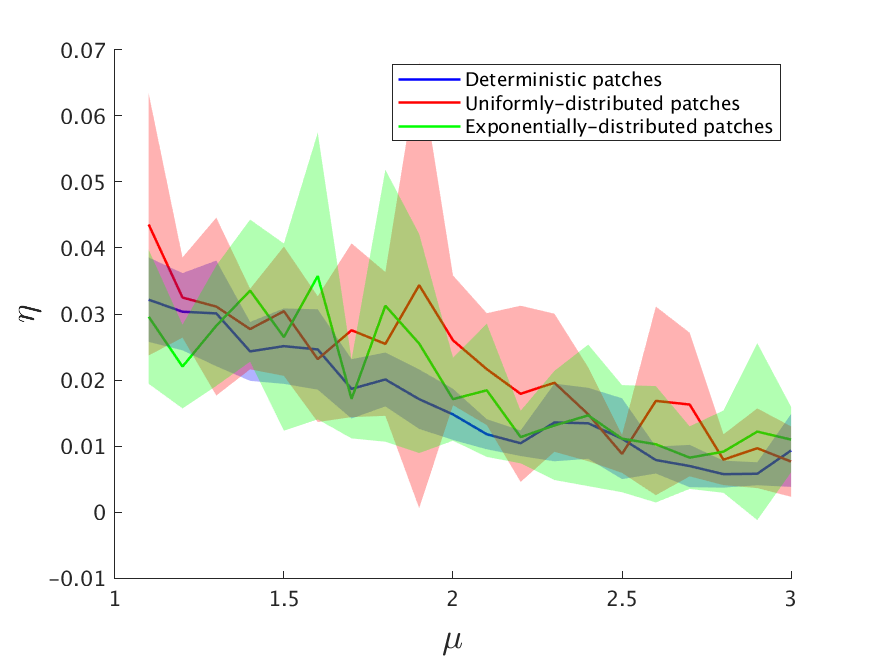
\includegraphics[width=.50\textwidth]{EffectOfTargetDist1D_D_PowerLaw_5found-10reps}\label{fig:EffectOfTargetDist1D_PowerLaw_D_base}}\hfill
	\subfloat[{$5$ targets found, repeated $50$ times}]{%
		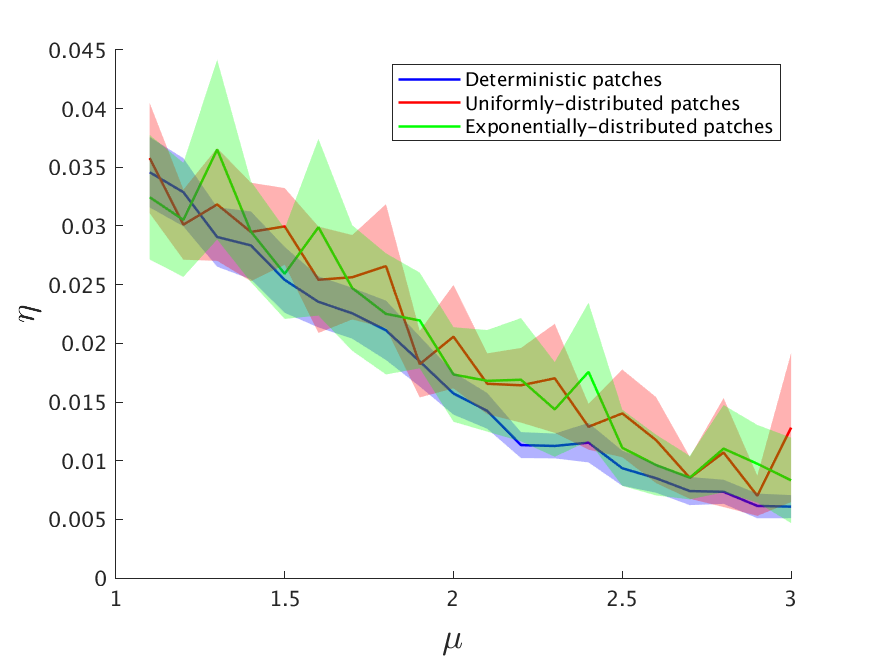
\includegraphics[width=.50\textwidth]{EffectOfTargetDist1D_D_PowerLaw_5found-50reps}\label{fig:EffectOfTargetDist1D_PowerLaw_D_morereps}}\\
	\subfloat[$50$ targets found, repeated $10$ times]{%
		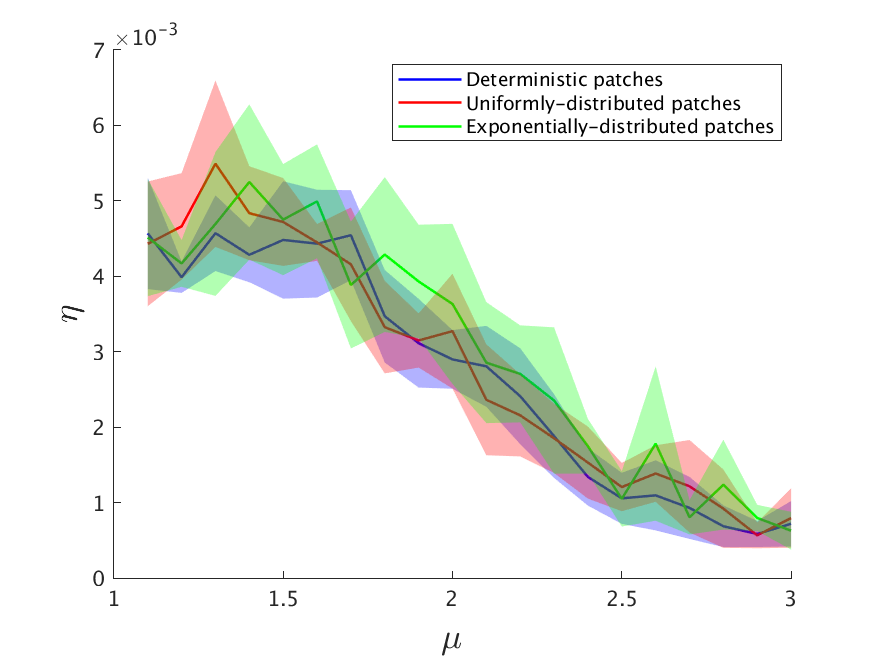
\includegraphics[width=.50\textwidth]{EffectOfTargetDist1D_D_PowerLaw_50found-10reps}\label{fig:EffectOfTargetDist1D_PowerLaw_D_morefound}}\hfill
	\subfloat[$50$ targets found, repeated $200$ times]{%
		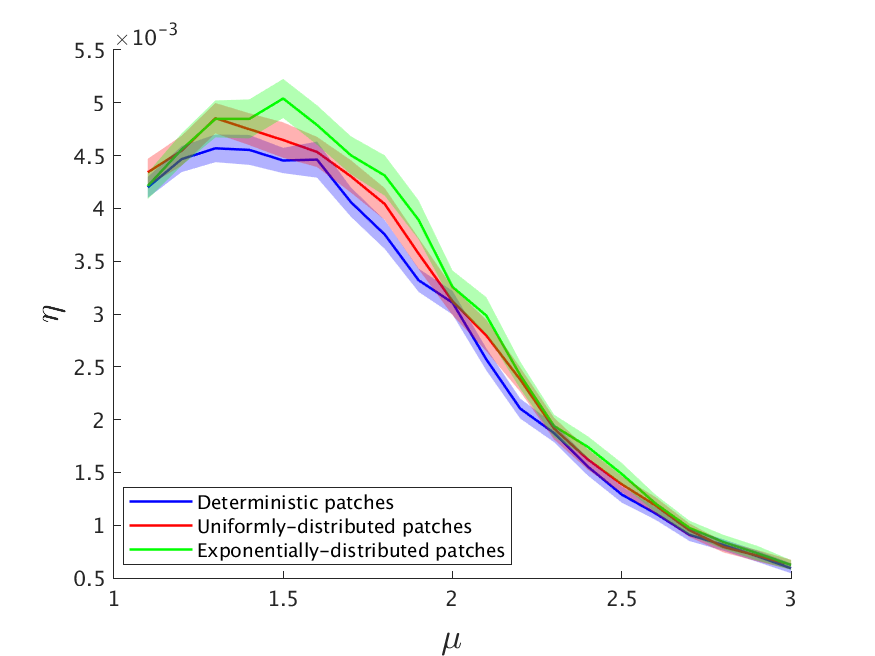
\includegraphics[width=.50\textwidth]{EffectOfTargetDist1D_D_PowerLaw_50found-200reps}\label{fig:EffectOfTargetDist1D_PowerLaw_D_moreboth}}
	\caption[Mean efficiency of an unbounded power-law strategy for three different target distributions for a different numbers of repetitions and targets to be found]{The mean efficiency of a random walk search strategy with a power-law step-length distribution, with parameter ranging from $1.1 \leq \mu \leq 3$ over $20$ equispaced values, for destructive foraging ($x_0=\lambda/2$) and with three different target distributions: deterministic, uniform, and exponential, each with an average distance between targets of $\lambda = 20$, and a radius of vision, $r_v=1$. Each subplot ran the simulation for a different number of repetitions and had a different requirement on the number of targets to find.}\label{fig:EffectOfTargetDist1D_PowerLaw_D}
\end{figure}

Looking first at \cref{fig:EffectOfTargetDist1D_PowerLaw_D_base}, there is clearly a large variance in the mean efficiency across values of $\mu$ for all target distributions. Comparing the distribution types across \cref{fig:EffectOfTargetDist1D_PowerLaw_D_base,fig:EffectOfTargetDist1D_PowerLaw_D_morefound,fig:EffectOfTargetDist1D_PowerLaw_D_morereps}, the exponentially distributed targets seem to have the biggest variance in efficiency, with the uniform and deterministic target distributions seeming to have similar variances to each other. 

The increase in the total targets found per search from \cref{fig:EffectOfTargetDist1D_PowerLaw_D_base} to \cref{fig:EffectOfTargetDist1D_PowerLaw_D_morefound} reduces the variances in our mean efficiency for all three target distributions, although there is still a large spike in the exponentially-distributed targets around $\mu\approx 1.6$. The increase from $5$ targets found to $50$ targets found also reduces the efficiency by a factor of $10$. The efficiency seems to be very similar, if not the same, for the three different target distributions. Similarly, increasing the total number of times that the simulation is repeated from \cref{fig:EffectOfTargetDist1D_PowerLaw_D_base} to \cref{fig:EffectOfTargetDist1D_PowerLaw_D_morereps} smooths out the mean efficiency. The two key differences between repeating more searches versus running longer (in terms of targets) searches, is that when a new search begins the forager is reset to a random point within the first interval, and the targets are regenerated. Whereas after a target is found the animal resumes searching from where it found the target, and the targets become more scarce over time. Increasing the number of targets found seems to have a larger effect on reducing the variance than increasing the number of repetitions. Longer searches are also a more realistic model of the real world, since animals are generally not reset to a new location with a new set of targets.


Finally, in \cref{fig:EffectOfTargetDist1D_PowerLaw_D_moreboth} the number of repetitions is large enough that the efficiency curves are smooth and the confidence intervals are narrow. For $\mu \approx 1$, the efficiency is very similar between distributions, but as $\mu$ increases there is a clear difference in the efficiency between different target distributions. For values of $\mu \approx 3$, there is little if any difference in the efficiency between different target distributions. Therefore, the efficiency of a L\'{e}vy search depends on the distribution of targets, and for ballistic and Brownian searches there is not necessarily a dependence on the target distribution. However, the efficiency only changes slightly between different distributions, and the curves follow roughly the same shape, with the peak efficiency for each curve occurring close to each other. There are analytic models in the literature that allow for different target distributions (e.g. \cite{Bartumeus_2013}), which we could potentially use to extend our model. 

Although the deterministic target assumption will potentially affect the optimal parameters of any search strategy we investigate, the amount of difference between the target distributions seems small enough to justify making the simplification, especially given the relatively large variance in efficiency across multiple searches.


\subsection{Comparing the two different measures of efficiency \label{sec:1D_assumptions:efficiency}}
At the start of \cref{sec:1Dmodel}, we made the claim that optimising the efficiency of a search over the real line was equivalent to optimising the efficiency in finding the first target, given known starting conditions (either $x_0 = r_v$ or $x_0 = \lambda/2$). This claim is made throughout the animal foraging literature (e.g. \cite{Bartumeus_2013}).

Intuitively, as more targets are found the search space becomes more sparse and so the efficiency will decrease, which should mean that the efficiency over multiple targets is less than that of finding a single target. This can also be seen in \cref{fig:EffectOfTargetDist1D_PowerLaw_D_base,fig:EffectOfTargetDist1D_PowerLaw_D_morefound,fig:EffectOfTargetDist1D_PowerLaw_D_morereps,fig:EffectOfTargetDist1D_PowerLaw_D_moreboth} in the previous section, where the efficiency changed depending on how many targets were required to be found throughout each search. The two measures of efficiency are clearly not going to be equal to each other, although our claim is that optimising for either definition is equivalent, meaning that the maximum efficiency under both definitions occurs at the same location.

We define the efficiency of a search that finds $N$ targets as
\begin{equation*}
\eta_N = \frac{N}{L}, 
\end{equation*}
where $L$ is the total distance travelled, and $N$ is the number of targets found throughout the search, where the subscript $N$ is used to make clear the dependence on the number of targets found.

Also recall the notion of efficiency used throughout \cref{sec:1Dmodel}, 
\begin{equation}
\label{eq:1d_assumptions:eta}
\eta = \frac{1}{\E{L}}.
\end{equation}
Note that under this definition of $\eta$, we are assuming a known starting point, as opposed to the $\eta_N$ definition which assumes a random starting location. For the remainder of this section we include the dependence on the starting location explicitly. For destructive foraging,
\begin{equation*}
\eta_{d} = \frac{1}{\E{L(\lambda/2)}},
\end{equation*}
where $L(x)$ represents the total distance to find a target for a search that begins at location $x$. For non-destructive foraging we have
\begin{equation*}
\eta_{n} = \frac{1}{\E{L(r_v)}}.
\end{equation*}
The first case to consider is when the targets are non-destructive. Consider the efficiency across finding $N$ targets, $\eta_N$, assuming that the forager starts at a random location between two targets, which may occur if we were to release an animal at random in some search space. Each time a target is reached, the animal begins its search a distance $r_v$ away from the target in either direction. Since all intervals are statistically equivalent, and due to the symmetry of the step-length distribution, we can without loss of generality assume that the animal continues its search for the next target at location $x_0 = r_v$ in the interval $[0,\lambda]$. The search for the first target is unique in that it can begin at any point in the interval, whereas the searches for each of the remaining $N-1$ targets must begin at the same point, or a statistically equivalent point, since all searches will begin $r_v$ from a target. If we define $L_i(r_v)$ as the distance travelled when finding the $i$th target, beginning from $x=r_v$, as , then we can say that $L_i(r_v)$ for $i \geq 2$ are independent and identically distributed. Using this notation, we may rewrite $\eta_N$ as
\begin{equation*}
\eta_N = \frac{N}{L_1(\lambda/2) + L_2(r_v) + \dots + L_N(r_v)}.
\end{equation*}
When $N$ is large, the random variable $L_1$ has a relatively small impact on the denominator, and so through the strong law of large numbers we know that
\begin{equation*}
\lim_{N \to \infty} \eta_N = \frac{1}{\E{L_2(r_v)}} \text{ a.s.}
\end{equation*}

That is, for a non-destructive search, the long-term efficiency is the reciprocal of the expected distance travelled in a single search that begins at $r_v$. This is the same as our definition of $\eta$. We can consider $\eta_N$ as the sample efficiency, which converges to $\eta$, the efficiency. In \cref{fig:EtaVsEtaN_PowerLaw_ND} we plot both $\eta$ and $\eta_N$ for a range of $N$ to further demonstrate this. The large $N$ gets, the closer $\eta_N$ gets to $\eta$.

\begin{figure}[h!]
	\centering
	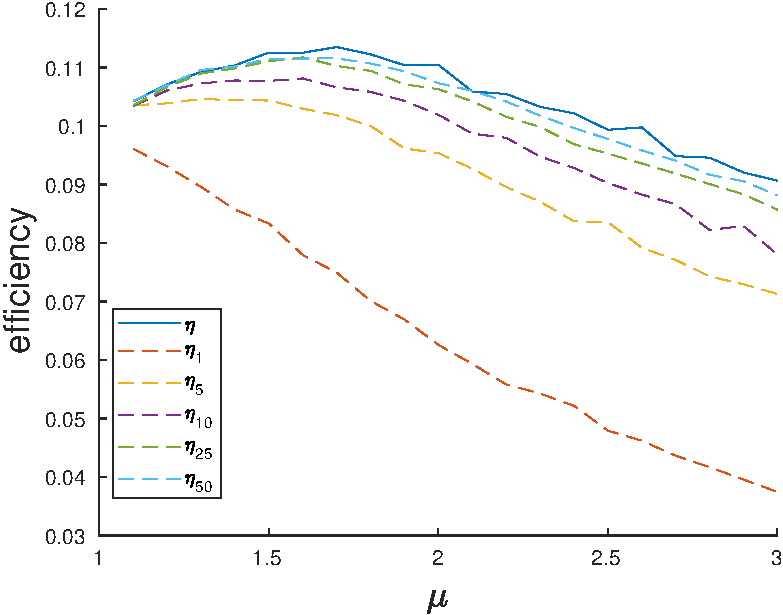
\includegraphics[scale=0.68]{EtaVsEtaN_PowerLaw_ND_reps5000}
	\caption[Two different definitions of the efficiency, $\eta$ and $\eta_N$, compared to each other for non-destructive foraging]{The efficiency, $\eta$, as defined in \cref{eq:1d_assumptions:eta} versus $\eta_N$ plotted for a range of search lengths, $N=\{1,5,10,25,50\}$, for non-destructive foraging ($x_0 = r_v$ for $\eta$ calculation) with $\lambda=20$, $r_v=1$, and $\lmin = 1$. Efficiency is averaged over $5000$ simulations. The larger $N$ is, the closer $\eta_N$ is to $\eta$. \label{fig:EtaVsEtaN_PowerLaw_ND}}
\end{figure}


For the case of destructive foraging, an analytic argument is not as simple because as targets get more sparse, the starting location of the forager will depend on which targets have been destroyed. Instead, we simulate $\eta_N$ and $\eta$ for the destructive foraging case in \cref{fig:EtaVsEtaN_PowerLaw_D}. Although $\eta_N$ is clearly different to $\eta$, and there does not seem to be convergence as $N$ increases, we can still note that the peak efficiency occurs at the same location for both $\eta$ and $\eta_N$.

\begin{figure}[h!]
	\centering
	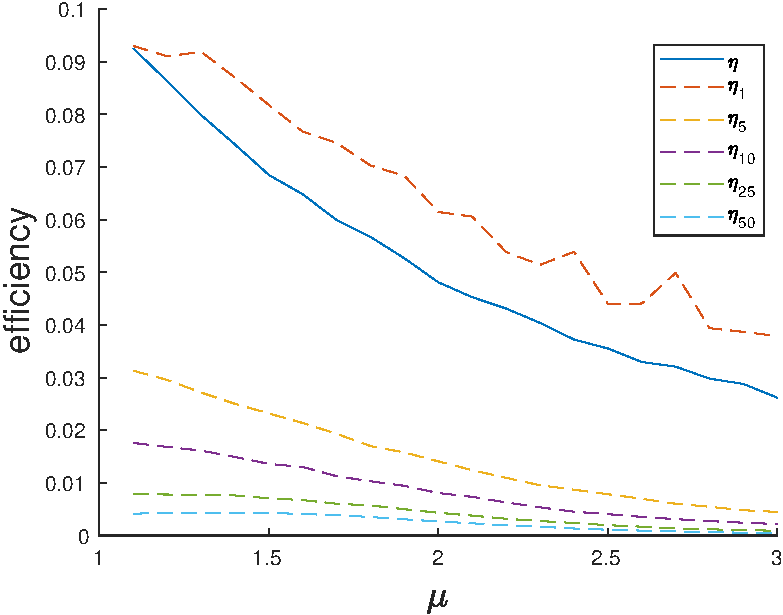
\includegraphics[scale=0.68]{EtaVsEtaN_PowerLaw_D_reps500}
	\caption[Two different definitions of the efficiency, $\eta$ and $\eta_N$, compared to each other for non-destructive foraging]{The efficiency, $\eta$, as defined in \cref{eq:1d_assumptions:eta} versus $\eta_N$ plotted for a range of search lengths, $N=\{1,5,10,25,50\}$, for destructive foraging ($x_0 =\lambda/2$ for $\eta$ calculation) with $\lambda=20$, $r_v=1$, and $\lmin = 1$. Efficiency is averaged over $5000$ simulations. The only difference between $\eta$ and $\eta_1$ is that the former begins at $x_0=\lambda/2$ whereas the latter begins at a uniformly distributed location within $[0,\lambda]$. \label{fig:EtaVsEtaN_PowerLaw_D}}
\end{figure}

\end{chapter}


% Chapter 4: Discretization
\begin{chapter}{Discretisation of the one-dimensional search space\label{sec:1d_discrete}}
%!TEX root = ../thesis.tex
We stated at the end of \cref{sec:1dRW_distance,sec:1dRW_steps,sec:1dMMRW_distance,sec:1dMMRW_steps} that the exact analytic solutions we found for the expected total cost cannot feasibly be solved for any realistic choice of step-length distribution. In this section we outline how we may numerically solve these expressions via a spatial discretisation.

The discretisation of the unmodulated random walk in \cref{sec:1d_discrete:RW} once again can mostly be accredited to Bartumeus \etal \cite{Bartumeus_2013}. However, we also derive a numerical approximation for \cref{eq:1dRW_cost:EV2_neumann}, an expression which avoids having to use properties of the Dirac delta function, and hence is valid for any distribution of starting locations. Bartumeus \etal \cite{Bartumeus_2013} made the claim that the use of the Dirac delta was a crucial step in their derivation, but the existence of our expression --- which has comparable computational efficiency --- shows that this is not true. 

The discretisation of the Markov-modulated random walk builds upon \cref{sec:1d_discrete:RW} in much the same way that \cref{sec:1dMMRW} built upon \cref{sec:1dRW}. We are ultimately able to derive a simple expression for the cost of a Markov-modulated random walk, which amounts to solving a system of equations, which we solve using Matlab in \cref{sec:1d_results}. We also derive an alternative expression which avoids needing to know the initial location of a forager.

It is perhaps possible to argue that we could simply replace the functions and operators in the final analytic expressions with their discretised equivalents, resulting in the same numerical expressions found in this section. We opt, however, to demonstrate the derivation of the numerical expressions in full, to ensure correctness, as well as being able to shed some more light on some of the issues found in the derivation of the analytic expressions, such as in deriving the cost for a single state of a Markov-modulated random walk.

\section{Notation and assumptions\label{sec:1d_discrete:notation}}

The continuous search space $[0,\lambda]$ is replaced with a set of discrete positions at which the forager can be located. The positions are a distance $\Delta x$ apart, and we denote the discretised point corresponding to $x=\lambda$ as $M$. Hence, the possible locations all take the form $j\Delta x$ with $j=0,1,\dots,M$. The discretisation length, $\Delta x$, is assumed to be much smaller than any of the original model parameters ($\lmin,\lmax,r_v,\lambda$).

Then, discrete approximations of the model parameters are obtained with
\[\lmin = m_0 \Delta x, \quad \lmax = m_m \Delta x, \quad r_v = m_r \Delta x, \quad m_0,m_m,m_r \in \mathbb{Z}. \]

The set of location variables $\{x_0,x_1,\dots,x_{n}\}$, which correspond to steps~$\{0,1,\dots,n-1,n\}$, correspond to steps ending at points $\{i_0,i_1,\dots,i_n\}$, where $x_m = i_m \Delta x$. %Note that points in continuous space are rounded to the discrete point below if they aren't already an integer multiple of $\Delta x$. This problem shrinks as $\Delta x \to 0$.

We use the notation $[\rho_n]_i$, $[h]_i$, and $\E{Q}_{i}$ to represent the functions $\rho_n(x)$ and $h(x)$, $\E{Q(x)}$ respectively, evaluated at the point $x=i \Delta x$. Then, $[\rho_n]$, $[h]$, and $\E{Q}$ are vectors used to denote the functions evaluated at every point in the discretised search space. Similarly, for the Markov-modulated case we use $[\rho_{n,j}]$, $[h_j]$, and $\E{Q_j}$ to denote the vector of discretised functions $\rho_{n,j}(x)$, $h_j(x)$, and $\E{Q_j(x)}$. We break with the convention of using boldface to denote vectors to be consistent with previous work \cite{Bartumeus_2013}, and since we use boldface to differentiate between the unmodulated and Markov-modulated versions of various quantities.

In discrete space, we represent the step-length distribution $p(\ell)d\ell$ using the matrix $A$. In continuous space we had $p(x_{m+1}-x_m)dx_m$, which corresponds to the probability of reaching location $x_{m+1}$ in a step starting from $x_m$, on the $(m+1)$th step. This is a jump of length $\left| x_{m+1} - x_m \right|$ which becomes $\left|i_{m+1} - i_m \right| \Delta x$ in the discretised space, which we denote as $[A]_{i_m,i_{m+1}}$. However, we must also take into account step-lengths that in continuous space are not integer multiples of~$\Delta x$, which we do by integrating over all continuous values that will result in the same discrete value when discretised. Thus, we can find each element of $A$ using
\begin{equation}
\label{eq:1d_discrete:A_matrix_integral}
[A]_{j,k} = \int_{|j-k|\Delta x}^{(|j-k|+1)\Delta x} p(\ell) d\ell, \quad k \neq j.
\end{equation}
Due to the symmetry of the jump probabilities, $[A]_{j,k} = [A]_{k,j}$ and hence the matrix $A$ is symmetric. We require that every jump is greater than the minimum jump size, and so $[A]_{j,k} = 0$ for $|j - k| < m_0$. For step-length distributions with a finite $\lmax$, we also require $[A]_{j,k}=0$, for $|j-k| \geq m_m$. Expressions for the matrix $A$ based on \cref{eq:1d_discrete:A_matrix_integral} are found for a variety of step-length distributions in \cref{app:calc}. Similarly, for the Markov-modulated case we define $\Amat$, which is made up of submatrices denoted $A_i$, each representing the step probabilities while $Z$ is in state $i$. Thus, the elements of $A_i$ are found in the same way as matrix $A$, with $p_i(\ell)$ and the corresponding values of $m_0$ and $m_m$.

In the discrete approximation, an integral over the continuous space becomes a sum over the discrete index. However, whether or not the end points are included in the summation is an important question which was not addressed in the continuous model, since the inclusion of endpoints make no difference when integrating. Our integrations over the continuous search space represented all of the possible points at which the forager was still searching for a target, and so the end points should not included, as these are where the forager would be able to detect the food. When the discrete radius of vision is $m_r$, the points from $m_r+1$ to $(M-m_r-1)$ are the locations where food hasn't yet been detected. Thus for an integral over $[r_v,\lambda-r_v]$, the equivalent summations are all from $m_r+1$ to $M-m_r-1$, rather than $m_r$ to $M-m_r$.  Thus, the effective search interval has a length of $(M-m_r-1) - (m_r+1)+1 = M-2m_r-1$, and so the matrix $A$ should have dimensions $(M-2m_r-1)\times(M-2m_r-1)$.

However, we instead define $A$ to be an $(M-1)\times(M-1)$ matrix, by putting an outside layer of zeros --- of width $m_r$ --- on each side. This way, the $(i,j)$th element of $A$ will correspond to the probability of moving from the $i$th point in the search space to $j$th point. Similarly, the vector $[h]$ has a length of $M-2m_r-1$ for its non-zero elements, but we say $[h]$ has length $M-1$, with $m_r$ zeros on each end. Note that although we are only considering points within the search space, the forager may jump from within the search space to outside it, and thus the row sums of $A$ will not necessarily equal $1$. For the Markov-modulated case, the radius of vision may vary across states, so the dimensions of the non-zero elements of each $A_i$ may vary across each state. Each matrix $A_i$ will have the same dimensions as $A$, although the amount that the matrix needs to be padded with zeros will depend on the radius of vision in the corresponding state.

In deriving the analytic expressions for the expected total cost, we used the property of the Dirac delta function that
\begin{equation*}
\int_{r_v}^{\lambda-r_v} \delta(x-a)dx = 1,
\end{equation*}
which in the discrete approximation becomes
\begin{equation*}
\sum_{j=m_r+1}^{M-m_r-1}\delta_{j,i_a} = 1,
\end{equation*}
where $\delta_{j,i_a}$ is the Kronecker delta. The point $i_a$ is the discretisation of the initial location $x_0=a$, and so $i_a$ is $a/\Delta x$ rounded to the nearest integer. 

\section{Discretised expressions for a random walk strategy \label{sec:1d_discrete:RW}}

Recall from \cref{sec:1d_discrete:RW} that we were able to write $\rho_n(x_n)$, the density function for the position of the animal at the end of the $n$th step, as an expression involving $\rho_{n-1}(x_{n-1})$, 
\begin{equation*}
\rho_n(x_n) = \int_{r_v}^{\lambda-r_v} \rho_{n-1}(x_{n-1}) p(x_n-x_{n-1}) dx_{n-1},
\end{equation*}
which applied recursively becomes
\begin{equation*}
\rho_n(x_n) = \int_{x_{n-1}=r_v}^{\lambda-r_v} \dots \int_{x_0 = r_v}^{\lambda-r_v} \rho_{0}(x_0) \prod_{i=0}^{n-1} p(x_{i+1}-x_{i}) dx_{i}.
\end{equation*}
Replacing the integrals with their equivalent summations, we use this to find an expression for $\rho_n$ in the discrete approximation, which is
\begin{equation*}
[\rho_n]_{i_n} = \sum_{i_0=m_r+1}^{M-m_r-1} \cdots \sum_{i_{n-1}=m_r+1}^{M-m_r-1} [A]_{i_{n-1},i_{n}} [A]_{i_{n-2}.i_{n-1}} \dots [A]_{i_1,i_2}[A]_{i_0,i_1} [\rho_0]_{i_0},
\end{equation*}
where $[\rho_0]$ is the vector representing the function $\rho_0$, as described in \cref{sec:1d_discrete:notation}. 
Since the outer elements of the matrix $A$ are $0$, we can rewrite this as
\begin{equation}
\label{eq:1d_discrete:rho_summation}
[\rho_n]_{i_n} = \sum_{i_0=1}^{M-1} \cdots \sum_{i_{n-1}=1}^{M-1} [A]_{i_{n-1},i_{n}} [A]_{i_{n-2}.i_{n-1}} \dots [A]_{i_1,i_2}[A]_{i_0,i_1} [\rho_0]_{i_0}.
\end{equation}

The sequence of products of elements of $A$ in \cref{eq:1d_discrete:rho_summation} correspond to matrix products. Thus, we can rewrite it as
\begin{equation}
\label{eq:1d_discrete:rho_matrix}
[\rho_n]_{i_n} = \sum_{i_0=1}^{M-1} [A^n]_{i_0,i_n}[\rho_0]_{i_0}.
\end{equation}


\begin{theorem}
	The expectation of the total cost of a random walk in the discrete approximation is given by
	\begin{equation}
	\label{eq:1d_discrete:EQ_sum}
	\E{Q} = \sum_{n=0}^\infty A^n [h],
	\end{equation}
	where $\E{Q}$ is a vector of length $(M-1)$, with each element representing a different starting point for the forager.
\end{theorem}
\begin{proof}
Recall from \cref{thm:1dRW_cost:EV}, for the non-Markov-modulated random walk, the expectation of the total cost was given by
\begin{equation*}
\E{Q(x_0)} = \sum_{n=0}^\infty \int_{r_v}^{\lambda-r_v} \rho_n(x_n) h(x_n)dx_n,
\end{equation*}
where $h(x_n) = \mathbb{E}_{X_{1}|X_0} \left[ q(X_1,X_{0}) \mid X_0 = x_n \right]$.
In the discrete approximation, this becomes
\begin{equation*}
\E{Q}_{i_0} = \sum_{n=0}^\infty \sum_{i_n=m_r+1}^{M-m_r-1} [\rho_n]_{i_n} [h]_{i_n} \Delta x,
\end{equation*}
where $\E{Q(x_0)}_{i_0}$ represents the expected total cost of a random walk beginning at point $i_0$, and $[h]$ is the discretised vector of the function $h$, and thus is a vector with each element being given by the function $h$ represented at a discrete point in the search space. Although there is no $i_0$ on the right-hand side of the equation, the dependence on $i_0$, along with $i_1, i_2, \dots$ is implicit in the vector $[\rho_n]$, as we shall next see.

Substituting in our expression for $[\rho_n]_{i_n}$ from \cref{eq:1d_discrete:rho_matrix}, as well as using the fact that the first $m_r$ and last $m_r$ elements of $[h]$ are $0$, we get
\begin{equation}
\label{eq:1d_discrete:an_rho_h}
\E{Q}_{i_0} = \sum_{n=0}^\infty \sum_{i_n=1}^{M-1} \sum_{i_0=1}^{M-1} [A^n]_{i_0,i_n}[\rho_0]_{i_0} [h]_{i_n} \Delta x.
\end{equation}
Since the initial distribution is known to be $\rho_0(x) = \delta(x-a)$, and combining this with the $\Delta x$ term,  we get a Kronecker delta,
\begin{equation*}
\E{Q}_{i_a} = \sum_{n=0}^\infty \sum_{i_n=1}^{M-1} \sum_{i_0=1}^{M-1} [A^n]_{i_0,i_n} \delta_{i_0,i_a} [h]_{i_n}.
\end{equation*}
Summing over the $i_0$ terms and using the corresponding property of the Kronecker delta we get
\begin{equation*}
\E{Q}_{i_a} = \sum_{n=0}^\infty \sum_{i_n=1}^{M-1} [A^n]_{i_a,i_n} [h]_{i_n},
\end{equation*}
which can be written as a matrix expression
\begin{equation*}
\E{Q} = \sum_{n=0}^\infty A^n [h].
\end{equation*}
\end{proof}

As mentioned above, the vector $[h]$ is found by evaluating $h(x)$ at every point in the discretised search space. For the average distance travelled  we use \cref{eq:1dRW_dist:l_integralsv2} or for the number of steps taken, we use $[h] = \vec{1}$.

Unfortunately, when evaluating \cref{eq:1d_discrete:EQ_sum} we still have an infinite sum to deal with, and so evaluating this to a reasonable degree of accuracy may be slow since we have to calculate each term in the summation until the result has converged sufficiently. As with our analytic expression, we can express this without the infinite summation by considering it as a Neumann series and using properties based on this. This time, instead of $\L$, we have matrix $A$ as our operator. For the continuous case we split the proof over  \cref{thm:1dRW_cost:Q_operator_norm_lmax,thm:1dRW_cost:Q_operator_norm_Lk,thm:1dRW_cost:Q_operator_norm_recursive,thm:1dRW_cost:Q_operator_norm}, whereas we do this for the discrete approximation in a single combined \lcnamecref{thm:1d_discrete:operator_norm}.

\begin{lemma}
\label{thm:1d_discrete:operator_norm}
$\normop{A} < 1$, where $\normop{\cdot}$ is the operator norm given by
\begin{equation*}
\normop{A} = \sup \left\{ \frac{\norm{A v}}{\norm{v}}:  \norm{v} \neq 0 \right\}, 
\end{equation*}
with $\norm{\cdot}$ being the maximum column sum.
\end{lemma}
\begin{proof}
For some matrix $v$, with dimensions $(M-1) \times p$, where $p \in \mathbb{N}$, we use the norm given by
\begin{equation*}
\norm{v} = \max_{j=1,\dots p}  \sum_{i=1}^{M-1} \abs{v_{i,j}}=:C.
\end{equation*}

Element $(i,j)$ of the matrix $A v$ is given by
\begin{equation*}
[Av]_{i,j} = \sum_{k=1}^{M-1} A_{i,k} v_{k,j},
\end{equation*}
and so $A v$ has norm
\begin{align*}
\norm{Av} &= \max_{j=1,\dots,p} \sum_{i=1}^{M-1} \left| \sum_{k=1}^{M-1} \abs{A_{i,k} v_{k,j}} \right| \\
&\leq \max_{j=1,\dots,p} \sum_{i=1}^{M-1} \sum_{k=1}^{M-1} \abs{A_{i,k} v_{k,j}}\\
&= \max_{j=1,\dots,p}  \sum_{k=1}^{M-1} \abs{v_{k,j}} \sum_{i=1}^{M-1} \abs{A_{i,k}}.
\end{align*}
where the second line has equality if and only if $v_{k,j} \geq 0$ for all $k$ and $j$ from $1$ to $M-1$.
%where the second line follows from the fact that $A_{i,j}=0$ for any $i,j \notin \{m_r+1,m_r+2,\dots,M-m_r-1\}$.

Now, consider the summation over $\left| A_{i,k} \right|$ individually. Recalling the definition of $A_{i,j}$ from \cref{eq:1d_discrete:A_matrix_integral}, and separating the summation into steps to either the left or the right, we can write
\begin{align*}
\sum_{i=1}^{M-1} \left|A_{i,k} \right| &= \sum_{i=1}^{k-1} A_{i,k} + \sum_{i=k+1}^{M-1} A_{i,k}\\
&=\sum_{i=1}^{k-1} \int_{\left|i-k\right|\Delta x}^{\left(\left|i-k\right|+1\right)\Delta x} p(\ell) d\ell + \sum_{i=k+1}^{M-1} \int_{\left|i-k\right|\Delta x}^{\left(\left|i-k\right|+1\right)\Delta x} p(\ell) d\ell ,
\end{align*}
where the $i=k$ term in the summation is dropped since it is always $0$.
These integrals can be combined to give
\begin{align*}
\sum_{i=1}^{M-1} \left|A_{i,k} \right| &= \int_{\Delta x}^{(k)\Delta x} \left|p(\ell) \right| d\ell + \int_{\Delta x}^{(M-k)\Delta x} \left| p(\ell) \right| d\ell.
\end{align*}
Letting $x = k \Delta x$ and combining into a single integral, we get
\begin{equation*}
\sum_{i=1}^{M-1} \left|A_{i,k} \right| \leq \int_{0}^\lambda p(x-x')dx'=: C^*,
\end{equation*}
with the inequality coming from the fact that there are some points between $(M-1)\Delta x$ and $M \Delta x$ that are being integrated over. The right hand side is the same as in the proof of \cref{thm:1dRW_cost:Q_operator_norm_lmax}, with $r_v = 0$. Following the same reasoning, the right hand size is less than or equal to $1$ if $\lmax < x < \lambda-\lmax$ and strictly less than $1$ otherwise. This tells us
\begin{equation*}
\frac{\norm{A v}}{\norm{v}} \leq \frac{C^*}{C} < 1 \implies \normop{A}<1,
\end{equation*}
when $\lmax > \lambda/2$.
Further, if we instead consider $A^n v$ for some $n\geq 1$, then
\begin{align*}
\norm{A^n v} &= \max_{j=1,\dots,p} \sum_{i=1}^{M-1} \sum_{k_1=1}^{M-1} \sum_{k_2=1}^{M-1}  \dots \sum_{k_n=1}^{M-1} \left| A_{i,k_n}A_{k_{n},k_{n-1}}\cdots A_{k_2,k_1} v_{k_1,j} \right|\\
&= \max_{j=1,\dots,p}  \sum_{k_1=1}^{M-1} \left| v_{k_1,j}\right|  \sum_{k_2=1}^{M-1} \left| A_{k_2,k_{1}}\right|  \dots \sum_{k_n=1}^{M-1}  \left| A_{k_n,k_{n-1}}\right| \sum_{i=1}^{M-1} \left| A_{i,k_n}\right|\\
&\leq \max_{j=1,\dots,p}  \sum_{k_1=1}^{M-1} \left| v_{k_1,j}\right|  \sum_{k_2=1}^{M-1} \left| A_{k_2,k_{1}}\right|  \dots \sum_{k_n=1}^{M-1}  \left| A_{k_n,k_{n-1}}\right| \int_{0}^{\lambda} p(x_i-x_{k_n})dx_{k_n}\\
&\leq \sum_{k_1=1}^{M-1} \int_{r_v}^{\lambda} \cdots \int_{0}^{\lambda} \prod_{i=0}^{n-1} p(x_{i+1}-x_i)dx_i =:D\\
&\leq \max_{j=1,\dots p} \sum_{k_1=1}^{M-1} \abs{v_{{k_1},j}} = \norm{v}.
\end{align*}
Then, referring back to the $n=1$ case above, as well as \cref{thm:1dRW_cost:Q_operator_norm_Lk}, we see that the only situation in which we may not have a strict inequality in the final line will be when $\lmax \geq \frac{\lambda }{2^k}$, and so we can conclude that 
\begin{equation*}
\frac{\norm{A^nv}}{\norm{v}} \leq \frac{D}{C} < 1 \implies \normop{A^n}<1
\end{equation*}
for $\lmax < \frac{\lambda}{2^k}$. We can choose an $n$ such that $\normop{A^n}<1$ for every possible $\lmax$. Then, we choose $n^* = 2^n$ and as we did in \cref{thm:1dRW_cost:Q_operator_norm_recursive}, we can show that $\normop{A^n}<1$ implies $\normop{A}<1$, where we have used the fact that $A$ is a is a self-adjoint operator since it is symmetric. Thus, we conclude that $\normop{A}<1$ for every possible step-length distribution.
\end{proof}

\begin{theorem}
	In the discrete approximation, the expected total cost of a random walk is given by
\begin{equation*}
\E{Q} = (\identity - A)^{-1} [h],
\end{equation*}	
where the $i$th element of the vector $\E{Q}$ represents the expected total cost of a walk that starts at point $i$.
\end{theorem}
\begin{proof}
	Considering $\sum_{n=0}^\infty A^n$ as a Neumann series and using \cref{thm:1d_discrete:operator_norm}, we can write $\sum_{n=0}^\infty A^n$ as $(\Id - A)^{-1}$, where $\Id$ is the identity operator, which in this case is the $(M-1)\times(M-1)$ identity matrix, $\identity$. Substituting this into \cref{eq:1d_discrete:EQ_sum}, we get
	\begin{equation*}
\E{Q} = (\identity - A)^{-1} [h].
	\end{equation*} 
\end{proof}

Note that this expression is equivalent to solving the system $(\identity - A)x = h$. We can solve this in Matlab using \begin{verbatim}
Q = (I-A) \ h;
\end{verbatim}

Recall from \cref{sec:1dRW_cost}, there was also an alternate expression for the expected total cost, \cref{eq:1dRW_cost:EV2_neumann},
\begin{equation*}
\E{Q(x_0)} = \int_{r_v}^{\lambda-r_v} [(\Id - \L)^{-1} \rho_0](x_n) h(x_n) dx_n.
\end{equation*}
We can derive a discrete space equivalent of this expression in a similar way.

\begin{theorem}
	In the discrete approximation, the expected total cost of a random walk is given by
	\begin{equation*}
	\E{Q} = \left[ (\identity - A)^{-1} [\rho_0] \right][h],
	\end{equation*}
	with $\E{Q}$ having dimensions $(M-1)\times(M-1)$ and $[\rho_0]$ and $[h]$ taken to be column and row vectors, respectively.
\end{theorem}
\begin{proof}
Beginning with \cref{eq:1d_discrete:an_rho_h},
\begin{equation*}
\E{Q} = \sum_{n=0}^\infty \sum_{i_n=1}^{M-1} \sum_{i_0=1}^{M-1} [A^n]_{i_0,i_n}[\rho_0]_{i_0} [h]_{i_n} \Delta x,
\end{equation*}
and using the fact that the matrix $A$ is symmetric, we get
\begin{equation*}
\E{Q} = \sum_{n=0}^\infty \sum_{i_n=1}^{M-1}  \left[ A^n [\rho_0] \right]_{i_n} [h]_{i_n} \Delta x.
\end{equation*}
Using \cref{thm:1d_discrete:operator_norm}, we can rewrite the infinite summation $\sum_{n=0}^\infty A^n$ to get
\begin{equation*}
\E{Q} = \sum_{i_n=1}^{M-1}  \left[ (\identity - A)^{-1} [\rho_0] \right]_{i_n} [h]_{i_n} \Delta x.
\end{equation*}
Finally, writing this as a matrix multiplication, we get
\begin{equation*}
\E{Q} = \left[ (\identity - A)^{-1} [\rho_0] \right][h].
\end{equation*}
\end{proof}	

As before, we can solve this in Matlab using
\begin{verbatim}
Q = ( (I-A) \ rho0 ) * h;
\end{verbatim}
where $Q$ is a $(M-1)\times (M-1)$ matrix since $\rho_0$ is a column vector and $h$ is a row vector.
%!TEX root = ../thesis.tex

\section{Discretised expressions for a Markov-modulated random walk strategy }
\label{sec:1d_discrete:MMRW}
The discretisation of the Markov-modulated case follows similarly. Recalling \cref{eq:1dMMRW_cost:rho_single_recursion},
\begin{equation*}
\rho_{n,j}(x_n) = \sum_{i=1}^J \int_{r_{i}}^{\lambda-r_{i}} p_i(x_n-x_{n-1}) \rho_{n-1,i}(x_{n-1}) P_{i,j} dx_{n-1},
\end{equation*}
and applying recursively, we get
\begin{equation}
\label{eq:1d_discrete:MMRW:rho_recursive}
\rho_{n,j_n}(x_n) = \sum_{j_{n-1}=1}^J \cdots \sum_{j_{0}=1}^J \int_{r_{j_{n-1}}}^{\lambda-r_{j_{n-1}}} \cdots \int_{r_{j_0}}^{\lambda-r_{j_0}}  \rho_{0,j_0}(x_0) \left[ \prod_{k=0}^{n-1} p_{j_{k}}(x_{k+1} - x_k) P_{j_k,j_{k+1}} dx_i\right] .
\end{equation}
As discussed in the unmodulated case, integrals become summations in the discrete approximation. Therefore, \cref{eq:1d_discrete:MMRW:rho_recursive} becomes
\begin{equation*}
[\rho_{n,j_n}]_{i_n} = \sum_{j_{n-1}=1}^J \cdots \sum_{j_{0}=1}^J \sum_{i_{n-1}=m_{j_{n-1}}+1}^{M-m_{j_{n-1}}-1} \cdots \sum_{i_0=m_{j_0}+1}^{M-m_{j_0}-1}  [\rho_{0,j_0}]_{i_0} \left[ \prod_{k=0}^{n-1} [A_{j_{k}}]_{i_k,i_{k+1}} [P]_{j_k,j_{k+1}} dx_i\right] .
\end{equation*}
We can rewrite this as
\begin{equation}
\label{eq:1d_discrete:MM_rho_sums}
[\rho_{n,j_n}]_{i_n} = \sum_{j_{n-1}=1}^J \cdots \sum_{j_{0}=1}^J \sum_{i_{n-1}=1}^{M-1} \cdots \sum_{i_0=1}^{M-1}  [\rho_{0,j_0}]_{i_0} \left[ \prod_{k=0}^{n-1} [A_{j_{k}}]_{i_k,i_{k+1}} [P]_{j_k,j_{k+1}} dx_i\right] 
\end{equation}
since the additional summation terms now included are zero anyway due to the structure of the $A_j$ matrices. We can rewrite the $\rho_{0,j}$ vectors as a single vector by concatenating them to form the vector $[\rho_0]$. That is,
\begin{equation*}
[\rho_0] = ([\rho_{0,1}],\dots,[\rho_{0,J}])^\top,
\end{equation*}
 Then, the element $[\rho_{0,j}]_i$ is equivalent to $[\rho_0]_{(j-1)(M-1)+i}$, and similarly for $\rho_1$, $\rho_2$, etc. Just as we did with the unmodulated case, we can express \cref{eq:1d_discrete:MM_rho_sums} as a matrix product:
\begin{equation}
\label{eq:1d_discrete:MM_rho_matrix}
[\rho_{n,j_n}]_{i_n} = \sum_{j_0 = 1}^J \sum_{i_0=1}^{M-1} [\rho_{0,j_0}]_{i_0} [(\Amat^n)_{j_0,j_n}]_{i_0,i_n},
\end{equation}

where the matrix $\Amat$ is given by
\begin{equation*}
\Amat =\begin{pmatrix}
[A_1] P_{1,1} & [A_1]P_{1,2} & \cdots & [A_1] P_{1,J} \\
[A_2]P_{2,1} & [A_2]P_{2,2} & \cdots & [A_2]P_{2,J} \\
\vdots  & \vdots  & \ddots & \vdots  \\
[A_J]P_{J,1} & [A_J]P_{J,2} & \cdots & [A_J]P_{J,J} 
\end{pmatrix},
\end{equation*}
where each $A_j$ matrix has size $(M-1) \times (M-1)$, so the matrix $\Amat$ must have size $J(M-1) \times J(M-1)$. The expression $[(\Amat^n)_{j_0,j_n}]_{i_0,i_n}$ represents the $(i_0,i_n)$th element of the $(j_0,j_n)$th submatrix of $\Amat$.

Recall from \cref{thm:1dMMRW_cost:EV_Qj}, the cost incurred in a given state $j$ is
\begin{equation*}
\E{Q_j(a)} = \sum_{n=0}^\infty \int_{r_v}^{\lambda-r_v} \rho_{n,j}(x_n) h_j(x_n) dx_n,
\end{equation*}
which in the discretised search space becomes
\begin{equation*}
\E{Q_j}_{i_a} = \sum_{n=0}^\infty \sum_{i_n = 1}^{M-1} [\rho_{n,j}]_{i_n} [h_j]_{i_n} \Delta x.
\end{equation*}

Substituting the expression for $[\rho_{0,j}]_{i_n}$ from \cref{eq:1d_discrete:MM_rho_matrix}, we get
\begin{equation}
\label{eq:1d_discrete:Qj_predelta}
\E{Q_j}_{i_a} = \sum_{n=0}^\infty \sum_{i_n = 1}^{M-1} \sum_{j_0 = 1}^J \sum_{i_0=1}^{M-1}[\rho_{0,j_0}]_{i_0} [(\Amat^n)_{j_0,j}]_{i_0,i_n} [h_j]_{i_n} \Delta x.
\end{equation}

We combine the the initial distribution, $\vec{\rho_0}(x) = \delta(x-a)\vec{z_0}$ with the $\Delta x$ term to obtain a Kronecker delta,
\begin{equation*}
\E{Q_j}_{i_a} = \sum_{n=0}^\infty \sum_{i_n = 1}^{M-1} \sum_{j_0 = 1}^J \sum_{i_0=1}^{M-1}\delta_{j_0,i_0,i_a} z_{0,j_0} [(\Amat^n)_{j_0,j}]_{i_0,i_n} [h_j]_{i_n} \Delta x,
\end{equation*}
where $\delta_{j_0,i_0,i_a}$ is Kronecker delta for $(i_0,i_a)$ in the $j_0$th subvector.
Now, summing over $i_0$ and using the property of the Kronecker delta,
\begin{equation}
\label{eq:1d_discrete:Qj_final}
\E{Q_j}_{i_a} = \sum_{n=0}^\infty \sum_{i_n = 1}^{M-1} \sum_{j_0 = 1}^J \sum_{i_0=1}^{M-1} [(\Amat^n)_{j_0,j}]_{i_a,i_n} [h_j]_{i_n} \Delta x,
\end{equation}
The $\Amat$ term and the $[h]$ term do not constitute a full matrix multiplication, since we are only considering a single value of $j$. This relates back to the issue around \cref{thm:1dMMRW_cost:EV_Qj_sum} and our inability to find a simple expression for the expected cost over a single state. The probability of a forager's location on step $n$ in some state $j$ depends on the location on step $n-1$ in \emph{any} state.

To demonstrate this issue further, we split the $\Amat^n$ term into submatrices, allowing us to write \cref{eq:1d_discrete:Qj_final} as a matrix multiplication. The matrix is split, by
\begin{equation*}
(\Amat^n) =  \begin{pmatrix}
[(\Amat^n)_{1,1}] & [(\Amat^n)_{1,2}] & \cdots & [(\Amat^n)_{1,J}] \\
[(\Amat^n)_{2,1}] & [(\Amat^n)_{2,2}] & \cdots & [(\Amat^n)_{2,J}] \\
\vdots  & \vdots  & \ddots & \vdots  \\
[(\Amat^n)_{J,1}] & [(\Amat^n)_{J,2}] & \cdots & [(\Amat^n)_{J,J}] 
\end{pmatrix},
\end{equation*}
where each $[(\Amat^n)_{i,j}]$ is an $(M-1) \times (M-1)$ submatrix, corresponding to the elements $((i-1)(M-1)+1,(j-1)(M-1)+1)$ up to $(i(M-1),j(M-1))$ of $\Amat^n$. 
That is, $[(\Amat^n)_{i,j}]$ is not the same as $[(\Amat)_{i,j}]^n$, since for some $i,j \in \statespace$, $[(\Amat^2)_{i,j}]$ will actually depend on $[(\Amat)_{i,j}]$ for every $i,j \in \statespace$.
Thus, \cref{eq:1d_discrete:Qj_final} becomes
\begin{equation}
\label{eq:1d_discrete:Qj_final_split}
\E{Q_j}_{i_a} = \sum_{n=0}^\infty  \sum_{j_0 = 1}^J z_{0,j_0}  [(\Amat^n)_{j_0,j}][h_j].
\end{equation}

This expression, although looking simpler than \cref{eq:1d_discrete:Qj_final}, highlights an important problem. To actually determine the values of $[(\Amat^n)_{i,j}]$, for some $n$, we require knowing the values of the entire $(\Amat^{n-1})$ matrix. This also means we must know the values of $[(\Amat^{n-1})_{i,j}]$ for every $i$ and $j$. Thus, we still have to evaluate $(\Amat^{n})$ in its entirety for every single term in the summation over $n$. This makes sense, since a walk that finishes in state $j$ could have previously been in any other state and so all possible states must be taken into account. A consequence of this is that we cannot consider the infinite sum over the submatrix $(\Amat)^n_{j_0,j}$, but rather have to consider the full matrix $\Amat^n$, extracting the corresponding submatrix at the end.

We can still, however, remove the infinite summation using a Neumann series but we must keep the entire matrix $\Amat$ in our expression. 
\begin{lemma}
	\label{thm:1d_discrete:MMRW_A_opnorm}
	The matrix $\Amat$ has an operator norm less than unity.
\end{lemma}
\begin{proof}
We first show that $\Amat^\top$ has an operator norm less than unity. Any matrix $v$, with dimensions $J(M-1) \times p$, where $p \in \mathbb{N}$, has a norm given by
\begin{equation*}
\norm{v} = \max_{j=1,\dots p}  \sum_{i=1}^{J(M-1)} \abs{v_{i,j}}.
\end{equation*}
If we consider the matrix $v$ as $J$ individual matrices concatenated vertically, each with dimensions $(M-1) \times p$, denoted by
\begin{equation*}
v = ([v_1],[v_2],\dots,[v_J])^\top,
\end{equation*}
we can write this norm as
\begin{equation*}
\norm{v} = \max_{j=1,\dots p}  \sum_{m=1}^J \sum_{i=1}^{M-1} \abs{[v_m]_{i,j}}=:C.
\end{equation*}
Element $(i,j)$ of the matrix $\Amat v$ is given by
\begin{equation*}
[\Amat^\top v]_{i,j} = \sum_{k=1}^{J(M-1)} \Amat^\top_{i,k} v_{k,j},
\end{equation*}
or alternatively
\begin{equation*}
[(\Amat^\top v)_m]_{i,j} = \sum_{n=1}^{J} \sum_{k=1}^{M-1} [(\Amat^\top_{m,n})]_{i,k} [v_n]_{k,j},
\end{equation*}
where $(\Amat^\top v)_m$ is the $m$th concatenated matrix making up $\Amat^\top v$.
Then, $\Amat^\top v$ has norm
\begin{align*}
\norm{\Amat^\top v} &= \max_{j=1,\dots p}  \sum_{m=1}^J \sum_{i=1}^{M-1} \left| \sum_{n=1}^{J} \sum_{k=1}^{M-1} [(\Amat^\top_{m,n})]_{i,k} [v_n]_{k,j} \right|\\
&\leq \max_{j=1,\dots p}  \sum_{m=1}^J \sum_{i=1}^{M-1}  \sum_{n=1}^{J} \sum_{k=1}^{M-1}  [(\Amat^\top_{m,n})]_{i,k} \abs{[v_n]_{k,j}} \\
&=\max_{j=1,\dots p}  \sum_{m=1}^J \sum_{i=1}^{M-1}  \sum_{n=1}^{J} \sum_{k=1}^{M-1} P_{n,m} [A_n]_{i,k} \abs{[v_n]_{k,j}} \\
&=\max_{j=1,\dots p}  \sum_{m=1}^J \sum_{n=1}^{J} P_{n,m} \sum_{i=1}^{M-1}   \sum_{k=1}^{M-1}  [A_n]_{i,k} \abs{[v_n]_{k,j}}=:C^*.
\end{align*}
Now, using the results from the unmodulated case, we know that for any $n$, 
\begin{equation*}
\sum_{i=1}^{M-1}   \sum_{k=1}^{M-1}  [A_n]_{i,k} [v_n]_{k,j} < \sum_{k=1}^J \abs{[v_n]_{k,j}}.
\end{equation*}
Substituting this in,
\begin{align*}
C^* &< \max_{j=1,\dots p}  \sum_{m=1}^J \sum_{n=1}^{J} P_{n,m}  \sum_{k=1}^{M-1}  \abs{[v_n]_{k,j}}\\
&= \max_{j=1,\dots p} \sum_{n=1}^{J}  \sum_{k=1}^{M-1}  \abs{[v_n]_{k,j}} = \norm{v} = C,
\end{align*}
since the row sum of the transition matrix $P$ must be $1$ for every $n$.
Therefore,
\begin{equation*}
\frac{\norm{\Amat^\top v}}{\norm{v}} \leq \frac{C^*}{C} < 1 \implies \normop{\Amat^\top} < 1.
\end{equation*}
Since the adjoint of a matrix is the transpose, and using \cref{thm:adjointnorm}, we get $\normop{\Amat} = \normop{\Amat^\top} < 1$.
\end{proof}

\begin{theorem}
	In the discrete approximation, the expected total cost across state $j$ of a Markov-modulated random walk is given by
\begin{equation}
\label{eq:1d_discrete:Qj_neumann}
\E{Q_j}_{i_a} = \sum_{i_n = 1}^{M-1}  \sum_{j_0 = 1}^J [(\identity - \Amat)^{-1}_{j0,j}]_{i_a, i_n} z_{0,j_0} [h_j]_{i_n},
\end{equation}
where the $i_a$th element of $\E{Q_j}$ represents the cost incurred in state $j$ of a search that begins at discrete point $i_a$.
\end{theorem}
\begin{proof}
		Considering $\sum_{n=0}^\infty \Amat^n$ as a Neumann series and using \cref{thm:1d_discrete:MMRW_A_opnorm}, we can write $\sum_{n=0}^\infty \Amat^n$ as $(\Id - \Amat)^{-1}$, where $\Id$ is the identity operator, which in this case is the $J(M-1) \times J(M-1)$ identity matrix, $\identity$. Substituting this into \cref{eq:1d_discrete:Qj_final}, we get
	\begin{equation*}
	\E{Q_j}_{i_a} =\sum_{i_n = 1}^{M-1}  \sum_{j_0 = 1}^J [(\identity - \Amat)^{-1}_{j0,j}]_{i_a, i_n} z_{0,j_0} [h_j]_{i_n}.
	\end{equation*}
\end{proof}

Although we are able to express the expected total cost incurred in a single state without an infinite summation, this expression isn't as neat as our matrix multiplication in \cref{eq:1d_discrete:Qj_final_split}. 

Recall we were able to find a simple expression for the expectation of the total cost for \emph{all} states of a Markov-modulated random walk. This same reasoning is valid in the discrete approximation. 


\begin{theorem}
	In the discrete approximation, the expected total cost of a Markov-modulated random walk is given by
	\begin{equation*}
	\E{Q}_{i_a} = \sum_{j_{0}=1}^J [(\identity - \Amat)^{-1} z_{0,j_0}h]_{(j_0-1)(M-1) +i_a},
	\end{equation*}	
	where the $i$th element of $\E{Q}$ represents the expected total cost of a walk that starts at point $i$, and the vector $ [(\identity - \Amat)^{-1} h]$ has length $J(M-1)$.
\end{theorem}
\begin{proof}
	Summing over \cref{eq:1d_discrete:Qj_neumann}, we get
	\begin{align*}
	\E{Q}_{i_a} &= \sum_{j=1}^J \E{Q_j}_{i_a}\\
	&= \sum_{j=1}^J \sum_{i_n = 1}^{M-1}  \sum_{j_0 = 1}^J [(\identity - \Amat)^{-1}_{j0,j}]_{i_a, i_n} z_{0,j_0} [h_j]_{i_n},
	\end{align*}
	which is equivalent to
	\begin{equation*}
	\E{Q}_{i_a} = \sum_{j_0 = 1}^J  [(\identity - \Amat)^{-1}  z_{0,j_0} h]_{ (j_0-1)(M-1)+i_a}.
	\end{equation*}
\end{proof}

Recall, we had another analytic expression for the expected cost incurred in a single state,
\begin{equation*}
\E{Q_j(x_0)} = 	\int_{x_n=r_v}^{\lambda-r_v} \left[(\Id - \Lmat)^{-1} \vec{\rho_0}\right]_j (x_n) h_j(x_n)dx_n,
\end{equation*}	
which doesn't require the starting location of the search to be known exactly. Following a similar procedure to that of above, we can find a discretised version of this expression.
\begin{theorem}
	\label{thm:1d_discrete:Qj_alternate}
	In the discrete approximation, the expected total cost incurred in state $j$ of a Markov-modulated random walk can also be expressed as
	\begin{equation}
	\label{eq:1d_discete:Qj_alternate}
	\E{Q_j} =  \sum_{i_n = 1}^{M-1}  \left[\left( \rho_0 \left( \identity - {\Amat}\right)^{-1} \right)_{j} \right]_{i_n} [h_j]_{i_n} \Delta x.
	\end{equation}
	where the $i_a$th element of $\E{Q_j}$ represents the cost incurred in state $j$ of a search that begins at discrete point $i_a$.
\end{theorem}
\begin{proof}
	Beginning with \cref{eq:1d_discrete:Qj_predelta},
	\begin{equation*}
	\E{Q_j} = \sum_{n=0}^\infty \sum_{i_n = 1}^{M- 1}  \sum_{j_0 = 1}^J \sum_{i_0=1}^{M-1} [\rho_{0,j_0}]_{i_0} [(\Amat^n)_{j_0,j}]_{ i_0, i_n} [h_j]_{i_n} \Delta x,
	\end{equation*}
	we can rewrite this as a matrix multiplication, to get
	\begin{equation*}
	\E{Q_j} = \sum_{n=0}^\infty \sum_{i_n = 1}^{M-1}  \left[\rho_0 \left({\Amat^n} \right)_{j} \right]_{i_n} [h_j]_{i_n} \Delta x,
	\end{equation*}
	where $\left[\rho_0 \left({\Amat^n} \right)_{j} \right]$ is a vector of length $J(M-1)$. The order of the two summations can be changed, and we can once again use the fact that $A$ has an operator norm to rearrange this. We rewrite $\sum_{n=0}^\infty {(\Amat^n})$ as $((\Id - \Amat)^{-1})$, and our expression becomes
	\begin{equation*}
	\E{Q_j} =  \sum_{i_n = 1}^{M-1}  \left[\left( \rho_0 \left( \identity - {\Amat}\right)^{-1} \right)_{j} \right]_{i_n} [h_j]_{i_n} \Delta x.
	\end{equation*}
\end{proof}


\begin{theorem}
	In the discrete approximation, the expected total cost of a Markov-modulated random walk is also given by
	\begin{equation*}
	\E{Q} = [\rho_0 (\identity-\Amat)^{-1}  h] \Delta x.
	\end{equation*}	
\end{theorem}

\begin{proof}
	Beginning with \cref{eq:1d_discete:Qj_alternate}, from \cref{thm:1d_discrete:Qj_alternate}, we sum over all possible states
	\begin{equation*}
	\E{Q} = \sum_{j=1}^J  \sum_{i_n = 1}^{M-1}  \left[\rho_0 \left( \left( \identity - {\Amat}\right)^{-1} \right)_{j} \right]_{i_n} [h_j]_{i_n} \Delta x.
	\end{equation*}
	
	We can further simplify this expression by writing it as a matrix product, resulting in
	\begin{equation*}
	\E{Q} = [\rho_0(\identity-\Amat)^{-1}  h] \Delta x.
	\end{equation*}
\end{proof}
\end{chapter}


% Chapter 5: Results
\begin{chapter}{Results for the one-dimensional model \label{sec:1d_results}}
%!TEX root = ../thesis.tex
In this chapter, we implement the discrete expressions for the expected total length of our one-dimensional model, as derived in Chapter 4.
First, we discuss how our Markov-modulated model can be used to recover various other models used throughout the literature through careful selection of the model parameters.
Where relevant, we also extend these models, or consider strategies that were not originally considered.
Finally, we investigate the most efficient search strategy according to our model, considering two-state and three-state Markov chains.

\section{Special cases of the Markov-modulated random walk strategy \label{sec:1dMMRW_specialcases}}
Our Markov-modulated random walk model can be seen as a more general version of many of the specific models that have been discussed in the literature.
To demonstrate this, we now demonstrate how careful selection of parameters in our model allows us to recover some of the more important models throughout the literature, or at the very least, high quality approximations to these models.

\subsection{Unmodulated random walk \label{sec:1dMMRW_nonMM}}

The random walk strategy with no Markov-modulation unsurprisingly exists as a special case of the Markov-modulated walk strategy, in which $Z$ has only a single state.
Consider the final expression found for the average total cost, \cref{eq:1dMMRW_cost:Q_neumann},
\begin{equation*}
\E{Q(a)} = \Tr{\left[ (\Id - {\Lmat})^{-1} \left( \vec{h}^\top\vec{z_0} \right) \right](a) } .
\end{equation*}

For the unmodulated case, we can consider an underlying Markov chain $Z$, which only has a single state ($J=1$), and hence $\vec{z_0}=[1]$, $r_v$ is constant, and the vector $\vec{h}(x)$ is the scalar function,
\begin{equation*}
h(x) = \mathbb{E}_{X_1\mid X_0}\left[q(X_0,X_1) \mid X_0 = x \right].
\end{equation*}

The operator $\Lmat$ now only consists of the element $\L_{1,1}$, which is
\begin{equation*}
[\L_{1,1} f] (x_n) = \int_{r_v}^{\lambda-r_v} p_1(x_n-x_{n-1})f(x_{n-1}) P_{1,1}(x_{n}) dx_{n-1},
\end{equation*}
which, after substituting in $P_{1,1}=1$, is equivalent to our operator $\L$ from the unmodulated section.
Substituting everything into \cref{eq:1dMMRW_cost:Q_neumann}, and leaving off the trace since this is a scalar, we arrive at
\begin{equation*}
\E{Q(a)} = \left[ (\Id - \L)^{-1} h  \right](a),
\end{equation*}
which matches with the expression found by Bartumeus \etal \cite{Bartumeus_2013}, and discussed in \cref{sec:1dRW}.

Using our Markov-modulated model, we set $P=[1]$, and $\vec{z_0} = [1]$ and investigate the efficiency over four different distributions: power-law, bounded power-law, exponential, and bounded exponential. We choose model parameters that match Bartumeus \etal \cite{Bartumeus_2013} to make comparisons easier. These are $\lambda=1000$, $ r_v=1$, and $\lmin = 1$. We also consider the effect of discretisation size on these results, plotting the efficiency for decreasing values of $\Delta x$, beginning with $\Delta x = 1$ and ending with $\Delta x = 0.2$, which was used by Bartumeus \etal \cite{Bartumeus_2013}.

\begin{figure}[h!]
	\centering
	\subfloat[{Destructive foraging ($x_0=\lambda/2$)}]{%
		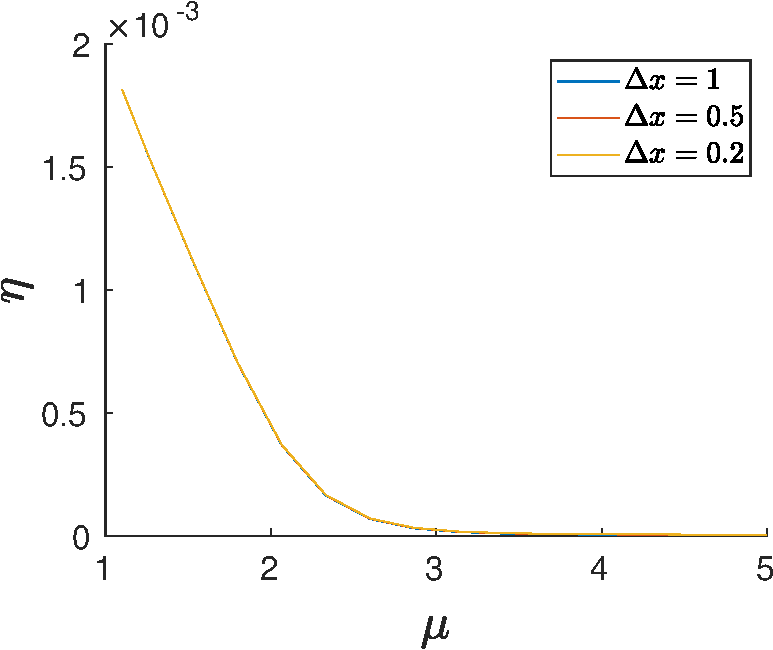
\includegraphics[width=.50\textwidth]{OneStateForager_varying-dx_PowerLaw_D_lambda1000_rv1_lmin1}\label{fig:OneStateForager_PowerLaw_D}}\hfill
	\subfloat[{Non-destructive foraging ($x_0=r_v$)}]{%
		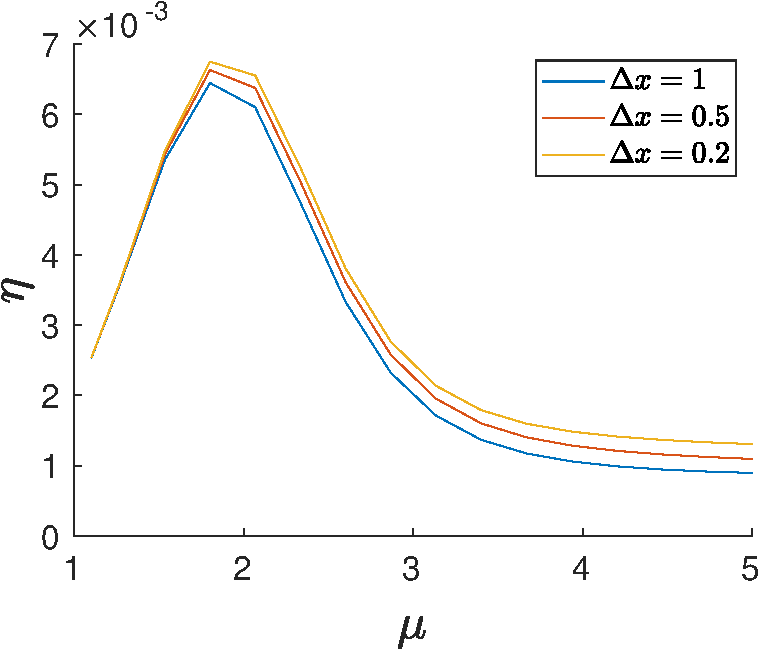
\includegraphics[width=.50\textwidth]{OneStateForager_varying-dx_PowerLaw_ND_lambda1000_rv1_lmin1}\label{fig:OneStateForager_PowerLaw_ND}}\\
	\caption[Search efficiency of an unbounded power-law strategy across a range of different discretisation sizes]{Search efficiency, $\eta$, versus distribution parameter $\mu$, of a power-law step-length distribution strategy with model parameters: $\lambda = 1000$, $r_v=1$, $\lmin = 1$, and simulations run with three different discretisation sizes, $\Delta x = \{1,0.5,0.2\}$. \label{fig:OneStateForager_PowerLaw}}
\end{figure}

\cref{fig:OneStateForager_PowerLaw_D,fig:OneStateForager_PowerLaw_ND} both match the results of Bartumeus \etal \cite{Bartumeus_2013} exactly. The optimal parameter, $\mu$, for destructive foraging with a power-law distribution is $\mu \to 1$, and for non-destructive foraging is $\mu \approx 2$, which matches the conclusions of the literature (e.g. \cite{Viswanathan_1999,Bartumeus_2013}). 

With the bounded power-law distribution, \cref{fig:OneStateForager_PowerLawBounded_D} shows that the efficiency appears to be very similar to the unbounded power-law, with the biggest difference coming as $\mu \to 1$. An explanation for this is that the closer $\mu$ to $1$, the more likely that there are steps that are large enough to be truncated. When $\mu$ is larger, especially $\mu \geq 3$, the distribution has a finite variance and the chances of taking a step larger than $\lmax = 100$ is very low. The non-destructive case is shown in \cref{fig:OneStateForager_PowerLawBounded_ND}, although the efficiency curve is approximately the same shape, there the peak efficiency is shifted slightly towards a larger $\mu$. The peak efficiency ($\eta \approx 3 \times 10^{-3}$) is also much lower than that of the unbounded power-law ($\eta \approx 7 \times 10^{-3}$). The most efficient choice of parameter is now slightly larger than $\mu = 2$, rather than slightly below $\mu = 2$ as with the unbounded distribution. The bounded power-law distribution for the non-destructive case also seems to be relatively sensitive to the discretisation size. 


\begin{figure}[h!]
	\centering
	\subfloat[{Destructive foraging ($x_0=\lambda/2$)}]{%
		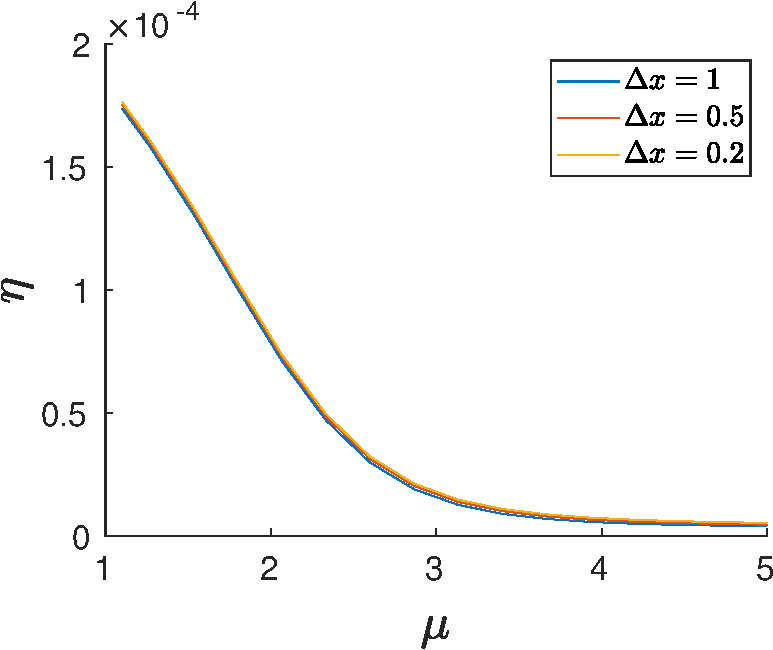
\includegraphics[width=.50\textwidth]{OneStateForager_varying-dx_PowerLawBounded_D_lambda1000_rv1_lmin1_lmax100}\label{fig:OneStateForager_PowerLawBounded_D}}\hfill
	\subfloat[{Non-destructive foraging ($x_0=r_v$)}]{%
		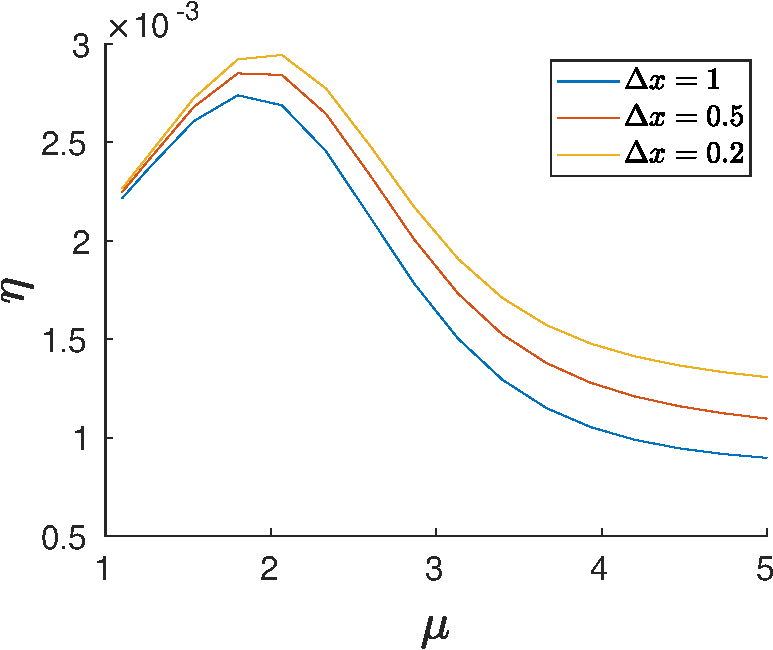
\includegraphics[width=.50\textwidth]{OneStateForager_varying-dx_PowerLawBounded_ND_lambda1000_rv1_lmin1_lmax100}\label{fig:OneStateForager_PowerLawBounded_ND}}\\
	\caption[Search efficiency of a bounded power-law strategy across a range of different discretisation sizes]{Search efficiency, $\eta$, versus distribution parameter $\mu$, of a bounded power-law step-length distribution strategy with model parameters: $\lambda = 1000$, $r_v=1$, $\lmin = 1$, $\lmax=100$, and simulations run with three different discretisation sizes, $\Delta x = \{1,0.5,0.2\}$ \label{fig:OneStateForager_PowerLawBounded}}
\end{figure}

To understand why the upper bound on the step-length distribution results in a worse efficiency, recall that for the unbounded power-law strategy, the peak efficiency was around $\mu=2$, which is a L\'{e}vy walk. This strategy would have mostly small steps, but every so often would take very large steps, allowing the forager to travel a large distance without any backtracking. However, with a small $\lmax$, the forager is unable to make these large steps,

The efficiency of the unbounded exponential strategy in \cref{fig:OneStateForager_Exponential_D} is optimal with $\mu \to 0$, and has a huge drop off immediately as $\mu$ increases. For the non-destructive search, the unbounded exponential has an optimal efficiency when $\mu \to 0$, as seen in \cref{fig:OneStateForager_Exponential_ND}. There is a large drop off in efficiency as $\mu$ increases, though not as extreme as in the destructive case. The efficiency in the non-destructive case seems to be relatively sensitive to discretisation size.


\begin{figure}[h!]
	\centering
	\subfloat[{Destructive foraging ($x_0=\lambda/2$)}]{%
		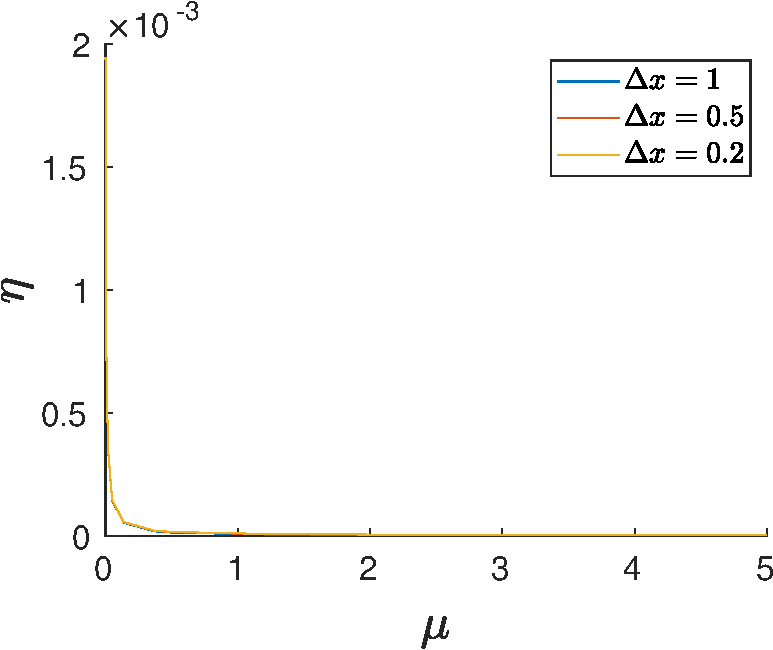
\includegraphics[width=.50\textwidth]{OneStateForager_varying-dx_Exponential_D_lambda1000_rv1_lmin1}\label{fig:OneStateForager_Exponential_D}}\hfill
	\subfloat[{Non-destructive foraging ($x_0=r_v$)}]{%
		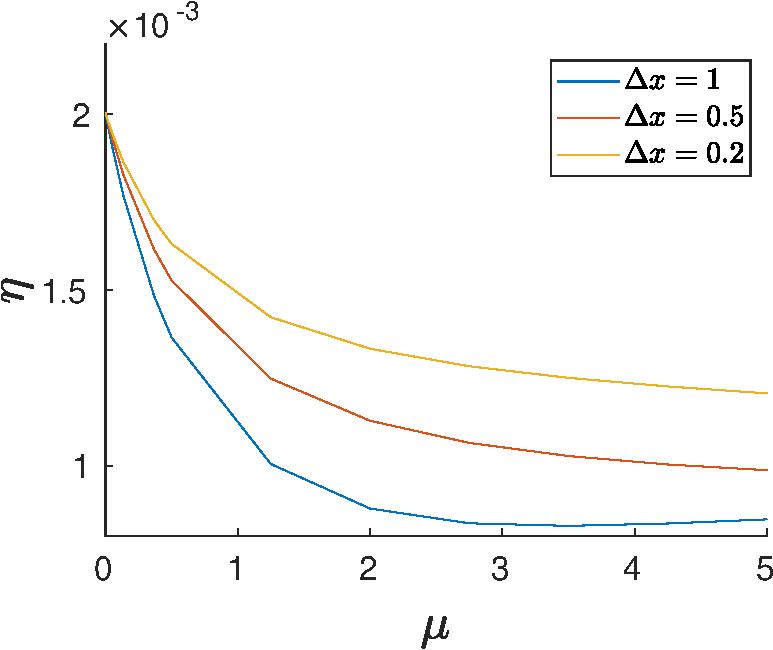
\includegraphics[width=.50\textwidth]{OneStateForager_varying-dx_Exponential_ND_lambda1000_rv1_lmin1}\label{fig:OneStateForager_Exponential_ND}}\\
	\caption[Search efficiency of an unbounded exponential strategy across a range of different discretisation sizes]{Search efficiency, $\eta$, versus distribution parameter $\mu$, of an exponential step-length distribution strategy with model parameters: $\lambda = 1000$, $r_v=1$, $\lmin = 1$, and simulations run with three different discretisation sizes, $\Delta x = \{1,0.5,0.2\}$. \label{fig:OneStateForager_Exponential}}
\end{figure}

Finally, we consider the bounded exponential in \cref{fig:OneStateForager_ExponentialBounded_D,fig:OneStateForager_ExponentialBounded_ND} for destructive and non-destructive foraging, respectively. The destructive foraging efficiency looks very similar to that of the unbounded exponential. The non-destructive foraging follows a similar pattern as the unbounded exponential distribution, although the drop off in efficiency as $\mu$ increases is not as pronounced. The optimal efficiency for both of these cases is found as $\mu \to 0$, which corresponds to the steps getting larger.


\begin{figure}[h!]
	\centering
	\subfloat[{Destructive foraging ($x_0=\lambda/2$)}]{%
		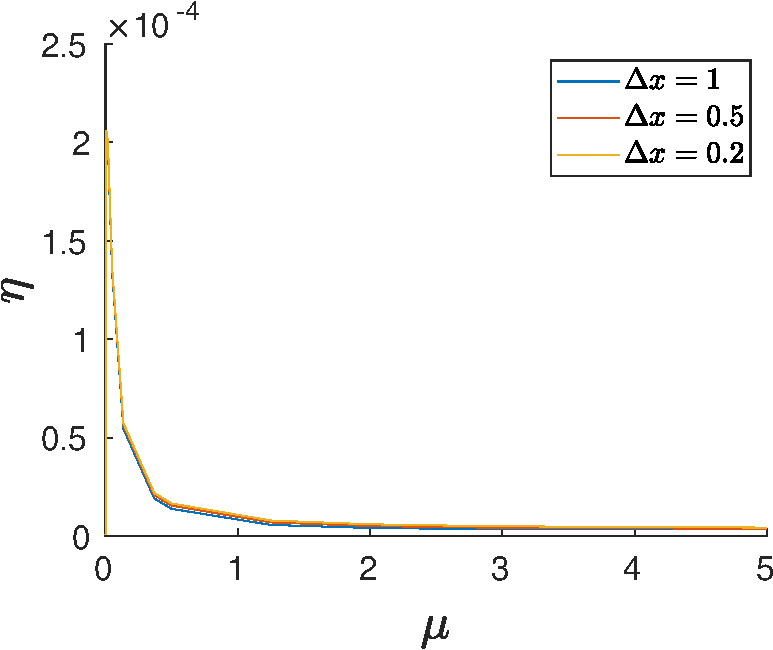
\includegraphics[width=.50\textwidth]{OneStateForager_varying-dx_ExponentialBounded_D_lambda1000_rv1_lmin1_lmax100}\label{fig:OneStateForager_ExponentialBounded_D}}\hfill
	\subfloat[{Non-destructive foraging ($x_0=r_v$)}]{%
		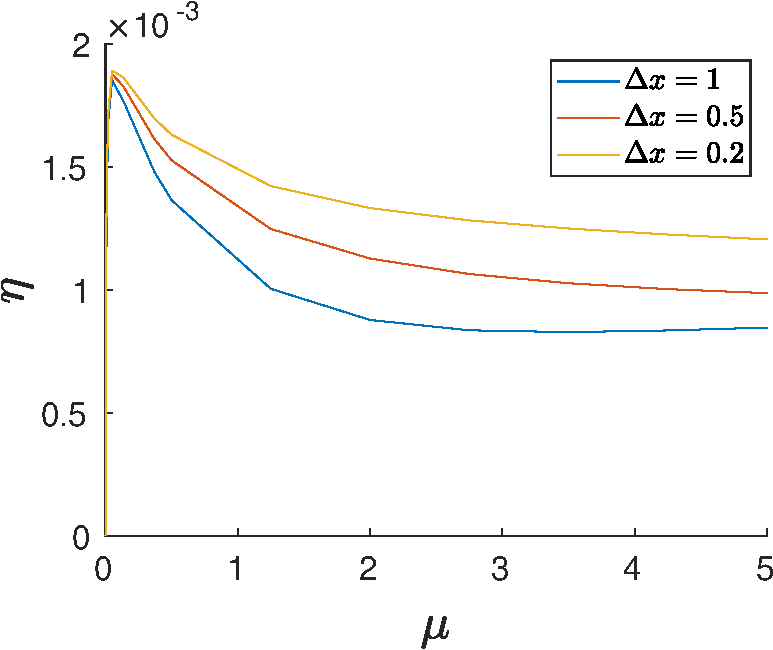
\includegraphics[width=.50\textwidth]{OneStateForager_varying-dx_ExponentialBounded_ND_lambda1000_rv1_lmin1_lmax100}\label{fig:OneStateForager_ExponentialBounded_ND}}\\
	\caption[Search efficiency of a bounded exponential strategy across a range of different discretisation sizes]{Search efficiency, $\eta$, versus distribution parameter $\mu$, of a bounded exponential step-length distribution strategy with model parameters: $\lambda = 1000$, $r_v=1$, $\lmin = 1$, $\lmax=100$, and simulations run with three different discretisation sizes, $\Delta x = \{1,0.5,0.2\}$ \label{fig:OneStateForager_ExponentialBounded}}
\end{figure}

It is worth noting that a strategy that involved simply choosing a direction at random and walking in a straight line (ballistic motion) will have an efficiency of $\eta = 2\times 10^{-3}$ for $\lambda = 10^{-3}$, since the expected distance travelled will be $\lambda/2$, regardless of starting position. Of the strategies investigated above, the only time an efficiency greater than $2 \times 10^{-3}$ was achieved was for both the bounded and unbounded power-law distributions, and only for non-destructive foraging. For the unbounded power-law distribution, if the parameter is in the approximate range $1.1 \leq \mu \leq 2.8$, then an efficiency greater than that of ballistic motion will be achieved. Similarly, for the bounded power-law distribution, although the range is slightly smaller, requiring approximately $1.1 \leq \mu \leq 2.6$.

To help summarise the results of comparing these four step-length distributions, we plot the efficiency of all four on a single plot, in \cref{fig:OneStateForager_AllDists_D} for destructive foraging and \cref{fig:OneStateForager_AllDists_ND} for non-destructive foraging. 


\begin{figure}[h!]
	\centering
	\subfloat[{Destructive foraging ($x_0=\lambda/2$)}]{%
		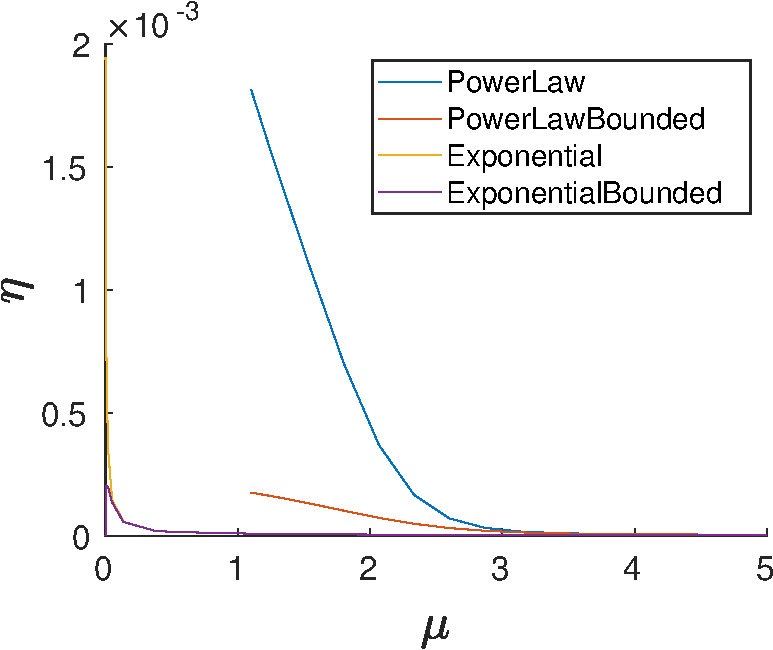
\includegraphics[width=.50\textwidth]{OneStateForager_AllDists_D_M5000_rv1_lmin1_lmax100}\label{fig:OneStateForager_AllDists_D}}\hfill
	\subfloat[{Non-destructive foraging ($x_0=r_v$)}]{%
		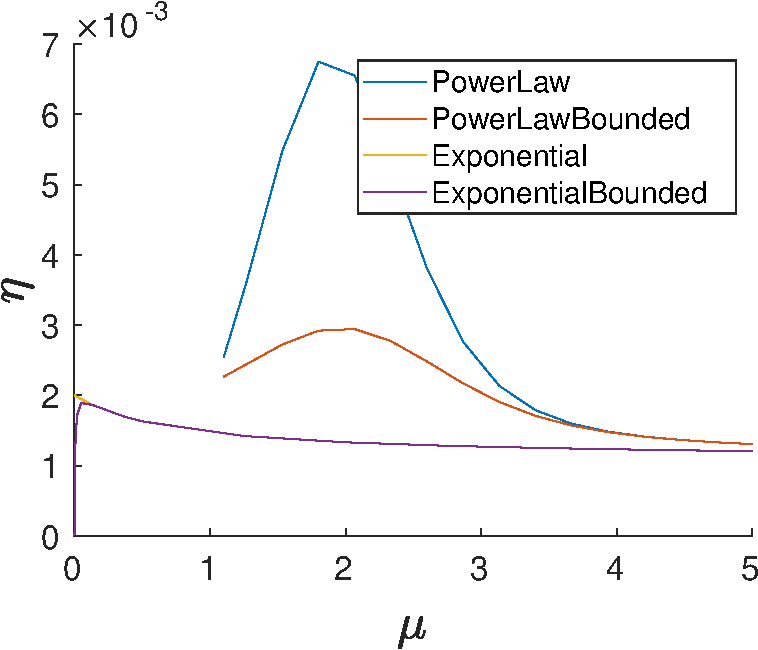
\includegraphics[width=.50\textwidth]{OneStateForager_AllDists_ND_M5000_rv1_lmin1_lmax100}\label{fig:OneStateForager_AllDists_ND}}\\
	\caption[Comparison of the search efficiency for the four different step-length distributions]{Search efficiency, $\eta$, versus distribution parameter $\mu$, for all four step-length distributions with model parameters: $\lambda = 1000$, $r_v=1$, $\lmin = 1$, $\lmax=100$, and simulations run using discretisation size $\Delta x =0.2$. \label{fig:OneStateForager_AllDists}}
\end{figure}

We also investigate the effect of the size of the upper bound, by plotting the efficiency of the bounded power-law and bounded exponential distributions for a range of $\lmax$, for both destructive and non-destructive foraging. Based on \cref{fig:EffectOfBound_PowerLawBounded_D,fig:EffectOfBound_PowerLawBounded_ND,fig:EffectOfBound_ExponentialBounded_D,fig:EffectOfBound_ExponentialBounded_ND}, the larger $\lmax$ is, the higher the efficiency of a foraging strategy, although for the exponential distribution an effect is only properly noticed for $\mu \to 0$. It is also worth noting that the graphs of the bounded distributions look the same as the corresponding unbounded distributions as $\lmax \to \infty$, which is to be expected since we recover the unbounded distributions as $\lmax \to \infty$. When $\lmax =1000$, the bounded distributions have a different distribution to the unbounded, even though a step can reach the boundary from any point, which seems counter-intuitive. This occurs because the bounded distribution is being normalised over $\lmin$ to $\lmax$, where $\lmax$ is finite, meaning larger steps are still less likely than they are for the unbounded distributions.

\begin{figure}[h!]
	\centering
	\subfloat[{Destructive foraging ($x_0=\lambda/2$)}]{%
		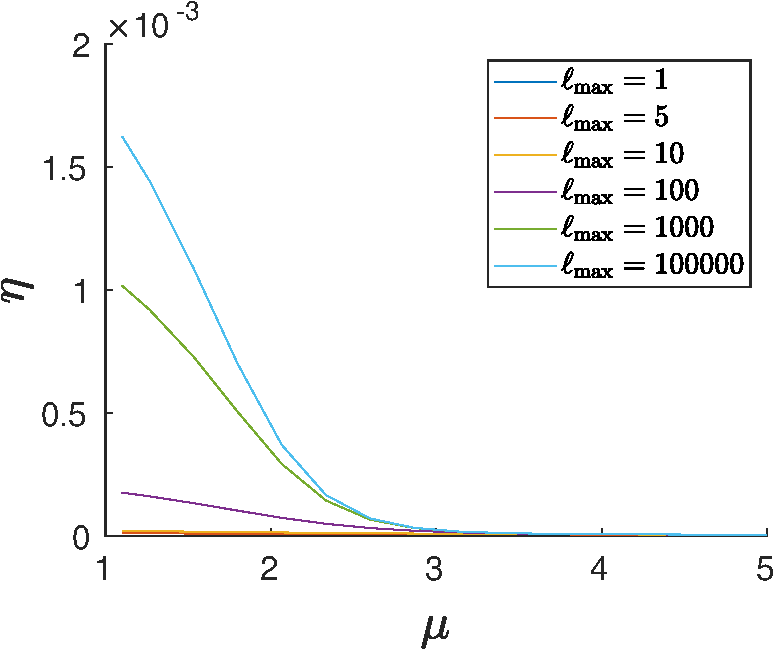
\includegraphics[width=.50\textwidth]{OneStateForager_varying-lmax_PowerLawBounded_D_M5000_rv1_lmin1}\label{fig:EffectOfBound_PowerLawBounded_D}}\hfill
	\subfloat[{Non-destructive foraging ($x_0=r_v$)}]{%
		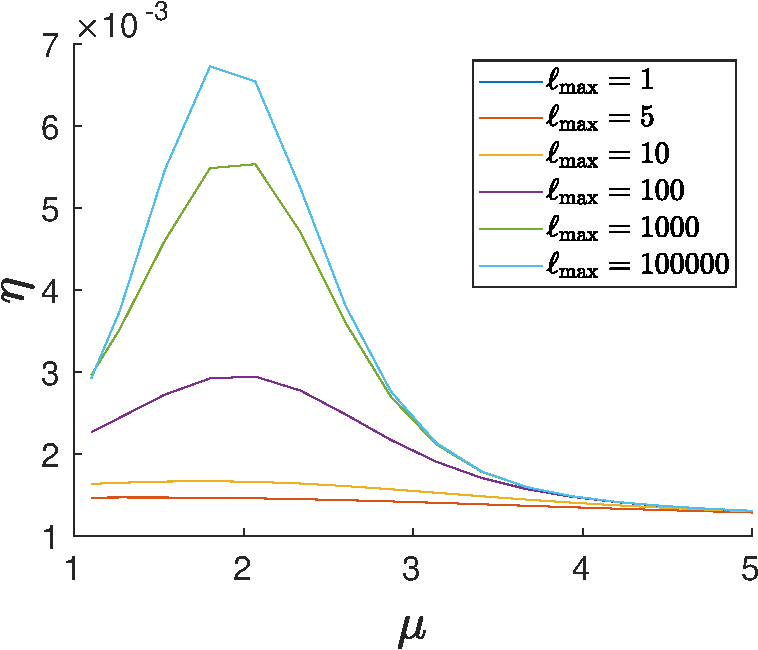
\includegraphics[width=.50\textwidth]{OneStateForager_varying-lmax_PowerLawBounded_ND_M5000_rv1_lmin1}\label{fig:EffectOfBound_PowerLawBounded_ND}}\\
	\caption[Effect of bound size on the search efficiency for a bounded power-law distribution for destructive foraging]{Search efficiency, $\eta$, versus distribution parameter $\mu$, for a bounded power-law distribution with model parameters: $\lambda = 1000$, $r_v=1$, $\lmin = 1$, $\Delta x=0.2$, and simulations run across multiple different upper bounds, $\lmax = \{1,5,10,100,1000\}$.\label{fig:EffectOfBound_PowerLawBounded}}
\end{figure}

\begin{figure}[h!]
	\centering
	\subfloat[{Destructive foraging ($x_0=\lambda/2$)}]{%
		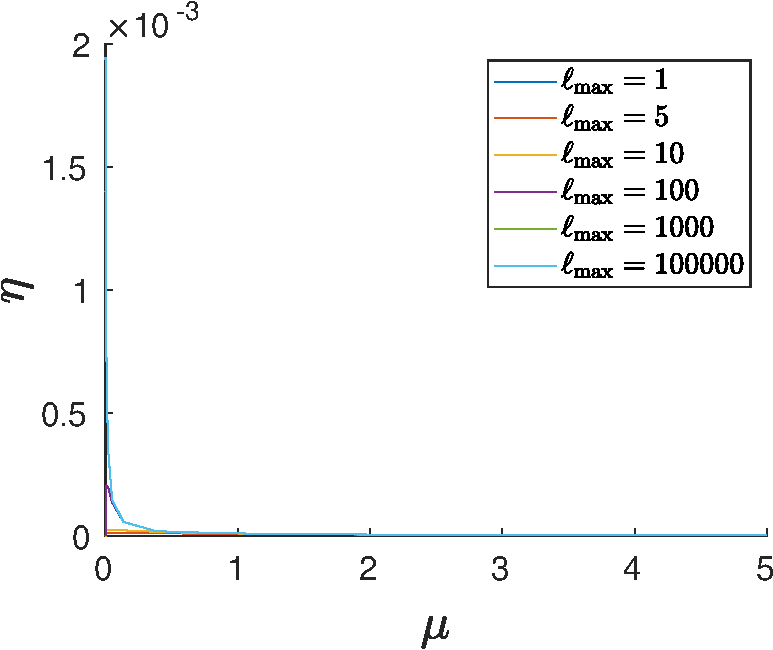
\includegraphics[width=.45\textwidth]{OneStateForager_varying-lmax_ExponentialBounded_D_M5000_rv1_lmin1}\label{fig:EffectOfBound_ExponentialBounded_D}}\hfill
	\subfloat[{Non-destructive foraging ($x_0=r_v$)}]{%
		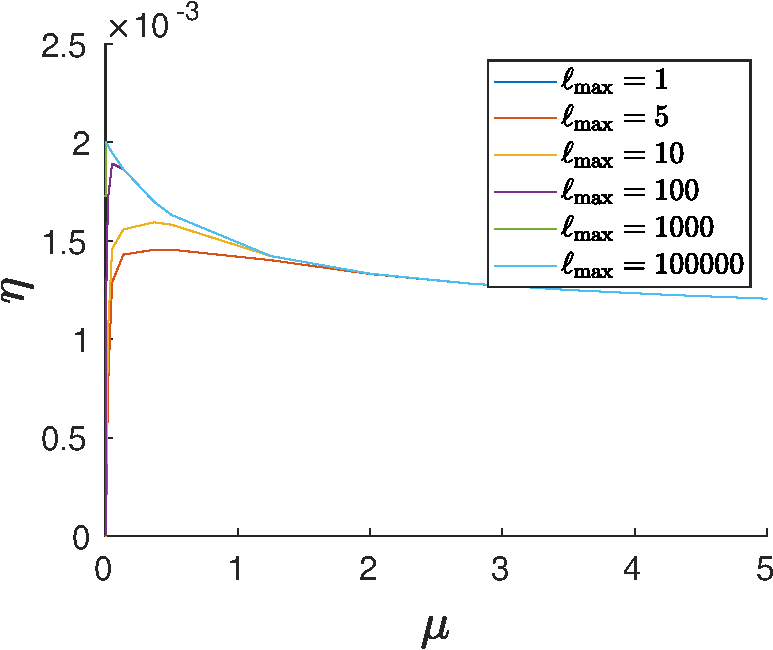
\includegraphics[width=.45\textwidth]{OneStateForager_varying-lmax_ExponentialBounded_ND_M5000_rv1_lmin1}\label{fig:EffectOfBound_ExponentialBounded_ND}}\\
	\caption[Effect of bound size on the search efficiency for a bounded exponential distribution for destructive foraging]{Search efficiency, $\eta$, versus distribution parameter $\mu$, for a bounded exponential distribution with model parameters: $\lambda = 1000$, $r_v=1$, $\lmin = 1$, $\Delta x=0.2$, and simulations run across multiple different upper bounds, $\lmax = \{1,5,10,100,1000\}$.\label{fig:EffectOfBound_ExponentialBounded}}
\end{figure}

\FloatBarrier
\subsection{Giving-up-time forager \label{sec:1dMMRW_GUT}}
Another special case of the Markov-modulated random walk is the random walk with ``giving-up time'', as discussed in papers by Benhamou \cite{Benhamou_2007}, Plank and James, \cite{Plank_2008}, and Reynolds \cite{Reynolds_2008_comment,Reynolds_2009_adaptive}.

These papers described a giving-up-time forager that undergoes an intensive search until some time, $\tau$, has elapsed, and then gives up its search and switches into an extensive search. The type of motion used in the intensive and extensive searches varies between papers, though most commonly it was Brownian motion and ballistic motion, respectively. Of the giving-up time strategies that have been investigated, the adaptive L\'{e}vy walk is the most general, which has Brownian motion for its intensive search, and the extensive search is drawn from a power-law distribution, where $\mu$ is allowed to take any value. Reynolds \cite{Reynolds_2009_adaptive} showed that his adaptive L\'{e}vy walk model could also model the previously investigated giving-up time models (e.g \cite{Plank_2008}) by setting $\mu \to 1$.

We now show that the adaptive L\'{e}vy walk can itself be thought of as a special case of a two-state Markov-modulated random walk. Furthermore, we have derived some analytic expressions for the efficiency in \cref{sec:1dMMRW_cost} and their discretised counterparts \cref{sec:1d_discrete:MMRW}, which should provide better accuracy compared to the results found by Reynolds \cite{Reynolds_2008_comment} via numerical simulation. We let state 1 represent the intensive search, and so \[p_1(x) = \frac{\mu_1-1}{\lmin}\left(\frac{\ell}{\lmin}\right)^{-\mu_1},\]
and state 2 represent the extensive search,
\[p_2(x) = \frac{\mu_2-1}{\lmin}\left(\frac{\ell}{\lmin}\right)^{-\mu_2}.\]

For a giving-up time model, the forager begins with an intensive search, and so $\vec{z_0} = (1,0)$.
When $\mu_1 \geq 3$, the intensive phase is a Brownian motion and hence we have the adaptive L\'{e}vy walk model of Reynolds \cite{Reynolds_2009_adaptive}. 
Further, when $\mu_1 \geq 3$ and $\mu_2 \to 1$, we recover the giving-up time strategy of Plank and James \cite{Plank_2008}. 
One of the earliest giving-up time strategies was the composite Brownian walk, which was introduced by Benhamou \cite{Benhamou_2007}. 
This involved exponentially distributed step-sizes for both the intensive and extensive search, though with different parameters for each. 
We may also model this using a two-state Markov-modulated random walk, by choosing exponential distributions for both states, although we do not do this since adaptive L\'{e}vy walks were found to have a better performance.

How we construct the transition matrix, $P$, will depend on how the giving-up-time, $\tau$, is defined.
For example, a geometrically distributed giving-up-time with expected value $1/p$ can be modelled with the transition matrix
\begin{equation}
\label{eq:P_geometricGUT}
P = \begin{bmatrix}
1-p & p\\
0 & 1
\end{bmatrix}.
\end{equation}
This geometric giving-up time will correspond to an exponential giving-up time in the continuous limit. If instead we have a deterministic giving-up-time, say $N$ steps before giving up, we can model this with the transition matrix
\begin{equation}
\label{eq:P_deterministicGUT}
P = \begin{bmatrix}
\vec{0}^T & \identity_N\\
0 & \vec{e}_N
\end{bmatrix},
\end{equation}
where $\vec{0} = (0,\dots,0)$ and $\vec{e}_N$ is a vector with the $N$th element a $1$ and all other elements are $0$. In this case, the first $N$ states of the Markov chain correspond to the same step-length distribution, $p_1(x)$, and the final state, state $N+1$, corresponds to the step-length distribution $p_2(x)$. 

By reordering the states of our Markov chain, we can write \cref{eq:P_geometricGUT,eq:P_deterministicGUT} in the form 
	\begin{equation*}
P = \begin{bmatrix}
1 & \vec{0} \\ 
\vec{t} & T
\end{bmatrix},
\end{equation*}
matching \cref{def:phase-type_dist}. That is, the giving-up time for both of these cases can be thought of as a discrete phase-type distribution. In fact, we can construct our states and transition matrix in such a way that we can consider any phase-type distribution for the giving-up time. Not only does this allow us to consider distributions such as geometric and negative-binomial, but using \cref{thm:PH-dense} we can approximate any possible distribution for the giving-up time using our Markov-modulated random walk.



\paragraph{Optimal giving-up time for Brownian motion giving up into ballistic motion}

Plank and James \cite{Plank_2008} described a forager that used a Brownian motion for its intensive search before giving-up into a ballistic motion for the extensive search. They were able to determine an approximate value for the optimal choice of giving-up time:
\begin{equation*}
\tau^* = \frac{d}{4v_I} \left( 1 - \frac{4}{3}\varepsilon -\frac{2}{5} \varepsilon^2 \right),
\end{equation*}
where $d$ is the distance between targets, $v_I$ is the velocity of the forager during the intensive search, and $\varepsilon = \frac{2x_0^2}{\pi v_I d} < 0.19$. If $\varepsilon > 0.19$ then the efficiency is optimised at $\tau = 0$, meaning the search is comprised entirely of ballistic motion. The average distance between patches, $d$, is equivalent to $\lambda$ in our model, and we are considering non-destructive foraging, which implies $x_0 = r_v$. Since we are considering the distance as opposed to the time required to find food, we have not yet discussed the velocity of a searcher. In the model of Plank and James \cite{Plank_2008}, a Brownian motion with variance $\sigma^2$ has velocity $v_I = \sqrt{2/\pi}\sigma$. Recalling \cref{ex:donskers}, the variance of a Brownian motion which arises as the limit of a random walk with unbounded power-law distributed steps is $\sigma^2 = (\mu-1)/(\mu-3) \lmin^2$, and we are choosing $\lmin=1$. Taking these differences into account, under our model we would expect the optimal giving-up time to be
\begin{equation*}
\tau^* = \frac{\lambda \sqrt{\pi}}{4 \sqrt{2} \sigma} \left( 1 - \frac{4}{3} \frac{2r_v^2}{\pi \lambda} - \frac{2}{5} \frac{4 r_v^4}{\pi^2 \lambda^2}\right),
\end{equation*}
with $\lambda \leq \frac{2 r_v^2}{0.19 \pi}$ implying that $\tau^* =0$. 

In our case, $\lambda = 1000$, $r_v=1$, and we choose $\mu =5$, so $\sigma = \sqrt{2}$ and $\lambda > \frac{2r_v^2}{0.19 \pi}$. Thus, the optimal giving-up time is 
\begin{equation*}
\tau^* = \frac{1000 \sqrt{\pi}}{8} \left( 1 - \frac{4}{3} \frac{2}{\pi 1000} - \frac{2}{5} \frac{4}{\pi^2 1000^2}\right) \approx 221.3686,
\end{equation*}
and so the optimal parameter $p = 1/\tau^* = 0.0045$.

We consider a Markov-modulated random walk with geometric giving-up time defined as above, with state $1$ being a power-law with $\mu =5 $, and state $2$ being a power-law with $\mu \to 1$. We use the transition matrix in \cref{eq:P_geometricGUT} and plot the efficiency of a non-destructive search for a range of different values of $p$ in \cref{fig:GeometricGUTForager_PowerLaw_ND_FixedMu}. We also use Matlab's \emph{fmincon} solver to find the optimal choice of $p$, and mark it on the plot. 

The optimal efficiency is $\eta =  0.0152$ and occurs at $p=0.0038$, which corresponds to a mean giving-up time of $263.4465$. This is not exactly the same as the value predicted by Plank and James \cite{Plank_2008}, but is a reasonable approximation, given the differences between their model and ours. Firstly, they considered a deterministic giving-up time, whereas we are considering a geometric giving-up time. We could consider a deterministic giving-up time, although to consider the values around this size, the matrix $\Amat$ would be far too large. Another difference between our model and theirs is that they considered continuous-time processes, whereas we are using discrete-time processes.

\begin{figure}[h!]
\centering
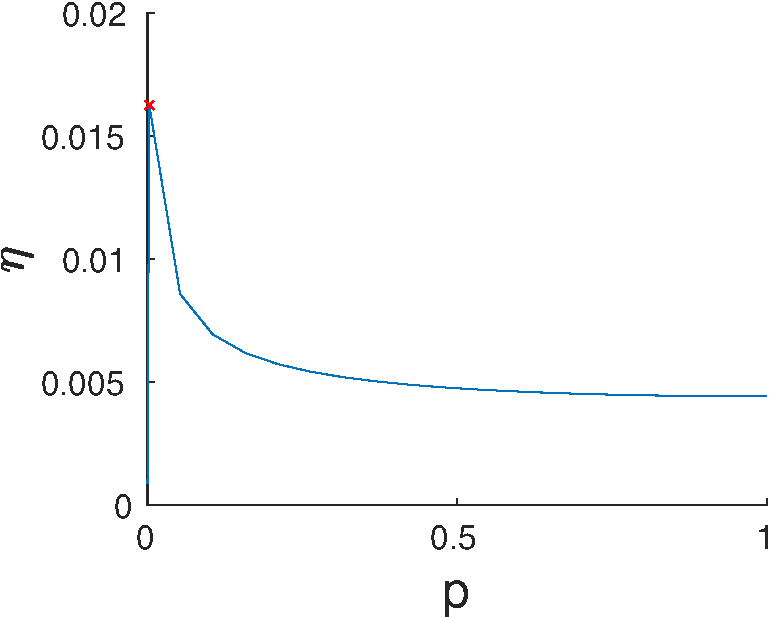
\includegraphics[scale=0.68]{GeometricGUTForager_PowerLaw_Fixedmu10-0-1-1_ND_lambda1000_rv1}
\caption[Efficiency vs geometric giving-up time parameter for a Brownian search that gives up and follows a ballistic path]{The efficiency of a non-destructive search ($x_0=r_v$) against the parameter $p$ for the geometric giving-up time. The forager uses a power-law distribution search with parameter $\mu_1 = 5$ before ``giving up'' and using a power-law search with $\mu_2 \to 1$. The peak efficiency (the red x) is $\eta = 0.0152$ which occurs at $p=0.0038$, corresponding to a mean giving-up time of $263.4465$. \label{fig:GeometricGUTForager_PowerLaw_ND_FixedMu}}
\end{figure}

\paragraph{Optimal adaptive L\'{e}vy walk parameters for fixed giving-up times}

As discussed in \cref{sec:litreview}, Reynolds \cite{Reynolds_2009_adaptive} investigated an adaptive L\'{e}vy walk, which involved switching between a power-law distribution with $\mu = 3$, and a power-law distribution with $\mu \to 1$, called the intensive and extensive phases, respectively. Reynolds also considered changing the values of $\mu$ during the extensive phase, and determined the optimal extensive search parameter. However, as correctly pointed out by Plank and James \cite{Plank_2008}, Reynolds only optimised over fixed giving-up times.

We now use our Markov-modulated random walk to investigate the adaptive L\'{e}vy walk model of Reynolds \cite{Reynolds_2009_adaptive}, although not only do we consider a range of different $\mu$ values for the extensive phase, but we also allow $\mu$ to vary in the intensive phase. We plot the efficiency at $40$ equispaced points in $1 < \mu_1 \leq 5$ and $1 < \mu_2 \leq 5$, for $5$ different choices of $p$ for a geometric giving-up time distribution.

The geometric giving-up time with the highest mean, $p=0.01$, had an optimal efficiency at $\mu_1 = 5$, and $\mu_2=1.6154$, as can be seen in \cref{fig:GeometricGUTForager_PowerLaw_ND_p0.01}. As the mean giving-up time was reduced, the optimal parameter for the intensive search does not change, but the extensive search parameter does change. For $p=0.1$ in \cref{fig:GeometricGUTForager_PowerLaw_ND_p0.1}, the optimal choice for the extensive parameter was $\mu_2= 1.7179$. For $p=0.5$, $p=0.9$, and $p=0.99$, in \cref{fig:GeometricGUTForager_PowerLaw_ND_p0.5,fig:GeometricGUTForager_PowerLaw_ND_p0.9,fig:GeometricGUTForager_PowerLaw_ND_p0.99} the optimal choice for the extensive parameter was $\mu_2=1.8205$. 

In all of these cases, the optimal extensive strategy is not a ballistic motion, but rather a L\'{e}vy flight, and the optimal intensive search is Brownian motion, matching the results of Reynolds \cite{Reynolds_2009_adaptive}. As the giving-up time increases, the extensive search gets closer to a ballistic motion, with a higher probability of very large steps, whereas for short giving-up times, the extensive parameter is closer to $\mu \approx 2$, which is the optimal for unmodulated search strategies.

In \cref{fig:GeometricGUTForager_PowerLaw_D_p0.01}, we also plot the efficiency of a giving-up time strategy for destructive foraging. Unsurprisingly, the optimal efficiency occurs at $\mu_1\to 1$ and $\mu_2 \to 1$, which is just a ballistic motion and not a true giving-up time strategy.

\begin{figure}[h!]
	\centering
	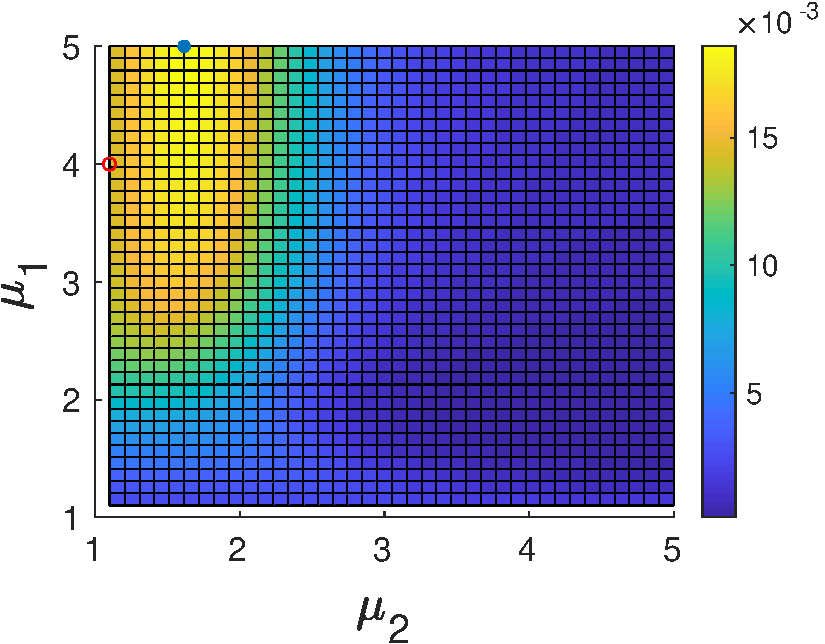
\includegraphics[scale=0.68]{GeometricGUTForager_FixedP0-01_PowerLaw_ND_lambda1000_rv1}
	\caption[Efficiency of two-state Markov-modulated power-law strategy, with giving-up parameter $p=0.01$, for non-destructive foraging]{The efficiency of a non-destructive search ($x_0=r_v$) where the forager uses a power-law distribution search with parameter $\mu_1$ before ``giving up'' and using a power-law search with $\mu_2$, after a geometrically distributed ($p=0.01$) amount of time has elapsed, which has a mean of $100$. The optimal efficiency is marked with the blue circle, and the red circle represents a Brownian motion giving-up into ballistic motion, although it is actually at any $\mu \geq 3$ rather than specifically at $\mu =4$.\label{fig:GeometricGUTForager_PowerLaw_ND_p0.01}}
\end{figure}

\begin{figure}[h!]
\centering
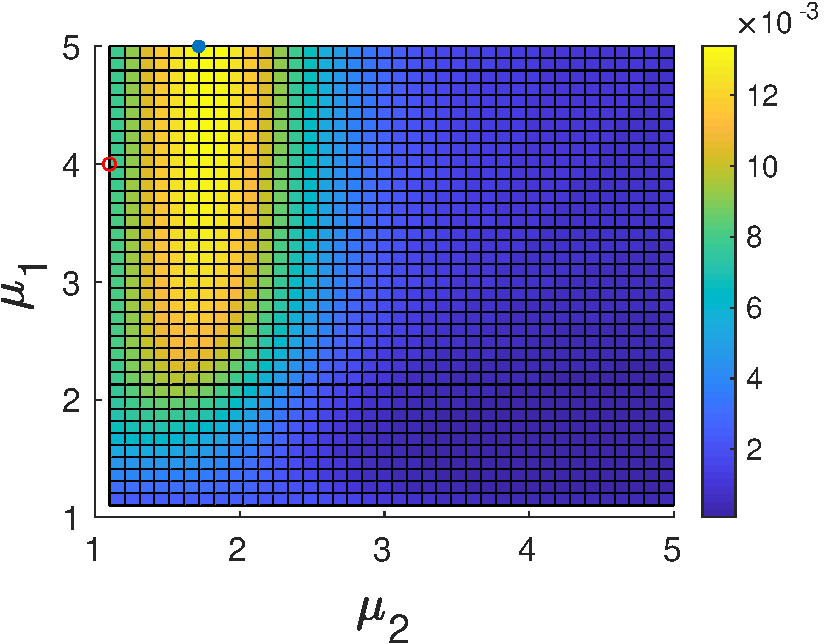
\includegraphics[scale=0.68]{GeometricGUTForager_FixedP0-10_PowerLaw_ND_lambda1000_rv1}
\caption[Efficiency of two-state Markov-modulated power-law strategy, with giving-up parameter $p=0.1$, for non-destructive foraging]{The efficiency of a non-destructive search ($x_0=r_v$) where the forager uses a power-law distribution search with parameter $\mu_1$ before ``giving up'' and using a power-law search with $\mu_2$, after a geometrically distributed ($p=0.1$) amount of time has elapsed, which has a mean of $10$. The optimal efficiency is marked with the blue circle, and the red circle represents a Brownian motion giving-up into ballistic motion, although it is actually at any $\mu \geq 3$ rather than specifically at $\mu =4$. \label{fig:GeometricGUTForager_PowerLaw_ND_p0.1}}
\end{figure}

\begin{figure}[h!]
	\centering
	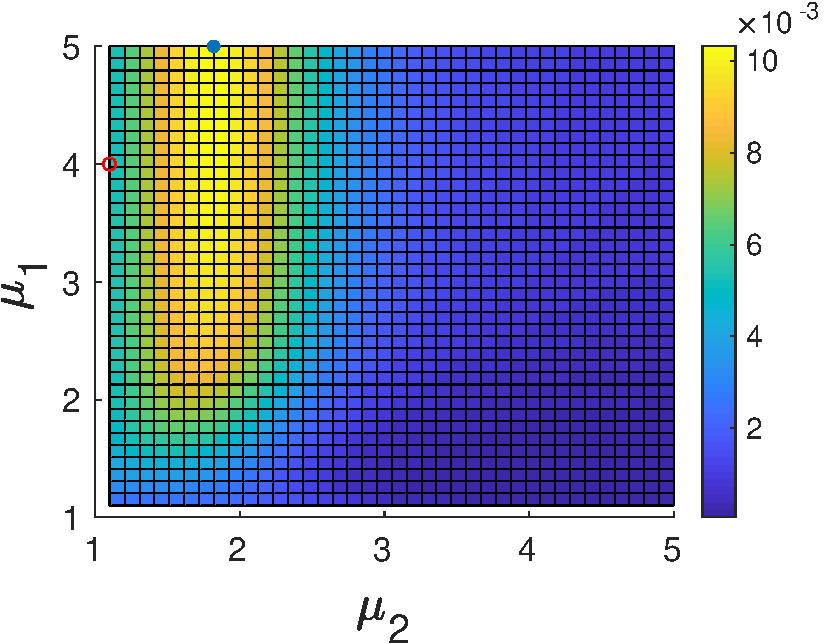
\includegraphics[scale=0.68]{GeometricGUTForager_FixedP0-50_PowerLaw_ND_lambda1000_rv1}
	\caption[Efficiency of two-state Markov-modulated power-law strategy, with giving-up parameter $p=0.5$, for non-destructive foraging]{The efficiency of a non-destructive search ($x_0=r_v$) where the forager uses a power-law distribution search with parameter $\mu_1$ before ``giving up'' and using a power-law search with $\mu_2$, after a geometrically distributed ($p=0.5$) amount of time has elapsed, which has a mean of $2$. The optimal efficiency is marked with the blue circle, and the red circle represents a Brownian motion giving-up into ballistic motion, although it is actually at any $\mu \geq 3$ rather than specifically at $\mu =4$. \label{fig:GeometricGUTForager_PowerLaw_ND_p0.5}}
\end{figure}

\begin{figure}[h!]
	\centering
	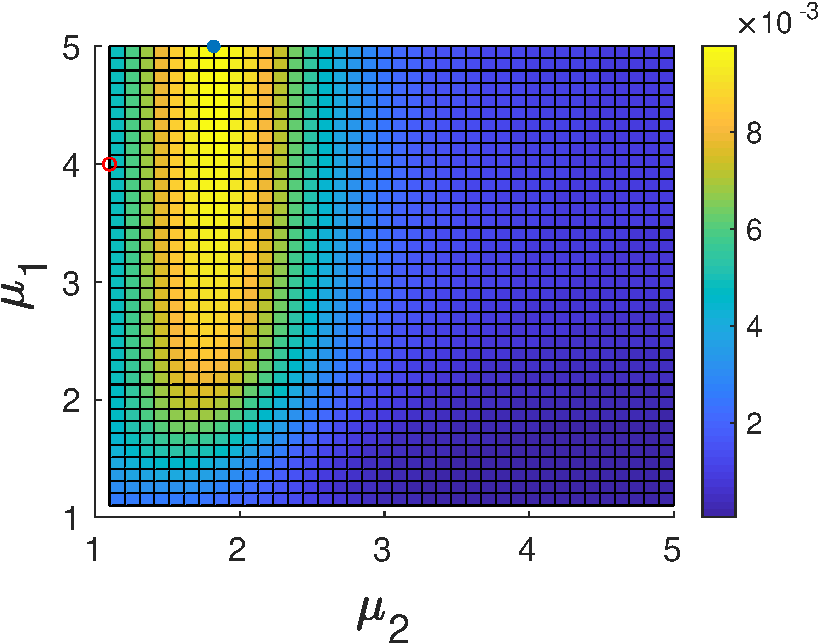
\includegraphics[scale=0.68]{GeometricGUTForager_FixedP0-90_PowerLaw_ND_lambda1000_rv1}
	\caption[Efficiency of two-state Markov-modulated power-law strategy, with giving-up parameter $p=0.9$, for non-destructive foraging]{The efficiency of a non-destructive search ($x_0=r_v$) where the forager uses a power-law distribution search with parameter $\mu_1$ before ``giving up'' and using a power-law search with $\mu_2$, after a geometrically distributed ($p=0.9$) amount of time has elapsed, which has a mean of approximately $1.11$. The optimal efficiency is marked with the blue circle, and the red circle represents a Brownian motion giving-up into ballistic motion, although it is actually at any $\mu \geq 3$ rather than specifically at $\mu =4$. \label{fig:GeometricGUTForager_PowerLaw_ND_p0.9}}
\end{figure}

\begin{figure}[h!]
	\centering
	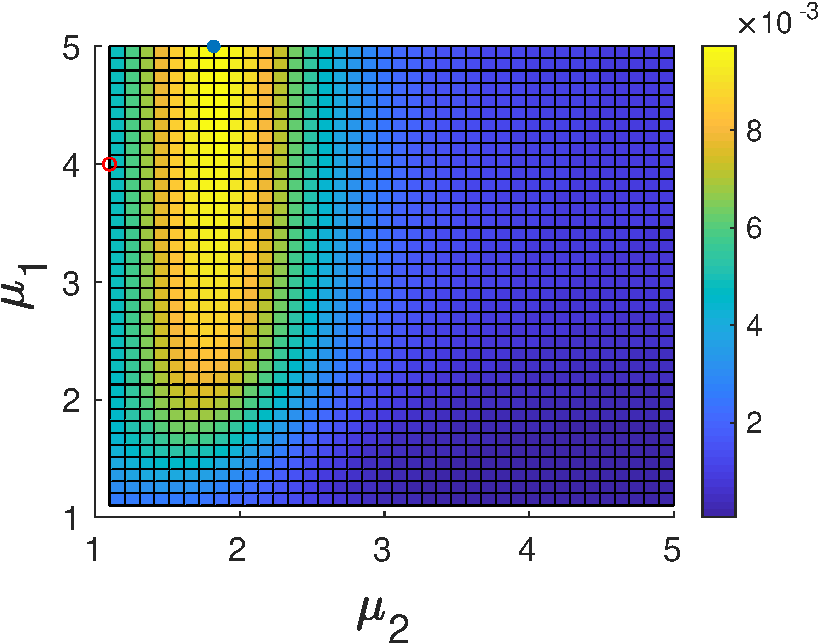
\includegraphics[scale=0.68]{GeometricGUTForager_FixedP0-99_PowerLaw_ND_lambda1000_rv1}
	\caption[Efficiency of two-state Markov-modulated power-law strategy, with giving-up parameter $p=0.99$, for non-destructive foraging]{The efficiency of a non-destructive search ($x_0=r_v$) where the forager uses a power-law distribution search with parameter $\mu_1$ before ``giving up'' and using a power-law search with $\mu_2$, after a geometrically distributed ($p=0.99$) amount of time has elapsed, which has a mean of $1.010101$. The optimal efficiency is marked with the blue circle, and the red circle represents a Brownian motion giving-up into ballistic motion, although it is actually at any $\mu \geq 3$ rather than specifically at $\mu =4$. \label{fig:GeometricGUTForager_PowerLaw_ND_p0.99}}
\end{figure}

\begin{figure}[h!]
	\centering
	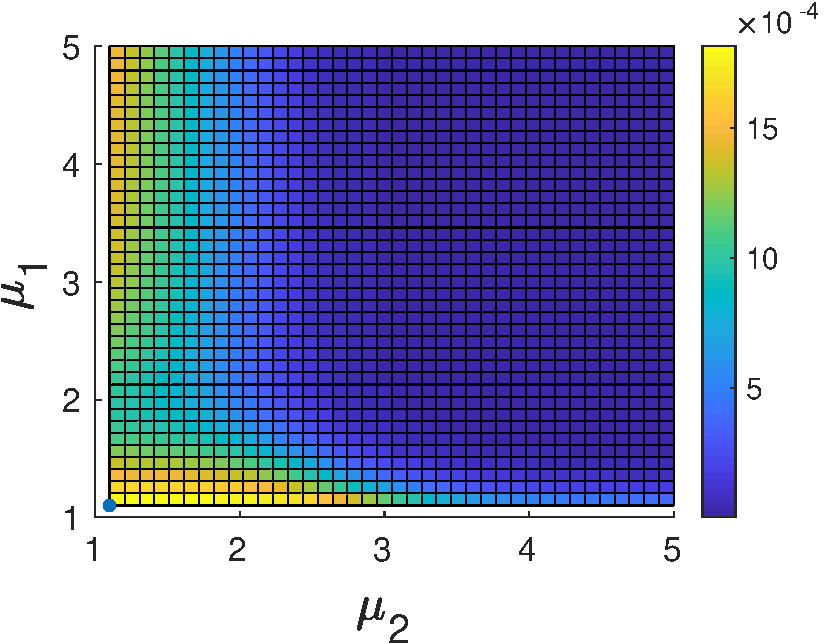
\includegraphics[scale=0.68]{GeometricGUTForager_FixedP0-01_PowerLaw_D_lambda1000_rv1}
	\caption[Efficiency of two-state Markov-modulated power-law strategy, with giving-up parameter $p=0.01$, for destructive foraging]{The efficiency of a destructive search ($x_0=\lambda/2$) where the forager uses a power-law distribution search with parameter $\mu_1$ before ``giving up'' and using a power-law search with $\mu_2$, after a geometrically distributed ($p=0.01$) amount of time has elapsed, which has a mean of $100$. The optimal efficiency is marked with the blue circle.\label{fig:GeometricGUTForager_PowerLaw_D_p0.01}}
\end{figure}

\FloatBarrier

\paragraph{Optimal geometric giving-up time strategy}

In the previous two parts, we considered the giving-up time models of Plank and James \cite{Plank_2008} and Reynolds \cite{Reynolds_2009_adaptive}. However, both of these have advantages and disadvantages. Plank and James \cite{Plank_2008} were able to find the optimal giving-up time, but considered only Brownian motion giving-up into ballistic motion. On the other hand, Reynolds \cite{Reynolds_2009_adaptive} found the optimal extensive parameters, but considered only fixed giving-up times. As shown above, we were able to use our Markov-modulated random walk strategy to investigate both of these models. Now, we can combine these ideas and use our model to optimise over both the giving-up time and the parameters $\mu_1$ and $\mu_2$.

We make use of Matlab's \emph{fmincon} function to minimise the expected total travel length, and hence maximise the efficiency over the three different parameters. We use the constraints that $0 \leq p \leq 1$, $1 < \mu_1 \leq 10$ and $1 < \mu_2 \leq 10$. 

For a non-destructive search, \emph{fmincon} finds the optimal efficiency at $p=0.0060$, $\mu_1 = 10.0000$, and $\mu_2 = 1.5868$. This value of $p$ corresponds to a mean giving-up time of approximately $167$, and the optimal values of $\mu$ correspond to a Brownian motion for the intensive search that gives up into a L\'{e}vy walk for the extensive search. The optimal value of $\mu_1 = 10$ was the maximum allowed value of $\mu_1$ according to our constraints. Increasing this upper bound will change the optimal value of $\mu_1$ accordingly, although it only changes the efficiency very slightly.

\subsection{Vision switching forager \label{sec:1dMMRW_VisionSwitching}}
Benichou \etal \cite{Benichou_2005} defined a model where the forager switches between two states an unlimited number of times. The time spent in each of the states is exponential. However, while in one of the two states, the forager cannot locate any targets.

Although this scenario cannot be modelled directly with our model, we can model a scenario which should produce very similar results. In the model outlined by Benichou \etal \cite{Benichou_2005}, when the forager is unable to locate targets, reaching a food target is impossible. However, in our model, even when the radius of vision is $0$, it is still possible for a forager to locate a target by running into it, or jumping beyond it and being truncated. To alleviate this issue, we could define the distance between food patches to be very large, and then have the radius of vision switch between a very large value and zero. However, in practice this is not feasible since a L\'{e}vy walk has heavy-tailed steps and so there is no choice of distance between targets that is sufficiently large.

For example, say we wanted to investigate food patches that are a distance $\lambda$ apart, and have the animal unable to locate a food patch during one of the two search modes, and have a radius of vision, $r_v$, during the other mode. Then, we can model this approximately using an interval size of $\lambda^*$, with $\lambda^* \gg \lambda$, and choosing $r_1 = r_v + (\lambda^* - \lambda)$ and $r_2 = 0$. Then, as long as $\lambda^*$ is sufficiently large the animal will never locate a patch while in state $2$, and while in state $1$ the scenario is equivalent to a search with food at the endpoints of $[r_v,\lambda-r_v]$. The downside to this approximation is that the size of the matrix that must be solved will be very large when $\lambda^*$ is very large, although the increase with $\lambda^*$ is only linear. Also, we could only realistically investigate search strategies that are not heavy-tailed.

Although we cannot easily investigate hidden targets with our Markov-modulated random walk model, we can consider some difficult-to-detect targets and models where adjustments to the forager's radius of vision occur. A difficult-to-detect target may be harder to find in a certain mode, but it does not necessarily have to be impossible to find targets in this mode. Thus, we can define $\lambda^*$, $\lambda$, $r_1$ and $r_2$ as above, although we no longer required $\lambda^*$ to be large enough to prevent a certain step from reaching this boundary. Other models that involve a change in the forager's radius of vision are easily modelled using our Markov-modulated random walk. A model like this may occur in nature, for example, when the weather changes from sunny to foggy, resulting in a degradation of a forager's perceptive ability. 

One possible way to extend our Markov-modulated random walk to allow us to investigate hidden and hard-to-detect targets is by defining some kind of periodic boundary conditions on the interval $[0,\lambda]$. Making this extension will be fairly involved, and is not something we do in this thesis, though we discuss some further details in \cref{sec:conclusion}. 

We now consider two different strategies for non-destructive searching, on a search space of length $\lambda=1000$. We plot the efficiency of a two-state power-law strategy against the parameters of $\mu$ in \cref{fig:visionswitching}, where the Markov chain is given by
\begin{equation*}
P = \begin{bmatrix}
0.5 & 0.5\\
0.5 & 0.5
\end{bmatrix},
\end{equation*} and $\vec{z_{0}} = (0.5,0.5)$. In \cref{fig:visionswitching_base}, we plot the efficiency of a strategy with $r_v=50$ in both states, and in \cref{fig:visionswitching_switch}, we plot the efficiency of a strategy that switches between $r_v=50$ and $r_v=0$.
\begin{figure}[h!]
	\centering
	\subfloat[{$r_v=50$ for both states}]{%
		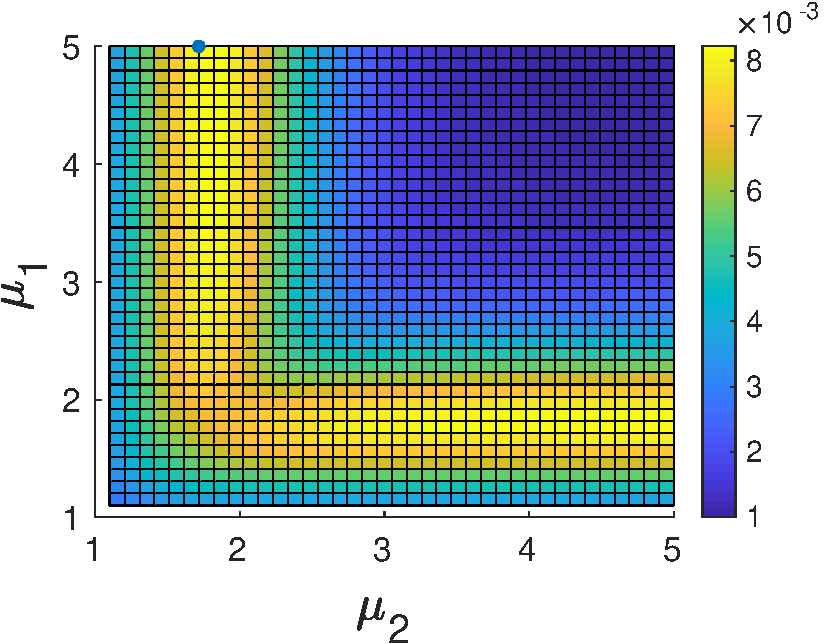
\includegraphics[width=.50\textwidth]{VisionSwitchingForager_J2_PowerLaw_ND_lambda1000_rv50-50}\label{fig:visionswitching_base}}\hfill
	\subfloat[{Switching between $r_v=50$ and $r_v=0$.}]{%
		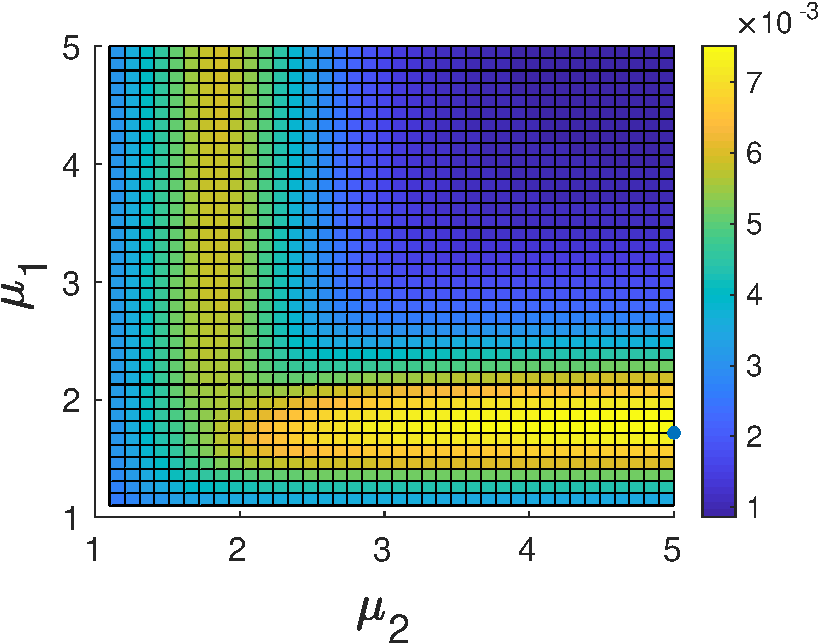
\includegraphics[width=.50\textwidth]{VisionSwitchingForager_J2_PowerLaw_ND_lambda1000_rv50-0}\label{fig:visionswitching_switch}}\\
	\caption[Efficiency of two-state Markov-modulated power-law strategy, with switching radius of vision]{The efficiency of a non-destructive search ($x_0=50$) where the forager switches between two power-law distributions with parameters $\mu_1$ and $\mu_2$, with equal probability of switching between states. The radius of vision is different for each subplot. The optimal efficiency is marked with a blue circle.}\label{fig:visionswitching}
\end{figure}
One important thing to note about \cref{fig:visionswitching_switch} is that the efficiency is not longer symmetric about the $\mu_1=\mu_2$ line, as it is for \cref{fig:visionswitching_base}. For both scenarios, large efficiencies occur for strategies that switch between a Brownian motion and a L\'{e}vy walk, though for the vision switching strategy the efficiency is much worse, as expected, if the Brownian motion occurs in state $1$ while the vision is low. 
\section{Optimal Markov-modulated search strategies for two-states, three states, and higher}
\label{sec:1dMMRW_all}
In \cref{sec:1dMMRW_GUT}, we used Markov-modulated random walk strategies to consider a giving-up time forager. These giving-up time strategies are a special case of Markov-modulated random walks in which there is an absorbing state. In this section, we consider more general Markov-modulated random walk strategies that do not necessarily have an absorbing state. For a strategy with two states, the Markov chain will have a transition matrix
\begin{equation}
\label{eq:1dresults:2state}
P = \begin{bmatrix}
1-a & a\\
b & 1-b
\end{bmatrix},
\end{equation}
where $a, b \in [0,1]$. For three states, the transition matrix is
\begin{equation*}
P = \begin{bmatrix}
1-a-b & a & b\\
c & 1-c -d & d\\
e & f & 1-e-f
\end{bmatrix},
\end{equation*}
where $a,b,c,d,e,f \in [0,1]$. 
We can continue in this manner, defining the transition matrix for higher-state Markov-modulated random walk strategies. 
A $J$-state Markov-modulated random walk will have $J^2-J$ free variables in its transition matrix.
For a $J$-state Markov-modulated random walk, we also have $J$ different step-length distributions. We choose these step-length distributions to all be unbounded power-law distributions, since they offered the highest efficiency in previous sections, although there is nothing preventing us from considering any other combination of distributions. Each step-length distribution may have a different parameter $\mu$, and we choose $\lmin = 1$ and $r_v=1$ for all distributions, for simplicity. Finally, the initial distribution of the Markov chain has $J-1$ parameters, since it must sum to one. Thus, we have $J$ different parameters for the distributions, $J^2-J$ for the transition matrix, and $J-1$ for the initial distribution, totalling $J^2+J-1$ parameters. The evaluation of the efficiency for any set of parameters also becomes slower for larger $J$, since the matrix $\Amat$ has dimensions $J(M-1)\times J(M-1)$. Because of this, we only consider search strategies with up to $J=3$ states.

We once again use Matlab's \emph{fmincon} to minimise the expected total travel length and hence maximise the efficiency. We begin with a strategy where $J=1$ with an initial guess of $\mu=2$. As we increase the number of states to $J$, we use the optimal solution for $J-1$ states to determine an initial guess for \emph{fmincon}. The transition matrix gets an extra column, with each element being $1/J$. To compensate and ensure the row sums equal $1$, the transition matrix elements from the previous solution are all scaled by $(J-1)/J$ so they sum to $1-(1/J)$ rather than $1$. We also add an extra row to the bottom of the previous transition matrix, with each element being $1/J$. For example, if the optimal solution for the $J=2$ strategy was given by \cref{eq:1dresults:2state}, then the initial guess for the $J=3$ strategy is
\begin{equation*}
P = \begin{bmatrix}
2(1-a)/3 & 2a/3 & 1/3\\
2b/3 & 2(1-b)/3 & 1/3\\
1/3 & 1/3 & 1/3
\end{bmatrix}.
\end{equation*}
Our initial guess for the new parameter $\mu$ is the mean of the other $\mu$ values. For the $J$ strategy, our initial guess for the initial distribution, we take the optimal choice for the $J-1$ strategy and add an element $1/J$ for the final state, and renormalise the other states by multiplying them by $(J-1)/J$. For example, if the $J=2$ had an optimal initial distribution of
\begin{equation*}
\vec{z_{0}} = (a,1-a),
\end{equation*}
with $a \in [0,1]$, then our initial guess for the initial distribution is
\begin{equation*}
\vec{z_0} = \left(2a/3, 2(1-a)/3, 1/3 \right).
\end{equation*}

\paragraph{Results of \emph{fmincon}}
For the $1$-state forager, the optimal strategy is $P=[1]$, $\vec{z_{0}}=[1]$, and $\mu = 1.8699$. This is a L\'{e}vy walk, matching the results we found in \cref{sec:1dMMRW_nonMM},

For the $2$-state forager, the optimal strategy is a transition matrix given by
\begin{equation*}
P = \begin{bmatrix}
0.9940  &  0.0060\\
0  &  1
\end{bmatrix},
\end{equation*}
an initial probability vector $\vec{z_{0}} = (1, 0)$ and distribution parameters $\vec{\mu} = (10,    1.5868)$. This result is interesting, since the optimal general $2$-state strategy is, in fact, a giving-up time strategy, with the same parameters as found in \cref{sec:1dMMRW_GUT}. This corresponds to a forager that begins using Brownian motion, before giving up after a geometrically distributed amount of time with an approximate mean of $166.66$ steps, before performing a L\'{e}vy flight with $\mu=1.5868$. 

For the $3$-state forager, the optimal strategy is a transition matrix given by
\begin{equation*}
P = \begin{bmatrix}
 0.9849  &  0 &   0.0151\\
0  &  1  &  0\\
0 &  0.0152   & 0.9848
\end{bmatrix},
\end{equation*}
an initial probability vector $\vec{z_{0}} = (1,0,0)$, and distribution parameters $\vec{\mu} = (10, 1.3908,    2.4368)$. This strategy once again corresponds to a giving-up time strategy that begins following a Brownian motion, before giving-up into a L\'{e}vy flight, with parameter $\mu = 2.4368$. Then, after some further time, the forager gives up again, and switches to a L\'{e}vy flight with $\mu = 1.3908$, which will somewhat resemble a ballistic path, due to the small $\mu$ parameter. The mean of both geometrically distributed giving-up time are approximately $66$ steps.
\end{chapter}

% Chapter 6: Two-dimensional models
\begin{chapter}{Two-dimensional Foraging Models\label{sec:2dmodel}}
%!TEX root = ../thesis.tex
\section{General assumptions}

We consider a forager in two dimensions, searching for targets that are scattered throughout a boundaryless search space $\mathbb{R}^2$.
Targets are represented by points that are randomly distributed in the search space according to a homogeneous spatial Poisson point process.

We only consider destructive foraging in this \lcnamecref{sec:2dmodel}, since non-destructive foraging is more complicated.
%We discuss how non-destructive foraging may be investigated using this model in \cref{sec:conclusions}.
We discuss how non-destructive foraging may be investigated using this model in Chapter 7.

The forager begins its search at some point which we define to be the origin.
Each step in the forager's search strategy involves two parts.
Firstly, the forager selects a search direction, $\theta_i$, measured in radians about a unit circle centred at the current location.
Secondly, the forager selects a step length, $\ell_i$, in which to travel in the chosen direction. We can also define the \emph{turning angle}, $\beta_i:=\theta_i-\theta_{i-1}$, which is the change in direction from the previous step's direction, measured in radians.
The location of a forager after taking $i$ steps is then denoted as $(x_i,y_i)$.
The forager also has a constant radius of vision, $r_v$, and whenever a target is within this range the forager will be able to detect it and move directly towards it.
As a forager takes a step it can still detect targets while moving, and so each step will have an area of vision associated with it.

The possible search strategies that we consider are random walks with any choice of step-length distribution, and with uniform turning angles. 
Some extensions to the model are possible, such as allowing for arbitrary distributions for the turning angle, as well as considering Markov-modulated random walks, or even non-destructive targets,   although these may make the model intractable. 
We discuss some of these further in \cref{sec:conclusion}.

We begin by making a simplifying assumption: upon revisiting a previously explored area, a forager may still find targets within this area.
This is an equivalent scenario to the spatial Poisson process being redrawn in an already explored area, after a forager has already found it to be empty.
Under the simplest model, which we call the \emph{zeroth-order} approximation, the targets may have respawned in an area immediately following a search through that area.
Thus, a search that involved a lot of backtracking over the same area is not penalised for repeated searching of the same area.
In the \emph{first-order} approximation, the area covered in the previous step may not have food in it, although all area that was explored two or more steps ago may now have food. 
This means that the points within an explored area are redrawn, although with one step of lag.
This corresponds to some penalisation of backtracking, although not fully.

In general, the \emph{$n$th order} approximation means that a forager may not find food in any area already covered in the previous $n$ steps.
In the next section we solve the model analytically for both the zeroth-order and first-order models, and show why second-order and higher models are too complicated to consider analytically.
In \cref{sec:2dmodel:simulation}, we use simulations to model the same scenario, and can deduce the difference in results between different order approximations, including the case of no approximation ($\infty$-order).

As with the one-dimensional model, in two dimensions our primary aim is to determine the most efficient search strategy.
We maintain the same notion of efficiency as in the one-dimensional case. That is, the efficiency is defined as
\begin{equation}
\label{eq:2d:efficiency}
\eta = \frac{1}{\E{L}} ,
\end{equation}
where $L$ is the total distance travelled to find a target.
Based on the assumptions of our model we are able to show that this definition of efficiency is equivalent under the zeroth-order model to the efficiency as defined by Viswanathan \etal \cite{Viswanathan_1999}, which is
\begin{equation}
\label{eq:2d:vis_efficiency}
\eta = \frac{1}{\E{\abs{\ell}} \E{N}},
\end{equation}
where $\E{\abs{\ell}}$ is the expected distance travelled in a single step, and $\E{N}$ is the expected number of steps to find a target.

Due to the complete spatial randomness of the target distribution, we can make a few simplifications to the model.
The probability of a target being within some searched area depends on the size of the area and the density of the targets.
Since the targets have a homogeneous spatial Poisson distribution, the density is constant everywhere.
This means that the start and end locations of a step make no difference to the probability of finding food, and what really matters is the search area covered by a step.
Thus, we do not actually need to keep track of the forager's location, and can without loss of generality assume that each step begins at the origin.
For the first-order approximation, we do need to track the search area of the previous step and determine the overlapping area between that and the current step.

We make one final assumption; that there are no targets within the initial radius of vision of the forager before taking any steps.
This is reasonable since if there was, a forager would immediately move to this food target and then begin searching again, repeating this process until there was no target within its initial radius of vision.

\iffalse
\begin{figure}
	\begin{center}
		\begin{tikzpicture}
		\filldraw[black] (0,0) circle (2pt) node[anchor=north west] {$(x_i,y_i)$};
		
		\draw[black] (-2,2) circle (1);
		\filldraw[black] (-2,2) circle (2pt); 
		\draw[black](-2,2) -- (-1,2) node[anchor=north east] {$r_v$};
		
		\draw[black] (3,-1) circle (1);
		\filldraw[black] (3,-1) circle (2pt); 
		\draw[black](3,-1) -- (4,-1) node[anchor=north east] {$r_v$};
		
		\draw[black] (3.5,3) circle (1);
		\filldraw[black] (3.5,3) circle (2pt); 
		\draw[black](3.5,3) -- (4.5,3) node[anchor=north east] {$r_v$};
		\end{tikzpicture}
		\caption{Example layout for two-dimensional search model. targets are represented by points, and are spread out about the search space. The forager's radius of vision is represented by the circles around the targets, within which the forager can locate the food.  \label{fig:2dtargets}}
	\end{center}
\end{figure}
\fi



\section{Solving the model analytically}

In deriving an analytic expression for the efficiency, much of the process depends on the order of model we are considering. We initially begin deriving expressions for the probability of finding a target on any given step, and for the expected length of a single step, for any order of model. Then, in \cref{sec:2dmodel:0thorder} we use these expressions to find an analytic expression for the efficiency for the zeroth-order model. In \cref{sec:2d:1storder}, we consider the first-order model, and are unable to derive an exact expression for the efficiency, and we discuss why this is the case.

In \cref{sec:1dRW} we found an expression for the total cost to find a single target, which we simplified in \cref{eq:1dRW_cost:Q_rearranged} to
\begin{equation*}
Q(x_0) = \sum_{n=0}^{\infty} \indic_{(\tau \geq n+1)} q(X_n,X_{n+1}),
\end{equation*}
where $Q(x_0)$ was the total cost for a search beginning at $x_0$, and $q(X_n,X_{n+1})$ was the cost attributed to a step that begins at $X_n$ and ends at $X_{n+1}$, and the random variable $\tau$ represented the time until food was found. In the case of our two-dimensional model, we are not interested in finding a general cost function, but rather, the total length travelled to find food. Thus, we get
\begin{equation*}
L = \sum_{n=0}^\infty \indic_{(\tau \geq n+1)} \abs{\ell (X_n,X_{n+1})},
\end{equation*}
where we can also drop the dependence on the starting location $x_0$, since all starting locations are considered equivalent. 
\begin{equation*}
\E{L} = \sum_{n=0}^\infty \E{ \indic_{(\tau \geq n+1)} \abs{\ell_n (X_n,X_{n+1})}},
\end{equation*}
which we can rewrite as
\begin{equation*}
\E{L} = \sum_{n=0}^\infty \E{ \abs{\ell (X_n,X_{n+1})} \mid \indic_{(\tau \geq n+1)}} \Pr(\tau \geq n+1).
\end{equation*}
Since our step-length distribution has no dependence on the start or end locations, we may rewrite this without the dependence on $X_n$ and $X_{n+1}$. However, we include a subscript on the $\ell$ to denote the step number, since for first-order and higher models we need to keep the step number in mind. 
Thus,
\begin{equation*}
\E{L} = \sum_{n=1}^\infty \E{ \abs{\ell_n } } \Pr(\tau \geq n).
\end{equation*}
where we have also shifted the summation. 
Thus, we now have two expressions --- the expected length of a single step, and the probability that food is located within $n$ steps --- that must be found in order to solve for the efficiency. 

Both of these expressions will depend on whether we are considering the zeroth-order or the first-order approximation. Since the targets have a homogeneous spatial Poisson distribution, the starting point of a step will not affect the probability that food is located. The probability of finding exactly $k$ points within productive area $a$, with food density $\rho$, is
\begin{equation*}
\Pr(k,\rho,a) = \frac{(a\rho)^k e^{-(a\rho)}}{k!}.
\end{equation*}
Let $f_A(a)$ represent the \ac{PDF} of the area covered in a single step. The probability of not finding a target on a given step is then
\begin{align}
\Pr(\text{not found}) &= \int_{A_{\min}}^\infty \Pr \left( \text{not found} \mid A=a\right) f_A(a)da \nonumber \\ 
&=\int_{A_{\min}}^\infty\Pr(0,\rho,a)f_A(a)da \nonumber \\
&=\int_{A_{\min}}^\infty e^{-a\rho} f_A(a)da. \label{eq:2d_prob_not_found}
\end{align}
Therefore, the probability of finding a target on any given step is
\begin{equation}
\label{eq:2d_prob_found}
\Pr(\text{found}) = 1 - \int_{A_{\min}}^\infty e^{-a\rho} f_A(a)da.
\end{equation}
We use \cref{eq:2d_prob_found} to solve for $\E{N}$, although how we now proceed depends on which order of the model we are considering. We derive $\E{N}$ for the zeroth-order model in \cref{sec:2dmodel:0thorder}.

Next, we derive an expression for the expected length of a single step that is valid for any order of model. This expression is similar to the expectation of the step-length distribution, except we must take into account the possibility of a step being truncated:
\begin{equation}
\label{eq:2d_El}
\E{\abs{\ell}} = \int_{\lmin}^\infty \E{\ell_T \mid \ell} f(\ell)d\ell,
\end{equation}
where $\E{\ell_T \mid \ell}$ is the expected truncated length of a step which would have had full length $\ell$. Let $A(u,\beta)$ represent the new area covered by a step of length $u$ and with turning-angle $\beta$. Since the targets are distributed according to an homogeneous spatial Poisson process, the probability of finding a target after moving certain distance is exponentially distributed with parameter $\rho A(u,\beta)$. Then, the truncated length will be given by
\begin{equation}
\label{eq:2d_El_split}
\E{\ell_T \mid \ell} = \int_{\beta=0}^{2 \pi}\int_{u = 0}^{\ell} \rho A(u,\beta) e^{- \rho A(u,\beta)} \frac{1}{2\pi}  du d\beta +  \ell \int_{\beta=0}^{2 \pi}  \left(e^{-\rho A(u,\beta)}\right) \frac{1}{2\pi}  d\beta,
\end{equation}
where the first term represents when the forager finds a target, and hence truncates the distance to $u$, whereas for the second integral the target is not found and the forager travels a full distance $\ell$. The $1/(2\pi)$ in both terms comes from the distribution of the turning angle, which is uniform between $0$ and $2 \pi$. Note also that the integral does not begin at $\lmin$ but rather at $0$ since a step may be truncated after less than $\lmin$ has been travelled. To solve this further we need an expression for $A(u,\beta)$, which depends on which order approximation we are considering.


\subsection{Zeroth-order approximation}
\label{sec:2dmodel:0thorder}


To solve for the efficiency of the zeroth-order approximation, we first need an expression for the amount of new area travelled, $A(\ell,\beta)$, for a step of length $\ell$, and a turning-angle $\beta$. Consider a single step of a forager's search, where the forager begins at a point that is not within vision range of a target. While travelling a distance $\ell$, the forager can see $ r_v$ distance around itself in all directions, which results in a rectangular shaped area (of dimension $2 r_v$ by $\ell$) that is searched while travelling. Once landing, the forager can also see $r_v$ in all directions around itself, resulting in a circle shaped area of searching (with radius $r_v$). We do not need to include the initial circle of radius $r_v$ since this cannot have a target in since the previous step did not find food. As mentioned earlier, we can without loss of generality assume that this circle on the initial step does not contain food, as if it did, the forager immediately finds and destroys it, and the search begins again at this new origin. The overlap between these three regions must also be accounted for, to avoid double counting some of the area. \cref{fig:2dbless:searcharea} shows the area in question, which totals
\begin{equation*}
\label{eq:2dbless:searcharea}
A(\ell,\beta) = 2\ell r_v - \frac{1}{2}\pi r_v^2 + \frac{1}{2} \pi r_v^2 = 2\ell r_v,
\end{equation*}
and is therefore not a function of the turning-angle. Further, we can approximate the area searched in each step by a forager as a rectangle, which for the zeroth-order model is still $A(\ell,\beta) = 2\ell r_v$, as in \cref{fig:2dbless:searcharea_rectangle}.
\begin{figure}
	\centering[H]
	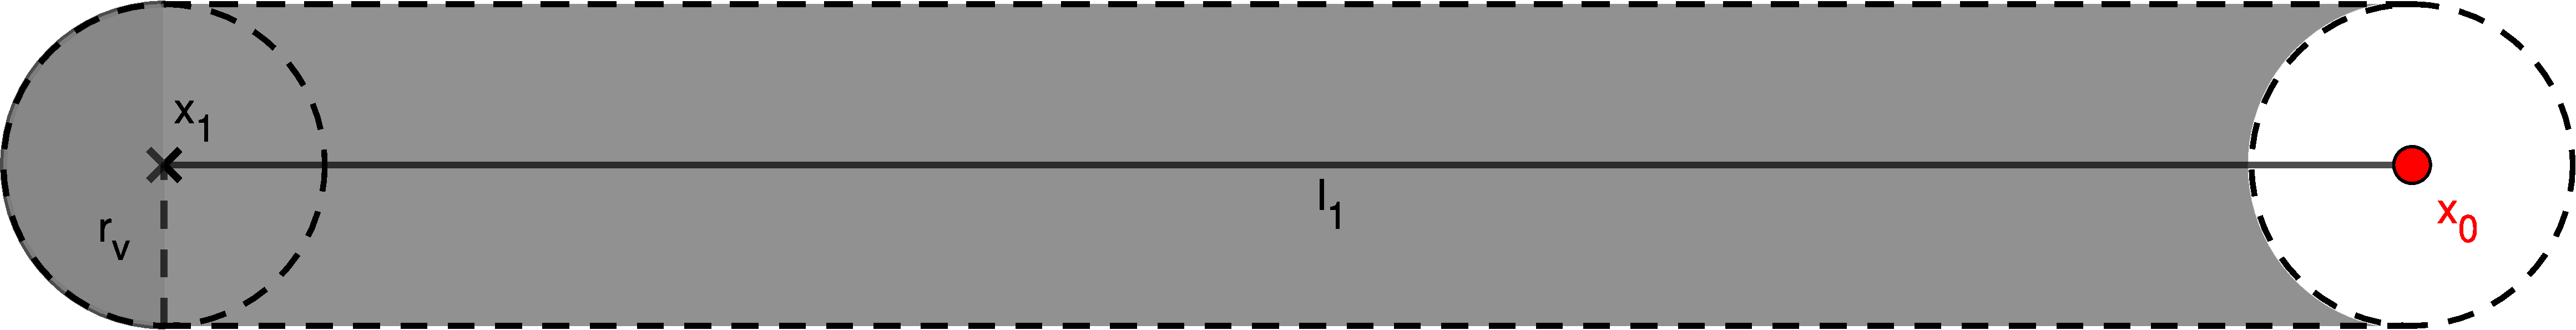
\includegraphics[width=1.0\textwidth]{2D-0thOrderApproximation-crop}
	\caption[Area covered by a step in the zeroth-order model]{A step from location $x_0$ to $x_1$. The search area that is explored by the forager is shaded in grey. The initial circle of radius $r_v$ around the forager is known to be empty, otherwise the forager's search would have ended during the previous step. \label{fig:2dbless:searcharea}}
\end{figure}

\begin{figure}[h!]
	\centering
	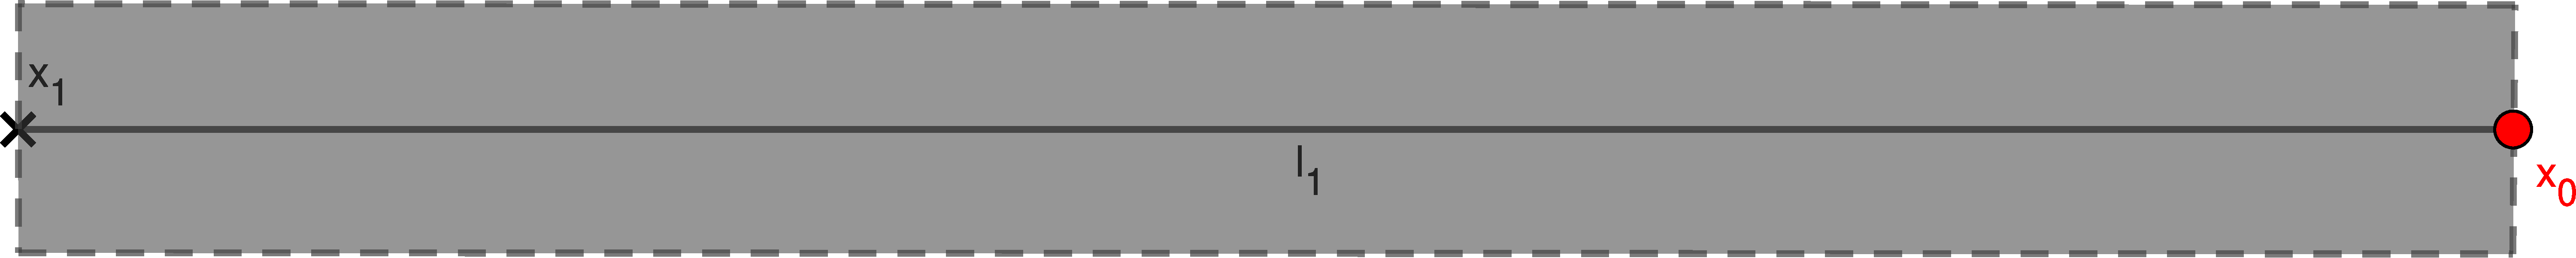
\includegraphics[width=1.0\textwidth]{2D-0thOrderApproximation_rectangles-crop}
	\caption[Area covered by a step in the zeroth-order model, simplified into a rectangle]{A step from location $x_0$ to $x_1$. The search area that is explored by the forager is shaded in grey, and has now been simplified into a rectangle by not taking into account the radius of vision around the forager at either end of a step. The total area is still the same. \label{fig:2dbless:searcharea_rectangle}}
\end{figure}



Since $\ell$ is a random variable, $A$ is also a random variable, which in our case is
\begin{equation*}
f_A(a) = \frac{f\left( \frac{a}{2r_v}\right)}{2r_v}.
\end{equation*}
The probability of not finding food, from \cref{eq:2d_prob_not_found}, was
\begin{align*}
\Pr(\text{not found}) &=\int_{A_{\min}}^\infty e^{-a\rho} f_A(a)da\\
& =\int_{A_{\min}}^\infty \frac{e^{-2r_v\ell\rho}}{2r_v} f\left(\frac{\ell}{2r_v}\right)d\ell,
\end{align*}
for which integration by substitution yields
\begin{equation}
\label{eq:2dbless:not_found_prob}
\Pr\left(\text{not found}\right) = \int_{\lmin}^\infty e^{-2 \ell r_v \rho} f(\ell)d\ell,
\end{equation}
which can now be solved exactly, depending on the step-length distribution.

Since the probability of finding food is the same for every step under our zeroth-order model, we can consider $\tau$ as a geometric random variable. 
 
The fact that $\tau$ is geometrically distributed also tells us that the expectation of the total number of steps is
\begin{equation}
\label{eq:2d_model:EN}
\E{N} = \frac{1}{\Pr(\text{found})} = \left( 1-  \int_{\lmin}^\infty e^{-2 r_v \ell \rho} f(\ell)d\ell \right)^{-1},
\end{equation}
which is used in evaluating the efficiency.

Recall \cref{eq:2d_El_split}, 
\begin{equation*}
\E{\ell_T \mid \ell} = \int_{\beta=0}^{2 \pi}\int_{u = 0}^{\ell} \rho A(u,\beta) e^{- \rho A(u,\beta)} \frac{1}{2\pi}  du d\beta +  \ell \int_{\beta=0}^{2 \pi}  \left(e^{-\rho A(u,\beta)}\right) \frac{1}{2\pi}  d\beta,
\end{equation*}
which gives us an expression for the expected step-length of a single step. For the zeroth-order approximation, this becomes
 \begin{align*}
\E{\ell_T \mid \ell} &= 2 r_v \rho \int_{u = 0}^{\ell} u e^{-2 r_v u \rho} du +  \ell e^{-2 r_v \rho \ell}\\
&=2 r_v \rho \left[\frac{-e^{-2r_v\rho u}(2r_v \rho u + 1) }{(2r_v\rho)^2}\right]_{0}^\ell  + \ell e^{-2 r_v \rho \ell}\\
&= \frac{1 -e^{-2r_v\rho \ell}(2r_v \rho \ell + 1) + 2r_v \rho \ell e^{-2r_v\rho \ell}}{2r_v\rho}\\
&= \frac{1 -e^{-2r_v\rho \ell}}{2r_v\rho}.
\end{align*}

Substituting this back into \cref{eq:2d_El}, we get
\begin{align*}
\E{\abs{\ell}} &= \int_{\lmin}^\infty \left( \frac{1 - e^{-2r_v \rho \ell}}{2r_v \rho} \right) f(\ell) d\ell\\
&=\frac{1}{2 r_v \rho} \left( 1 - \int_{\lmin}^\infty e^{-2r_v \rho \ell} f(\ell) d\ell \right).
\end{align*}

Now, we have expressions for both the expected number of steps, and the length travelled in a single step, so we can find the efficiency. Note that,
\begin{align*}
\E{N}\E{\abs{\ell}} &= \left( 1-  \int_{\lmin}^\infty e^{-2 r_v \ell \rho} f(\ell)d\ell \right)^{-1} \frac{1}{2 r_v \rho} \left( 1 - \int_{\lmin}^\infty e^{-2r_v \rho \ell} f(\ell) d\ell \right)\\
&=\frac{1}{2r_v\rho},
\end{align*}
and hence
\begin{equation}
\label{eq:2dmodel:0th:efficiency}
\eta = \frac{1}{\E{N}\E{\abs{\ell}}} = 2r_v\rho,
\end{equation}
meaning, as expected, that the efficiency of the zeroth-order approximation does not depend on the step-length distribution at all.
	
	With analytic expressions for the expected length of a step, as well as both the expected number of steps and the probability of finding a food within $n$ steps, we can now show that the two definitions of efficiency, \cref{eq:2d:efficiency,eq:2d:vis_efficiency}, are equivalent under the zeroth-order model.
	
	Recalling our expression for the expected total travel length, 
	\begin{align*}
	\E{L} &= \sum_{n=1}^\infty \E{\abs{\ell_n}} \left(\Pr(\tau \geq n )\right).
	\end{align*}
	Now, since the expected length of a single step, $\E{\abs{\ell}}$ does not depend on $n$, we may take it outside of the summation.
	\begin{equation*}
	\E{L} = \E{\abs{\ell}} \sum_{n=1}^\infty \Pr(\tau \geq n ),
	\end{equation*}
	which is equivalent to
	\begin{equation*}
	\E{L} = \E{\abs{\ell}} \E{N}.
	\end{equation*}
	Thus, our definition of efficiency is
	\begin{equation*}
	\eta = \frac{1}{\E{L}} = \frac{1}{ \E{\abs{\ell}} \E{N}},
	\end{equation*}
	which is equivalent to the definition of Viswanathan \etal \cite{Viswanathan_1999}. 
	%What we have shown is that in our model there is no covariance between the length of a step and the number of steps to find food.
	
\begin{example}
	We consider a forager with an exponential step-length distribution,
	\begin{equation*}
	p(\ell) = \mu e^{-\mu (\ell - \lmin)}, \quad \ell \in [\lmin,\infty), \, \mu >0.
	\end{equation*}
	Then, the probability that a step does not find a food target is
	\begin{align*}
	\Pr(\text{not found}) &= \int_{\lmin}^\infty e^{-2\ell r_v \rho} p(\ell) d\ell\\
	&=\int_{\lmin}^\infty  \mu  e^{-(2r_v \rho + \mu) \ell + \mu \lmin} d\ell\\
	&= \mu e^{\mu \lmin} \left[ \frac{e^{-(2r_v\rho + \mu) \ell}}{-(2r_v \rho + \mu)} \right]^\infty_{\lmin}\\
	&= \mu e^{\mu \lmin} \frac{e^{-(2r_v \rho + \mu) \lmin}}{2r_v\rho + \mu}\\
	&=\frac{ \mu e^{-2r_v \rho \lmin}}{2r_v \rho + \mu} ,
	\end{align*}
	and hence
	\begin{equation*}
	\left(\Pr(\text{not found})\right)^n = \left(\frac{ \mu e^{-2r_v \rho \lmin}}{2 r_v \rho + \mu}\right)^n.
	\end{equation*}
	
	
	Then, the probability of a food target being found on any given step is given by
	\begin{equation*}
\Pr(\text{found}) = 1 - \frac{ \mu e^{-2r_v \rho \lmin}}{2r_v \rho + \mu} = \frac{ 2r_v\rho + \mu -\mu e^{-2r_v \rho \lmin}}{2r_v \rho + \mu}.
	\end{equation*}
	
	Finally, the expected total number of steps to find a food target is
	\begin{align*}
	\E{N} = \frac{1}{\Pr(\text{found})  } = \frac{2 r_v \rho + \mu}{2r_v\rho + \mu -\mu e^{-2r_v \rho \lmin}}.
	\end{align*}
	
	Consider the case of $\mu \gg r_v \rho$, which corresponds to an average step size that is relatively small compared to the radius of vision and the food target density. For this case, $\Pr(\text{not found}) \approx e^{-2 r_v \rho \lmin}$, and hence $\E{N} \approx \frac{1}{1-e^{-2 r_v\rho \lmin}}$. Then, the smaller $r_v$, $\rho$ and $\lmin$ are, the greater the total number of expected steps, which makes intuitive sense.
	
The expected length of a single step is
	\begin{align*}
	\E{\abs{\ell}} &= \frac{1}{2r_v \rho} \left( 1 - \int_{\lmin}^\infty e^{-2r_v \rho \ell} p(\ell) d\ell \right)\\
	&= \frac{1}{2r_v \rho} \left( 1 - \int_{\lmin}^\infty e^{-2r_v \rho \ell} \mu e^{-\mu(\ell -\lmin)} d\ell \right)\\
	&= \frac{1}{2r_v \rho} \left( 1 - \mu e^{\mu \lmin} \int_{\lmin}^\infty e^{-(2r_v \rho + \mu) \ell} d\ell \right)\\
	&=\frac{1}{2r_v \rho} \left( 1 - \mu e^{\mu \lmin} \left[ \frac{e^{-(2r_v \rho + \mu)\ell}}{-(2r_v \rho + \mu)} \right]_{\lmin}^\infty \right)\\
	&=\frac{1}{2r_v \rho} \left( 1 - \frac{\mu e^{-2r_v\rho \lmin}}{2r_v \rho + \mu} \right).
	\end{align*}
	
	Then, unsurprisingly we get 
	\begin{equation*}
	\eta = \frac{1}{\E{N} \E{\abs{\ell}}} = {2r_v\rho}.
	\end{equation*}
\end{example} 

\subsection{First-order approximation}
\label{sec:2d:1storder}
We now consider the first-order approximation, which is considerably more difficult to solve.
Since the previous area must be taken into account overlap will occur, and thus the area will now also be a function of the turning angle.
As can be seen in \cref{fig:2d_model:firstorder:fourcases}, there are four separate cases to consider when determining the area of overlap, for a turning-angle of $0 \leq \beta \leq \pi$.
There are a further four cases for when the turning-angle is $\pi \leq \beta \leq 2\pi$, although these are mirrors of the first four cases, and only need a minor adjustment to ensure the sign of the trigonometric identities in the expressions are correct. 

\begin{figure}[h!]
	\centering
	\subfloat[{Case 1: A large turning-angle with large $\ell_2$}]{%
		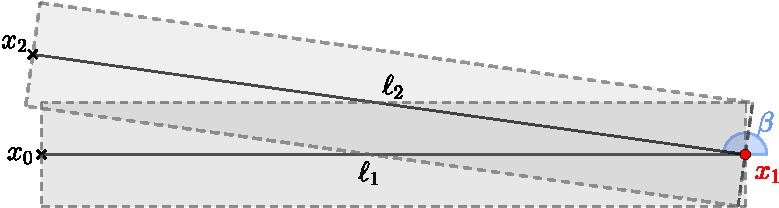
\includegraphics[width=.45\textwidth]{2D-1stOrderApproximation_rectangles_largeTA_largel2_nolabels-crop}}\hfill
	\subfloat[{Case 2: A large turning-angle with small $\ell_2$}]{%
		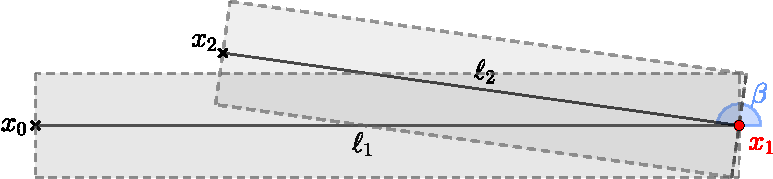
\includegraphics[width=.45\textwidth]{2D-1stOrderApproximation_rectangles_largeTA_smalll2_nolabels-crop}}\\
	\subfloat[Case 3: A medium turning-angle]{%
		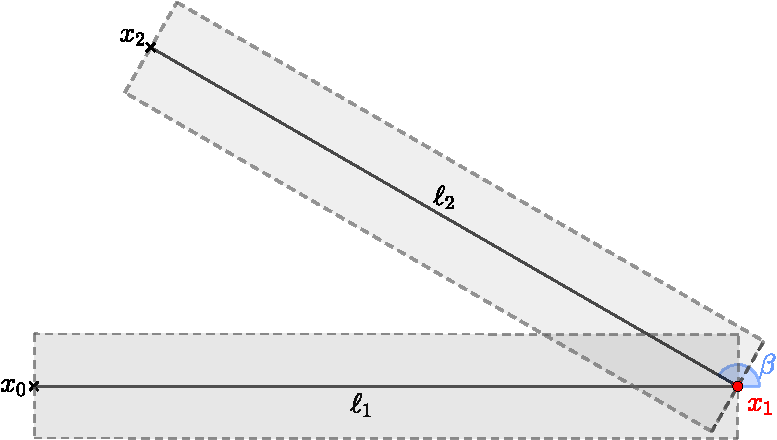
\includegraphics[width=.5\textwidth]{2D-1stOrderApproximation_rectangles_mediumTA_nolabels-crop}}\hfill
	\subfloat[Case 4: A small turning-angle]{%
		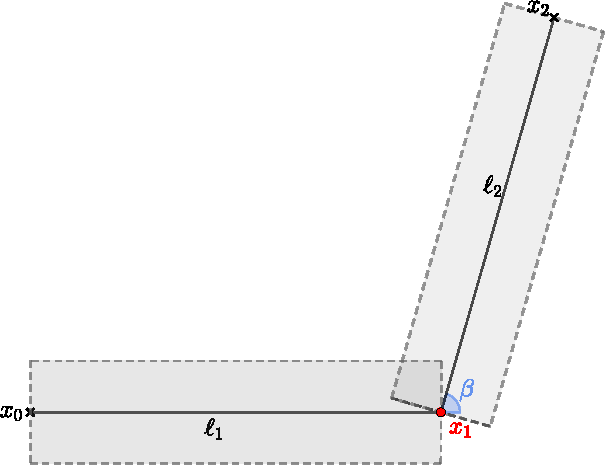
\includegraphics[width=.5\textwidth]{2D-1stOrderApproximation_rectangles_smallTA_nolabels-crop}}
	\caption[The four different cases for the turning-angle that we consider when determining the area of overlap]{The four cases that need to be considered to determine the overlapping area between two steps, with different turning-angles giving rise to different cases. When the turning-angle is large, which of case $1$ or case $2$ arise depends on the relative sizes of $\ell_1$ and $\ell_2$. When $\ell_2$ is sufficiently small, case $3$ becomes case $2$. Four more cases exist for turning-angles greater than $\pi$, although these are mirrors of the four cases above.}\label{fig:2d_model:firstorder:fourcases}
\end{figure}

Throughout the derivation of the area, we are forced to make some further simplifications in order to be able to realistically solve the problems. For example, there is actually more than $4$ cases to consider, since there is a separate case in between case $1$ and case $2$, although this only occurs at very specific angles and is similar in size to both of these two, so we exclude this. There are also times where we assume that very small triangles of area are right-angled, or else the expressions for the area would be far more complicated for little difference in accuracy. We use Monte Carlo simulations in \cref{sec:2dmodel:simulations:MC_area} to ensure our expressions for the area are suitably accurate. 

Even with these simplifications, deriving expressions for the area covered by a step is quite tedious and results in complicated expressions. 
For this reason, we relegate the derivation of the first-order area to \cref{sec:2dmodel:1starea}.
The resulting expressions for the area of overlap between consecutive steps 
are
\begin{equation*}
A_{\text{overlap}} = 
\begin{cases}
r_v^2 \left|\tan(\beta/2)\right| \quad &\text{if } \beta \leq \pi/2 \text{ or } \beta \geq 3\pi/2,\\\\
\displaystyle \frac{r_v^2 \left|\sin(\beta)\right|}{1-\left|\cos(\beta) \right|} &\text{if } \pi/2  \leq \beta \leq  \pi-\arcsin\left( \frac{2r_v}{\min(\ell_1,\ell_2)} \right),\\
&\text{or }\pi+\arcsin\left( \frac{2r_v}{\min(\ell_1,\ell_2)} \right) \leq \beta \leq 3\pi/2\\\\
\displaystyle \frac{1}{2} \left[-\min(\ell_1,\ell_2)^2 \left|\tan(\beta)\right| \right. &\text{if }\pi-\arcsin\left( \frac{2r_v}{\min(\ell_1,\ell_2)} \right) \leq \beta\\
\left.+ 2r_v \min(\ell_1,\ell_2)(2+\tan^2(\beta))\right.  &\text{and } \beta \leq \pi +\arcsin\left( \frac{2r_v}{\min(\ell_1,\ell_2)} \right).\\
\left. - r_v^2 \left|\tan^3(\beta)\right| \right]   
\end{cases}
\end{equation*}

Then, the total area covered by a step of length $\ell_2$ with turning-angle $\beta$ and previous step-length $\ell_1$ is
\begin{equation}
\label{eq:2dmodel:1storder:area_analytic}
A = 2\ell_2 r_v - A_{\text{overlap}}.
\end{equation}


In \cref{sec:2dmodel:simulations:MC_area}, we use Monte Carlo simulations to show \cref{eq:2dmodel:1storder:area_analytic} is close to the true value of $A$.

\subsubsection{Probability density function of the new area covered}
Let $f_A(x)$ be the \ac{PDF} representing a forager taking a step that covers $x$ amount of new area. We can express this as
\begin{equation*}
f_A(x) = \int_{\ell_1=\lmin}^\infty \int_{\beta=0}^{2 \pi} f_A (x,\beta,\ell_1) d\beta d\ell_1,
\end{equation*}
where $\ell_1$ is the length of the forager's previous step, $\beta$ is the forager's turning angle, and $x$ is a function of $\ell_1$, $\ell_2$ and $\beta$. Since the turning angle and the length of a step are drawn independently, we can further rearrange this to get
\begin{equation}
\label{eq:2d_model:fa_conditional}
f_A(x) = \int_{\ell_1=\lmin}^\infty \int_{\beta=0}^{2 \pi} f_A(x \mid \beta,\ell_1) f_{TA}(\beta) f(\ell_1) d\beta d \ell_1,
\end{equation}
where $f_{TA}$ is the density of the forager's turning angle, and $f(\ell_1)$ is the \ac{PDF} of the forager's previous step. The area covered by a step is a piecewise function that depends on whether $\ell_1 < -\ell_2 \cos(\beta)$ or $\ell_1 \geq -\ell_2 \cos(\beta)$, so we could write it as two separate integrals:

\begin{multline*}
f_A(x) =  \int_{\ell_1=\lmin}^{\ell_2} \int_{\beta=0}^{2 \pi} f_A(x \mid \beta,\ell_1) f_{TA}(\beta) f(\ell_1)f(\ell_2) d\beta  d \ell_1\\
+ \int_{\ell_1=\ell_2}^\infty \int_{\beta=0}^{2 \pi} f_A(x \mid \beta,\ell_1) f_{TA}(\beta) f(\ell_1) f(\ell_2)d\beta  d \ell_1.
\end{multline*}

Then, we can further split up the integrals to get
\begin{multline*}
f_A(x) =  2 \int_{\ell_1=\lmin}^{\ell_2} \int_{\beta=0}^{\pi/2} f_A(x \mid \beta,\ell_1) f_{TA}(\beta) f(\ell_1) d\beta d \ell_1\\
+  2\int_{\ell_1=\lmin}^{\ell_2} \int_{\beta=\pi/2}^{\pi - \arcsin(2r_v/\ell_1)} f_A(x \mid \beta,\ell_1) f_{TA}(\beta) f(\ell_1)d\beta  d \ell_1\\
+  2 \int_{\ell_1=\lmin}^{\ell_2} \int_{\beta=\pi - \arcsin(2r_v/\ell_1)}^{\pi} f_A(x \mid \beta,\ell_1) f_{TA}(\beta) f(\ell_1) d\beta  d \ell_1\\
+2 \int_{\ell_1=\ell_2}^\infty \int_{\beta=0}^{\pi/2} f_A(x \mid \beta,\ell_1) f_{TA}(\beta) f(\ell_1) d\beta d \ell_1\\
+2\int_{\ell_1=\ell_2}^\infty\int_{\beta=\pi/2}^{\pi-\arcsin(2r_v/\ell_2)} f_A(x \mid \beta,\ell_1) f_{TA}(\beta) f(\ell_1) d\beta  d \ell_1\\
+2\int_{\ell_1=\ell_2}^\infty \int_{\beta=\pi-\arcsin(2r_v/\ell_2)}^{\pi} f_A(x \mid \beta,\ell_1) f_{TA}(\beta) f(\ell_1) d\beta d \ell_1,
\end{multline*}
where we have $6$ rather than $12$ different terms since we have multiplied each term by $2$ due to symmetry.
For the first term, note that $f_A(x \mid \beta, \ell_1) = 2r_v \ell_1 - r_v^2 \tan(\beta/2)$ by \cref{eq:2dmodel:1storder:area_analytic}. We can rearrange this expression to find the inverse
\[x = 2r_v \ell_2 - r_v^2 \tan(\beta/2) \implies \ell_2 = \frac{x+r_v^2 \tan(\beta/2)}{2r_v}.\]
Thus, we can replace $f_A(x \mid \beta, \ell_1)$ with $f \left(\frac{x+r_v^2 \tan(\beta/2)}{2r_v}\right)$.
We can do similarly for the other integrals.
However, note that the third and the sixth integrals have an expression for $A$ which cannot be inverted easily, meaning we must either make further simplifications or solve the integrals numerically.



After solving for $f_A(a)$, we then must substitute the result, along with our piecewise function $A$ into
\begin{equation*}
\Pr(\text{not found}) = \int_{A_{\min}}^\infty e^{-a\rho} f_A(a)da,
\end{equation*}
which is then used to find $\E{N}$. For the first-order model, every step except the first step has the same probability of finding food, and so if we account for this we can also consider $\tau$ as a geometric random variable.
We do not proceed any further with this process analytically since the remainder of the work is dependent on the choice of step-length distribution, as well as requiring integration over complicated expressions.

\subsubsection{Truncated step-length}

As with the zeroth-order model, we need to determine the expected truncated length of a step, given the forager was intending to step a distance $\ell$. 
However, in the first-order model this will depend on the size of the steps as well as the turning-angle and the radius of vision. 
The probability of finding a target depends on the amount of new area being searched, and so should depend heavily on the geometry formed by the current and previous step.
Recall that our expression for $A$, \cref{eq:2dmodel:1storder:area_analytic}, required that $\ell_2 \geq r_v$, meaning we do not have a valid expression for the amount of new area covered while the forager is travelling the first $r_v$ distance.
We can assume that these values are also valid for the first $r_v$ distance of a step, although this is shown to be fairly inaccurate in \cref{sec:2dmodel:simulations}.
This assumption would allow us to write down some integrals for the truncated step-length, though we would not be able to solve them.

\subsubsection{Efficiency}

Although we have not been able to solve the first-order model analytically, we can draw some conclusions from the expressions we have found. Consider first the case when $\ell_1 < \ell_2$. The first two intervals for the area of overlap, for small and medium angles, have no dependence on $\ell_1$ or $\ell_2$, apart from changing when an angle is considered large. The area of overlap in the final interval, for large angles, will depend on the length of the previous step, $\ell_1$, since it is the smaller of the two steps. Thus, once $\ell_2$ gets larger than $\ell_1$, the area of overlap does not change. The total amount of new area will still increase as $2r_v\ell_2$. When $\ell_2 \leq \ell_1$, the total amount of overlapping area is similar for small and medium angles. The amount of overlapping area for large angles is very large, and increases as $\ell_2$ increases. Thus, we can conclude that to maximise the amount of new area covered, a forager should take steps as large as possible, regardless of what the previous step was. This would correspond to, for example, an exponential distribution with $\mu \to 0$ or a power-law distribution with $\mu \to 1$, which matches known results for destructive foraging.


\section{Simulations}
\label{sec:2dmodel:simulations}
\subsection{Monte Carlo simulations for the first-order area}
\label{sec:2dmodel:simulations:MC_area}
We use Monte Carlo simulations to estimate the true value of $A$, and compare with the results of our analytic expression. We first define the rectangle of search area from the previous step, at the following points in clockwise order: $(-\ell_1,r_v)$, $(0,r_v)$, $(0,-r_v)$, and $(-\ell_1,-r_v)$. Then,we can generate points in the area of the second step to determine the area of overlap. For some fixed $\ell_2$ and turning-angle $\beta$, we choose a uniformly distributed random variable $u_1$, between $0$ and $\ell_2$, and can then define the point $(u_1 \cos(\beta),u_1 \sin(\beta))$. This point is some random point along the path of the forager's current step. Next, we randomly generate a uniformly distributed random variable $u_2$, between $-r_v$ and $r_v$, to represent any point along the perpendicular radius of vision. Thus, the final location of our point will be at $\left(u_1 \cos(\beta)+u_2\sin(\beta), u_1 \sin(\beta) - u_2 \cos(\beta)\right)$.

If the randomly generated point is within the rectangle of the previous step, it is overlapping with the previous step. We randomly generate $50000$ points using the above process, and can estimate the proportion of overlapping points as $n/50000$, where $n$ is the number of points that were overlapping. The total area of overlap will therefore be, $(n/50000) 2 r_v \ell_2$, and so the newly explored area is $A=2(50000-n)/n r_v \ell_2$. We take the Monte Carlo simulation to be the true value, and determine the relative error of the analytic expressions based on this. Implicit in this is the assumption that the Monte Carlo simulations produce the exact value for the area, which is not true, although relative to the error in our analytic expressions the Monte Carlo simulations produce very accurate values. \Cref{fig:OverlappingArea_example} shows an example of this. We repeat this whole process for various values of $\ell_1$, $\ell_2$, $r_v$, and $\beta$, and compare the found area of overlap with our analytic expressions \cref{eq:2dmodel:1storder:area_analytic}.

\begin{figure}[h!]
	\centering
	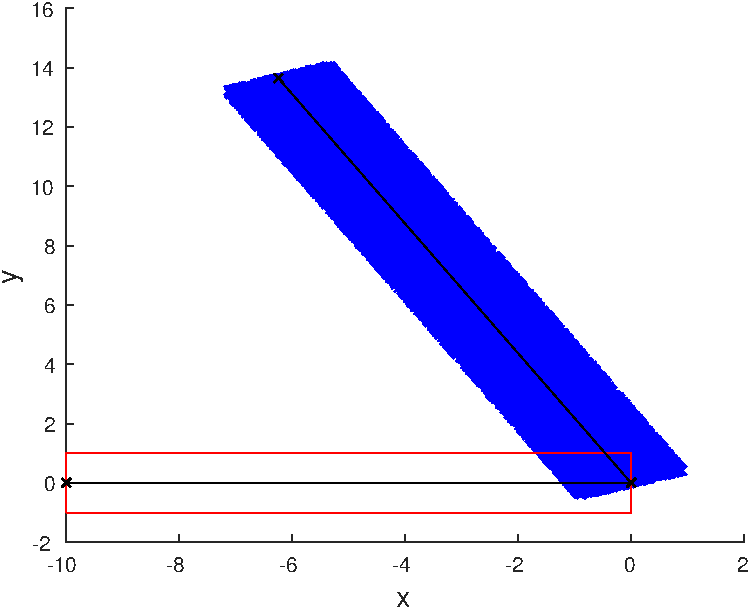
\includegraphics[scale=0.73]{OverlappingArea_10l1_15l2_1rv_2beta_50000reps}
	\caption[An example step where the overlapping area is approximated using a Monte Carlo simulation, and compared with our analytic expressions]{An example of our Monte Carlo simulation method to determine the amount of overlapping area between two consecutive steps, for $\ell_1=10$, $\ell_2 = 15$, $r_v=1$, and $\beta=2$. The area covered by the previous step is represented by the red rectangle, and each of the $50000$ simulated points are blue crosses. In this case, $n=243$ points overlap with the red rectangle, and the full area of the current step is $2r_v\ell_2 = 30$, so the area of overlap is $A=1.458$. The amount of total new area covered is $A=28.542$ according to this method, and $A=28.443$ according to our analytic approximation, giving a relative error of $0.0072$. \label{fig:OverlappingArea_example}}
\end{figure}

\begin{figure}[h!]
	\centering
	\subfloat[{Relative error vs. turning-angle $\beta$}]{%
		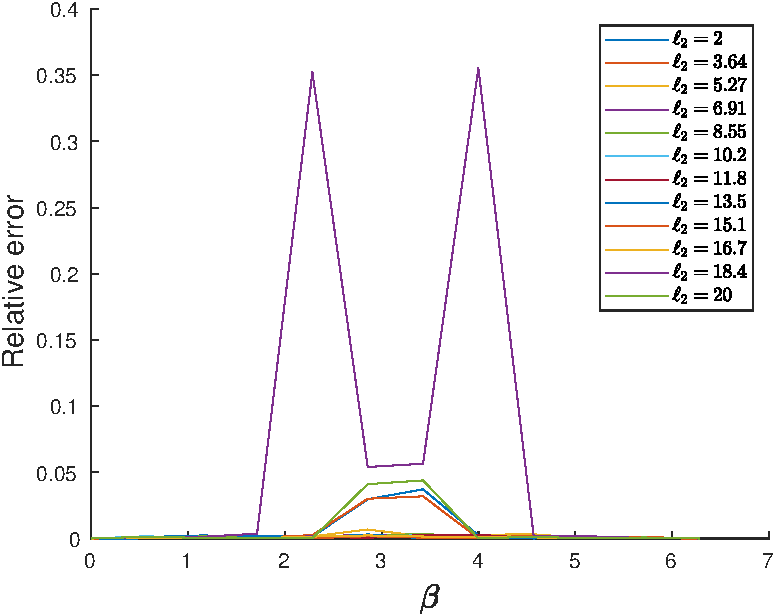
\includegraphics[width=.50\textwidth]{OverlappingArea_eVsbeta_10l1_1rv_50000reps}\label{fig:OverlappingArea_beta}}\hfill
	\subfloat[{Relative error vs step-length $\ell_2$}]{%
		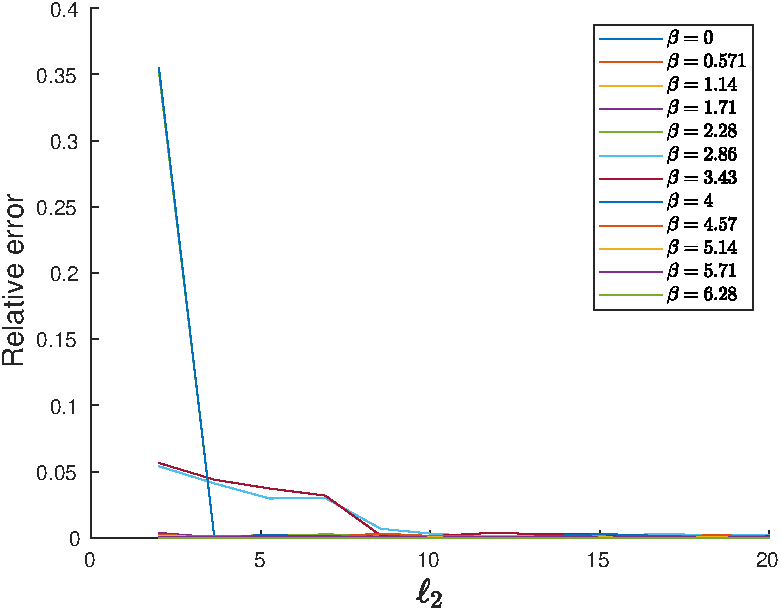
\includegraphics[width=.50\textwidth]{OverlappingArea_eVsl2_10l1_1rv_50000reps}\label{fig:OverlappingArea_l2}}\\
	\caption[The relative error in our analytic expressions for the overlap plotted against the step-length and the turning-angle]{The relative error plotted against the step-length $\ell_2$, for $2 \leq \ell_2 \leq 20$ at $10$ equispaced intervals and against the turning-angle $\beta$, for $0 \leq \beta \leq 2 \pi$.  The radius of vision is $r_v=1$ and $\ell_1 = 10$. Large relative errors occur at $\beta=2.86$ and $\beta=4$ take large values for small values of $\ell_2$, and all other values of $\ell_2$ and $\beta$ produce a relative error less than $0.065$.}\label{fig:OverlappingArea}
\end{figure}

Looking first at \cref{fig:OverlappingArea_beta}, we see that the relative error in the area is less than $0.05$ everywhere except for when $\ell_2 = 2$. When $\ell_2=2$, there are two large spikes in the relative error when $\beta = \approx 2.2$ and $\beta \approx 4.1$. The reason for the large error at these points are the assumption we made in \cref{app:area}, that $\ell_2 \gg r_v$, and $\ell_1 \approx \ell_2$, both of which are violated at these values, causing the wrong piecewise expression to be considered. This happens for these angles specifically because they are normally close to a threshold angle. Also looking at \cref{fig:OverlappingArea_l2}, we can draw the same conclusions, with a lower $\ell_2$ causing larger errors, as well as large errors occurring at $\beta = 0$, $\beta\approx 2.86$, and $\beta \approx 4.57$.

\begin{figure}[h!]
	\centering
	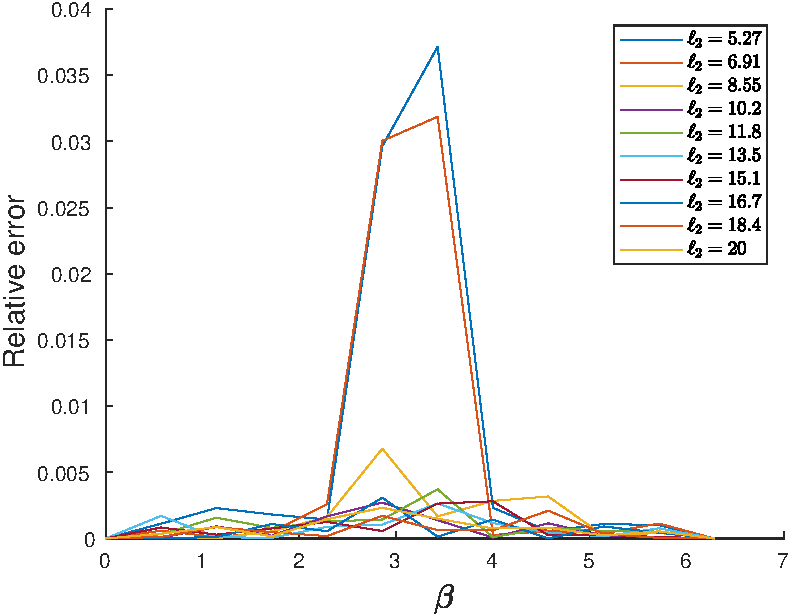
\includegraphics[scale=0.68]{OverlappingArea_eVsbeta_10l1_1rv_50000reps_skip2}
	\caption[The relative error in our analytic expressions for the overlap plotted against the turning-angle]{The relative error plotted against the turning angle $\beta$, for $0 \leq \beta \leq 2 \pi$ at $10$ equispaced intervals. The radius of vision is $r_v=1$ and $\ell_1 = 10$, and lines are plotted for $10$ different values of $\ell_2$, from $5.27$ to $20$. The lines for $\ell_2=5.27$ and $\ell_2 = 6.91$ has large peaks near the centre, for values of $\beta$ near $\pi$, corresponding to a large turning angle, and all other values of $\ell_2$ and $\beta$ produce a relative error less than $0.05$. \label{fig:OverlappingArea_beta_skip}}
\end{figure}

In \cref{fig:OverlappingArea_beta_skip} we plot the relative efficiency against the turning-angle as we did in \cref{fig:OverlappingArea_beta}, except we exclude the lowest two values of $\ell_2$. Now, the two lowest values of $\ell_2 = 5.27$ and $\ell_2=6.91$ produce the largest error, at $\beta \approx \pi$. The error at these points is less than $0.04$, and the cause for the error is the approximations made for the case of large turning-angles (case $1$) in \cref{app:area}. For all other values of $\beta$ and $\ell_2$, the relative error is lower than $0.01$, which is a good level of accuracy.

In summary, the analytic expressions from \cref{eq:2dmodel:1storder:area_analytic} are relatively accurate for most values of $\beta$ and $\ell_2$, with some larger errors occurring when $\ell_2$ is small and $\beta \approx \pi$. The effect that these points of inaccuracy will have on the overall calculation will depend on the turning-angle distribution as well as the step-length distribution. For example, a step-length distribution with a very large minimum step-size would always produce large steps and would not suffer from many of these inaccuracies. 


\FloatBarrier
\subsection{Simulating our two-dimensional model}
\label{sec:2dmodel:simulation}

We use Matlab to simulate the model outlined above. We initially use a $50 \times 50$ search space, and generate food targets according to a spatial Poisson point process on this search space, with density $\rho$. We simulate the Poisson process by first drawing a number $N \sim \mathcal{P}(50^2\rho )$, and then drawing $N$ random variables from $x \sim \text{Uni}[0,50]$ and $N$ random variables from $y \sim \text{Uni}[0,50]$, and pairing these up to form the coordinates of the targets.

The forager begins at the centre of the search space at $(25,25)$. To simulate the movement of the forager, we draw an angle with $\theta \sim \text{Uni}[0,2\pi]$ and a step-length from our step-length distribution using inverse transform sampling. Thus, we are able to simulate a series of coordinates corresponding to the foragers steps. When a forager steps outside of the search area, we extend the search area in multiples of $50$ until the foragers new location is within the search area, and generate new targets in the new area in the same way as above.

After each step is taken, we check to see if a target has been located. To do this, we determine the perpendicular distance that each food patch is away from the line segment connecting the start and end points of a step. If we wanted to consider the circle of vision at the start and end of each step, we could also check the distance each point is from these points, in any direction. However, for consistency with our analytic model we exclude these. If any of these distances are less than $r_v$, then a target is located on that step. The located target is the one that is closest to the starting point of the step.

\Cref{fig:TwoDForager_Exponential} shows a single simulation of our model, with the forager using an exponential distribution. This model currently corresponds to the infinite order foraging model since once an area has been explored unsuccessfully, there is no chance of finding points there when reexploring the area. To instead consider our zeroth-order approximation, each time a step fails to locate food we generate targets according to a Poisson distribution as done above, although this time only in the area that was just explored. For the first-order model, we also do this although there is a lag of $1$ step before each regeneration. We can then consider any $k$th-order approximation by setting the regeneration lag to $k$.

\begin{figure}[h!]
	\centering
	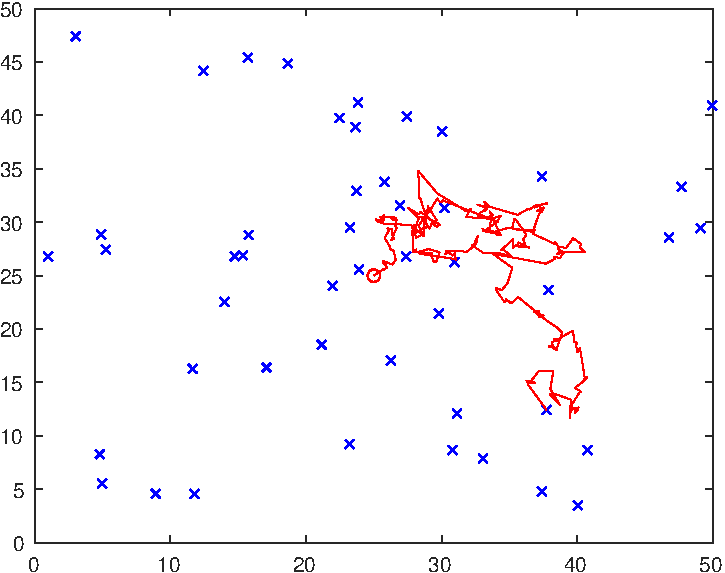
\includegraphics[scale=0.68]{TwoDForager_Exponential_0lmin_1-80mu_0-20rv_0-02rho}
	\caption[An example simulation of our two-dimensional]{A simulation of our two-dimensional foraging model, with parameters $r_v=0.2$, $\rho=0.02$. The forager takes steps from an exponential distribution with $\lmin=0$ and $\mu = 1.8$. No points are regenerated in areas that have already been explored, and thus this corresponds to the infinite order model. \label{fig:TwoDForager_Exponential}}
\end{figure}

\Cref{fig:TwoDForager_Efficiency_PowerLaw} compares the average step-length, mean number of steps, and efficiency, respectively, for the zeroth-order, first-order and infinite order models for a power-law forager. The efficiency of the simulated zeroth-order model matches the exact expression for the efficiency that we found, \cref{eq:2dmodel:0th:efficiency}. The efficiency of the first-order model decreases slightly as $\mu$ increases, and is slightly less efficient than the zeroth-order model, which is to be expected since targets are not being regenerated as quickly. The decrease in efficiency as $\mu$ increases also matches our conclusions from the analytic work on the first-order model, where we reasoned that the larger each step was, the less backtracking that would occur and hence more fresh area would be explored. Also, we are considering destructive foraging, for which it is known that ballistic motion offers the best efficiency (e.g. \cite{Viswanathan_1999}). 

The efficiency of the infinite order model decreases much faster than either the zeroth or first-order models. 
While the zeroth and first-order model seem to be fairly similar to each other, the infinite order model is significantly different to both, indicating that neither the zeroth or first-order models are accurate approximations for the infinite order model, and higher order models are needed. However, the first-order model is already too complicated to fully solve analytically, so an analytic approach to even higher order models is out of the question. Nonetheless, the zeroth-order and the first-order models can be considered as upper bounds for the infinite-order model. 


\begin{figure}[h!]
	\centering
	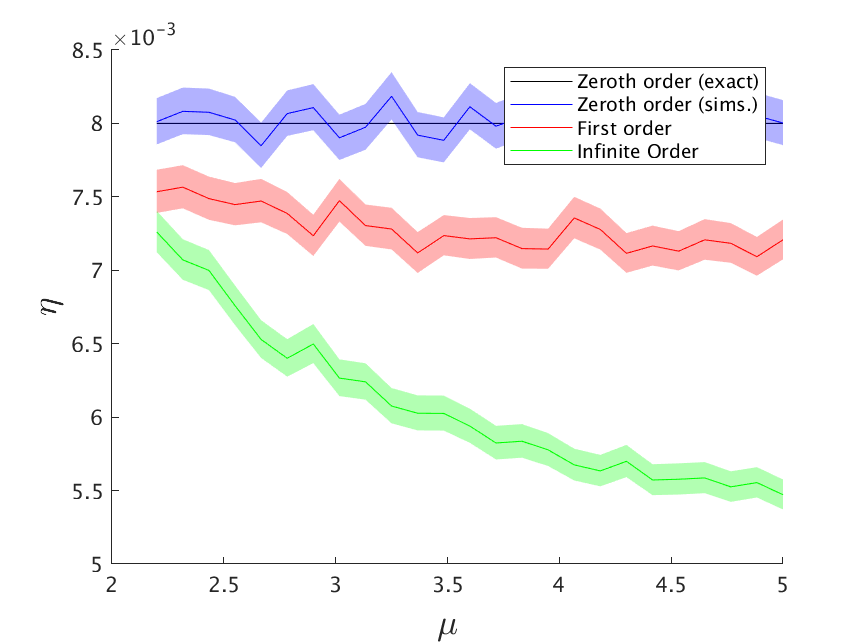
\includegraphics[scale=0.68]{TwoDForager_Efficiency_PowerLaw_1lmin_0-20rv_0-02rho_10000reps}
	\caption[Comparison of zeroth-order, first-order, and infinite-order model, and the analytic results for the zeroth-order]{The mean efficiency for the zeroth, first, and infinite order models with 95\% confidence intervals, as well as the exact result found for the zeroth-order model. The forager takes steps from a power-law distribution with $\lmin=1$, and for $25$ equispaced values of $\mu$ between $2.2$ and $5$. The mean is taken over $10000$ repetitions. \label{fig:TwoDForager_Efficiency_PowerLaw}}
\end{figure}
\end{chapter}

% Chapter 7: Conclusion
\begin{chapter}{Conclusion \label{sec:conclusion}}
%!TEX root = ../thesis.tex




In this thesis, we have considered an existing one-dimensional foraging model and derived expressions for the efficiency of a Markov-modulated random walk strategy. We have shown how these can be discretised and solved numerically. Using these expressions, results for the optimal efficiency were found for a range of different strategies, and we have discussed how some existing strategies can be seen as a special case of our Markov-modulated random walk strategy. We have confirmed the conclusions of these, and in some cases been able to extend the results. We also constructed a simple two-dimensional model and found some basic results about the efficiency of destructive foraging. We now recap the main findings of our thesis, as well as describe some future work.

\paragraph{\Cref{sec:1Dmodel}: One-dimensional foraging model}
This chapter was perhaps the most important. We began with an existing one-dimensional foraging model and first considered a random walk search strategy, for which results already exist \cite{Bartumeus_2013}. We proved a number of these results, such as the expected total distance travelled to find a target. Although already known, we have placed these results on more rigorous grounding. For example, we have shown explicitly that the operator norm of the integral operator we use is less than one, and hence convergence of the Neumann series is guaranteed. Further, we also found a separate expression for the expected total travel length which does not require a known starting location.

We then considered a Markov-modulated random walk search strategy, and derived analogues to the existing expressions for the random walk search strategy, such as the expected total travel length and the expected number of steps to find a target. More than just switching step-length distributions, we also allow the Markov chain to change the forager's radius of vision. One limitation of our expressions is that we are required to assume that the transition matrix does not depend on the forager's current location. A transition matrix that was a function of the forager's current location would actually allow us to investigate location-aware foragers, such as those of \cite{Nolting_2013}. This would represent a forager that changes strategy depending on where it is relative to a food patch, for which there is empirical evidence of this occurring \cite{Patterson_2017}. Another limitation is that our derivation requires a step-length distribution that is symmetric about zero. If we could consider non-symmetric step-length distributions, we could investigate the effects of an orientational memory by making movements in one direction more likely than the other.

\paragraph{\Cref{sec:1d_discrete}: Discretisation of the one-dimensional search space}
In this chapter, we discretised the one-dimensional model from \Cref{sec:1Dmodel}. Following a similar methodology as earlier, we once again use an operator, which we showed could be represented by a matrix $A$. We find discretised analogues of all of the important results from \Cref{sec:1Dmodel}, and discussed how they could be solved numerically in Matlab. The work of this chapter also helps to demonstrate some of the difficulties that arose in \cref{sec:1Dmodel}, since we are able to look at the problem in terms of matrices instead of integrals. In particular, the issue with finding the cost incurred in a single state rather than all states is easier to understand from the perspective of a discrete search space.


\paragraph{\Cref{sec:1d_results}: Results for the one-dimensional model}
In \cref{sec:1d_results}, we implemented the discrete expressions for the expected total area that we derived in \cref{sec:1d_discrete}, and investigated the efficiency of a range of different strategies. 
In \cref{sec:1dMMRW_nonMM}, we considered the unmodulated random walk, which is a special case of the Markov-modulated random walk, when the Markov chain has only a single state. We plotted the efficiency for four different step-length distributions: unbounded power-law, bounded power-law, unbounded exponential, and bounded exponential. For destructive foraging, the optimal strategy was to perform ballistic motion. For non-destructive foraging, ballistic motion was best for the unbounded and bounded exponential distributions, but for the two power-law distributions, a L\'{e}vy walk with $\mu \approx 2$ provided a higher efficiency. These results are all consistent with previous results found throughout the literature. 

We also investigated the effect that the upper bound has on the search efficiency. For both the exponential and power-law distributions, the upper bound caused a lower efficiency, and the lower the upper bound was, the worse the efficiency became.

In \cref{sec:1dMMRW_GUT}, we showed how giving-up time strategies could be modelled using our Markov-modulated random walk strategy, by constructing the transition matrix to have an absorbing state. Thus, we reasoned that we could use our Markov-modulated random walk model to consider any discrete phase-type distribution for the giving-up time, and could in theory construct our transition matrix in such a way as to approximate any giving-up time distribution, since the phase-type distribution is dense in the field of all positive-valued distributions. However, for accurate approximations, we may require using Markov chains with a large number of states, which quickly becomes computationally infeasible.

We considered a Brownian motion giving-up into a ballistic motion, and found the giving-up time parameter which optimised the efficiency. Our results are relatively close to the existing results by Plank and James \cite{Plank_2008}, given the significantly different approaches taken between us and them. 

Next, we fixed the giving-up time and investigated the optimal choice of step-length distribution parameters. We found that a Brownian motion that gives up and performs a L\'{e}vy flight is the most efficient, matching the results of Reynolds \cite{Reynolds_2009_adaptive}. The optimal parameter of the L\'{e}vy flight depends on the giving-up time, and the faster a forager gives up the larger $\mu$ should be, with a maximum being $\mu \approx 2$, corresponding to when a forager instantly gives up which is essentially the same as using a single strategy.

Finally, for the giving-up time strategies, we optimised over both the giving-up time parameter and the step-length distribution parameters, for a two-state strategy. This combines the best of both of the two previously mentioned papers on giving-up time strategies. We found the optimal efficiency occurred when the forager began with a Brownian motion with $\mu$ as large as possible, and gave up after a geometrically distributed time ($p=0.0060$, mean of $166.6$) and performed a L\'{e}vy flight with $\mu_2 = 1.5868$. As far as we are aware, there is no existing literature that has optimised over both the step-length parameters and the giving-up time at the same time.

We also discussed how we could consider various vision-switching strategies, in \cref{sec:1dMMRW_VisionSwitching}. We outlined how models with hidden or hard-to-detect targets could be approximated using our model, although this is computationally infeasible for heavy-tailed distributions, making this not very useful. Simpler models in which the forager's radius of vision switches at various times, which perhaps represents switching between different weather conditions, can easily be modelled with our Markov-modulated random walk strategy. We plotted an example of this, showing how a switching vision skews the symmetrical plot of step-length parameters against searching efficiency for a forager with equal probabilities of switching between each state. Since a model like this is very animal-specific and dependent on the choice of parameters, we do not determine any results for the optimal vision-switching forager.

Finally, in \cref{sec:1dMMRW_all} we investigated the most general models thus far, the Markov-modulated random walk, with any parameters for the transition matrix, initial distribution and step-length parameters. We began with a one-state model, and explain how we can construct a $J$-state model, showing that this involves $J^2+J-1$ parameters to optimise over. We used Matlab's \emph{fmincon} function to determine the parameters that result in the optimal efficiency for the $1$-state, $2$-state, and $3$-state strategies. We also outlined a method for selecting a reasonable starting point for the optimisation, which uses the results of the previous solution.

The optimal solution for the $1$-state model simply reiterated the results that we found for the unmodulated random walk, which is $\mu = 1.8699$. For the $2$-state model, we found something more interesting. The optimal strategy was to begin with a Brownian motion before switching into a L\'{e}vy flight with $\mu=1.5868$, with the transition matrix having an absorbing state, and initial distribution $(1,0)$. This is exactly the optimal two-state giving-up time strategy found earlier. Thus, we are able to conclude that giving-up time strategies are optimal for $2$-state Markov-modulated random walks. For the $3$-state model, we once again find that a giving-up time strategy is optimal. The optimal transition matrix was found to be
\begin{equation*}
P = \begin{bmatrix}
0.9849  &  0 &   0.0151\\
0  &  1  &  0\\
0 &  0.0152   & 0.9848
\end{bmatrix},
\end{equation*}
with an initial probability vector $\vec{z_{0}} = (1,0,0)$, and distribution parameters $\vec{\mu} = (10, 1.3908,    2.4368)$. This strategy once again corresponds to a giving-up time strategy that begins following a Brownian motion, before giving-up into a L\'{e}vy flight, with parameter $\mu = 2.4368$. Then, after some further time, the forager gives up again, and switches to a L\'{e}vy flight with $\mu = 1.3908$, which will somewhat resemble a ballistic path, due to the small $\mu$ parameter. The mean of the both geometrically distributed giving-up times is approximately $66$ steps. 

We hypothesise that the optimal intermittent strategies will always be giving-up time strategies. Further, we suspect that a $J$-state model will involve $J-1$ times at which the forager gives up into a different state, with no switching back to previous states. The $\mu$ parameters of these states will decrease each time a forager gives up. If this hypothesis is correct, it may perhaps also point to a potential optimal strategy in which a forager begins following a Brownian motion and $\mu$ decays continuously over time.

\paragraph{\Cref{sec:2dmodel}: Two-dimensional model}
In \cref{sec:2dmodel} we constructed a simple two-dimensional foraging model with targets distributed with complete spatial randomness. In order to find some analytic results, we introduced a simplifying assumption about target regeneration in areas that have already been explored. When targets can regenerate in areas that were explored previously in the step immediately prior, we call it the zeroth-order model. Similarly, if targets can regenerate after a delay of one step, we call this the first-order model. The case of no regeneration is called the infinite-order model, which involves no approximation. 

We found some analytic results for the efficiency of a random walk search strategy in the zeroth-order, which happens to not depend on the choice of step-length distribution at all. This result also corresponds to an upper bound for the efficiency of a strategy. For the first-order model, there is overlap between consecutive steps so we discussed the area of overlap as a function of the turning-angle and the step-lengths. We found approximate expressions for the area of a step, and use Monte Carlo simulations to ensure these are accurate. Ultimately, the expressions for the area are still too complicated to arrive at analytic expressions for the efficiency under the first-order model, though we can conclude that distributions with larger step-lengths will offer the highest efficiency, matching existing results. 

Finally, we simulated the zeroth-order, first-order, and infinite-order model numerically, and show that the first-order model does not actually offer a very good approximation of the infinite-order model anyway. We also argued that for analytic results to be found, much simpler two-dimensional models should be considered, such as lattice models.

\section{Future Work}
As discussed above, our work in \Cref{sec:1Dmodel} required an assumption that the transition matrix did not depend on the forager's current location, preventing us from considering location-aware foragers. However, our model may perhaps still be able to be used in investigating location-aware foragers, by making some extensions. In the location-aware forager of Nolting \cite{Nolting_2013}, the search area is divided into three sections, and the forager would use a different strategy in the left and right sections than the one it used in the middle section. One possible way we could consider this is by actually considering this as multiple separate searches, with the boundaries of the middle section representing a change of strategy rather than a food target. However, this would also require changes to the way our truncation is performed, as well as knowing more about whether it is the left or the right boundary that is found throughout a search.

In terms of considering non-symmetric step-length distributions in order to introduce an orientational memory, there are some possible avenues to explore. There are some key moments throughout \Cref{sec:1Dmodel} at which the symmetry is needed, in particular, after the introduction of the Dirac delta function. However, recall that we also found expressions that did not require a known starting location, so perhaps the symmetry assumption may be relaxed. This will require more investigation, and  will also need to consider how this will affect the discretisation of the step-length distributions, as well as any restrictions introduced to ensure that the operator norm is less than unity.

Recall from \cref{sec:1d_results} that we outlined a way to approximate the hidden targets model, although it was not adequate. This is because even when our forager has a vision radius of $0$, it may still reach the food by running into the target. To alleviate this problem, we can introduce periodic boundary conditions on the interval $[0,\lambda]$. Then, a food target would only be found if the forager landed with the food within its radius of vision, meaning it could skip over targets. To do this, we would have to adjust our expression for $\rho_n(x_n)$, and we now have to consider the previous location $\rho_{n-1}(x_{n-1})$ coming from any other interval, not just the current interval. This will introduce an infinite summation into the $\rho_n(x)$ recursive relation, which will not necessarily converge quickly when we consider heavy-tailed step-length distributions. 

In \cref{sec:1d_results}, apart from the unmodulated strategies, we only considered unbounded power-law distributions. This is because the other step-length distributions we considered offered worse performance in the unmodulated case. However, they may still offer better efficiency when considering switching strategies. No further extensions are required to test these out, though there are many possible combinations to consider, which can take a fairly long time to run. Similarly, we can consider $4$-state and higher Markov-modulated random walk models, which are also possible using our existing work, though slow computationally.

Further, we could also consider other distributions than the four we have investigated throughout this thesis. Our reasoning in choosing these four was that they are the only four that have been commonly used throughout the literature. However, more recent papers (e.g \cite{Bertrand_2015}) have considered a generalized Pareto distribution, of which Normal, exponential, and power-law distributions are special cases.

In terms of two-dimensional models, further work should first focus on simulations. Further investigation should be made into which one-dimensional results hold in higher dimensions. The model we outline in \cref{sec:2dmodel} could also be adjusted to account for non-destructive foraging in a few different ways. For example, rather than have a fully homogeneous spatial Poisson process, there could be different regions, representing areas that are either close or far from a previously visited target. Alternatively, the density of targets may be set high initially and made to decay over time, to represent the chance of reaching the previously visited target diminishing.

\end{chapter}

\appendix

% Import the appendices
%!TEX root = ../thesis.tex
\chapter{Calculating $h(x)$ and $A$ for some step-length distributions\label{app:calc}}
\section{Average step length\label{app:calc:ave_length}}

As demonstrated in \cref{sec:1dRW_distance}, the average step length for any given step-length distribution, where we are taking into account the possibility of truncation, is given by
\begin{equation}
\begin{split}
\label{eq:app_calc:ave_length}
\E{\abs{l}} &= \int_{-(a-r_v)}^{-\lmin} \abs{\ell} p(\ell) d\ell + \int_{\lmin}^{\lambda - r_v - a} \abs{\ell} p(\ell) d\ell\\
&+ (a-r_v)\int_{-\infty}^{-(a-r_v)} p(\ell) d\ell + (\lambda - r_v - a)\int_{(\lambda - r_v - a)}^\infty p(\ell)d\ell,
\end{split}
\end{equation}
where the first or second integral become zero for steps beginning near the boundaries at $r_v$ or $\lambda-r_v$, respectively. Similarly, the third and fourth integral's limits are adjusted slightly for steps beginning near either $r_v$ or $\lambda-r_v$, respectively.

Therefore, the average step length for each distribution will have three separate cases to consider, depending on the starting location of a step.

When the distribution also has an upper limit on the step size, $\lmax$, then we will also have to make further adjustments to the limits of integration, which will result in even more cases to consider.

We can rewrite \cref{eq:app_calc:ave_length} for this situation, as four separate cases, depending on the value of $\lmax$. Firstly, if $\lmax \geq a-r_v$ and $\lmax \geq \lambda-a-r_v$, we get
\begin{equation}
\begin{split}
\label{eq:app_calc:ave_length_lmax1}
\E{\abs{\ell}} &= \int_{-(a-r_v)}^{-\lmin} \abs{\ell} p(\ell) d\ell + \int_{\lmin}^{\lambda - r_v - a} \abs{\ell} p(\ell) d\ell\\
&+ (a-r_v)\int_{-\lmax}^{-(a-r_v)} p(\ell) d\ell + (\lambda - r_v - a)\int_{(\lambda - r_v - a)}^{\lmax} p(\ell)d\ell.
\end{split}
\end{equation}
If $\lmax \geq a-r_v$ and $\lmax < \lambda-a-r_v$,
\begin{equation*}
\begin{split}
\label{eq:app_calc:ave_length_lmax2}
\E{\abs{\ell}} &= \int_{-(a-r_v)}^{-\lmin} \abs{\ell} p(\ell) d\ell + \int_{\lmin}^{\lmax} \abs{\ell} p(\ell) d\ell\\
&+ (a-r_v)\int_{-\lmax}^{-(a-r_v)} p(\ell) d\ell.
\end{split}
\end{equation*}
If $\lmax < a-r_v$ and $\lmax \geq \lambda-a-r_v$,
\begin{equation*}
\begin{split}
\label{eq:app_calc:ave_length_lmax3}
\E{\abs{\ell}} &= \int_{-\lmax}^{-\lmin} \abs{\ell} p(\ell) d\ell + \int_{\lmin}^{\lambda - r_v - a} \abs{\ell} p(\ell) d\ell\\
&+ (\lambda - r_v - a)\int_{(\lambda - r_v - a)}^{\lmax} p(\ell)d\ell.
\end{split}
\end{equation*}
If $\lmax < a-r_v$ and $\lmax < \lambda-a-r_v$,
\begin{equation*}
\label{eq:app_calc:ave_length_lmax4}
\E{\abs{\ell}} = \int_{-\lmax}^{-\lmin} \abs{\ell} p(\ell) d\ell + \int_{\lmin}^{\lmax} \abs{\ell} p(\ell) d\ell.
\end{equation*}
We can also note that as $\lmax \to \infty$,  \cref{eq:app_calc:ave_length_lmax1} approaches \cref{eq:app_calc:ave_length} as expected.

These above expressions are valid when the forager is not near a boundary, that is, when $r_v + \lmin \leq a \leq \lambda - r_v - \lmin$. When the forager is close to the boundaries, we must adjust some of the limits of integration. Since the first two integrals in \cref{eq:app_calc:ave_length_lmax1} represent steps that land within the boundary, which aren't necessarily possible when next to the boundary, we must remove some of the integrals too.

For the left boundary, $r_v < a < r_v + \lmin$, we get when $\lmax \geq a-r_v$ and $\lmax \geq \lambda-a-r_v$,
\begin{equation*}
\begin{split}
\label{eq:app_calc:ave_length_lmax1_left}
\E{\abs{\ell}} &= \int_{\lmin}^{\lambda - r_v - a} \abs{\ell} p(\ell) d\ell + (a-r_v)\int_{-\lmax}^{-\lmin} p(\ell) d\ell\\
&+ (\lambda - r_v - a)\int_{(\lambda - r_v - a)}^{\lmax} p(\ell)d\ell.
\end{split}
\end{equation*}
If $\lmax \geq a-r_v$ and $\lmax < \lambda-a-r_v$,
\begin{equation*}
\label{eq:app_calc:ave_length_lmax2_left}
\E{\abs{\ell}} =\int_{\lmin}^{\lmax} \abs{\ell} p(\ell) d\ell + (a-r_v)\int_{-\lmax}^{-\lmin} p(\ell) d\ell.
\end{equation*}
The case of $\lmax < a-r_v$ and $\lmax \geq \lambda-a-r_v$ does not exist, since it would require $\lmax < \lmin$, and likewise for the case of $\lmax < a-r_v$ and $\lmax < \lambda-a-r_v$.

Based on these, we may also conclude that for a step-length distribution with no upper bound on the step size, at the left boundary we get,
\begin{equation}
\begin{split}
\label{eq:app_calc:ave_length_left}
\E{\abs{\ell}} &= \int_{\lmin}^{\lambda - r_v - a} \abs{\ell} p(\ell) d\ell + (a-r_v)\int_{-\infty}^{-\lmin} p(\ell) d\ell\\
&+ (\lambda - r_v - a)\int_{(\lambda - r_v - a)}^{\infty} p(\ell)d\ell.
\end{split}
\end{equation}

For steps near the right boundary, $\lambda-r_v-\lmin < a < \lambda -r_v$, we get when $\lmax \geq a-r_v$ and $\lmax \geq \lambda-a-r_v$,
\begin{equation*}
\begin{split}
\label{eq:app_calc:ave_length_lmax1_right}
\E{\abs{\ell}} &= \int_{-(a-r_v)}^{-\lmin} \abs{\ell} p(\ell) d\ell + (a-r_v)\int_{-\lmax}^{-(a-r_v)} p(\ell) d\ell\\
&+ (\lambda - r_v - a)\int_{\lmin}^{\lmax} p(\ell)d\ell.
\end{split}
\end{equation*}
If $\lmax < a-r_v$ and $\lmax \geq \lambda-a-r_v$,
\begin{equation*}
\begin{split}
\label{eq:app_calc:ave_length_lmax3_right}
\E{\abs{\ell}} &= \int_{-\lmax}^{-\lmin} \abs{\ell} p(\ell) d\ell\\
&+ (\lambda - r_v - a)\int_{\lmin}^{\lmax} p(\ell)d\ell.
\end{split}
\end{equation*}
The case of $\lmax \geq a-r_v$ and $\lmax < \lambda-a-r_v$ does not exist, since it would require $\lmax < \lmin$, and likewise for the case of $\lmax < a-r_v$ and $\lmax < \lambda-a-r_v$,

Based on these, we may also conclude that for a step-length distribution with no upper bound on the step size, near the right boundary we get,
\begin{equation}
\begin{split}
\label{eq:app_calc:ave_length_right}
\E{\abs{\ell}} &= \int_{\lmin}^{\lambda - r_v - a} \abs{\ell} p(\ell) d\ell + (a-r_v)\int_{-\infty}^{-\lmin} p(\ell) d\ell\\
&+ (\lambda - r_v - a)\int_{(\lambda - r_v - a)}^{\infty} p(\ell)d\ell.
\end{split}
\end{equation}

Thus, all up we have 8 different cases to consider for each distribution --- two near the left boundary, four in the centre, and two near the right boundary. If the distribution doesn't have a maximum step size, then we have only 3 cases to consider. Fortunately, all 10 cases are made up of combinations of integrals which only take 6 different forms, 3 of which are:
\begin{equation}
\label{eq:app1:intcase1}
\int_{c}^{d} \abs{\ell}p(\ell)d\ell, \quad c,d \in \mathbb{R}^+,
\end{equation}
\begin{equation}
\label{eq:app1:intcase2}
\int_{c}^{d} p(\ell)d\ell, \quad c,d \in \mathbb{R}^+,
\end{equation}
\begin{equation}
\label{eq:app1:intcase3}
\int_{c}^{\infty} p(\ell)d\ell, \quad c \in \mathbb{R}^+,
\end{equation}
and then, due to the symmetry of $p(\ell)$, the remaining three integrals are equivalent to integrals~\ref{eq:app1:intcase1},~\ref{eq:app1:intcase2}, and \ref{eq:app1:intcase3}, respectively:
\begin{equation}
\int_{-d}^{-c} \abs{\ell}p(\ell)d\ell, \quad c,d \in \mathbb{R}^+,
\end{equation}
\begin{equation}
\int_{-d}^{-c} p(\ell)d\ell, \quad c,d \in \mathbb{R}^+,
\end{equation}
\begin{equation}
\int_{-\infty}^{-c} p(\ell)d\ell, \quad c \in \mathbb{R}^+.
\end{equation}

Thus, finding the expected cost of a step for each step-length distribution amounts to not much more than solving integrals~\ref{eq:app1:intcase1},~\ref{eq:app1:intcase2}, and \ref{eq:app1:intcase3} and rearranging. Furthermore, for distributions \emph{without} an upper bound on the step size, integrals of the same form as integral~\ref{eq:app1:intcase2} never appear, and distributions \emph{with} an upper bound have no integrals of the same form as integral~\ref{eq:app1:intcase3}. 

As discussed in \cref{sec:1d_discrete}, to find the discretized equivalents of these expressions, we make the replacements:
\[\lmin = m_0 \Delta x, \quad \lmax = m_m \Delta x, \quad r_v = m_r \Delta x, \quad m_0,m_m,m_r \in \mathbb{Z}. \]

We find the exact expressions for the unbounded power-law distribution, and show that there are some small differences between our results and the expressions listed by Bartumeus \etal \cite{Bartumeus_2013}, which we explain is most likely due to a typo. We also present the discretized equivalents of the expressions for the unbounded power-law distribution. 

For the other step-length distributions, we simply present the solutions without showing any of the working.

\subsection{Unbounded power-law distribution}
Recall that an unbounded power-law distribution, where we allow both positive and negative values is:
\begin{equation*}
p(\ell) = C \abs{\ell}^{-\mu}, \quad \abs{\ell} \geq \lmin,
\end{equation*}
where \[C = \frac{(\mu - 1)}{2}\lmin^{\mu - 1}.\]
We can represent the support of the distribution by rewriting this as
\[p(\ell) =  C \left| \ell \right|^{-\mu} \theta(|\ell| - \lmin) , \]
and \[\theta(x) = \begin{cases}
		1 \quad &\text{if }x \geq 0,\\
		0 \quad &\text{otherwise}.
\end{cases}\]

For the unbounded power-law distribution, integral~\ref{eq:app1:intcase1} is given by
\begin{align*}
\int_{c}^{d} \abs{\ell} p(\ell) d\ell &= \int_{c}^{d}\frac{(\mu - 1)}{2}\lmin^{\mu - 1} \abs{\ell}^{1-\mu}  d\ell\\
&= \frac{(\mu - 1)}{2}\lmin^{\mu - 1} \int_{c}^{d} (\ell)^{1-\mu}  d\ell
\end{align*}
for $\mu \neq 2$:
\begin{align*}
\int_{c}^{d} \abs{\ell} p(\ell) d\ell  &= \frac{(\mu - 1)}{2}\lmin^{\mu - 1} \left[\frac{\ell^{2-\mu}}{2-\mu} \right]^{d}_{c}  \\
&= \frac{(\mu - 1)}{2}\lmin^{\mu - 1} \left[\frac{d^{2-\mu} - c^{2-\mu}}{2-\mu} \right]
\end{align*}
and for $\mu = 2$:
\begin{align*}
\int_{c}^{d} \abs{\ell} p(\ell) d\ell  &= \frac{\lmin}{2} \left[ \log(\ell) \right]^{d}_{c}  \\
&= \frac{\lmin}{2}  \left[\log(d) - \log(c)\right]\\
&= \frac{\lmin}{2}  \log\left(\frac{d}{c} \right).
\end{align*}
Integral~\ref{eq:app1:intcase3} is given by
\begin{align*}
\int_{c}^\infty p(\ell)d\ell &= \int_{c}^\infty \frac{(\mu - 1)}{2}\lmin^{\mu - 1} \abs{\ell}^{-\mu}d\ell\\
&= \frac{(\mu - 1)}{2}\lmin^{\mu - 1} \int_{c}^\infty  (\ell)^{-\mu}d\ell\\
&= \frac{(\mu - 1)}{2}\lmin^{\mu - 1} \left[\frac{\ell^{1-\mu}}{1-\mu} \right]_{c}^\infty \\
&=\frac{(\mu - 1)}{2}\lmin^{\mu - 1} \left[\frac{-c^{1-\mu}}{1-\mu} \right]\\
&=\frac{1}{2}\left(\frac{c}{\lmin}\right)^{1-\mu}.
\end{align*}

For the unbounded power-law distribution we have no upper bound on the step length, and hence there are only three cases to consider: near the left boundary, in the centre, and near the right boundary, which correspond to \cref{eq:app_calc:ave_length_left,eq:app_calc:ave_length,eq:app_calc:ave_length_right}, respectively. However, we do get two different expressions for each, depending on whether or not $\mu = 2$, making six expressions total.

For steps beginning near the left boundary, specifically for $r_v < a < r_v + \lmin$, when $\mu \neq 2$ we get
\begin{align}
\E{\abs{\ell}} &= \int_{\lmin}^{\lambda - r_v - a} \abs{\ell} p(\ell) d\ell + (a-r_v)\int_{-\infty}^{-\lmin} p(\ell) d\ell \nonumber \\
&+ (\lambda - r_v - a)\int_{(\lambda - r_v - a)}^{\infty} p(\ell)d\ell \nonumber \\ \nonumber\\
&= \frac{(\mu - 1)}{2}\lmin^{\mu - 1} \left[\frac{(\lambda-r_v-a)^{2-\mu} - \lmin^{2-\mu}}{2-\mu} \right]+ (a-r_v)\frac{1}{2}\left(\frac{\lmin}{\lmin}\right)^{1-\mu} \nonumber \\
&+ (\lambda - r_v - a)\frac{1}{2}\left(\frac{\lambda-r_v-a}{\lmin}\right)^{1-\mu}\nonumber \\ \nonumber \\
&= \frac{(a-r_v)}{2} + \frac{\lmin (1-\mu)}{2(2-\mu)} \left[ 1 + \frac{((\lambda-a-r_v)/\lmin)^{2-\mu}}{1-\mu} \right]\label{eq:app_calc:ave_step_length:powerlawL},
\end{align}
and when $\mu=2$ we get
\begin{align}
\E{\abs{\ell}} &= \frac{\lmin}{2} \left[ \log \left(\frac{\lambda - a-r_v}{\lmin} \right) + 1 \right] + \frac{(a-r_v)}{2}\nonumber \\
&= \frac{(a-r_v)}{2} + \frac{\lmin}{2} \left[ 1 + \log((\lambda-a-r_v)/\lmin) \right]\label{eq:app_calc:ave_step_length:powerlawL_mu2},
\end{align}
which agree with the expressions from Bartumeus \etal \cite{Bartumeus_2013}.


For the middle of the search space, which is valid for $r_v + \lmin \leq a \leq \lambda-r_v-\lmin$, when $\mu \neq 2$ we get
\begin{align}
\E{\abs{\ell}} &= \int_{-(a-r_v)}^{-\lmin} \abs{\ell} p(\ell) d\ell + \int_{\lmin}^{\lambda - r_v - a} \abs{\ell} p(\ell) d\ell \nonumber\\
&+ (a-r_v)\int_{-\infty}^{-(a-r_v)} p(\ell) d\ell + (\lambda - r_v - a)\int_{(\lambda - r_v - a)}^\infty p(\ell)d\ell \nonumber\\\nonumber\\
&= \frac{(\mu - 1)}{2}\lmin^{\mu - 1} \left[\frac{(a-r_v)^{2-\mu} - \lmin^{2-\mu}}{2-\mu} \right] + \frac{(\mu - 1)}{2}\lmin^{\mu - 1} \left[\frac{(\lambda-r_v-a)^{2-\mu} - \lmin^{2-\mu}}{2-\mu} \right]\nonumber\\
&+ (a-r_v)\frac{1}{2}\left(\frac{a-r_v}{\lmin}\right)^{1-\mu} + (\lambda - r_v - a)\frac{1}{2}\left(\frac{\lambda-r_v-a}{\lmin}\right)^{1-\mu} \nonumber \\ \nonumber \\
&= \frac{\lmin(1-\mu)}{2(2-\mu)}\left[ 2 + \frac{((a-r_v)/\lmin)^{2-\mu}}{1-\mu} + \frac{((\lambda - a- r_v)/\lmin)^{2-\mu}}{1-\mu} \right]\label{eq:app_calc:ave_step_length:powerlawM},
\end{align}
and for $\mu = 2$ we get
\begin{align}
\E{\abs{\ell}}&=\lmin \left[ 1 + \log \left(\frac{[(\lambda-a-r_v)(a-r_v)]^{1/2}}{\lmin} \right) \right]\label{eq:app_calc:ave_step_length:powerlawM_mu2}.
\end{align}
These two expressions are not consistent with Bartumeus \etal \cite{Bartumeus_2013}.

For steps beginning near the right boundary, specifically for $\lambda-r_v-\lmin < a < \lambda-r_v$, when $\mu \neq 2$ we get
\begin{align}
\E{\abs{\ell}} &= \int_{\lmin}^{\lambda - r_v - a} \abs{\ell} p(\ell) d\ell + (a-r_v)\int_{-\infty}^{-(a-r_v)} p(\ell) d\ell \nonumber \\
&+ (\lambda - r_v - a)\int_{\lmin}^{\infty} p(\ell)d\ell \nonumber\\ \nonumber \\
&= \frac{(\mu - 1)}{2}\lmin^{\mu - 1} \left[\frac{(\lambda-r_v-a)^{2-\mu} - \lmin^{2-\mu}}{2-\mu} \right]+ (a-r_v)\frac{1}{2}\left(\frac{a-r_v}{\lmin}\right)^{1-\mu}\nonumber \\
&+ (\lambda - r_v - a)\frac{1}{2}\left(\frac{\lmin}{\lmin}\right)^{1-\mu} \nonumber \\ \nonumber \\
&= \frac{(\lambda-a-r_v)}{2} + \frac{\lmin (1-\mu)}{2(2-\mu)} \left[ 1 + \frac{((a-r_v)/\lmin)^{2-\mu}}{1-\mu} \right]\label{eq:app_calc:ave_step_length:powerlawR},
\end{align}
and for $\mu = 2$ we get
\begin{align}
\E{\abs{\ell}} &= \frac{(\lambda -a-r_v)}{2} + \frac{\lmin}{2} \left[ 1 + \log((a-r_v)/\lmin) \right]\label{eq:app_calc:ave_step_length:powerlawR_mu2}.
\end{align}
These two expressions are also not consistent with Bartumeus \etal \cite{Bartumeus_2013}. However, after solving all three cases, we can now see that they have not made an error with their mathematics, but rather, have listed the middle expression as the left expression, and vice versa.

The discretized versions of  \cref{eq:app_calc:ave_step_length:powerlawL,eq:app_calc:ave_step_length:powerlawL_mu2,eq:app_calc:ave_step_length:powerlawM,eq:app_calc:ave_step_length:powerlawM_mu2,eq:app_calc:ave_step_length:powerlawR,eq:app_calc:ave_step_length:powerlawR_mu2} are listed below.


When $\mu \neq 2$, for the left, middle, and right sections, respectively:
\begin{equation*}
\label{eq:app_calc:ave_step_length:powerlawL_discrete}
\E{\abs{\ell}}_{i_a}= \frac{(i_a-m_r)\Delta x}{2} + \frac{m_0 \Delta x (1-\mu)}{2(2-\mu)} \left[ 1 + \frac{((M - i_a -m_r)/m_0)^{2-\mu}}{1-\mu} \right],
\end{equation*}

\begin{equation*}
\label{eq:app_calc:ave_step_length:powerlawM_discrete}
\E{\abs{\ell}}_{i_a} = \frac{m_0 \Delta x(1-\mu)}{2(2-\mu)}\left[ 2 + \frac{((i_a - m_r)/m_0)^{2-\mu}}{1-\mu} + \frac{((M - i_a -m_r)/m_0)^{2-\mu}}{1-\mu} \right],
\end{equation*}

\begin{equation*}
\label{eq:app_calc:ave_step_length:powerlawR_discrete}
\E{\abs{\ell}}_{i_a} = \frac{(M-i_a-m_r)\Delta x}{2} + \frac{m_0 \Delta x (1-\mu)}{2(2-\mu)} \left[ 1 + \frac{((i_a-m_r)/m_0)^{2-\mu}}{1-\mu} \right].
\end{equation*}

When $\mu =2$, for the left, middle, and right sections, respectively:
\begin{equation*}
\label{eq:app_calc:ave_step_length:powerlawL_mu2_discrete}
\E{\abs{\ell}}_{i_a}= \frac{(i_a-m_r)\Delta x}{2} + \frac{m_0 \Delta x}{2} \left[ 1 + \log((M-i_a-m_r)/m_0) \right],
\end{equation*}

\begin{equation*}
\label{eq:app_calc:ave_step_length:powerlawM_mu2_discrete}
\E{\abs{\ell}}_{i_a}= m_0 \Delta x \left[ 1 + \log \left(\frac{[(M-i_a-m_r)(i_a-m_r)]^{1/2}}{m_0} \right) \right],
\end{equation*}

\begin{equation*}
\label{eq:app_calc:ave_step_length:powerlawR_mu2_discrete}
\E{\abs{\ell}}_{i_a} = \frac{(M-i_a-m_r)\Delta x}{2} + \frac{m_0 \Delta x}{2} \left[ 1 + \log((i_a-m_r)/m_0) \right].
\end{equation*}




\subsection{Bounded power-law distribution}
A bounded power-law distribution, where we allow both positive and negative values is given by:
\[p(\ell) = C \abs{\ell}^{-\mu}, \quad \abs{\ell} \in [\lmin,\lmax],\]
where \[C = \frac{(\mu - 1)}{2(\lmin^{1-\mu} - \lmax^{1-\mu})}.\]
As with the unbounded power-law distribution, we may represent the support of the distribution using the function $\theta$, giving
\[p(\ell) =  C \abs{\ell}^{-\mu} \theta(\abs{\ell} - \lmin) \theta(\lmax - \abs{\ell}), \]
where \[\theta(x) = \begin{cases}
1 \quad &\text{if }x \geq 0,\\
0 \quad &\text{otherwise}.
\end{cases}\]


For the bounded power-law distribution, we will have 10 different cases to consider. Recall that to solve all of these expressions, we essentially only need to solve two different integrals.


For steps beginning near the left boundary, specifically for $r_v < a < r_v + \lmin$ and when $\lmax \geq a-r_v$ and $\lmax \geq \lambda-a-r_v$, we get for $\mu\neq 2$:
\begin{align*}
\E{\abs{\ell}} &=\frac{(\mu-1)}{2(\mu-2)(\lmax^{1-\mu} - \lmin^{1-\mu})} \left( \frac{(\lambda-r_v-a)^{2-\mu}}{\mu-1} - \lmin^{2-\mu}+ \frac{(\mu-2)}{(\mu-1)}(\lambda-r_v-a)\lmax^{1-\mu}\right)+ \frac{a-r_v}{2},
\end{align*}
and if $\mu=2$:
\begin{align*}
\E{\abs{\ell}}&=\frac{\lmin\lmax}{2(\lmax-\lmin)} \left(\log\left(\frac{\lambda-r_v-a}{\lmin}\right) + 1 - \frac{\lambda-r_v-a}{\lmax} \right) + \frac{a-r_v}{2}
\end{align*}
For steps beginning near the left boundary and for $\lmax \geq a-r_v$ and $\lmax < \lambda-a-r_v$, when $\mu \neq 2$:
\begin{align*}
\E{\abs{\ell}} &=\frac{(\mu-2)(\lmax^{2-\mu} - \lmin^{2-\mu})}{2 (\mu-2) (\lmax^{1-\mu} - \lmin^{1-\mu})} + \frac{a-r_v}{2}
\end{align*}
and when $\mu=2$:
\begin{align*}
E{\abs{\ell}}&=\frac{\lmin \lmax}{2(\lmax - \lmin)} \log\left(\frac{\lmax}{\lmin}\right) + \frac{a-r_v}{2}
\end{align*}

Both cases when $\lmax < a-r_v$ do not exist for steps beginning near the left boundary.

Next, we consider steps in the middle of the search space, not near either boundary, specifically for $r_v+\lmin \leq  a \leq \lambda-r_v-\lmin$. When $\lmax \geq a-r_v$ and $\lmax \geq \lambda-a-r_v$, we get for $\mu\neq 2$:
\begin{align*}
\E{\abs{\ell}} &=\frac{(a-r_v)^{2-\mu} + (\lambda-r_v-a)^{2-\mu} - 2(\mu-1)\lmin^{2-\mu}}{2 (\mu-2)(\lmax^{1-\mu} - \lmin^{1-\mu})}\\
&+ \frac{\lmax^{1-\mu}}{2(\lmax^{1-\mu} - \lmin^{1-\mu})} \left( (a-r_v) + (\lambda-r_v-a) \right),
\end{align*}
and if $\mu=2$:
\begin{align*}
\E{\abs{\ell}}&=\frac{\lmin\lmax}{2(\lmax-\lmin)} \left(\log\left(\frac{a-r_v}{\lmin}\right) + \log\left(\frac{\lambda-r_v-a}{\lmin}\right)- \frac{\lambda - 2r_v}{\lmax} + 2 \right).
\end{align*}

For $\lmax < a-r_v$ and $\lmax \geq \lambda-a-r_v$, when $\mu \neq 2$:
\begin{align*}
\E{\abs{\ell}} &=\frac{(\mu-1)}{2 (\mu-2) (\lmax^{1-\mu} - \lmin^{1-\mu})} \left( \lmax^{2-\mu} +\frac{(\lambda-r_v-a)^{2-\mu}}{\mu-1} - 2\lmin^{2-\mu} + \frac{\mu-2}{\mu-1}(\lambda-r_v-a)\lmax^{1-\mu} \right)
\end{align*}
and when $\mu=2$:
\begin{align*}
\E{\abs{\ell}}&=\frac{\lmin \lmax}{2(\lmax - \lmin)} \left(\log\left(\frac{\lmax}{\lmin}\right) + \log\left(\frac{\lambda-r_v-a}{\lmin}\right) - \frac{\lambda-r_v-a}{\lmax} + 1 \right).
\end{align*}


For $\lmax \geq a-r_v$ and $\lmax < \lambda-a-r_v$, when $\mu \neq 2$:
\begin{align*}
\E{\abs{\ell}} &= \frac{(\mu-1)}{2(\mu-2)(\lmax^{1-\mu} - \lmin^{1-\mu})} \left( \lmax^{2-\mu} + \frac{(a-r_v)^{2-\mu}}{\mu-1} - 2\lmin^{2-\mu} +\frac{(\mu-2) \lmax^{1-\mu} (a-r_v)}{\mu-1}  \right),
\end{align*}
and when $\mu=2$:
\begin{align*}
\E{\abs{\ell}} &=\frac{\lmin \lmax}{2(\lmax - \lmin)} \left( \log \left( \frac{\lmax (a-r_v)}{\lmin^2}\right) - \frac{a-r_v}{\lmax} + 1\right)
\end{align*}
For $\lmax < a-r_v$ and $\lmax < \lambda-a-r_v$, when $\mu \neq 2$:
\begin{align*}
\E{\abs{\ell}} &=\frac{(\mu - 1)(\lmax^{2-\mu} - \lmin^{2-\mu})}{(\mu - 2)(\lmax^{1-\mu} - \lmin^{1-\mu})},
\end{align*}
and when $\mu = 2$:
\begin{align*}
\E{\abs{\ell}} &=\frac{\lmin \lmax}{(\lmax - \lmin)} \log\left(\frac{\lmax}{\lmin}\right).
\end{align*}

Finally, we consider steps beginning near the right boundary, specifically for $\lambda-r_v- \lmin < a < \lambda-r_v$. When $\lmax \geq a-r_v$ and $\lmax \geq \lambda-a-r_v$, we get for $\mu\neq 2$:
\begin{align*}
\E{\abs{\ell}} &=\frac{(\mu-1)}{2(\mu-2)(\lmax^{1-\mu} - \lmin^{1-\mu})} \left(\frac{(a-r_v)^{2-\mu}}{\mu-1} + \frac{(\mu-2)}{(\mu-1)}(a-r_v)\lmax^{1-\mu} - \lmin^{2-\mu} \right) + \frac{\lambda-r_v-a}{2}
\end{align*}
and if $\mu=2$:
\begin{align*}
E{\abs{\ell}}&=\frac{\lmin\lmax}{2(\lmax-\lmin)} \left(\log\left(\frac{a-r_v}{\lmin}\right) + 1 - \frac{a-r_v}{\lmax} \right) + \frac{\lambda-r_v-a}{2}
\end{align*}
For $\lmax < a-r_v$ and $\lmax \geq \lambda-a-r_v$, when $\mu \neq 2$:
\begin{align*}
\E{\abs{\ell}} &=\frac{(\mu-2)(\lmax^{2-\mu} - \lmin^{2-\mu})}{2 (\mu-2) (\lmax^{1-\mu} - \lmin^{1-\mu})} + \frac{\lambda-r_v-a}{2}
\end{align*}
and when $\mu=2$:
\begin{align*}
\E{\abs{\ell}}&=\frac{\lmin \lmax}{2(\lmax - \lmin)} \log\left(\frac{\lmax}{\lmin}\right) + \frac{\lambda-r_v-a}{2}
\end{align*}

Both cases when $\lmax < \lambda-a-r_v$ do not exist for steps beginning near the right boundary.

\subsection{Unbounded exponential distribution}
The probability density function of an unbounded exponential distribution, where we allow both positive and negative values is:
\begin{equation*}
p(\ell) = \frac{\mu e^{-\mu(\abs{\ell}-\lmin)}}{2} , \quad \abs{\ell} \geq \lmin.
\end{equation*}
%where \[C = \frac{(\mu - 1)}{2}\lmin^{\mu - 1}.\]
We can represent the support of the distribution by rewriting this as
\[p(\ell) =  \frac{\mu e^{-\mu(\abs{\ell}-\lmin)} \theta(|\ell| - \lmin) }{2} , \]
and \[\theta(x) = \begin{cases}
1 \quad &\text{if }x \geq 0,\\
0 \quad &\text{otherwise}.
\end{cases}\]

For the unbounded exponential distribution we have no upper bound on the step length, and hence there are only three cases to consider: near the left boundary, in the centre, and near the right boundary, which correspond to \cref{eq:app_calc:ave_length_left,eq:app_calc:ave_length,eq:app_calc:ave_length_right}, respectively.

For steps beginning near the left boundary, specifically for $r_v < a < r_v + \lmin$, we get
\begin{align}
\E{\abs{\ell}} &=\frac{1 + \mu(a-r_v + \lmin) - e^{-\mu(\lambda-r_v-\lmin -a)}}{2\mu}\label{eq:app_calc:ave_step_length:exponentialL}.
\end{align}


For the middle of the search space, which is valid for $r_v + \lmin \leq a \leq \lambda-r_v-\lmin$, we get
\begin{align}
\E{\abs{\ell}} &=\frac{2(\mu \lmin +1) - e^{-\mu(a-r_v-\lmin)} - e^{-\mu(\lambda-r_v-\lmin-a)}}{2\mu}.
\label{eq:app_calc:ave_step_length:exponentialM}.
\end{align}

For steps beginning near the right boundary, specifically for $\lambda-r_v-\lmin < a < \lambda-r_v$, we get
\begin{align}
\E{\abs{\ell}} &=\frac{1 + \mu(\lambda-r_v-a + \lmin) - e^{-\mu(a-r_v-\lmin)}}{2\mu}
\label{eq:app_calc:ave_step_length:exponentialR}.
\end{align}

The discretized versions of  \cref{eq:app_calc:ave_step_length:exponentialL,eq:app_calc:ave_step_length:exponentialM,eq:app_calc:ave_step_length:exponentialR} are listed below.


For the left, middle, and right sections, respectively:
\begin{equation*}
\label{eq:app_calc:ave_step_length:exponentialL_discrete}
\E{\abs{\ell}}_{i_a}= \frac{1 + \mu(i_a-m_r + m_0)\Delta x - e^{-\mu(M-m_r-m0-i_a)\Delta x}}{2\mu},
\end{equation*}

\begin{equation*}
\label{eq:app_calc:ave_step_length:exponentialM_discrete}
\E{\abs{\ell}}_{i_a} = \frac{2(\mu m_0\Delta x +1) - e^{-\mu(i_a-m_r-m_0)\Delta x} - e^{-\mu(M-m_r-m_0-i_a)\Delta x}}{2\mu},
\end{equation*}

\begin{equation*}
\label{eq:app_calc:ave_step_length:exponentialR_discrete}
\E{\abs{\ell}}_{i_a} = \frac{1 + \mu(M-m_r-i_a+m_0)\Delta x - e^{-\mu(i_a-m_r-m_0)\Delta x}}{2\mu}.
\end{equation*}

\subsection{Bounded exponential distribution}
A bounded exponential distribution, where we allow both positive and negative values is given by:
\[p(\ell) = C e^{-\mu \abs{\ell}}, \quad \abs{\ell} \in [\lmin,\lmax],\]
where \[C = \frac{\mu}{2\left(e^{-\mu \lmin} - e^{-\mu \lmax}\right)}.\]
As with the other distributions, we may represent the support of the distribution using the function $\theta$, giving
\[p(\ell) =  C e^{-\mu \abs{\ell}} \theta(\abs{\ell} - \lmin) \theta(\lmax - \abs{\ell}), \]
where \[\theta(x) = \begin{cases}
1 \quad &\text{if }x \geq 0,\\
0 \quad &\text{otherwise}.
\end{cases}\]

We begin by considering steps beginning near the left boundary, specifically for $r_v < a < r_v + \lmin$. When $\lmax \geq a-r_v$ and $\lmax \geq \lambda-a-r_v$, we get:
\begin{align*}
\E{\abs{\ell}} &=\frac{a-r_v}{2} + \frac{ (\mu \lmin + 1)e^{-\mu \lmin} - \mu(\lambda-r_v-a)e^{-\mu \lmax} - e^{-\mu(\lambda-r_v-a)} } {2\mu \left(e^{-\mu \lmin} - e^{-\mu \lmax}\right) }.
\end{align*}

For $\lmax \geq a-r_v$ and $\lmax < \lambda-a-r_v$:
\begin{align*}
\E{\abs{\ell}} &=\frac{a-r_v}{2} + \frac{1}{2\mu} + \frac{\lmin e^{-\mu \lmin} - \lmax e^{-\mu \lmax}}{2\left(e^{-\mu \lmin} - e^{-\mu \lmax}\right)}.
\end{align*}

Both cases where $\lmax < a-r_v$ do not exist.

Next, we consider steps in the middle of the search space, not near either boundary, specifically for $r_v+\lmin \leq  a \leq \lambda-r_v-\lmin$. When $\lmax \geq a-r_v$ and $\lmax \geq \lambda-a-r_v$, we get:
\begin{align*}
\E{\abs{\ell}} &=\frac{ 2(\mu \lmin+1) e^{-\mu \lmin} -e^{-\mu(a-r_v)} - e^{-\mu(\lambda-r_v-a)} - \mu(\lambda-2r_v)e^{-\mu \lmax} }{2\mu \left(e^{-\mu \lmin} - e^{-\mu \lmax}\right) }.
\end{align*}

For $\lmax < a-r_v$ and $\lmax \geq \lambda-a-r_v$:
\begin{align*}
\E{\abs{\ell}} &=\frac{ 2(\mu \lmin +1) e^{-\mu \lmin} - (\mu(\lmax + \lambda -r_v-a)+1)e^{-\mu \lmax} - e^{-\mu(\lambda-r_v-a)} }{2\mu \left(e^{-\mu \lmin} - e^{-\mu \lmax}\right)}.
\end{align*}


For $\lmax \geq a-r_v$ and $\lmax < \lambda-a-r_v$:
\begin{align*}
\E{\abs{\ell}} &=\frac{ 2(\mu \lmin +1) e^{-\mu \lmin} - (\mu(\lmax + a-r_v)+1)e^{-\mu \lmax} - e^{-\mu(a-r_v)} }{2\mu \left(e^{-\mu \lmin} - e^{-\mu \lmax}\right)}.
\end{align*}

For $\lmax < a-r_v$ and $\lmax < \lambda-a-r_v$:
\begin{align*}
\E{\abs{\ell}} &=\frac{1}{\mu} + \frac{\lmin e^{-\mu \lmin} - \lmax e^{-\mu \lmax}}{\left(e^{-\mu \lmin} - e^{-\mu \lmax}\right)}.
\end{align*}



Finally, we consider steps beginning near the right boundary, specifically for $\lambda-r_v- \lmin < a < \lambda-r_v$. When $\lmax \geq a-r_v$ and $\lmax \geq \lambda-a-r_v$, we get:
\begin{align*}
\E{\abs{\ell}} &=\frac{\lambda-r_v-a}{2} + \frac{ (\mu \lmin + 1)e^{-\mu \lmin} - \mu(a-r_v)e^{-\mu \lmax} - e^{-\mu(a-r_v)} } {2\mu \left(e^{-\mu \lmin} - e^{-\mu \lmax}\right) }.
\end{align*}
For $\lmax < a-r_v$ and $\lmax \geq \lambda-a-r_v$:
\begin{align*}
\E{\abs{\ell}} &=\frac{\lambda-r_v-a}{2} + \frac{1}{2\mu} + \frac{\lmin e^{-\mu \lmin} - \lmax e^{-\mu \lmax}}{2\left(e^{-\mu \lmin} - e^{-\mu \lmax}\right)}.
\end{align*}

Both cases when $\lmax < \lambda-a-r_v$ do not exist.


\section{Discretized probability distribution matrix}
The elements of the matrix $A$ are derived using
\[[A]_{k,j} = [A]_{j,k} = \int_{|k-j|\Delta x}^{(|k-j|+1)\Delta x} p(\ell) d\ell,\quad k \neq j. \]


\subsection{Unbounded power-law distribution}
For an unbounded power law distribution we get, $[A]_{k,j}=0$ for $|k-j|<m0$ and for $|k-j| \geq m_0$:
\begin{align*}
[A]_{k,j} &=  \int_{|k-j|\Delta x}^{(|k-j|+1)\Delta x} \frac{\mu-1}{2} \lmin^{\mu-1} \abs{\ell}^{-\mu} d\ell\\
&=\frac{\mu-1}{2} \lmin^{\mu-1} \int_{|k-j|\Delta x}^{(|k-j|+1)\Delta x} \ell^{-\mu}d\ell\\
&=\frac{\mu-1}{2} \lmin^{\mu-1}  \left[\frac{\ell^{-\mu+1}}{-\mu+1}\right]_{|k-j|\Delta x}^{(|k-j|+1)\Delta x}\\
&= \frac{\lmin^{\mu-1}}{2} \left[ \frac{1}{(|k-j|\Delta x)^{\mu - 1}} - \frac{1}{((|k-j|+1)\Delta x)^{\mu - 1}} \right]\\
&= \frac{m_0^{\mu-1}}{2} \left[ \frac{1}{(|k-j|)^{\mu - 1}} - \frac{1}{(|k-j|+1)^{\mu - 1}} \right],
\end{align*}
which differs from the result in \cite{Bartumeus_2013} by the factor of $m_0^{\mu-1}$ at the front.




\subsection{Bounded power-law distribution}
For a bounded power law distribution we get, $[A]_{k,j}=0$ for $|k-j|<m0$ or $\abs{k-j} > m_m-1$, and for $m_0 \leq |k-j| \leq m_m-1$:
\begin{align*}
[A]_{k,j} &=  \int_{|k-j|\Delta x}^{(|k-j|+1)\Delta x} \frac{\mu-1}{2(\lmin^{1-\mu} - \lmax^{1-\mu})}  \abs{\ell}^{-\mu} d\ell\\
&=\frac{\mu-1}{2(\lmin^{1-\mu} - \lmax^{1-\mu})}  \int_{|k-j|\Delta x}^{(|k-j|+1)\Delta x} \ell^{-\mu}d\ell\\
&=\frac{\mu-1}{2(\lmin^{1-\mu} - \lmax^{1-\mu})}   \left[\frac{\ell^{-\mu+1}}{-\mu+1}\right]_{|k-j|\Delta x}^{(|k-j|+1)\Delta x}\\
&= \frac{1}{2(\lmin^{1-\mu} - \lmax^{1-\mu})}  \left[ \frac{1}{(|k-j|\Delta x)^{\mu - 1}} - \frac{1}{((|k-j|+1)\Delta x)^{\mu - 1}} \right]\\
&= \frac{(|k-j|)^{1 - \mu} - (|k-j|+1)^{1 - \mu}}{2(m_0^{1-\mu} - m_m^{1-\mu})},
\end{align*}

\subsection{Unbounded exponential distribution}
For the exponential distribution, the matrix $A$ is given by
\begin{align*}
[A]_{k,j} &=  \int_{|k-j|\Delta x}^{(|k-j|+1)\Delta x} \frac{\mu e^{-\mu(\abs{\ell}-\lmin)}}{2}  d\ell, \quad \text{for } |k-j| \geq  m_0\\
&=\frac{\mu e^{\mu \lmin}}{2}  \int_{|k-j|\Delta x}^{(|k-j|+1)\Delta x} e^{-\mu l}d\ell\\
&=\frac{\mu e^{\mu \lmin}}{2}  \left[ \frac{e^{-\mu l}}{-\mu} \right]_{|k-j|\Delta x}^{(|k-j|+1)\Delta x}\\
&=\frac{e^{\mu \lmin}}{2} \left[ e^{-\mu|k-j|\Delta x} - e^{-\mu(|k-j|+1)\Delta x} \right]\\
&=\frac{e^{\mu(m_0 - \abs{k-j})\Delta x}}{2} \left[ 1 - e^{-\mu \Delta x} \right],
\end{align*}
and $[A]_{k,j} = 0$ for $|k-j|<m_0$.
\subsection{Bounded exponential distribution}
For the bounded exponential distribution, the matrix $A$ is given by
\begin{align*}
[A]_{k,j} &=  \int_{|k-j|\Delta x}^{(|k-j|+1)\Delta x} \frac{\mu e^{-\mu \abs{\ell}}}{2\left(e^{-\mu \lmin} - e^{-\mu \lmax}\right)}  d\ell, \quad \text{for } |k-j| \geq  m_0\\
&=\frac{\mu}{2\left(e^{-\mu \lmin} - e^{-\mu \lmax}\right)}  \int_{|k-j|\Delta x}^{(|k-j|+1)\Delta x} e^{-\mu l}d\ell\\
&=\frac{\mu}{2\left(e^{-\mu \lmin} - e^{-\mu \lmax}\right)}  \left[ \frac{e^{-\mu l}}{-\mu} \right]_{|k-j|\Delta x}^{(|k-j|+1)\Delta x}\\
&=\frac{e^{-\mu|k-j|\Delta x} - e^{-\mu(|k-j|+1)\Delta x}}{2\left(e^{-\mu \lmin} - e^{-\mu \lmax}\right)} \\
&=\frac{ e^{-\mu \abs{k-j} \Delta x} \left(1 - e^{-\mu \Delta x}\right)  }{2\left(e^{-\mu m_0 \Delta x} - e^{-\mu m_m \Delta x}\right)}.
\end{align*}
and $[A]_{k,j} = 0$ for $|k-j|<m_0$.
%!TEX root = ../thesis.tex
\chapter{Area covered in the first-order model\label{app:area}}
\label{sec:2dmodel:1starea}
Rather than consider the amount of new area covered, we determine the amount of overlap between the two areas, and subtract this from the sum of the two areas at the end.
\begin{figure}[h!]
	\centering
	\subfloat[{Case 1: Large turning-angle with large $\ell_2$}]{%
		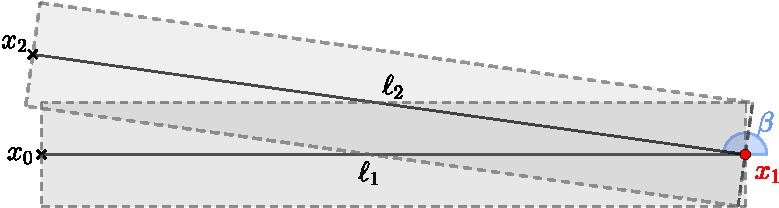
\includegraphics[width=.42\textwidth]{2D-1stOrderApproximation_rectangles_largeTA_largel2_nolabels-crop}}\hfill
	\subfloat[{Case 2: Large turning-angle with small $\ell_2$}]{%
		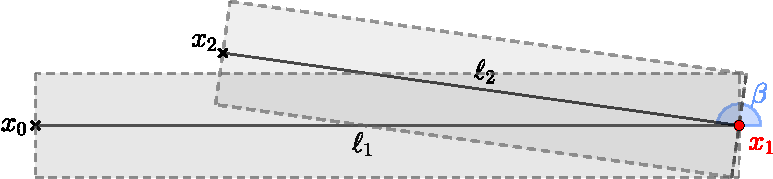
\includegraphics[width=.42\textwidth]{2D-1stOrderApproximation_rectangles_largeTA_smalll2_nolabels-crop}}\\
	\subfloat[Case 3: Medium turning-angle]{%
		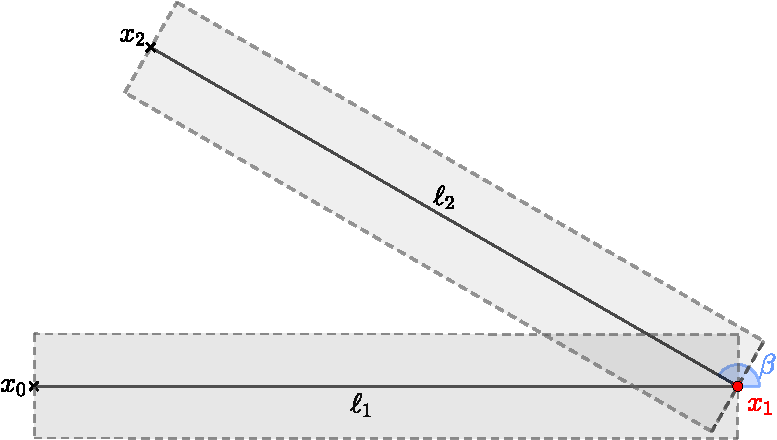
\includegraphics[width=.42\textwidth]{2D-1stOrderApproximation_rectangles_mediumTA_nolabels-crop}}\hfill
	\subfloat[Case 4: Small turning-angle]{%
		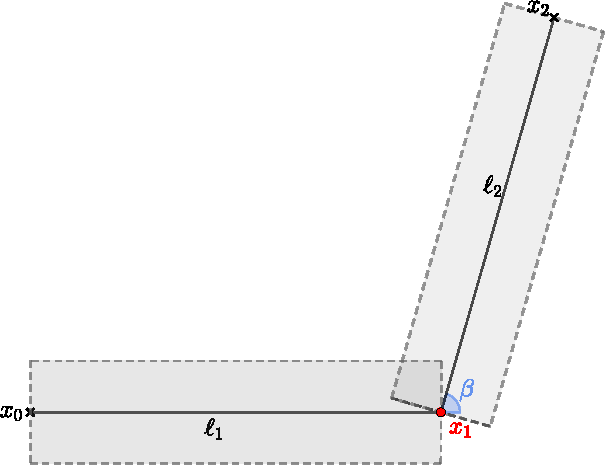
\includegraphics[width=.42\textwidth]{2D-1stOrderApproximation_rectangles_smallTA_nolabels-crop}}
	\caption[The four different cases for the turning-angle that we consider when determining the area of overlap]{The four cases that need to be considered to determine the overlapping area between two steps, with different turning-angles giving rise to different cases. When the turning-angle is large, which of case $1$ or case $2$ arise depends on the relative sizes of $\ell_1$ and $\ell_2$. When $\ell_2$ is sufficiently small, case $3$ becomes case $2$. Four more cases exist for turning-angles greater than $\pi$, although these are mirrors of the four cases above.}\label{fig:2d_model:firstorder:fourcasesappendix}
\end{figure}

\FloatBarrier
\paragraph{Case 1: Large turning-angle, large $\ell_2$}
\FloatBarrier
\begin{figure}[h!]
	\centering
	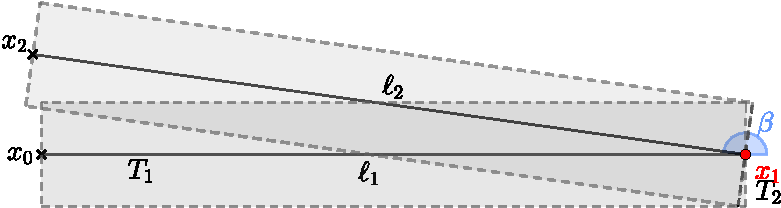
\includegraphics[width=1.0\textwidth]{2D-1stOrderApproximation_rectangles_largeTA_largel2-crop}
	\caption[Case 1: A large turning angle and large step]{Case 1: A large turning-angle and a large $\ell_2$. The bottom left triangle, $T_1$, and the bottom-right triangle, $T_2$, are labelled.}
	\label{fig:2d_model:firstorder:case1}
\end{figure}

For large turning-angles and large $\ell_2$, a large amount of overlap occurs. We consider a turning-angle to be large when the bottom parallel line to $\ell_2$ crosses the top parallel line of $\ell_1$. For this case, we require $\ell_2$ to be large enough relative to $\ell_1$ so that the $\ell_2$ rectangle extends out of the end of the $\ell_1$ rectangle, as it does in \cref{fig:2d_model:firstorder:case1}. The threshold length at which this occurs is when the horizontal component of $\ell_2$ is larger than $\ell_1$, which implies that we require $\ell_1 < -\ell_2 \cos (\beta)$. 

Note that there is not a clear transition between case $1$ and case $2$ at $\ell_1 = -\ell_2 \cos(\beta)$, but rather, there is a separate case entirely, since when $\ell_1$ is slightly smaller than $-\ell_2 \cos(\beta)$, geometry will arise that does not fall into either of the two cases. In this transition, both of the left-most corners will be outside of the $\ell_1$ rectangle while the line between the corners is within the rectangle, meaning a small triangle shaped area will be counted when it shouldn't. This can be seen in \cref{fig:2d_model:firstorder:case1-case2-threshold}. However, since this occurs only in a very specific situation, and the effect is very small, we disregard this and simply assume that case $2$ becomes case $1$ once $\ell_1 < -\ell_2 \cos(\beta)$.

\begin{figure}[h!]
	\centering
	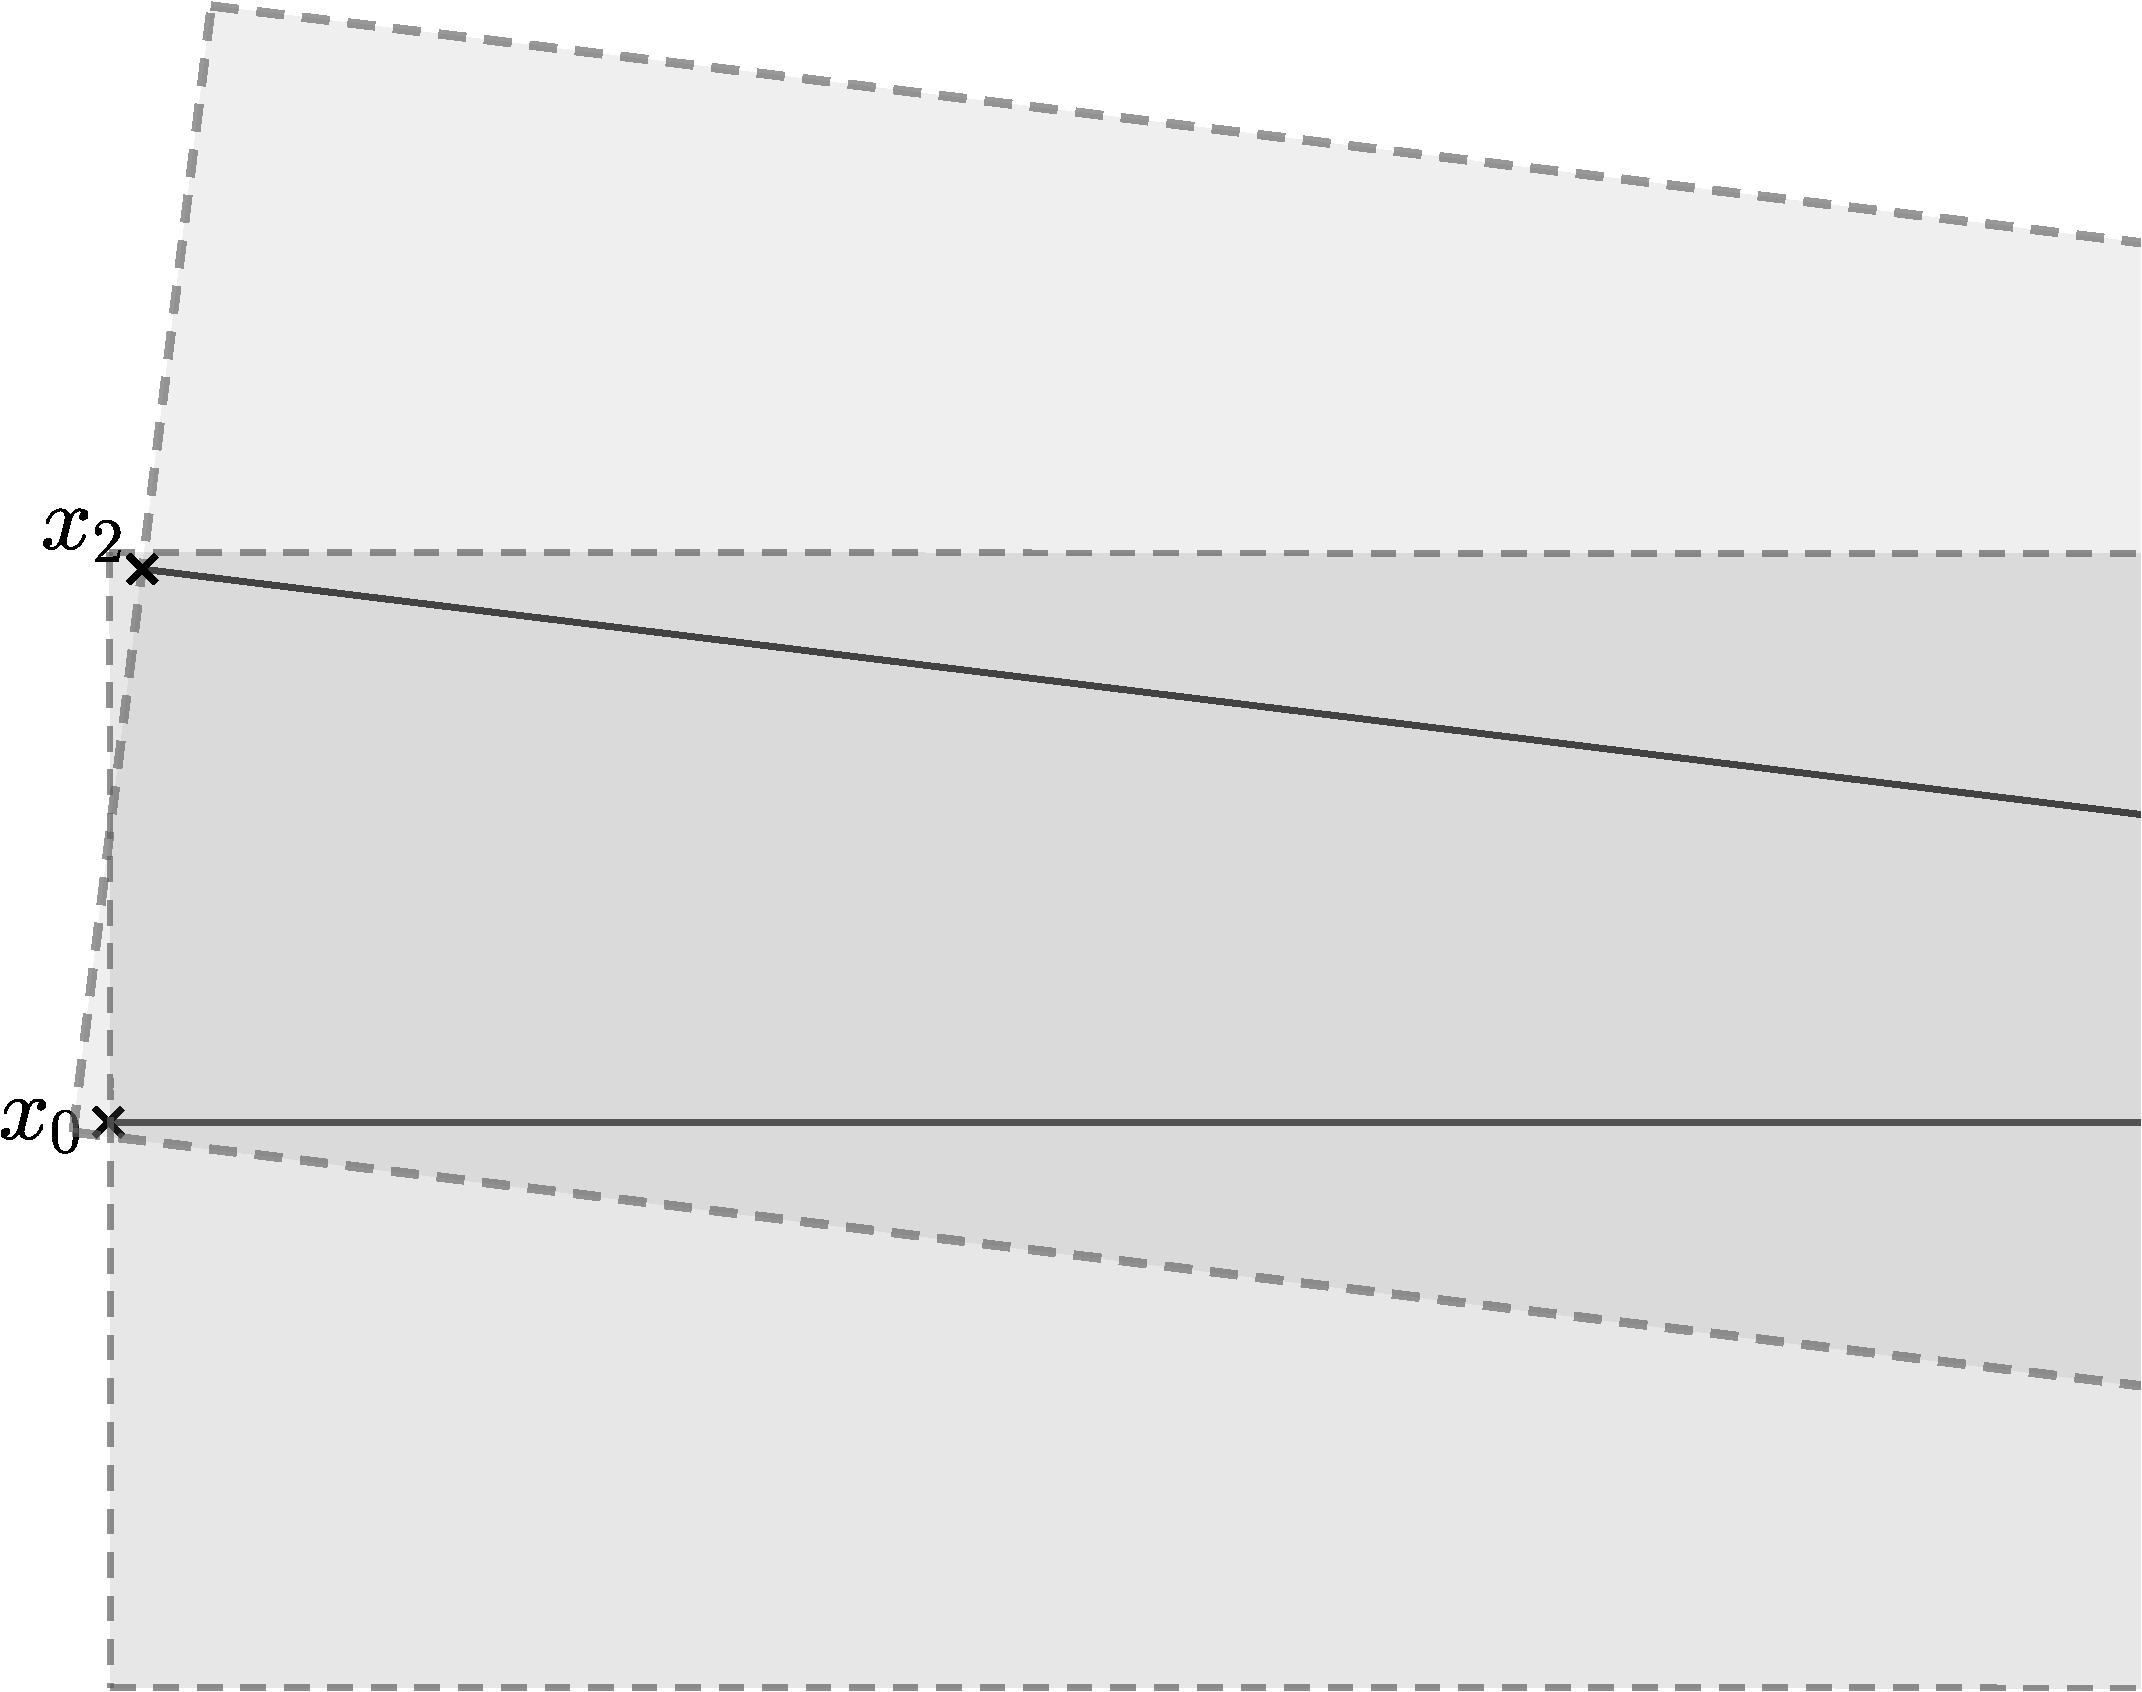
\includegraphics[width=1.0\textwidth]{2D-1stOrderApproximation_rectangles_largeTA_mediuml2-crop}
	\caption[There is no clear threshold between case $1$ and case $2$, although we assume that there is since the introduced error is only small]{There is not a clear threshold between case $1$ and case $2$, as can be seen in the above figure, which does not fall into either case. We assume that there is a clear threshold between the two cases, at the point when the bottom left corner of the $\ell_2$ rectangle exits the $\ell_1$ rectangle. The error caused by doing this will be small since the only difference is the small triangle on the left being counted as overlap when it should not be.}
	\label{fig:2d_model:firstorder:case1-case2-threshold}
\end{figure}

For case $1$, rather than find the area of overlap, it is easier to find the area of the $\ell_1$ rectangle that does not have any overlap.  This is the large right-angled triangle at the bottom, as well as the small right-angled triangle at the bottom right, which we denote $T_1$ and $T_2$ respectively. Note that the non-overlapping area isn't entirely made up of these two triangles since they do not perfectly meet the bottom of the $\ell_1$ rectangle, as seen in \cref{fig:2d_model:firstorder:case1-triangles}, although we assume that they do to avoid extra complications at the cost of a very small amount of accuracy. 

\begin{figure}[h!]
	\centering
	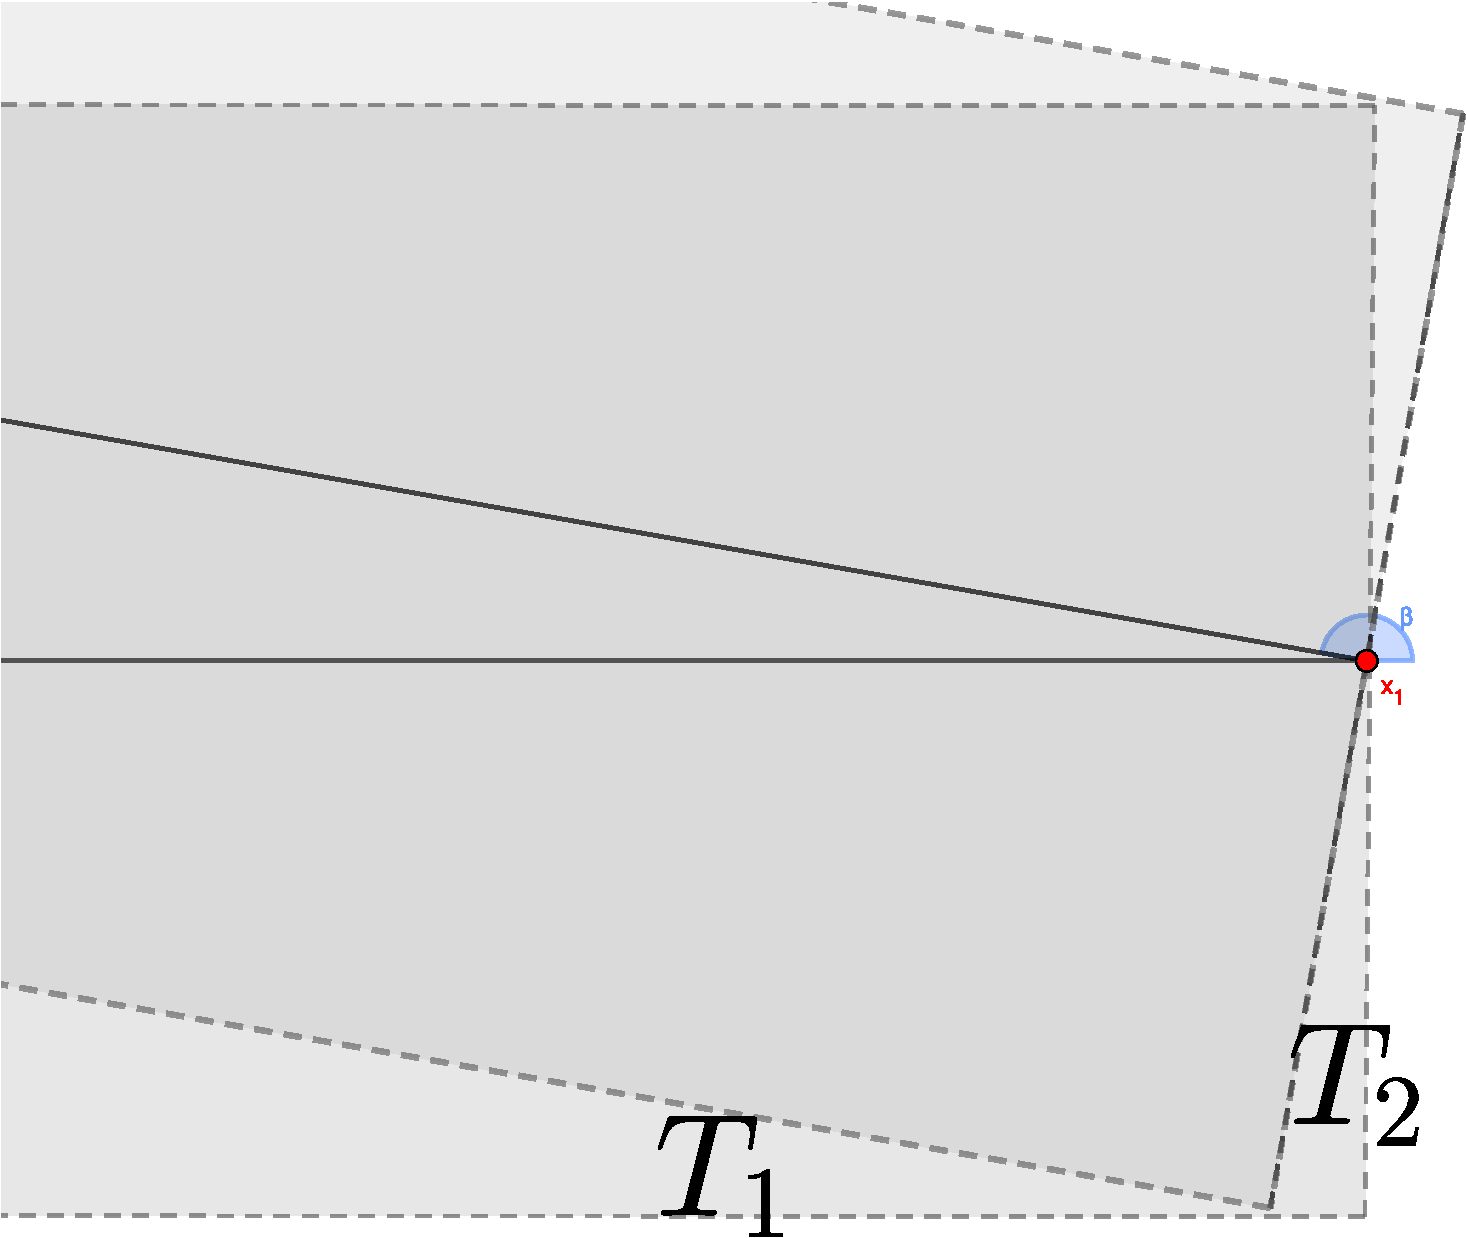
\includegraphics[width=1.0\textwidth]{2D-1stOrderApproximation_rectangles_largeTA_largel2_triangles-crop}
	\caption[A simplification that must be made in order to find the area for case 1]{The total unshaded area is not exactly $T_1 + T_2$, since the triangle $T_1$ does not meet the bottom line. The difference is so small that we assume they do meet, since it simplifies the calculations at the expense of very little error.}
	\label{fig:2d_model:firstorder:case1-triangles}
\end{figure}



The height of the triangle $T_2$ is $r_v$ and the angle at $x$ is $\pi-\beta$, and so the base must be $r_v\tan(\pi-\beta)$. Thus we get
\[A_{T_2} = \frac{-r_v^2}{2} \tan(\beta). \]
The base of triangle $T_1$ has length $\ell_1-r_v\tan(\pi-\beta) = \ell_1+r_v\tan(\beta)$, and the angle at the bottom-right of $T_1$ is $\pi - \beta$. The height of $T_1$ must therefore be
\[\tan(\pi-\beta) = h/(\ell_1+r_v\tan(\beta)) \implies h = -\ell_1 \tan(\beta)-r_v\tan^2(\beta). \]
The area of triangle $T_1$ is
\[A_{T_1} =(\ell_1+r_v\tan(\beta))(-\ell_1 \tan(\beta)-r_v\tan^2(\beta))/2 = \frac{-\left(\ell_1^2 \tan(\beta) + 2r_v\ell_1 \tan^2(\beta)+ r_v^2\tan^3(\beta)\right)}{2}, \]
and so the total area of overlap is
\begin{align*}
A_{\text{overlap}} &= 2 r_v \ell_1 - A_{T_1} - A_{T_2}\\
&=\frac{\ell_1^2 \tan(\beta) + 2r_v \ell_1(2+\tan^2(\beta))  + r_v^2 \tan^3(\beta)}{2}.
\end{align*}

\iffalse
Now, we determine the threshold angle at which the large turning-angle of case $1$ becomes a medium turning-angle of case $3$. We first determine the length along $\ell_2$ at which the line crosses the top edge of the $\ell_1$ rectangle. The top right of the $\ell_1$ rectangle is a right angle triangle with height $r_v$ and bottom right angle $\beta-\pi/2$. The hypotenuse must therefore be of length $r_v/\sin(\beta)$. The distance between the intersection of $\ell_2$ with the top of the $\ell_1$ rectangle, and the point $x_2$ must therefore be $\ell_2-r_v/\sin(\beta)$. We can construct a right angle triangle by drawing a line vertically down from $x_2$, which must have height $\ell_2\sin\beta-r_v$. The bottom left corner of the $\ell_2$ rectangle is a vertical distance of $-r_v\cos\beta$ below $x_2$. Thus, the height of the bottom left corner above $x_1$ is $\ell_2\sin\beta-r_v+r_v\cos\beta$. Then, the threshold angle is when this corner is above $x_1$ by $r_v$, and so we rearrange to get 
\fi

We can also use the height of triangle $T_1$ to determine the threshold angle at which the case of a large turning-angle becomes a medium turning-angle, and vice versa. When the height is greater than the width of the rectangle, $2r_v$, the turning-angle is considered medium. Thus, the threshold angle is
\[-\ell_1 \tan(\beta)-r_v = 2r_v \implies \beta^* = \pi+\arctan\left(\frac{-3r_v}{\ell_1}\right). \]

Therefore, case $1$ corresponds to $\pi+\arctan\left(\frac{-3r_v}{\ell_1}\right) \leq \beta \leq \pi$, and $\ell_1 < -  \ell_2 \cos (\beta)$.

For turning-angles larger than $\pi$, the same geometry will occur, but will be mirrored. The area for this will be
\[  A_{\text{overlap}} = \frac{-\ell_1^2 \tan(\beta) + 2r_v \ell_1(2+\tan^2(\beta))  - r_v^2 \tan^3(\beta)}{2},\]
since we must flip the sign of $\tan(\beta)$ in this range. This occurs for $\pi \leq \beta \leq \pi-\arctan\left(\frac{-3r_v}{\ell_1}\right)$, and $\ell_1 <-  \ell_2 \cos (\beta)$.

We can combine case $1$ and its mirror, by taking absolute values of $\tan(\beta)$, giving
\[  A_{\text{overlap}} = \frac{-\ell_1^2 \left|\tan(\beta)\right| + 2r_v \ell_1(2+\tan^2(\beta))  - r_v^2 \left|\tan^3(\beta)\right|}{2},\]
for $\pi+\arctan\left(\frac{-3r_v}{\ell_1}\right) \leq \beta \leq \pi-\arctan\left(\frac{-3r_v}{\ell_1}\right)$, and $\ell_1 < -  \ell_2 \cos (\beta)$.
\FloatBarrier
\paragraph{Case 2: Large turning-angle, small $\ell_2$}
\FloatBarrier
\begin{figure}[h!]
	\centering
	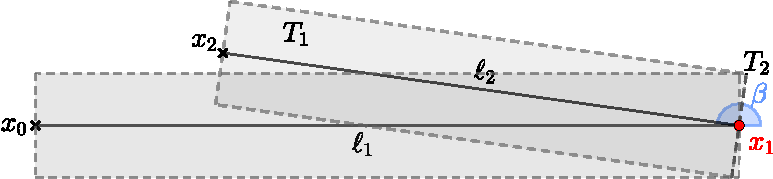
\includegraphics[width=1.0\textwidth]{2D-1stOrderApproximation_rectangles_largeTA_smalll2-crop}
	\caption[Case 2: A large turning-angle and a small step]{Case 2: A large turning-angle and a relatively small $\ell_2$. The top triangle, $T_1$, and the top-right triangle, $T_2$, are labelled.}
	\label{fig:2d_model:firstorder:case2}
\end{figure}
As discussed above, case $2$ occurs when $\ell_1 \geq -  \ell_2 \cos (\beta)$. We find the area of case $2$ in a very similar way to case $1$. This time we find the area of the $\ell_2$ rectangle that does not have overlap, and this is then the newly searched area. This non-overlapping area is once again made up of two triangles, which we denote $T_1$ and $T_2$. The area of the smaller triangle, $T_2$ is
\[A_{T_2} = \frac{-r_v^2}{2} \tan(\beta). \]
The base (top edge), of the larger triangle, $T_1$, is $\ell_2 +r_v\tan(\beta)$, and so the height is
\[\tan(\pi-\beta) = h/(\ell_2+r_v\tan(\beta)) \implies h = -\ell_2 \tan(\beta)-r_v \tan^2(\beta). \]
Therefore, the area of $T_1$ is
\begin{align*}
A_{T_1} &=(\ell_2+r_v\tan(\beta))(-\ell_2 \tan(\beta)-r_v\tan^2(\beta))/2\\ 
&= \frac{-\left(\ell_2^2 \tan(\beta) + 2r_v\ell_2 \tan^2(\beta)+ r_v^2\tan^3(\beta)\right)}{2}.
\end{align*}
The total area of overlap is therefore
\begin{align*}
A_{\text{overlap}} &= 2 r_v \ell_2 - A_{T_1} - A_{T_2}\\
&=\frac{\ell_2^2 \tan(\beta) + 2r_v \ell_2(2+\tan^2(\beta))  + r_v^2 \tan^3(\beta)}{2}.
\end{align*}

In this case, the threshold angle at which this case changes to case $3$ will also be different. As can be seen in \cref{fig:2d_model:firstorder:case2}, when the height of the unshaded triangle is greater than $2r_v$, case $2$ becomes case $3$. Since this unshaded section has hypotenuse $\ell_2$ and bottom-right angle $\pi-\beta$, we get that the height is $\ell_2 \sin(\beta)$, and so the threshold angle will be
\[\beta^* = \pi-\arcsin\left(\frac{2r_v}{\ell_2}\right).\]
and so case $2$ occurs when $\pi-\arcsin\left(\frac{2r_v}{\ell_2}\right) \leq \beta \leq \pi$ and $\ell_1 \geq -  \ell_2 \cos (\beta)$.

For angles greater than $\pi$, we get a mirror of case $2$, which occurs when $\pi \leq \beta \leq \pi +\arcsin\left(\frac{2r_v}{\ell_2}\right) $ and $\ell_1 \geq -  \ell_2 \cos (\beta)$. The area for this case will be
\[A_{\text{overlap}} =\frac{-\ell_2^2 \tan(\beta) + 2r_v \ell_2(2+\tan^2(\beta))  - r_v^2 \tan^3(\beta)}{2},\]
where we have changed the sign of $\tan$ from the original expression, as we did for case $1$.

We can combine case $2$ and its mirror, by taking absolute values of $\tan(\beta)$, giving
\[  A_{\text{overlap}} = \frac{-\ell_2^2 \left|\tan(\beta)\right| + 2r_v \ell_2(2+\tan^2(\beta))  - r_v^2 \left|\tan^3(\beta)\right|}{2},\]
for $\pi-\arcsin\left(\frac{2r_v}{\ell_2}\right) \leq \beta \leq \pi+\arcsin\left(\frac{2r_v}{\ell_2}\right)$, and $\ell_2 \geq -  \ell_1 \cos (\beta)$.
\FloatBarrier
\paragraph{Case 3: Medium turning-angle}
\FloatBarrier
\begin{figure}[h!]
	\centering
	\includegraphics[width=1.0\textwidth]{2D-1stOrderApproximation_rectangles_mediumTA-crop}
	\caption[Case 3: A medium turning-angle]{Case 3: A medium turning-angle. The overlapping area is made up of a right-angled triangle at the top, $T_1$, a kite, $K$, and a right-angled triangle at the bottom, $T_2$.}
	\label{fig:2d_model:firstorder:case3}
\end{figure}

For medium-sized turning-angles, substantially less overlap may occur, depending on the size of the angle. Looking at \cref{fig:2d_model:firstorder:case3}, we see that the overlapping region is made up of three separate shapes, a right-angle triangle in the top right, a parallelogram, and a right-angle triangle at the bottom, and we denote these as $T_1$, $P$, and $T_2$, respectively. Both triangles have the same area, as we will now show. The angle of $T_1$ at $x_1$ is clearly $\beta - \pi/2$, and so is the angle of $T_2$ at $x_1$. The length of the adjacent side to this angle for both triangles must be $r_v$. Then, the length of the opposite side will be 
\[r_v \tan (\beta - \pi/2) = -r_v \cot(\beta). \]
Thus, we get
\[A_{T_1} = A_{T_2} = \frac{-r_v^2}{2} \cot(\beta). \]
For the parallelogram, the bottom and the right edge are the hypotenuse for the bottom and top triangles, respectively. Thus, the edges each have length
\[\sqrt{ r_v^2 + r_v^2 \cot^2(\beta)    } = r_v \sqrt{1+ \cot^2(\beta)} = r_v \csc(\beta). \]
The angle between these edges is $\pi - \beta$, and so the total area of the parallelogram is
\[A_k = r_v^2 \csc^2(\beta) \sin(\pi - \beta)  = r_v^2 \csc(\beta).\]
Combining the three shapes give a total overlapping area of
\[A_{\text{overlap}} = A_{T_1} + A_k + A_{T_2} = r_v^2 \csc(\beta)-r_v^2 \cot(\beta) = r_v^2 \left( \csc(\beta) - \cot(\beta)\right). \]
We can further rearrange this to get
\[A_{\text{overlap}} =  \frac{r_v^2 \sin(\beta)}{1+\cos(\beta)}. \]
However, we need to keep in mind that the sign of the trigonometric functions may change throughout the range of $\beta$ for case $3$. To ensure this doesn't happen, we rewrite our expression as
\[A_{\text{overlap}} =  \frac{r_v^2 \left|\sin(\beta)\right|}{1-\left|\cos(\beta) \right|}. \]
This expression for the area is valid for the range $\pi/2 \leq \beta \leq \pi +\arctan\left(\frac{-3r_v}{\ell_2}\right)$.

This expression is also valid for the mirrored case when $\pi -\arctan\left(\frac{-3r_v}{\ell_2}\right) \leq \beta \leq 3\pi/2$.
\FloatBarrier
\paragraph{Case 4: Small turning-angle}
\begin{figure}[h!]
	\centering
	\includegraphics[width=0.8\textwidth]{2D-1stOrderApproximation_rectangles_smallTA-crop}
	\caption[Case 4: A small turning-angle]{Case 4: A small turning-angle. The overlapping area is made up of a quadrilateral, which we treat as two back-to-back right-angled triangles, $T_1$ and $T_2$.}
	\label{fig:2d_model:firstorder:case4}
\end{figure}
\FloatBarrier

When the turning angle is small, $0 \leq \beta \leq \pi/2$, only a very small amount of overlap will occur, as can be seen in \cref{fig:2d_model:firstorder:case4}. Since we require that $\lmin \geq r_v$, the length of $\ell_1$ and $\ell_2$ will not effect the overlap area for this case. The overlapping area is comprised of a kite, which in this case can be thought of as two right-angled triangles back-to-back. It is easy to see that the top-left angle of the quadrilateral will be $\pi -\beta$, and so the top-left angle for each of the two triangles will be $\pi/2 - \beta/2$. The length of the side opposite to this angle, for both triangles, is $r_v$. Therefore, the length of the adjacent side for both triangles will be
\begin{equation*}
\frac{r_v}{\tan(\pi/2-\beta/2)} = \frac{r_v}{\cot(\beta/2)} = r_v \tan(\beta/2).
\end{equation*}
Then, the total overlapping area will be the sum of the area of both triangles,
\begin{equation*}
A_{\text{overlap}} = r_v^2 \tan(\beta/2).
\end{equation*}
When making a small turn in the opposite direction, $-\pi/2 \leq \beta \leq 0$, we switch the sign of $\tan(\beta)$ to get
\begin{equation*}
A_{\text{overlap}} = -r_v^2 \tan(\beta/2).
\end{equation*}

\paragraph{Combining the four cases}
Combining each of the four cases, when $\ell_1 \geq -\ell_2 \cos(\beta)$,  the total area of overlap is
\begin{equation*}
A_{\text{overlap}} = 
\begin{cases}
r_v^2 \left|\tan(\beta/2)\right| \quad &\text{if } \beta \leq \pi/2, \text{ or } \beta \geq 3\pi/2,\\\\
\displaystyle \frac{r_v^2 \left|\sin(\beta)\right|}{1-\left|\cos(\beta) \right|} &\text{if } \pi/2  \leq \beta \leq  \pi-\arcsin\left( \frac{2r_v}{\ell_2} \right),\\
&\text{or }\pi+\arcsin\left( \frac{2r_v}{\ell_2} \right) \leq \beta \leq 3\pi/2,\\\\
\displaystyle \frac{1}{2} \left[-\ell_2^2 \left|\tan(\beta)\right| + 2r_v \ell_2(2+\tan^2(\beta))\right.  &\text{if }\pi-\arcsin\left( \frac{2r_v}{\ell_2} \right) \leq \beta,\\
\left.  - r_v^2 \left|\tan^3(\beta)\right| \right]   &\text{and } \beta \leq \pi +\arcsin\left( \frac{2r_v}{\ell_2} \right),
\end{cases}
\end{equation*}
and when $\ell_1  < -\ell_2 \cos(\beta)$, the overlap is
\begin{equation*}
A_{\text{overlap}} = 
\begin{cases}
r_v^2 \left|\tan(\beta/2)\right| \quad &\text{if } \beta \leq \pi/2, \text{ or } \beta \geq 3\pi/2,\\\\
\displaystyle \frac{r_v^2 \left|\sin(\beta)\right|}{1-\left|\cos(\beta) \right|} &\text{if } \pi/2  \leq \beta \leq  \pi+\arctan\left( \frac{-3r_v}{\ell_1} \right),\\
&\text{or }\pi-\arctan\left( \frac{-3r_v}{\ell_1} \right) \leq \beta \leq 3\pi/2,\\\\
\displaystyle \frac{1}{2} \left[-\ell_1^2 \left|\tan(\beta)\right| + 2r_v \ell_1(2+\tan^2(\beta))\right.   &\text{if }\pi+\arctan\left( \frac{-3r_v}{\ell_1} \right) \leq \beta,\\
\left.- r_v^2 \left|\tan^3(\beta)\right| \right]   &\text{and } \beta \leq \pi -\arctan\left( \frac{-3r_v}{\ell_1} \right).
\end{cases}
\end{equation*}

The angles at which the expressions change depend on the length of the steps, and the lengths at which the expressions change depend on the angle. To get around this, we simplify our expressions by replacing the condition $\ell_1 < -\ell_2 \cos(\beta)$ with $\ell_1 < \ell_2$, introducing another small amount of error. Now, note that when $\ell_1 \approx \ell_2$ and $\ell_2 \gg r_v$, then $\arctan\left( \frac{-3r_v}{\ell_1}\right) \approx -\arcsin\left( \frac{2r_v}{\min(\ell_1,\ell_2)} \right)$. Thus, the function for the overlapping area becomes
\begin{equation*}
A_{\text{overlap}} = 
\begin{cases}
r_v^2 \left|\tan(\beta/2)\right| \quad &\text{if } \beta \leq \pi/2 \text{ or } \beta \geq 3\pi/2,\\\\
\displaystyle \frac{r_v^2 \left|\sin(\beta)\right|}{1-\left|\cos(\beta) \right|} &\text{if } \pi/2  \leq \beta \leq  \pi-\arcsin\left( \frac{2r_v}{\min(\ell_1,\ell_2)} \right),\\
&\text{or }\pi+\arcsin\left( \frac{2r_v}{\min(\ell_1,\ell_2)} \right) \leq \beta \leq 3\pi/2\\\\
\displaystyle \frac{1}{2} \left[-\min(\ell_1,\ell_2)^2 \left|\tan(\beta)\right| \right. &\text{if }\pi-\arcsin\left( \frac{2r_v}{\min(\ell_1,\ell_2)} \right) \leq \beta\\
\left.+ 2r_v \min(\ell_1,\ell_2)(2+\tan^2(\beta))\right.  &\text{and } \beta \leq \pi +\arcsin\left( \frac{2r_v}{\min(\ell_1,\ell_2)} \right).\\
\left. - r_v^2 \left|\tan^3(\beta)\right| \right]   
\end{cases}
\end{equation*}

Then, the total area covered by a step of length $\ell_2$, and with turning-angle $\beta$, with previous step-length $\ell_1$ will be
\begin{equation*}
A = 2\ell_2 r_v - A_{\text{overlap}}.
\end{equation*}
\backmatter
% Add the bibliography to the table of contents
\addcontentsline{toc}{chapter}{Bibliography}

\printbibliography

\end{document}
